% !TEX TS-program = pdflatex
% !TEX encoding = UTF-8 Unicode

% This is a simple template for a LaTeX document using the "article" class.
% See "book", "report", "letter" for other types of document.

\documentclass[11pt]{article} % use larger type; default would be 10pt


\usepackage[utf8]{inputenc} % set input encoding (not needed with XeLaTeX)

%%% Examples of Article customizations
% These packages are optional, depending whether you want the features they provide.
% See the LaTeX Companion or other references for full information.

%%% PAGE DIMENSIONS
\usepackage{geometry} % to change the page dimensions
\geometry{a4paper} % or letterpaper (US) or a5paper or....
% \geometry{margin=2in} % for example, change the margins to 2 inches all round
% \geometry{landscape} % set up the page for landscape
%   read geometry.pdf for detailed page layout information

\usepackage{graphicx} % support the \includegraphics command and options

% \usepackage[parfill]{parskip} % Activate to begin paragraphs with an empty line rather than an indent

%%% PACKAGES
\usepackage{booktabs} % for much better looking tables
\usepackage{array} % for better arrays (eg matrices) in maths
\usepackage{paralist} % very flexible & customisable lists (eg. enumerate/itemize, etc.)
\usepackage{verbatim} % adds environment for commenting out blocks of text & for better verbatim
 % make it possible to include more than one captioned figure/table in a single float
% These packages are all incorporated in the memoir class to one degree or another...

\usepackage[export]{adjustbox}
\usepackage{graphicx}
\usepackage{amssymb}
\usepackage{hyperref}
\hypersetup{
    colorlinks=true,
    linkcolor=blue,
    filecolor=magenta,      
    urlcolor=cyan,
}
\usepackage{relsize}
\usepackage[utf8]{inputenc}
\usepackage[LGR]{fontenc}
\usepackage[T1]{fontenc}
\usepackage[greek,english]{babel}
\usepackage{alphabeta}
\usepackage{amsmath}
\usepackage{physics}
\usepackage{amsfonts}
\usepackage{nccmath}
\usepackage[overload]{empheq}
\usepackage{float}
\usepackage{caption}
\usepackage{subcaption}
\restylefloat{table}
\usepackage{afterpage}
\usepackage[nottoc,notlot,notlof]{tocbibind}


\newcommand\blankpage{%
    \null
    \thispagestyle{empty}%
    \addtocounter{page}{-1}%
    \newpage}




 






%%% HEADERS & FOOTERS
\usepackage{fancyhdr} % This should be set AFTER setting up the page geometry
\pagestyle{fancy} % options: empty , plain , fancy
\renewcommand{\headrulewidth}{0pt} % customise the layout...
\lhead{}\chead{}\rhead{}
\lfoot{}\cfoot{\thepage}\rfoot{}

%%% SECTION TITLE APPEARANCE
\usepackage{sectsty}
\allsectionsfont{\sffamily\mdseries\upshape} % (See the fntguide.pdf for font help)
% (This matches ConTeXt defaults)

%%% ToC (table of contents) APPEARANCE
\usepackage[nottoc,notlof,notlot]{tocbibind} % Put the bibliography in the ToC
\usepackage[titles,subfigure]{tocloft} % Alter the style of the Table of Contents
\renewcommand{\cftsecfont}{\rmfamily\mdseries\upshape}
\renewcommand{\cftsecpagefont}{\rmfamily\mdseries\upshape} % No bold!

%%% END Article customizations

%%% The "real" document content comes below...
\addto\captionsenglish{\renewcommand*\contentsname{Περιεχόμενα}}
\addto\captionsenglish{\renewcommand*\refname{Βιβλιογραφία}}
\addto\captionsenglish{\renewcommand{\figurename}{Εικόνα}}
\addto\captionsenglish{\renewcommand{\tablename}{Πίνακας}}


\title{
    {
\includegraphics[width=0.2\textwidth]{emp.jpg}}\\
    {\large  Εθνικό Μετσόβιο Πολυτεχνείο}\\
    {\large  Τμήμα Χημικών Μηχανικών}\\
    {Ανάπτυξη Μεθοδολογίας Αυτόματης Ρύθμισης Συστημάτων με Εκπαίδευση Νευρωνικών Δικτύων Βάθους}\\
}
\author{Στεφανής Μιχαήλ}




\numberwithin{equation}{subsection}

\begin{document}
\maketitle
\begin{figure}[H]
    \centering
    
\includegraphics[width=0.9\textwidth]{intro.jpeg}
\end{figure}
\newpage

\tableofcontents



\newpage






\section{Εισαγωγή}
Στην παρούσα διπλωματική εργασία εξετάζεται η δυνατότητα \textit{ανάπτυξης μεθοδολογίας αυτόματης ρύθμισης συστημάτων με την χρήση τεχνικών τεχνητής νοημοσύνης}. Πιο συγκεκριμένα, εξετάζεται η δυνατότητα σχεδιασμού ενός ρυθμιστή, η λειτουργία του οποίου θα βασίζεται τόσο στην \textit{Εκπαίδευση Νευρωνικών Δικτύων Βάθους} (Deep Learning) όσο και στην θεωρία της \textit{Ενισχυτικής Μάθησης} (Reinforcement Learning). Η προτεινόμενη μεθοδολογία, ονόματι \textit{Βαθμίδα Ντετερμινιστικής Πολιτικής Βάθους} (Deep Deterministic Policy Gradient, DDPG) \cite{deepmind}, αναπτύχθηκε από την DeepMind το 2016 με σκοπό την ρύθμιση συστημάτων που χαρακτηρίζονται από συνεχές πεδίο τιμών των μεταβλητών εισόδου και εξόδου. Η εν λόγω προσέγγιση ρύθμισης βασισμένη στον αλγόριθμο DDPG έχει ένα μεγάλο πλεονέκτημα σε σχέση με τα συμβατικά συστήματα ρύθμισης, όπως ο PID και η LQR. Τα συστήματα αυτά προκειμένου να λειτουργήσουν έχουν ανάγκη το ίδιο το μοντέλο της διεργασίας, δηλαδή έναν νόμο ελέγχου. Είναι δηλαδή Model-Based συστήματα ρύθμισης. Το προτεινόμενο σύστημα ρύθμισης όμως δεν έχει αναγκή να γνωρίζει το μοντέλο της διεργασίας επειδή βασίζεται στην \textit{εξερεύνηση} του χώρου μέσα στον οποίο ζει η διεργασία (ο οποίος φυσικά περιγράφεται από κάποιες εξισώσεις). Αυτή είναι η ριζική διαφορά που κάνει το εν λόγω σύστημα ρύθμισης τόσο ελκυστικό. Έχοντας μηδενική γνώση της διεργασίας και του μοντέλου της μπορούμε να προσεγγίσουμε μία επιθυμητή μόνιμη κατάσταση εξερευνώντας και \textit{μαθαίνοντας} το περιβάλλον.\\

Η πορεία μέχρι να είμαστε σε θέση να παρουσιάσουμε τον βασικό αλγόριθμο ρύθμισης, DDPG, είναι μεγάλη. Θα αρχίσουμε παρουσιάζοντας κάποια γενικά στοιχεία που αφορούν την μηχανική μάθηση σαν επιστήμη, εφόσον τα νευρωνικά δίκτυα και η ενισχυτική μάθηση υπάγονται σε αυτήν. Στην συνέχεια θα εξετάσουμε κάποια πολύ βασικά στοιχεία του κλάδου της ρύθμισης διεργασιών έτσι ώστε να μπορέσουμε να τοποθετηθούμε καλύτερα στο τελικό μας πρόβλημα ρύθμισης. Έπειτα θα γίνει μία πολύ αναλυτική περιγραφή της εκπαίδευσης ενός νευρωνικού δικτύου βάθους (Deep Learning) καθώς και μία εισαγωγή στην θεωρία της Ενισχυτικής Μάθησης (Reinforcement Learning) αλλά και στις βασικές εξισώσεις που την συνιστούν, τις εξισώσεις Bellman. Έχοντας τις δύο αυτές βασικές θεωρίες θα τις συνδυάσουμε με έναν αρκετά φιλοσοφημένο και έξυπνο τρόπο για να εξάγουμε την θεωρία της \textit{Ενισχυτικής Μάθησης Βάθους} (Deep Reinforcement Learning), πάνω στην οποία βασίζεται και ο αλγόριθμος DDPG. Τότε και μόνο τότε θα είμαστε έτοιμοι να παρουσιάσουμε και να περιγράψουμε τον αλγόριθμο αλλά και να συνεχίσουμε με εφαρμογές, αποτελέσματα και σχολιασμούς. Στο τέλος της εργασίας παρατίθεται και ένα παράρτημα το οποίο είναι κυρίως μαθηματικού περιεχόμενου και περιέχει αποδείξεις διαφόρων θεωρημάτων και εξισώσεων που παρουσιάζονται ή/και χρησιμοποιούνται κατα μήκος όλης της εργασίας. 

\newpage

\section{Μηχανική Μάθηση}

\subsection{Εισαγωγή}


Η \textit{Μάθηση}, όπως και η νοημοσύνη, καλύπτουν ένα πολύ ευρή φάσμα διαδικασιών που είναι δύσκολο να ορισθεί ακριβώς. Ορισμοί που συναντούμε συνήθως σε ένα λεξικό ή στο διαδίκτυο περιλαμβάνει φράσεις όπως "η απόκτηση γνώσεων και ικανοτήτων μέσα από μελέτη, οδηγίες ή εμπειρίες". Υπάρχουν αρκετοί παραλληλισμοί μεταξύ της βιολογικής και της μηχανικής μάθησης. Πράγματι, πολλές τεχνικές της μηχανικής μάθησης εξάγονται από τις προσπάθειες ψυχολόγων να βελτιώσουν τις θεωρίες τους πάνω στην βιολογική μάθηση μέσα από υπολογιστικά μοντέλα \cite{machinelearning1}. Ακόμα πιο εντυπωσιακό είναι το αντίστροφο. Πολλές έννοιες και τεχνικές που χρησιμοποιούνται από ερευνητές της μηχανικής μάθησης μπορούν να δώσουν φως σε μυστήρια που σχετίζονται με την βιολογική μάθηση. Στο κεφάλαιο αυτό θα ασχοληθούμε μόνο με την μηχανική μάθηση.\\


Η Μηχανική Μάθηση είναι ένας υποκλάδος της επιστήμης των υπολογιστών που εξελήχθηκε από την μελέτη της αναγνώρισης προτύπων και υπολογιστικής θεωρίας μάθησης στην τεχνητή νοημοσύνη. To 1959, ο Arthur Samuel όρισε την μηχανική μάθηση ως "Το αντικείμενο μελέτης που δίνει στους υπολογιστές την ικανότητα να μάθουν χώρις να προγραμματίζονται με ρητό και καθορισμένο τρόπο" \cite{machinelearning2}. Το αντικείμενο της μηχανικής μάθησης είναι η κατασκευή και η μελέτη δυναμικών αλγορίθμων που μπορούν να \textit{μάθουν} και να \textit{κάνουν προβλέψεις} με βάση κάποια δεδομένα. Αυτού του είδους οι αλγόριθμοι λειτουργούν κατασκευάζοντας ένα \textit{μοντέλο} από δεδομένα εισόδου με σκοπό να κάνουν προβλέψεις και να παίρνουν αποφάσεις καθοδηγούμενα από τα ίδια τα δεδομένα αντί να ακολουθούν αυστηρά κάποιο στατικό πρόγραμμα. Πρόκειται δηλαδή για την υλοποίηση ενός \textit{δυναμικού} κώδικα ο οποίος θα μπορεί να προσαρμόζεται σε νέα δεδομένα, όπως ακριβώς ένας άνθρωπος μαθαίνει να προσαρμόζεται σε νέες καταστάσεις με την βοήθεια της εμπειρίας του και των γνώσεων που έχει αποκτήσει στο παρελθόν. \\

Η μηχανική μάθηση είναι στενά συνδεδεμένη με την υπολογιστική στατιστική, μία μαθηματική θεωρία που εξειδικεύεται στις προβλέψεις και είναι με την σειρά της συνδεδεμένη με την μαθηματική έννοια της \textit{βελτιστοποίησης}. Το εύρος των εφαρμογών της μηχανικής μάθησης είναι εκπληκτικά μεγάλο όμως η μηχανική μάθηση αριστεύει στις εφαρμογές στις οποίες ο σχεδιασμός ενός (στατικού) προγράμματος-αλγορίθμου είναι αδύνατος. Παραδείγματα εφαρμογών είναι η \textit{οπτική αναγνώριση χαρακτήρων} (γραμμάτων και αριθμών), οι \textit{μηχανές αναζήτησης}, και το  \textit{φιλτράρισμα ανεπιθύμητων μηνυμάτων} (spam filtering) \cite{machinelearning2}.\\

\subsection{Τύποι προβλημάτων μηχανικής μάθησης}
Τα προβλήματα στην μηχανική μάθηση συνήθως κατηγοριοποιούνται σε τρεις μεγάλες κατηγορίες με βάση την φύση των δεδομένων που είναι διαθέσιμα στο σύστημα εκμάθησης. Οι τρεις αυτές κατηγορίες είναι οι εξής \cite{machinelearning2}:\\

\begin{itemize}
\item \textbf{Εποπτευόμενη Μάθηση} (Supervised Learning): Στον υπολογιστή παρουσιάζονται τα δεδομένα εισόδου αλλά και οι επιθυμητές έξοδοι, οι οποίες παρατίθενται από τον προγραμματιστή, και ο στόχος είναι να βρεθεί (να μαθευτεί) ένας κανόνας, μία δηλαδή \textit{συνάρτηση}, η οποία θα συσχετίζει την είσοδο με την έξοδο. Πρόκειται δηλαδή για προβλήματα στα οποία γνωρίζουμε από που αρχίζουμε αλλά και που θέλουμε να καταλήξουμε. Χαρακτηριστικό παράδειγμα είναι η αναγνώριση χαρακτήρων \cite{neuralnets3}, όπου δίνουμε στον υπολογιστή, για παράδειγμα, αφενός τυχαίους φυσικούς αριθμούς (από το 0 μέχρι το 9) που έχουν γραφτεί από ανθρώπινο χέρι και αφετέρου τους ίδιους αριθμούς που όμως έχουν γραφτεί από υπολογιστή (και είναι κατά μία έννοια "τέλειοι"). Στόχος της μηχανικής μάθησης είναι να καταφέρει εν τέλει ο υπολογιστής να δεχθεί έναν χαρακτήρα που είναι γραμμένος από άνθρωπο και να μπορέσει να μας δώσει τον αντίστοιχο σωστό χαρακτήρα στην οθόνη του. \\
\item \textbf{Μη-Εποπτευόμενη Μάθηση} (Unsupervised Learning): Στην περίπτωση αυτή τα δεδομένα εξόδου δεν δίνονται και αφήνουμε τον υπολογιστή να βρει ο ίδιος μία εσωτερική δομή-μοτίβο στα δεδομένα εισόδου. Τα προβλήματα αυτά είναι κατά κανόνα πιο απαιτητικά, απαιτούν μεγαλύτερο όγκο δεδομένων και συνήθως πρόκειται περί προβλημάτων ομαδοποίησης.\\
\item \textbf{Ενισχυτική Μάθηση} (Reinforcement Learning): Στην ενισχυτική μάθηση ένα πρόγραμμα του υπολογιστή αλληλεπιδρά με ένα δυναμικό περιβάλλον στο οποίο θα πρέπει να πετύχει έναν συγκεκριμένο στόχο (όπως, για παράδειγμα, να οδηγήσει ένα όχημα) χωρίς κάποιον εξωτερικό πληροφοριοδότη για να του πει κατά πόσο έχει φτάσει κοντά στον στόχο του. Ένα παράδειγμα εφαρμογής της ενισχυτικής μάθησης είναι η ικανότητα ενός υπολογιστή να μάθει να παίζει ένα παιχνίδι (για παράδειγμα σκάκι) καθώς παίζει με έναν αντίπαλο. Το εκπληκτικό χαρακτηριστικό της ενισχυτικής μάθησης είναι ότι ο υπολογιστής δεν απαιτείται να έχει καμία πληροφορία για το (στην συγκεκριμένη περίπτωση) παιχνίδι, δηλαδή για τους κανόνες του παιχνιδιού. Μαθαίνει ό,τι πληροφορία είναι απαραίτητη για να κερδίσει μέσα από την εμπειρία που κερδίζει από τα πολλά παιχνίδια \cite{reinflearning}.
\end{itemize}

Μία άλλη κατηγοριοποίηση προβλημάτων μηχανικής μάθησης προκύπτει ανάλογα με την \textit{επιθυμητή έξοδο} του συστήματος μάθησης \cite{machinelearning2}:\\

\begin{itemize}
\item \textbf{Ταξινόμηση (Classification)}: Στα προβλήματα ταξινόμησης τα δεδομένα χωρίζονται σε δύο ή περισσότερες κλάσσεις και το σύστημα εκμάθησης πρέπει να παράξει ένα μοντέλο το οποίο να εισάγει μία άγνωστη είσοδο σε μία από αυτές τις κλάσσεις. Συνήθως πρόκειται για εποπτευόμενα προβλήματα. Το φιλτράρισμα ανεπιθύμητων μηνυμάτων ανήκει στα προβλήματα ταξινόμησης. Τα εισερχόμενα μηνύματα είναι η είσοδος και οι κλάσσεις είναι "Ανεπιθύμητο" και "Επιθυμητό". Ένα άλλο παράδειγμα είναι η ταξινόμηση ανθρώπων με βάση το φύλο. Σε μία κάμερα μπορεί να εισαχθεί ένα πρόγραμμα το οποίο θα αποφασίζει αν ένας άνθρωπος είναι "άντρας" ή "γυναίκα" (οι δύο κλάσσεις) με βάση χαρακτηριστικά όπως τα μαλλιά, το μέγεθος των χεριών κ.α.  \\
\item \textbf{Παλινδρόμηση (Regression)}: Τα προβλήματα παλινδρόμησης είναι και αυτά εποπτευόμενα προβλήματα όμως, σε αντίθεση με τα προβλήματα ταξινόμησης, οι έξοδοι του συστήματος είναι συνεχής ποσότητες αντι για διακριτές. Ένα πολύ γνωστό παράδειγμα παλινδρόμησης είναι η λεγόμενη \textit{γραμμική παλινδρόμηση} κατά την οποία, στις δύο διαστάσεις, προσπαθούμε να προσδιορίσουμε μία ευθεία γραμμή η οποία να ταιριάζει όσο το δυνατόν καλύτερα στα δεδομένα μάς. \\
 \item \textbf{Ομαδοποίηση (Clustering)}: Στα προβλήματα ομαδοποίησης ένα σύνολο δεδομένων εισόδου χωρίζεται σε ομάδες. Σε αντίθεση με την περίπτωση της ταξινόμησης, οι ομάδες-κλάσσεις δεν είναι γνωστές εκ των προτέρων, κάτι που καθιστά τα προβλήματα αυτά μη-εποπτευόμενα.\\
\item \textbf{Εκτίμηση Πυκνότητας (Density Estimation)}: Το πρόβλημα σε αυτήν την περίπτωση είναι η εύρεση της κατανομής των δεδομένων εισόδου που ορίζονται σε κάποιον χώρο.\\ 
\item \textbf{Μείωση Διαστατικότητας (Dimensionality Reduction)}: Στα προβλήματα αυτά τα δεδομένα εισόδου απλοποιούνται απεικονίζοντάς τα σε κάποιον χώρο μικρότερης διάστασης. Παράδειγμα τέτοιου προβλήματος είναι το λεγόμενο \textit{Topic Modeling}. Σε ένα πρόγραμμα υπολογιστή δίνουμε μία λίστα από έγγραφα γραμμένα σε κάποια γλώσσα και το ζητούμενο του υπολογιστή είναι να βρει ποια έγγραφα πραγματεύονται παρόμοια θέματα.
\end{itemize}


\newpage

\section{Ρύθμιση Διεργασιών}


\subsection{Εισαγωγή}
Εφόσον εξετάζεται η δυνατότητα εύρεσης παραμέτρων ενός ρυθμιστή βασισμένου σε μεθοδολογίες τεχνιτής νοημοσύνης, θα πρέπει να εξετάσουμε τα βασικά δομικά στοιχεία του κλάδου της ρύθμισης διεργασιών.\\

Γενικά με τον όρο "\textit{ρύθμιση}" εννοούμε, εν γένει, την ανάλήψη και την οργάνωση δράσεως προς διατήρηση των επιθυμητών συνθηκών σε μία οποιαδήποτε διεργασία. Η διεργασία αυτή είναι δυνατόν να είναι μηχανική, χημική, ηλεκτρική ή/και συνδυασμός αυτών \cite{daoutidhs}. Αυτή η δράση είναι δυνατόν να πραγματοποθηθεί είτε μέσω ανθρώπινης παρέμβασης (χειρισμό) ή και με κάποιο μηχανισμό. Στις εφαρμογές, η ρύθμιση αποβλέπει στην επίτευξη των επιθυμητών συνθηκών λειτουργίας και, κυρίως, στην δυνατότητα επαναφοράς στις επιθυμητές αυτές συνθήκες, όταν υπάρξει κάποια διαταραχή, όπως και στην δυνατότητα επιτεύξεως μόνιμης καταστάσεως όταν ένα ή/και περισσότερα εξωτερικά αίτια τείνουν να δημιουργήσουν μεταβατικές συνθήκες. Προκειμένου να υπάρχει ρύθμιση μίας διεργασίας, χρησιμοποιούμε σε κάθε περίπτωση μετρητικά, ρυθμιστές και τελικά στοιχεία ρύθμισης. Οι βασικοί στόχοι της ρύθμισης αφορούν πλέον την συμπεριφορά του συνολικού συστήματος και είναι οι εξής \cite{daoutidhs}:\\

\begin{itemize}
  \item \textbf{Ευστάθεια}: Στις περισσότερες εφαρμογές της ρύθμισης θέλουμε το σύστημά μας να "ισορροπίσει" σε μία μόνιμη κατάσταση η οποία να είναι \textit{ευσταθής}. Στην ουσία αυτό σημαίνει ότι αν στο σύστημα που ισορροπεί ασκηθεί μία (απρόβλεπτη) επιβολή τότε αυτό θα πρέπει να μπορέσει να επανέλθει στην προηγούμενη κατάσταση ισορροπίας. Φυσικά ο ρυθμιστής σε καμία περίπτωση δεν θα πρέπει να χαλάει την ευστάθεια του συστήματος. 
  \item \textbf{Απόσβεση των διαταραχών}: Όπως θα δούμε παρακάτω, οι διαταραχές είναι μεταβλητές του συστήματος τις οποίες ο άνθρωπος δεν μπορεί να ελέγξει και να ρυθμίσει. Το σύστημα της ρύθμισης θα πρέπει να μπορεί να ανταπεξέλθει στην ύπαρξη αυτών των διαταραχών και να ρυθμίσει το σύστημα στο οποίο εμφανίζονται. Αυτό σημαίνει ότι αν μία διαταραχή απομακρύνει το σύστημα από την κατάσταση ισορροπίας του τότε ο ρυθμιστής θα πρέπει να είναι σε θέση να το επαναφέρει.  
  \item \textbf{Ικανότητα καθοδηγητικού ελέγχου}: Στις περισσότερες πραγματικές εφαρμογές ρύθμισης είναι συχνά επιθυμητό, είτε για λόγους ασφάλειας είτε για λόγους παραγωγικότητας, η μόνιμη κατάσταση του συστήματος να αλλάξει. Στις περιπτώσεις αυτές θα πρέπει ο ρυθμιστής να μπορεί να "καθοδηγήσει" με ασφάλεια και όσο το δυνατόν πιο γρήγορα το σύστημα στην νέα αυτή μόνιμη κατάσταση. 
  \item \textbf{Ευρωστία}: Το σύστημα ρύθμισης οφείλει να μπορεί να αναπεξέλθει σε απρόβλεπτες καταστάσεις που σχετίζονται με εξωτερικά φαινόμενα, όπως οι καιρικές συνθήκες ή/και φαινόμενα όπως οι σεισμοί. Θα πρέπει, για παράδειγμα, να διαθέτει "εργαλεία" τα οποία να μπορούν να ρυθμίσουν επιτυχώς το σύστημα ακόμα και μία πολύ ζεστή καλοκαιρινή μέρα, όπου η θερμοκρασία του περιβάλλοντος μπορεί να είναι αρκετά μεγαλύτερη από την θερμοκρασία στην οποία σχεδιάστηκε για να λειτουργεί το σύστημα. 
  \item \textbf{Ομαλή λειτουργία}: Κατά την διάρκεια της ρύθμισης, ο ρυθμιστής παίρνει συνεχώς "αποφάσεις", οι οποίες έχουν κάποια άμεση επίδραση στο σύστημα, με σκοπό να το καθοδηγήσει σε κάποια επιθυμητή κατάσταση ισορροπίας. Αυτές οι αποφάσεις κρύβουν φυσικά από πίσω κάποιο μέγεθος με φυσική σημασία, όπως για παράδειγμα θερμοκρασία και ροή. Συνεπώς ένα  από τα βασικά μελήματα του ρυθμιστικού συστήματος θα πρέπει να είναι η ελαχιστοποίηση του κινδύνου και της φθοράς του εξοπλισμού που μπορεί να επιφέρει ο τρόπος ρύθμισης. 
\end{itemize}

 Για να κατανοήσουμε καλύτερα την έννοια της ρύθμισης μίας διεργασίας και για να μπορέσουμε να εδραιώσουμε την μαθηματική της μοντελοποίηση θα χρειαστούμε κάποιους ορισμούς. Αρχίζουμε με την έννοια του μαθηματικού μοντέλου ενός συστήματος καθώς και με την ταξινόμηση των ειδών των μεταβλητών που το απαρτίζουν. \\

\textbf{Σύστημα}: Ως \textit{σύστημα} ορίζεται ως ένα σύνολο από στοιχεία (φυσικά ή/και μηχανικά) που αλληλεπιδρούν μεταξύ τους επηρεάζοντας το ένα το άλλο και συναποτελούν μια ολοκληρωμένη ενότητα. Ένα σύστημα οριοθετείται από το περιβάλλον μέσα στο οποίο βρίσκεται.\\

\textbf{Μαθηματικό Μοντέλο}: Το \textit{μαθηματικό μοντέλο} ενός συστήματος είναι στην ουσία το σύνολο των εξισώσεων (αλγεβρικών και διαφορικών) που το περιγράφουν. Οι εξισώσεις αυτές περιέχουν φυσικά μεταβλητές που μας βοηθούν να προσδιορίσουμε τις επιθυμητές ιδιότητες αλλά και την συμπεριφορά του συστήματος μία δεδομένη χρονική στιγμή. Αν σε ένα σύστημα περιλαμβάνονται διαφορικές εξισώσεις που περιγράφουν κάποιο μέγεθος, τότε οι ανεξάρτητες μεταβλητές ως προς τις οποίες λαμβάνονται οι παράγωγοι μπορεί να είναι ο χρόνος ή/και οι χωρικές μεταβλητές ανάλογα με το αν οι τιμές των μεταβλητών αλλάζουν με τον χρόνο ή/και αν μεταβάλλονται σε μία, δύο ή τρεις διαστάσεις. Αν υπάρχουν παράγωγοι ως προς τον χρόνο τότε το σύστημα χαρακτηρίζεται ως \textit{δυναμικό}, αλλιώς ως \textit{μη-δυναμικό} ή \textit{στατικό}. Σε ένα στατικό σύστημα δεν υπάρχουν χρονικές παράγωγοι αλλά μπορεί να υπάρχουν μερικές παράγωγοι ως προς μία ή περισσότερες χωρικές διαστάσεις. Αν υπάρχουν παράγωγοι μόνο ως προς τον χρόνο τότε το σύστημα χαρακτηρίζεται ως \textit{συγκεντρωτικό δυναμικό}. Αν υπάρχουν παράγωγοι και ως προς τον χρόνο και ως προς τουλάχιστον μία χωρική μεταβλητή τότε το σύστημα χαρακτηρίζεται ως \textit{κατανεμημένο δυναμικό} και προφανώς το μοντέλο περιλαμβάνει μερικές διαφορικές εξισώσεις.  \\


\subsection{Μεταβλητές Συστήματος Ρύθμισης}
Συνεχίζουμε με την ταξινόμηση των διαφόρων μεταβλητών που μπορεί να περιλαμβάνονται στο μαθηματικό μοντέλο μιας διεργασίας \cite{daoutidhs}: \\

\begin{itemize}
  \item \textbf{Ρυθμιζόμενες Μεταβλητές (controlled variables)}: είναι οι μεταβλητές που θέλουμε να ρυθμίσουμε συνήθως λόγω κάποιας απαίτησης ή για λόγους ασφαλείας. Θα πρέπει να μπορούν να μετρηθούν άμεσα ή έμμεσα μέσω μέτρησης άλλων μεγεθών που σχετίζονται με αυτές. Σε ορισμένες περιπτώσεις κάποιες ρυθμιζόμενες μεταβλητές μπορεί να είναι και μεταβλητές εξόδου.
  \item \textbf{Μεταβλητές Εισόδου (input variables)}: είναι οι (ανεξάρτητες) μεταβλητές που περιγράφουν με ποιόν τρόπο το σύστημά μας αλληλεπιδρά με το περιβάλλον και πώς το ένα επηρεάζει το άλλο. Αν ο αριθμός των μεταβλητών εισόδου είναι $N_I$ τότε το σύνολο των μεταβλητών εισόδου μπορεί να περιγραφεί από το διάνυσμα στήλη: 
\end{itemize}

 
\begin{align*}
\
\textbf{u}(t) &= \begin{bmatrix}
           u_{1}(t) \\
           u_{2}(t) \\
           \vdots \\
           u_{N_{I}}(t)
         \end{bmatrix}
\end{align*}

Στην συνέχεια, οι μεταβλητές εισόδου διακρίνονται σε \textit{διαταραχές}, \textit{μεταβλητές εκ χειρισμού} και \textit{σήματα αναφοράς}:\\

\textbf{Διαταραχές (disturbances)}: είναι οι μεταβλητές εισόδου που ο άνθρωπος δεν μπορεί να επηρεάσει και να ρυθμίσει κατά την δυναμική τους πορεία στον χρόνο. Το μόνο που μπορεί να κάνει κάποιος είναι, όσο αυτές εκδηλώνονται, να τις μετρήσει. Οι μεταβλητές αυτές συνήθως προκαλούν αποκλίσεις της διεργασίας από την επιθυμητή κατάσταση λειτουργίας. Σε ένα σύστημα στο οποίο δεν λαμβάνει χώρα διαδικασία ρύθμισης, όλες οι μεταβλητές εισόδου είναι διαταραχές. Το σύνολο των $Ν_D$ διαταραχών περιγράφεται με την βοήθεια του διανύσματος:
\begin{align*}
\
\textbf{u}_{D}(t) &= \begin{bmatrix}
           u_{1}(t) \\
           u_{2}(t) \\
           \vdots \\
           u_{N_{D}}(t)
         \end{bmatrix}
\end{align*}

Πίσω από κάθε διαταραχή $u_{i}$ υπάρχει μία συνάρτηση ως προς τον χρόνο $u_{i} = f_{i} (t)$ που συνήθως είναι άγνωστη εκ των προτέρων. Με την μέτρηση ή την εκτίμηση μίας διαταραχής ουσιαστικά μαθαίνουμε την συνάρτηση $f_{i} (t)$.\\

\textbf{Μεταβλητές εκ χειρισμού (manipulated inputs)}: είναι οι μεταβλητές εισόδου οι οποίες αξιοποιούνται από τον σχεδιαστή του συστήματος ρύθμισης, ώστε να επιτευχθούν οι στόχοι της ρύθμισης. Το σύνολο των $Ν_{Μ}$ μεταβλητών χειρισμού περιγράφεται με την βοήθεια του διανύσματος:
\begin{align*}
\
\textbf{u}_{M}(t) &= \begin{bmatrix}
           u_{N_{D}+1}(t) \\
           u_{N_{D}+2}(t) \\
           \vdots \\
           u_{N_{D} + N_{M}}(t)
         \end{bmatrix}
\end{align*}

Ένα παράδειγμα μεταβλητής εκ χειρισμού θα μπορούσε να είναι η θερμοκρασία ή η ροή ενός ψυκτικού μέσου που χρησιμοποιείται για να ψύξει έναν αντιδραστήρα μέσα στον οποίον διαδραματίζεται μία εξώθερμη αντίδραση. Στόχος του ρυθμιστικού συστήματος είναι να βρεί τον βέλτιστο δυνατό τρόπο αξιοποίησης αυτών των μεταβλητών με σκοπό την επιτυχή ρύθμιση του συστήματος.\\

\textbf{Σήματα αναφοράς ή επιθυμητές τιμές (set points)}: είναι οι μεταβλητές εισόδου οι οποίες περιγράφουν την τελική επιθυμητή κατάσταση του συστήματος. Μπορεί να είναι σταθεροί αριθμοί ή ακόμη και συναρτήσεις του χρόνου. Τα σήματα αναφοράς έχουν νόημα μόνο εφόσον έχει εγκατασταθεί ένα σύστημα ρύθμισης. Το σύνολο $Ν_{SP}$ σημάτων αναφοράς περιγράφεται από το διάνυσμα:
\begin{align*}
\
\textbf{u}_{SP}(t) &= \begin{bmatrix}
           u_{N_{D} + N_{M} + 1}(t) \\
           u_{N_{D} + N_{M} + 2}(t) \\
           \vdots \\
           u_{N_{D} + N_{M} + N_{SP}}(t)
         \end{bmatrix}
\end{align*}

Από τους παραπάνω ορισμούς προφανώς ισχύει ότι $Ν_{Ι} = Ν_{D} + N_{M} + N_{SP}$. Συνεχίζουμε με την περιγραφή των υπόλοιπων ειδών μεταβλητών.\\

\begin{itemize}
  \item \textbf{Μεταβλητές Κατάστασης (state variables)}: είναι οι εξαρτημένες μεταβλητές του μοντέλου μας και, όπως υποδηλώνει και το όνομά τους, μας περιγράφουν την κατάσταση του συστήματος μας μία δεδομένη χρονική στιγμή. Αποτελούν και αυτές φυσικά συναρτήσεις του χρόνου. Το σύνολο $Ν_{S}$ των μεταβλητών κατάστασης περιγράφεται από το διάνυσμα:
\begin{align*}
\
\textbf{x}(t) &= \begin{bmatrix}
           x_{1}(t) \\
           x_{2}(t) \\
           \vdots \\
           x_{N_{S}}(t)
         \end{bmatrix}
\end{align*}

Το διάνυσμα μεταβλητών κατάστασης προσδιορίζει \textit{μονοσήμαντα} ένα σύστημα σε κάθε χρονική στιγμή όταν είναι γνωστά:\\

(i) οι χρονικές συναρτήσεις όλων των μεταβλητών εισόδου, δηλαδή το διάνυσμα $\textbf{u}(t)$
(ii) Το διάνυσμα των αρχικών συνθηκών $\textbf{x}(t_{0}) = \textbf{x}_{0}$\\

Ο λόγος που ισχύει αυτή η ικανότητα των μεταβλητών κατάστασης να μας δίνουν μονοσήμαντες πληροφορίες για ένα σύστημα είναι το γεγονός ότι το ίδιο το σύστημα περιγράφεται, όπως θα δούμε παρακάτω, από σύστημα \textit{διαφορικών εξισώσεων} και όταν έχουμε στην διάθεσή μας τόσες αρχικές συνθήκες όσες και οι άγνωστες συναρτήσεις τότε η λύση του συστήματος θα είναι μοναδική.

  \item \textbf{Μεταβλητές Εξόδου (output variables)}: είναι οι ρυθμιζόμενες μεταβλητές που περιγράφουν με ποιον τρόπο το σύστημα επηρεάζει το περιβάλλον. Οι μεταβλητές εξόδου αποτελούν συναρτήσεις των μεταβλητών κατάστασης αλλά και των μεταβλητών εισόδου, κάτι που δεν θα πρέπει να μας κάνει εντύπωση αφού προφανώς η έξοδος του συστήματος εξαρτάται τόσο από την τρέχουσα κατάστασή του όσο και από την επίδραση που έχουν οι μεταβλητές εισόδου σε αυτό. Το σύνολο των $Ν_{Ο}$ μεταβλητών εξόδου περιγράφεται από το διάνυσμα:
\begin{align*}
\
\textbf{y}(t) &= \begin{bmatrix}
           y_{1}(t) \\
           y_{2}(t) \\
           \vdots \\
           y_{N_{O}}(t)
         \end{bmatrix}
\end{align*}

\end{itemize}



\subsection{Χώρος Κατάστασης}
Στην συνέχεια θα δούμε πώς όλα αυτά τα είδη μεταβλητών συνδέονται για να μοντελοποιήσουν το σύστημα μιας διεργασίας και κατ'επέκταση το σύστημα ρύθμισης.\\

\textbf{Κατάσταση}: \textit{Κατάσταση} ενός δυναμικού συστήματος είναι το σύνολο των μεταβλητών (που όπως είδαμε και προηγουμένως καλούνται και μεταβλητές κατάστασης), η γνώση των τιμών των οποίων κάποια αρχική χρονική στιγμή $t = t_0$, καθώς και η γνώση όλων μεταβλητών εισόδου για $t \geq t_{0}$, προσδιορίζει πλήρως την συμπεριφορά του συστήματος για κάθε χρονική στιγμή $t \geq t_{0}$ \cite{daoutidhs}. \\

\textbf{Χώρος Κατάστασης}: Έστω ένα σύστημα το οποίο περιγράφεται από το διάνυσμα μεταβλητών κατάστασης: 
\begin{align*}
\
\textbf{x}(t) &= \begin{bmatrix}
           x_{1}(t) &
           x_{2}(t) &
           \cdots &
           x_{N}(t)
         \end{bmatrix} 
	  ^ \intercal 
\end{align*}

Τότε ο $n$-διάστατος διανυσματικός χώρος $\mathcal{X} = span[(x_{1}(t), x_{2}(t) \cdots x_{N}(t))] \subset \mathbb{R} ^n$ καλείται \textit{χώρος κατάστασης} του συστήματος. Κάθε πιθανή κατάσταση του συστήματος αντιστοιχεί μονοσήμαντα σε ένα σημείο του χώρου $\mathcal{X}$.\\

\textbf{Μαθηματικό Μοντέλο Διεργασίας}: Η γενική μορφή ενός μαθηματικού μοντέλου ενός συστήματος είναι η εξής:
\begin{equation}
\begin{split}
\dot{\textbf{x}}(t) = \textbf{f}(\textbf{x}, \textbf{u}, t) \\
\textbf{y}(t) = \textbf{g}(\textbf{x}, \textbf{u}, t)
\end{split}
\end{equation}

με δεδομένες τις αρχικές συνθήκες  $\textbf{x}(0) = \textbf{x}_{0}$. Στην παραπάνω διατύπωση \textbf{x} είναι το διάνυσμα μεταβλητών κατάστασης, \textbf{u} το διάνυσμα των μεταβλητών εισόδου και \textbf{y} το διάνυσμα των μεταβλητών εξόδου. Η λύση των εξισώσεων (3.3.1) αναπαριστάται στον χώρο $\mathcal{X}$ με μία γραμμή που ξεκινά από το $\textbf{x}_{0}$. \\

Χαρακτηριστική ειδική περίπτωση των εξισώσεων (3.3.1) αποτελούν τα λεγόμενα \textit{γραμμικά συστήματα}. Στην περίπτωση αυτή οι εξισώσεις του συστήματος παίρνουν την μορφή:
\begin{equation}
\begin{split}
\dot{\textbf{x}}(t) = \textbf{A}(t)\textbf{x}(t) + \textbf{B}(t)\textbf{u}(t) \\
\textbf{y}(t) = \textbf{C}(t)\textbf{x}(t) + \textbf{D}(t)\textbf{u}(t)
\end{split}
\end{equation}

όπου οι διαστάσεις των πινάκων \textbf{A},\textbf{B},\textbf{C},\textbf{D} είναι τέτοιες ώστε να συμβαδίζουν με τις διαστάσεις των \textbf{x},\textbf{y},\textbf{u}. Αν επίσης οι πίνακες αυτοί εξαρτώνται από τον χρόνο τότε το σύστημα λέγεται \textit{άμεσα εξαρτώμενο από τον χρόνο}, αλλιώς λέγεται \textit{μη-εξαρτώμενο άμεσα από τον χρόνο}. \\

\subsection{Γραμμικά Μοντέλα Εισόδου-Εξόδου και Συναρτήσεις Μεταφοράς}
Σε ό,τι αφορά την συνέχεια αυτού του κεφαλαίου θα αναφερόμαστε σε γραμμικά και μη-εξαρτώμενα άμεσα από τον χρόνο συστήματα, δηλαδή συστήματα της μορφής:
\begin{equation}
\begin{split}
\dot{\textbf{x}}(t) = \textbf{A}\textbf{x}(t) + \textbf{B}\textbf{u}(t) \\
\textbf{y}(t) = \textbf{C}\textbf{x}(t) + \textbf{D}\textbf{u}(t)
\end{split}
\end{equation}

όπου οι πίνακες \textbf{A},\textbf{B},\textbf{C},\textbf{D} δεν περιλαμβάνουν ως μεταβλητή τον χρόνο και οι αρχικές συνθήκες του συστήματος είναι $\textbf{x}(0) = \textbf{0}$.\\

Ας υποθέσουμε για αρχή ότι έχουμε ένα σύστημα μιας εισόδου και μίας εξόδου της μορφής (3.4.1). Στην περίπτωση αυτή τα διανύσματα \textbf{x} και \textbf{u} έχουν διάσταση $1 \times 1$, δηλαδή πρόκειται για πραγματικές συναρτήσεις ενώ οι πίνακες  \textbf{A},\textbf{B},\textbf{C},\textbf{D} είναι απλώς πραγματικοί αριθμοί. Το πρώτο μας βήμα είναι να πάρουμε τους \textit{μετασχηματισμούς Laplace} των εξισώσεων αυτών για να μεταβούμε από το πεδίο του χρόνου στο πεδίο των συχνοτήτων. Λαμβάνουμε:
\begin{equation}
\begin{split}
s\textbf{x}(t) = \textbf{A}\textbf{x}(s) + \textbf{B}\textbf{u}(s) \\
\textbf{y}(s) = \textbf{C}\textbf{x}(s) + \textbf{D}\textbf{u}(s)
\end{split}
\end{equation}

Στην συνέχεια απαλείφουμε το \textbf{x}(s) από τις δύο εξισώσεις και παίρνουμε την σχέση:
\begin{align*}
\textbf{y}(s) = [\textbf{C}(S\textbf{I} - \textbf{A})^{-1}\textbf{B} + \textbf{D}]\textbf{u}(s)
\end{align*}

Τότε ως \textit{συνάρτηση μεταφοράς} του συστήματος ορίζεται η ρητή συνάρτηση:
\begin{equation}
\textbf{G}(s) = \frac{\textbf{y}(s)}{\textbf{u}(s)} =  [\textbf{C}(S\textbf{I} - \textbf{A})^{-1}\textbf{B} + \textbf{D}]
\end{equation}

Πρόκειται δηλαδή για το πηλίκο του κατά Laplace μετασχηματισμένου σήματος εξόδου προς το κατά Laplace μετασχηματισμένο σήμα εισόδου όταν οι αρχικές συνθήκες είναι ίσες με μηδέν \cite{controlbez}. Η παραπάνω εξίσωση δεν περιλαμβάνει πλέον μεταβλητές κατάστασης αλλά μόνο την μεταβλητή εισόδου και την μεταβλητή εξόδου. Είναι μία μορφή που υπάγεται στην γενική κατηγορία των μοντέλων εισόδου-εξόδου. Το συγκεκριμένο μοντέλο που συσχετίζει την είσοδο \textbf{u} με την έξοδο \textbf{y} λέγεται , όπως προαναφέρθηκε, συνάρτηση μεταφοράς. Είναι δηλαδή η συνάρτηση που μας δείχνει πως η είσοδος του συστήματος επηρεάζει την έξοδο του συστήματος.\\

Στην περίπτωση των συστημάτων πολλαπλών εισόδων-πολλαπλών εξόδων η συλλγιστική πορεία εξαγωγής της συνάρτησης μεταφοράς είναι παρόμοια. Στην περίπτωση αυτή η ποσότητα:
\begin{align*}
\textbf{G}(s) = [\textbf{C}(S\textbf{I} - \textbf{A})^{-1}\textbf{B} + \textbf{D}]
\end{align*}
δεν είναι πραγματική συνάρτηση αλλά ενας \textit{πίνακας} που αποτελείται από πραγματικές συναρτήσεις. Πιο συγκεκριμένα, το $(i,j)$ στοιχείο του πίνακα αυτού είναι η συνάρτηση μεταφοράς:
\begin{align*}
\textbf{G}_{i,j}(s) = \frac{\textbf{y}_{i}(s)}{\textbf{u}_{j}(s)}
\end{align*}
πρόκειται δηλαδή για την συνάρτηση που μας δείχνει πως η $j$ είσοδος του συστήματος επηρεάζει την $i$ έξοδο του συστήματος.\\

Η συνάρτηση μεταφοράς μας δίνει μία πληθώρα πληροφοριών για την διεργασία μας. Όχι μόνο μπορούμε να δούμε πώς μία μεταβλητή εισόδου επηρεάζει μία μεταβλητή εξόδου αλλά επίσης μπορούμε να αποφανθούμε σε πολλές περιπτώσεις κατά πόσο το σύστημά μας είναι ευσταθές ή όχι \cite{daoutidhs}.

Τέλος σημειώνεται ότι για γραμμικά συστήματα με σταθερούς συντελεστές της μορφής (3.4.1) υπάρχει η αναλυτική λύση, η οποία είναι:
\begin{equation}
\textbf{y}(t) = \textbf{C}e^{\textbf{A}t}\textbf{x}_{0}+ \textbf{C} \int_{0}^{t} e^{\textbf{A}(t-\tau)}\textbf{B}\textbf{u}(\tau)d\tau + \textbf{D}\textbf{u}(t)
\end{equation}
με την προϋπόθεση φυσικά ότι οι συναρτήσεις \textbf{u}(t) είναι συνεχείς και φραγμένες (δηλαδή ομοιόμορφα συνεχέις). Το εκθετικό ενός τετραγωνικού πίνακα \textbf{Α} ορίζεται ως $e^{\textbf{A}t} = \displaystyle \sum_{k=0}^{\infty} \frac{\textbf{A}^{k} t ^{k}}{k!}$.

\newpage

\section{Εκπαίδευση Νευρωνικών Δικτύων Βάθους (Deep Learning)}

\subsection{Εισαγωγή}

Υπάρχουν κατηγορίες προβλημάτων που δεν μπορούν να διατυπωθούν σαν αλγόριθμοι. Τέτοια προβλήματα εξαρτώνται από πολλές αρκετά λεπτές παραμέτρους, οι οποίες συνήθως μεταβάλλονται με τον χρόνο. Χαρακτηριστικό παράδειγμα είναι η πρόβλεψη του καιρού, ένα χαοτικό σύστημα του οποίου η συμπεριφορά εξαρτάται από πολλές δυναμικές παραμέτρους, όπως η πίεση, το υψόμετρο, η τοποθεσία κ.α. Ένας άνθρωπος που έχει ζήσει αρκετά πάνω στην γη ξέρει ότι όταν δει πολλά σύννεφα στον ουρανό τότε κατά πάσα πιθανότητα θα βρέξει (χωρίς απαραίτητα να ξέρει τί προκάλεσε την δημιουργία των συννέφων ή για ποιο λόγο αρχίζει η βροχή) και γι'αυτό προετοιμάζεται κατάλληλα παίρνοντας ομπρέλα ή/και φορώντας περισσότερα ρούχα. Έχει \textit{μάθει} δηλαδή να συσχετίζει τα σύννεφα με την βροχή, μέσα από τις εμπειρίες του, και έτσι μπορεί και προσαρμόζεται στις ενδεχόμενες αλλαγές του καιρού. Ένας υπολογιστής όμως απαιτεί έναν αλγόριθμο για να μπορέσει να κάνει το ίδιο, δηλαδή να συσχετίσει αλλαγές στο περιβάλλον με αλλαγές στον καιρό. Αυτή είναι και η ριζική διαφορά μεταξύ του ανθρώπινου εγκεφάλου και ενός υπολογιστή. Ότι ο ανθρώπινος εγκέφαλος \textit{μαθαίνει} και \textit{προσαρμόζεται}. Οι υπολογιστές μπορούν να εκτελέσουν πολύ σύνθετους υπολογισμούς σε πολύ λίγο χρόνο όμως δεν είναι καθόλου προσαρμοστικοί. Θα ήταν λοιπόν πολύ χρήσιμο αν μπορούσαμε να κάνουμε έναν υπολογιστή να \textit{σκέφτεται} όπως ακριβώς σκέφτεται και ο ανθρώπινος εγκέφαλος. Στην επιθυμία αυτή βασίζεται η επιστήμη των νευρωνικών δικτύων. Θα θέλαμε δηλαδή να δημιουργήσουμε μία ψηφιακή δομή στον υπολογιστή η οποία να επεξεργάζεται δεδομένα με παρόμοιο τρόπο που τα επεξεργάζεται και ο ανθρώπινος εγκέφαλος. Δίνουμε λοιπόν έναν πρωταρχικό ορισμό ενος νευρωνικού δικτύου \cite{neuralnets}:\\

\textbf{Ορισμός}: Ένα (τεχνητό) \textit{νευρωνικό δίκτυο} είναι ένα διασυνδεδεμένο συγκρότημα από απλά στοιχεία επεξεργασίας, τους \textit{κόμβους} ή \textit{νευρώνες}, η λειτουργία των οποίων είναι βασισμένη στους νευρώνες των ανθρώπων. Η ικανότητα επεξεργασίας ενός νευρωνικού δικτύου είναι αποθηκευμένη στους ενδονευρωνικούς συνδέσμους, τα λεγόμενα \textit{βάρη}, οι οποίοι προσδιορίζονται από μία διαδικασία προσαρμογής (ή \textit{μάθησης}) σε ένα σύνολο από μοτίβα εκπαίδευσης.\\

Θα συνεχίσουμε κάνοντας μία μικρή αναφορά στα βασικά στοιχεία της νευροβιολογίας. Ο ανθρώπινος εγκέφαλος αποτελείται από περίπου $10^{11}$ (100 δισεκατομμύρια) νευρικά κύτταρα που λένονται \textit{νευρώνες} \cite{neuralnets}. Οι νευρώνες επικοινωνούν μεταξύ τους μέσω ηλεκτρικών μηνυμάτων τα οποία αποτελούν εφήμερους παλμούς της ηλεκτρικής τάσης του κυτταρικού τοιχώματος. Ανάμεσα στις ενδονευρωνικές συνδέσεις παρεμβάλλονται ηλεκτροχημικές διασυνδέσεις που λέγονται \textit{συνάψεις}. Βρίσκονται στα "κλαδία" του νευρικού κυττάρου, τους λεγόμενους \textit{δενδρίτες}. Κάθε νευρώνας δέχεται αρκετές χιλιάδες συνδέσεις από άλλους νευρώνες και συνεπώς δέχεται σε κάθε στιγμή μία πληθώρα από εισερχόμενα ηλεκτρικά σήματα, τα οποία εν τέλει φθάνουν στο κυρίως σώμα του κυττάρου. Εκεί, αθροίζονται με κάποιον τρόπο και, χονδρικά, αν το τελικό σήμα είναι μεγαλύτερο από μία συγκεκριμένη τιμή τότε ο νευρώνας θα παράγει έναν ηλεκτρικό παλμό. Ο παλμός αυτός τότε θα διαδοθεί  σε άλλους νευρώνες μέσω μίας ινώδους δομής γνωστής ώς \textit{άξονας} ή \textit{νευράξονας}. Η σχηματική αναπαράσταση ενός νευρικού κυττάρου φαίνεται παρακάτω\\
\begin{figure}[H]
    \centering
    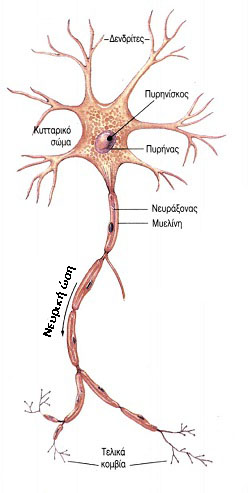
\includegraphics[width=0.4\textwidth]{nevronas}
    \caption{Σχηματική Αναπαράσταση ενός Νευρικού Κυττάρου}
    \label{fig:Neuron Cell}
\end{figure}

Το αν ένα νευρικό κύτταρο θα εκπέμψει ένα ηλεκτρικό σήμα εξαρτάται από τα εισερχόμενα ηλεκτρικά σήματα. Κάποια από αυτά παράγουν μία παρεμποδιστική δράση και τείνουν να εμποδίσουν την εκπομπή του σήματος. Κάποια άλλα δρουν διεγερτικά και προάγουν την εκπομπή του ηλεκτρικού σήματος. Τελικά η ικανότητα του κάθε νευρικού κυττάρου να επεξεργάζεται δεδομένα βασίζεται στον τύπο (παρεμποδιστικό ή διεγετρικό) και στην δύναμη των συναπτικών συνδέσεων με άλλους νευρώνες.\\

Αυτού του είδους αρχιτεκτονική και στυλ επεξαργασίας δεδομένων επιθυμούμε να ενσωματώσουμε στα τεχνητά νευρωνικά δίκτυα. Το τεχνητό ισοδύναμο των βιολογικών νευρώνων είναι οι κόμβοι που εμφανίστηκαν στον αρχικό ορισμό του νευρωνικού δικτύου. Οι συνάψεις μοντελοποιούνται με έναν πραγματικό αριθμό, το \textit{βάρος} (weight), έτσι ώστε κάθε είσοδος να πολλαπλασιάζεται με ένα βάρος πριν εισέλθει στο τεχνητό ισοδύναμο με το κυρίως σώμα του νευρικού κυττάρου. Τα σταθμισμένα σήματα εισόδου αθροίζονται ακρίβως όπως γνωρίζουμε ότι αθροίζονται οι πραγματικοί αριθμοί και στην συνέχεια επεξεργάζονται από ειδικές συναρτήσεις, οι οποίες δίνουν το όριο με βάση το οποίο το κύτταρο αποφασίζει αν θα εκπέμψει το ηλεκτρικό του σήμα ή όχι.


\subsection{Η μαθηματική δομή ενός Νευρωνικού Δικτύου}


Η μαθηματική μοντελοποίηση ενός νευρωνικού δικτύου γίνεται με ένα \textit{συνεκτικό κατευθυνόμενο γράφημα} (connected oriented graph). Αποτελείται δηλαδή από κόμβους (nodes), οι οποίοι καλούνται \textit{νευρώνες} (neurons) και από \textit{ακμές} (edges), οι οποίες συνδέουν τους νευρώνες μεταξύ τους. Η έννοια του συνεκτικού γραφήματος σημαίνει ότι κάθε νευρώνας θα πρέπει να συνδέεται με τουλάχιστον έναν άλλο νευρώνα μέσω μίας ακμής. Οι νευρώνες δεν τοποθετούνται τυχαία στο γράφημα αλλά έχουν μία συγκεκριμένη \textit{δομή}. Πιο συγκεκριμένα, οι κόμβοι του γραφήματος κατανέμονται στα λεγόμενα \textit{στρώματα} (layers) του δικτύου. Ένα τέτοιο στρώμα αποτελείται από κόμβους οι οποίοι \textit{δεν επικοινωνούν μεταξύ τους} (δηλαδή δεν συνδέονται με ακμές) αλλά δέχονται πληροφορία από προηγούμενα στρώματα. Μπορούμε να θεωρήσουμε ένα στρώμα του νευρωνικού δικτύου με $n$ νευρώνες ώς ένα διάνυσμα του $\mathbb{R}^n$. \\
Σε ένα νευρωνικό δίκτυο μπορούμε να διακρίνουμε τρία είδη στρωμάτων \cite{neuralnets3}.\\

\textit{Στρώμα Εισόδου} (Input Layer) : Το στρώμα αυτό αποτελεί την είσοδο του νευρωνικού δικτύου, με την έννοια ότι στο στρώμα αυτό τοποθετούνται τα δεδομένα προς εκπαίδευση. Τα δεδομένα αυτά, τα οποία μπορεί να προέρχονται από κάποια βάση δεδομένων (φωτογραφίες, κομμάτια ήχου κ.α.) ή ακόμη και να αποτελούν συναρτήσεις, προωθούνται στα επόμενα στρώματα του δικτύου με σκοπό να αρχίσει η εκπαίδευσή τους.\\

\textit{Κρυφά Στρώματα} (Hidden Layers) : Τα στρώματα αυτά αποτελούν την καρδιά ενός νευρωνικού δικτύου καθώς σε αυτά γίνεται το μεγαλύτερο μέρος της εκπαίδευσης. Κάθε νευρώνας ενός κρυφού στρώματος συμβολίζει μία \textit{συνάρτηση ενεργοποίησης} (activation function), οι οποίες θα αναλυθούν στην συνέχεια. Κάθε ακμή συμβολίζει το σήμα που μεταδίδεται από έναν νευρώνα στον επόμενο. Ο αριθμός των κρυφών στρωμάτων και ο αριθμός των νευρώνων σε κάθε κρυφό στρώμα αποτελεί θέμα κυρίως εμπειρικό και δεν υπάρχει ακόμη ιδιαίτερα κατατοπιστική μεθοδολογία για τον προσδιορισμό ενός βέλτιστου αριθμού κρυφών στρωμάτων και νευρώνων.\\

\textit{Στρώμα Εξόδου} (Output Layer) : Στο στρώμα αυτό εισέρχονται τα εκπαιδευμένα δεδομένα που έχουν εξέλθει από το τελευταίο κρυφό στρώμα. Ο αριθμός των νευρώνων σε αυτό το στρώμα εξαρτάται από το εκάστοτε πρόβλημα.\\

\begin{figure}[h]
    \centering
    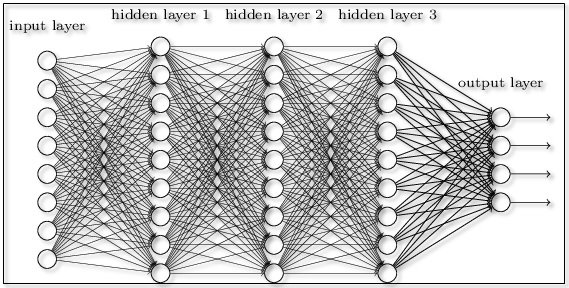
\includegraphics[width=0.6\textwidth]{NN}
    \caption{Αναπαράσταση ενός νευρωνικού δικτύου με τρία κρυφά στρώματα}
    \label{fig:Neural Net}
\end{figure}


Εφόσον το νευρωνικό δίκτυο σχηματίσει επιτυχώς το στρώμα εξόδου, σκοπός μας είναι να \textit{συγκρίνουμε} τα δεδομένα του στρώματος εξόδου με τις προβλέψεις μας, δηλαδή με τις επιθυμητές τιμές. Αυτό επιτυγχάνεται με τη βοήθεια μιας ειδικής \textit{συνάρτησης κόστους} (Loss Function). Η συνάρτηση αυτή μας βοηθά να ποσοτικοποιήσουμε το σφάλμα ή την απόκλιση των δεδομένων του στρώματος εξόδου σε σχέση με τις επιθυμητές τιμές. Στόχος μας προφανώς είναι να ελαχιστοποιήσουμε το σφάλμα αυτό και σε αυτήν την ελαχιστοποίηση συνίσταται η \textit{εκπαίδευση} ενός νευρωνικού δικτύου, όπως θα αναλυθεί παρακάτω.

\subsection{Εκπαίδευση ενός Νευρωνικού Δικτύου}
Με τον όρο \textit{εκπαίδευση} του νευρωνικού δικτύου εννοούμε την \textit{ρύθμιση} ή \textit{προσαρμογή} των ειδικών \textit{παραμέτρων} του δικτύου, που ονομάζονται \textit{βάρη} (weights) και \textit{μεροληψίες} (στο εξής bias). Οι παράμετροι αυτοί αρχικοποιούνται τυχαία και με βάση τον αλγόριθμο που θα περιγραφεί παρακάτω προσπαθούμε να βρούμε τις βέλτιστες δυνατές τιμές αυτών.\\

Ας υποθέσουμε ότι έχουμε ένα νευρωνικό δίκτυο με $N$ κρυφά στρώματα, δηλαδή συνολικά το δίκτυο έχει $N+2$ στρώματα. Σε κάθε στρώμα αντιστοιχίζονται δύο \textit{πίνακες}, ο πίνακας των βαρών, $\textbf{W}_{jk} ^l$ και ο πίνακας των biases, $\textbf{b}^{l}_{j}$. Με $\textbf{W}_{jk} ^l$ συμβολίζουμε το βάρος για την σύνδεση του $k$-οστού νευρώνα του (l-1)-οστού στρώματος στον $j$-οστό νευρώνα του $l$-οστού στρώματος . Ως σύμβαση το στρώμα εισόδου θα έχει $l = 0$,  τα κρυφά στρώματα θα έχουν $l = 1, \dots , N$ ενώ το στρώμα εξόδου θα έχει $l=L$. Κάθε στοιχείο του πίνακα των βαρών μεταφράζεται ως η συνεισφορά ενός συγκεκριμένου νευρώνα στο υπολογισμό της εξόδου του επόμενου νευρώνα με τον οποίο συνδέεται. Το μοναδικό στρώμα για το οποίο δεν έχει νόημα να αντιστοιχίσουμε πίνακα βαρών είναι το στρώμα εξόδου αφού η προώθηση τελειώνει εκεί. Με $\textbf{b}^{l}_{j}$ συμβολίζουμε το bias του $j$-οστού νευρώνα στο $l$-οστό στρώμα. Η διαστάσεις του πίνακα των βαρών και των biases καθορίζονται από την διάσταση (τον αριθμό των νευρώνων) των στρωμάτων στα οποία αναφέρεται. Ένας πίνακας με biases αντιστοιχίζεται σε όλα τα στρώματα εκτός από το στρώμα εισόδου και έχει διάσταση $1 \times n$, όπου n ο αριθμός των νευρώνων του αντίστοιχου στρώματος. \\

Για παράδειγμα ας υποθέσουμε ότι το στρώμα εισόδου ενός νευρωνικού δικτύου έχει 5 νευρώνες και το αμέσως επόμενο στρώμα, δηλαδή το πρώτο κρυφό στρώμα, έχει 10 νευρώνες (νούμερα πάρα πολύ μικρά για ένα τυπικό νευρωνικό δίκτυο!). Τότε ο πίνακας  $\textbf{W}_{jk} ^1$ είναι ο πίνακας των βαρών που δίνει την συνεισφορά των στοιχείων του στρώματος εισόδου στον υπολογισμό της εξόδου των στοιχείων του πρώτου κρυφού στρώματος. Η διάσταση του πίνακα αυτού είναι $5 \times 10 = 50$, περιέχει δηλαδή 50 βάρη. Άρα προς το παρόν έχουμε 50 μεταβλητές. Επίσης για το πρώτο κρυφό στρώμα έχουμε επίσης 10 biases, άρα συνολικά 60 μεταβλητές. Τέλος ας υποθέσουμε ότι το νευρωνικό μας δίκτυο έχει μόνο ένα κρυφό στρώμα και το στρώμα εξόδου έχει 3 νευρώνες. Άρα ο πίνακας $\textbf{W}_{jk} ^{L}$ θα έχει 30 βάρη και επίσης στο στρώμα εξόδου θα αντιστοιχισθούν 3 βάρη. Συνολικά δηλαδή το νευρωνικό μας δίκτυο αποτελεί μία συνάρτηση $60 + 30 + 3 = 93$ μεταβλητών, οι οποίες όχι μόνο πρέπει να υπολογισθούν αλλά να βρεθεί και η βέλτιστη τιμή αυτών. Όπως είναι προφανές, ακόμα και για ένα πολύ απλό νευρωνικό δίκτυο, η εκπαίδευση αποτελεί μία πολύ περίπλοκη διαδικασία βελτιστοποίησης μιας συνάρτησης πάρα πολλών μεταβλητών. \\

Περιληπτικά η μεθοδολογία της εκπαίδευσης είναι η εξής: Η πληροφορία των δεδομένων εισόδου \textit{προωθείται} μέσα στο νευρωνικό δίκτυο και επεξεργάζεται μέσω της διαδικασίας \textit{feed forward}. Μόλις η πληροφορία φθάσει στο στρώμα εξόδου συγκρίνεται με τις αντίστοιχες επιθυμητές τιμές (που μπορεί να είναι για παράδειγμα πειραματικά δεδομένα ή δικές μας προβλέψεις). Η σύγκριση αυτή γίνεται με την βοήθεια μιας συνάρτησης κόστους. Πιο συγκεκριμένα λαμβάνεται η \textit{μερική παράγωγος} της συνάρτησης κόστους ως προς όλες τις παραμέτρους του στρώματος εξόδου (βάρη και biases). Ανάλογα με το πρόσημο της κάθε μερικής παραγώγου το νευρωνικό δίκτυο καταλαβαίνει με ποιον τρόπο θα πρέπει να αλλάξει η κάθε παράμετρος \textit{προκειμένου να ελαχιστοποιηθεί η συνάρτηση κόστους} που έχουμε επιβάλλει. Στην συνέχεια η πληροφορία αυτή \textit{διαδίδεται προς τα πίσω} μέσω της διαδικασίας της \textit{Προς-τα-πίσω διάδοσης} (Back-propagation). Η διαδικασία αυτή αποτελεί μία συνεχόμενη εφαρμογή του \textit{κανόνα της αλυσίδας} και βοηθά το νευρωνικό δίκτυο να καταλάβει με ποιον τρόπο πρέπει να αλλάξουν όλες οι παράμετροι όλων των υπόλοιπων στρωμάτων του δικτύου. Μία επανάληψη του κύκλου που αποτελείται από μία διαδικασία feed-forward και μία διαδικασία back-propagation καλείται \textit{εποχή} (epoche). Το νευρωνικό δίκτυο διανύει όσες εποχές χρειάζεται έτσι ώστε να βρεθεί ένα ελάχιστο (το οποίο τις περισσότερες φορές είναι τοπικό και πάρα πολύ σπάνια ολικό) της συνάρτησεις κόστους. \\

Συνεχίζουμε παρουσιάζοντας το πρώτο στάδιο της εκπαίδευσης ενός νευρωνικού δικτύου, την προώθηση της πληροφορίας.\\


\subsection{Προώθηση (Feed Forward)}  

Το πρώτο στάδιο της εκπαίδευσης ενός νευρωνικού δικτύου είναι η εισαγωγή των δεδομένων μας σε αυτό, μέσω του στρώματος εισόδου, και η επεξεργασία τους από τα κρυφά στρώματα. Η διαδικασία είναι η εξής \cite{neuralnets2}: \\
Ένα δεδομένο $\textbf{x}_k$ που εξέρχεται από έναν νευρώνα του στρώματος εισόδου πολλαπλασιάζεται με το στοιχείο $\textbf{W}_{jk} ^{1}$ και στο αποτέλεσμα προστίθεται το αντίστοιχο βάρος  $\textbf{b}^{1}_{k}$. Σχηματίζεται έτσι η ποσότητα:
\begin{align*}
\psi_{jk} ^ {1}   =  \textbf{W}_{jk} ^{1} \textbf{x}_k + \textbf{b}_k ^{1}
\end{align*}
 $\forall k = 1, 2, \dots, Ν$ όπου Ν ο αριθμός των νευρώνων του στρώματος εισόδου. Στην συνέχεια αθροίζουμε πάνω στον δείκτη $k$ και παίρνουμε έτσι ένα \textit{σταθμισμένο άθροισμα} των δεδομένων εισόδου. Το άθροισμα αυτό θα αποτελέσει την είσοδο του $j$ νευρώνα του πρώτου κρυφού στρώματος. Όπως προαναφέρθηκε, κάθε νευρώνας ενός κρυφού στρώματος αντιπροσωπεύει μία συνάρτηση ενεργοποίησης. Συνεπώς η έξοδος του $j$ νευρώνα του πρώτου κρυφού στρώματος θα είναι το {κανονικοποιημένο σταθμισμένο άθροισμα}:
\begin{equation}
\displaystyle \alpha^{j}_{1} = \sigma \left( \sum_{k} \psi_{jk} ^ 1 \right)  =  \sigma \left(\sum_{k} \textbf{W}_{jk} ^{1} \textbf{x}_k + \textbf{b}_{k}^{1}  \right) = \sigma \left( z_{j}^{1} \right)
\end{equation}
Από το σημείο αυτό και μέχρι το στρώμα εξόδου η διαδικασία συνεχίζεται με παρόμοιο τρόπο. Στο πρώτo κρυφό στρώμα θα αντιστοιχισθούν οι πίνακες βαρών και biases. Για κάθε νευρώνα του πρώτου κρυφού στρώματος θα σχηματισθεί το σταθμισμένο άθροισμα και τελικά το άθροισμα αυτό θα περάσει σε όλους του νευρώνες του δεύτερου κρυφού στρώματος, όπου και θα δράσει η αντίστοιχη συνάρτηση ενεργοποίησης. Η έξοδος του κάθε νευρώνα του τελευταίου κρυφού στρώματος θα πολλαπλασιασθεί με το αντίστοιχο στοιχείο του τελευταίου πίνακα βαρών, θα προστεθεί το τελευταίο διάνυσμα biases και το τελικό αυτό αποτέλεσμα θα αποτελέσει το στρώμα εξόδου. Παίρνουμε έτσι τον αναδρομικό τύπο των τιμών ενεργοποίησης\\
\begin{equation}
\alpha_{j}^{l} = \sigma (z_{j}^{l}) = \sigma \left( \sum_{k} W^{l}_{jk} \alpha^{l-1}_{k} + b_{j}^{l} \right)
\end{equation}

Η ποσότητα $\alpha_{j} ^ {l}$ ονομάζεται \textit{τιμή ενεργοποίησης} (activation value). Το παραπάνω άθροισμα είναι πάνω σε όλους τους νευρώνες του $(l-1)$-οστού στρώματος.

Συνεχίζουμε την διερεύνηση της εκπαίδευσης ενός νευρωνικού δικτύου με μία μικρή παράκαμψη. Όπως αναφέρθηκε προηγουμένως τα δεδομένα του δικτύου επεξεργάζονται με την βοήθεια των λεγόμενων συναρτήσεων ενεργοποίησης. Θα εξετάσουμε τις πιθανές υποψήφιες κλάσσεις τέτοιων συναρτήσεων, ποιες είναι κατάλληλες και ποιες όχι.

\subsection{Συναρτήσεις Ενεργοποίησης}

Οι συναρτήσεις ενεργοποίησης είναι ο τρόπος με τον οποίο η πληροφορία των σημάτων εισόδου περνούν από τον έναν νευρώνα στον επόμενο. Σηματοδοτούν δηλαδή πότε ένας νευρώνας θα "ενεργοποιηθεί" και θα μεταβιβάσει την εκάστοτε πληροφορία. Υπάρχουν πολλές υποψήφιες επιλογές συναρτήσεων ενεργοποίησης και η επιλογή της "καταλληλότερης" συνάρτησης για τον κάθε νευρώνα (η συνηθέστερα για το κάθε κρυφό στρώμα) είναι ως επί το πλείστον εμπειρική και αποτελεί πηγή πολλών ερευνητικών δυνατοτήτων. Για να καταλάβουμε τί είδους συναρτήσεις είναι κατάλληλες για την μεταφορά πληροφορίας μεταξύ των νευρώνων μπορούμε να ξεκινήσουμε μελετώντας ποιες συναρτήσεις \textit{δεν είναι κατάλληληλες} για αυτόν τον σκοπό.\\

Η μελέτη των συναρτήσεων ενεργοποίησης ξεκίνησε με την εξής απλή σκέψη: Εφόσον ένας νευρώνας είτε θα μεταβιβάσει είτε δεν θα μεταβιβάσει την πληροφορία στον επόμενο νευρώνα, τι πιο φυσικό από το να χρησιμοποιήσουμε την \textit{βηματική συνάρτηση} (step function): 

\[ 
\ \sigma(x) = \left\{
\begin{array}{ll}
      1 & , x > 0 \\
      0 & , x < 0 \\
\end{array} 
\right. 
\]

Παρόλο που η παραπάνω συνάρτηση φαίνεται διαισθητικά σωστή, στην πραγματικότητα εμφανίζει πολύ άσχημα αποτελέσματα στην πράξη της εκπαίδευσης των δικτύων. Αυτό οφείλεται στο γεγονός ότι ο ορισμός της παραπάνω συνάρτησης θα επιτρέψει στον νευρώνα είτε να μεταδώσει πλήρως την πληροφορία του είτε καθόλου, ενεργεί δηλαδή με δυαδικό τρόπο. Στην πράξη παρόλα αυτά μία καλή εκπαίδευση θα πρέπει να περιλαμβάνει και "ποσοστά μετάδοσης" πληροφορίας. Με αυτόν τον τρόπο το δίκτυό μας έχει περισσότερους βαθμούς ελευθερίας για να προσαρμόσει τις προς προσδιορισμό παραμέτρους του και αυτό προσφέρει μεγαλύτερη ευρωστία στην αρχιτεκτονική του. \\

Συνεπώς θα πρέπει να επιλέξουμε μία συνάρτηση που να δίνει και ενδιάμεσες τιμές ενεργοποίησης. Η πρώτη σκέψη είναι μία γραμμική συνάρτηση:
\begin{align*}
\sigma (x) = \alpha x
\end{align*}

Μια συνάρτηση τέτοιας μορφής μπορεί να δώσει όντως μια μεγάλη ποικιλία τιμών ενεργοποίησης, οι οποίες τιμές είναι ανάλογες της εκάστοτε εισόδου. Παρόλα αυτά οι γραμμικές συναρτήσεις έχουν δύο σοβαρά μειονεκτήματα. Το πρώτο είναι το γεγονός ότι έχουν \textit{σταθερή βαθμίδα} (ή \textit{κλίση}). Αυτό σημαίνει ότι αν υπάρχει σφάλμα στην πρόβλεψη, δηλαδή η έξοδος του νευρωνικού δικτύου διαφέρει από την επιθυμητή τιμή, τότε η διόρθωση και οι αλλαγές που θα γίνονται με την προς-τα-πίσω μετάδοση θα είναι σταθερές και δεν θα εξαρτώνται από το σφάλμα αυτό. Το δεύτερο μειονέκτημα δεν είναι τόσο προφανές. Αν όλες οι συναρτήσεις ενεργοποίησης επιλεγούν γραμμικές τότε η τελική έξοδος του νευρωνικού δικτύου θα είναι και αυτή μία γραμμική συνάρτηση της εισόδου. Στην ουσία το σύνολο του νευρωνικού δικτύου (που μπορεί να περιέχει μέχρι και δεκάδες κρυφά στρώματα!) θα είναι ισοδύναμο με ένα νευρωνικό δίκτυο με ένα μόνο κρυφό στρώμα, εφόσον η σύνθεση γραμμικών συναρτήσεων είναι μία επίσης γραμμική συνάρτηση. Αυτό στην πράξη σημαίνει χειρότερη εκπαίδευση.\\

Το επόμενο βήμα δεν είναι ιδιαίτερα προφανές. Χρειαζόμαστε μία συνάρτηση που να έχει τουλάχιστον τις εξής ιδιότητες:
\begin{itemize}
  \item Μη-γραμμική
  \item Φραγμένη (προτιμέστερα μεταξύ του 0 και του 1, χωρίς να έχει ιδιαίτερη σημασία)
  \item Να είναι τουλάχιστον μια φορά συνεχώς παραγωγίσιμη 
\end{itemize}

Μία πολύ καλή υποψήφια συνάρτηση είναι η λεγόμενη \textit{λογιστική συνάρτηση}:
\begin{align*}
\sigma(x) = \frac{1}{1+e^{-x}}
\end{align*}

\begin{figure}[H]
    \centering
    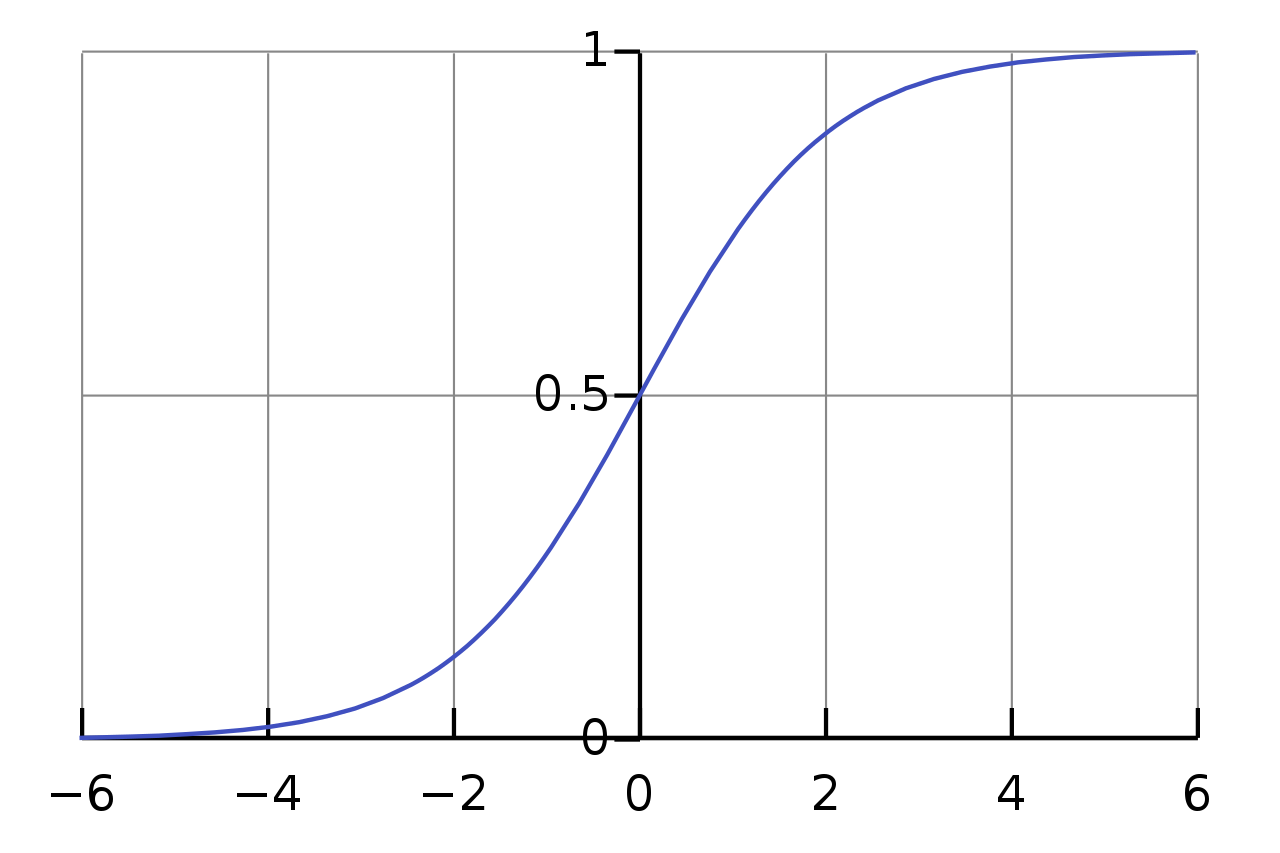
\includegraphics[width=0.7\textwidth]{logcurve}
    \caption{Γραφική παράσταση της λογιστικής συνάρτησης}
    \label{fig:logistic curve}
\end{figure}

Η παραπάνω συνάρτηση έχει όλες τις παραπάνω επιθυμητές ιδιότητες συν άλλη μία η οποία δεν είναι άμεσα προφανής. H λογιστική συνάρτηση έχει κλίση που δίνεται από τον τύπο:
\begin{align*}
\nabla \sigma(x) = \frac{e^x}{(e^x + 1)^2}
\end{align*}

 Στο διάστημα [-2,2] η κλίση της λογιστικής συνάρτησης είναι αρκετά μεγάλη, όπως φαίνεται και από την γραφική της παράσταση. Μεγάλη κλίση σημαίνει πως μικρές μεταβολές των μεταβλητών εισόδου (μικρά Δx) οδηγούν σε μεγάλες μεταβολές των μεταβλητών εξόδου. Υπάρχει δηλαδή αρκετά μεγάλη ευαισθησία σε μικρές διαταραχές του σήματος που εισέρχεται στον νευρώνα και αυτό συνεπάγεται πιο αποδοτική εκπαίδευση με την χρήση της προς-τα-πίσω μετάδοσης. \\

Η λογιστική συνάρτηση είναι όντως μία από τις ευρέως χρησιμοποιούμενες συναρτήσεις ενεργοποίησης στην τεχνολογία των νευρωνικών δικτύων λόγω των προαναφερθέντων ιδιοτήτων της. Στο σημείο αυτό όμως θα πρέπει να αναφερθεί και το μοναδικό μειονέκτημα της εν λόγω συνάρτησης που οφείλεται στην ίδια την φύση της. Παρατηρούμε από την παραπάνω γραφική παράσταση ότι στο σύνολο $[-\infty,-2] \cup [2, +\infty]$ η κλίση της λογιστικής συνάρτησης πρακτικά μηδενίζεται (η συνάρτηση τείνει να γίνει οριζόντια). Παρουσιάζεται δηλαδή το φαινόμενο των \textit{εξαφανισμένων βαθμίδων} (vanishing gradients). Πολύ μικρές βαθμίδες στα διαστήματα αυτά σημαίνει πως μόλις η εκπαίδευση μας οδηγήσει στα "άκρα" της συνάρτησης τότε η εκπαίδευση επιβραδύνεται με πολύ μεγάλο ρυθμό και πρακτικά σταματά.\\

Το επόμενο βήμα αποτελεί μία βελτίωση της λογιστικής συνάρτησης και ονομάζεται \textit{υπερβολική εφαπτομένη}:
\begin{align*}
\sigma(x) = \tanh{x} = \frac{e^x - e^{-x}}{e^x + e^{-x}}
\end{align*}

\begin{figure}[H]
    \centering
    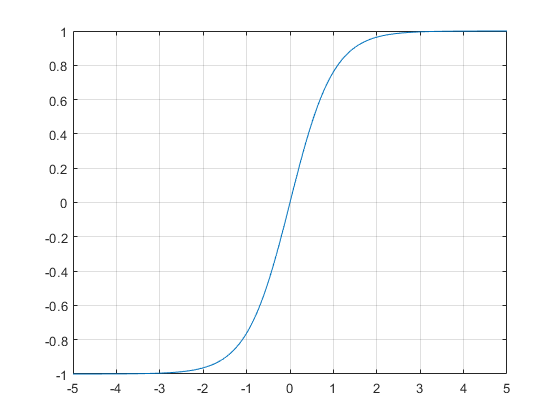
\includegraphics[width=0.7\textwidth]{tanh}
    \caption{Γραφική παράσταση της υπερβολικής εφαπτομένης}
    \label{fig:tanh curve}
\end{figure}

Συγκρίνοντας τις κλίσεις της λογιστικής συνάρτησης και της υπερβολικής εφαπτομένης παρατηρούμε ότι στο κοινό διάστημα [-2,2] η υπερβολική εφαπτομένη έχει μεγαλύτερη κλίση. Κατά τ'άλλα παρουσιάζει τα ίδια μειονεκτήματα και πλεονεκτήματα με την λογιστική συνάρτηση. Η επιλογή ανάμεσα στις δύο αυτές συναρτήσεις εξαρτάται από το πόσο μεγάλες κλίσεις θέλουμε να επιβάλλουμε στο νευρωνικό μας δίκτυο. Αποτελεί προς το παρόν θέμα κυρίως εμπειρικό και εξαρτάται από το εκάστοτε πρόβλημα.\\

Εναλλακτικές επιλογές συναρτήσεων που παρουσιάζουν παρόμοια χαρακτηριστικά με την λογιστική συνάρτηση και την υπερβολική εφαπτομένη είναι οι εξής συναρτήσεις:
\begin{gather*}
f(x) = \arctan{x} \\
f(x) = \frac{x}{1+\abs{x}}\\
f(x) = \frac{x}{\sqrt{1+\alpha x^2}}
\end{gather*}

Όλες οι παραπάνω μη-γραμμικές συναρτήσεις ανήκουν στην ειδικότερη κατηγορία των \textit{σιγμοειδών} συναρτήσεων (sigmoid functions) και είναι η πιο ευρέως χρησιμοποιούμενη κατηγορία συναρτήσεων ενεργοποίησης στα νευρωνικά δίκτυα λόγω των ιδιοτήτων τους. Τα τελευταία χρόνια όμως έχει τεθεί σε εφαρμογή μια συνάρτηση που δεν είναι σιγμοειδής και ονομάζεται \textbf{ReLU} (Rectified Linear Unit). Δίνεται από την σχέση: 
\[ 
\ R(x) = \left\{
\begin{array}{ll}
      x & , x > 0 \\
      0 & , x < 0 \\
\end{array} 
\right. 
\]

Η ReLU μπορεί να ορισθεί και ως R(x) = $\max{(0,x)}$. Παρά το γεγονός ότι με μία πρώτη ματιά η ReLU φαίνεται γραμμική, στην πραγματικότητα δεν είναι. Μια γραμμική απεικόνιση $T : \mathbb{R} \rightarrow \mathbb{R}$ ικανοποιεί τις εξής σχέσεις:
\begin{gather*}
T(x + y) = T(x) + T(y)\\
T(\lambda x) = \lambda x
\end{gather*}

Είναι προφανές ότι η ReLU δεν ικανοποιεί την πρώτη συνθήκη των γραμμικών συναρτήσεων. Ως παράδειγμα έχουμε:\\
$ R(1) = \max{(0,1)} = 1$.
Όμως $1 = 2 - 1$ και αν υποθέσουμε ότι η ReLU είναι γραμμική τότε θα ισχύει ότι:
$R(2 -1) = R(2) + R(-1) = 2 = R(1) = 1$ καί έτσι καταλήγουμε σε άτοπο και άρα στο συμπέρασμα ότι η ReLU δεν είναι γραμμική.

\begin{figure}[H]
    \centering
    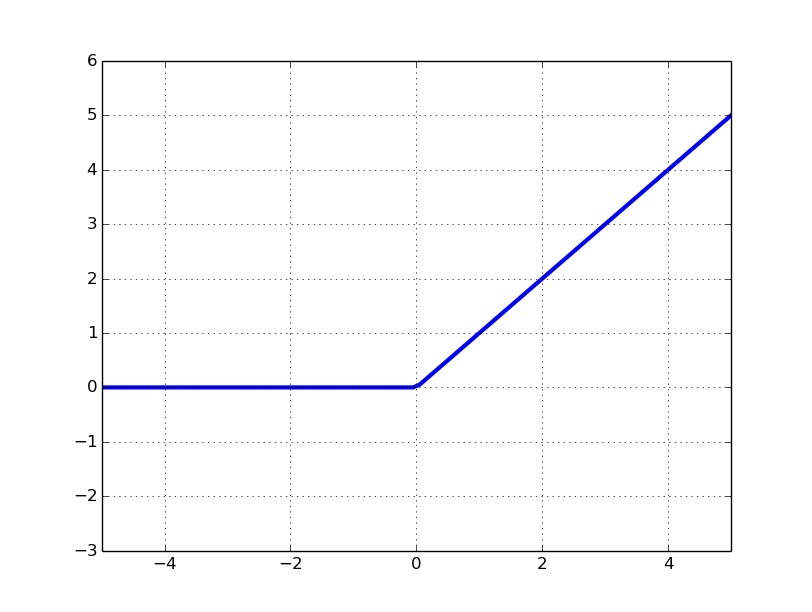
\includegraphics[width=0.7\textwidth]{relu}
    \caption{Γραφική παράσταση της ReLU}
    \label{fig:RELU curve}
\end{figure}

Ένα ενδιαφέρον χαρακτηριστικό της ReLU είναι ότι μπορεί να δράσει πολύ καλά ως συναρτησιακός προσεγγιστής, με την έννοια ότι μπορούμε να προσεγγίσουμε όσο καλά θέλουμε μία συνεχή συνάρτηση με την χρήση γραμμικού συνδυασμού συναρτήσεων ReLU. Πιο φορμαλιστικά, για κάθε $\epsilon > 0$ και για κάθε συνεχή συνάρτηση $f$ υπάρχει ένας φυσικός $Ν$, πραγματικοί αριθμοί $\alpha_i$ και συναρτήσεις ReLU ορισμένες σε κατάλληλο εκάστοτε διάστημα, ώστε :
\begin{align*}
\displaystyle \abs{f - \sum_{i=1}^{N} \alpha_i R_i(x)} < \epsilon
\end{align*}

Στις περισσότερες περιπτώσεις η ReLU χρησιμοποιείται σε συνδυασμό με άλλες συναρτήσεις ενεργοποίησης, συνήθως σιγμοειδείς. Η παρουσία της προσφέρει ένα σημαντικό πλεονέκτημα. Λόγω της μορφής της δεν επιτρέπει σε όλους τους νευρώνες να ενεργοποιηθούν. Αν φανταστούμε ένα νευρωνικό δίκτυο με εκατοντάδες ή και χιλιάδες νευρώνες τότε προφανώς ο υπολογιστικός χρόνος της εκπαίδευσης μπορεί να είναι πολύ μεγάλος για να είναι πρακτικός. Η χρήση της ReLU λοιπόν μας βοηθά να δημιουργήσουμε ένα νευρωνικό δίκτυο πιο αραιό και ανάλαφρο και έτσι να εξοικονομήσουμε πολύτιμο υπολογιστικό χρόνο. Αυτό είναι το μεγάλο πλεονέκτημά της. Το πρόβλημα που δημιουργεί είναι προφανές στο σημείο αυτό και είναι η μηδενική κλίση (δηλαδή τερματισμός της εκπαίδευσης) για αρνητικές τιμές εισόδου. Το πρόβλημα αυτό λύνεται με μικρές παραλλαγές της ReLU που παίρνουν την μορφή:
\[ 
\ R_\epsilon(x) = \left\{
\begin{array}{ll}
      x & , x > 0 \\
      \epsilon x & , x < 0 \\
\end{array} 
\right. 
\]
όπου $\epsilon << 1$. Η μικρή παράμετρος $\epsilon$ μπαίνει έτσι ώστε να υπάρχει μη-μηδενική κλίση για αρνητικές τιμές εισόδου. Τέτοιες παραλλαγές της ReLU είναι γνωστές ως \textbf{Leaky ReLU}.\\

\subsection{Συναρτήσεις Κόστους}
Η ανάγκη για την ύπαρξη μίας συνάρτησης κόστους στο νευρωνικό δίκτυο έγκειται στο γεγονός ότι χρειαζόμαστε ένα κριτήριο με βάση το οποίο θα γίνει η εκπαίδευση του δικτύου. Οι συναρτήσεις κόστους μας βοηθούν να συγκρίνουμε τις τιμές του στρώματος εξόδου με τις επιθυμητές τιμές (προβλέψεις ή πειραματικά δεδομένα). Είναι δηλαδή ο τρόπος με τον οποίο βοηθούμε τον υπολογιστή να καταλάβει αν η διαδικασία της προώθησης ήταν επιτυχής. Για λόγους που δεν είναι άμεσα προφανείς και σχετίζονται με την διαδικασία του back-propagation οι συναρτήσεις κόστους πρέπει να πληρούν τις δύο εξής προϋποθέσεις \cite{neuralnets3}:\\
\begin{itemize}
\item Η συνάρτηση κόστους θα πρέπει να μπορεί να γραφεί ως ένας μέσος όρος $\displaystyle C = \frac{1}{n} \sum_{x} C_{x}$ συναρτήσεων κόστους για κάθε μεμονωμένο αντικείμενο εκπαίδευσης, $x$. Ο λόγος που χρειαζόμαστε αυτήν την προϋπόθεση είναι επειδή στον αλγόριθμο back-propagation απαιτείται ο υπολογισμός μερικών παραγώγων ως προς όλα τα αντικείμενα προς εκπαίδευση.\\
\item Η συνάρτηση κόστους θα πρέπει να μπορεί να γραφτεί συναρτήσει των εξόδων του νευρωνικού δικτύου $C = C(\alpha^{l})$
\end{itemize}


Μερικές από τις ευρέως χρησιμοποιούμενες συναρτήσεις κόστους είναι οι εξής:\\

\textbf{Συνάρτηση μέσου τετραγωνικού σφάλματος} (Mean Square Error Function):
\begin{align*}
\displaystyle C = \frac{1}{n} \sum_{i=1}^{n} (y_i - \hat{y}_i)^2
\end{align*}
όπου $y_i$ οι τιμές του στρώματος εξόδου του δικτύου και $\hat{y}_i$ οι προβλέψεις μας με τις οποίες τις συγκρίνουμε. Η συνάρτηση αυτή χρησιμοποιείται ευρέως σε προβλήματα παλινδρόμησης (regression) όμως έχει ένα σοβαρό πρόβλημα. Σε περίπτωση που υπάρχουν δεδομένα (παρατηρούμενες τιμές) που απέχουν πολύ από όλα τα υπόλοιπα, τα λεγόμενα outliers, τότε η εφαρμογή της συνάρτησης τετραγωνικού σφάλματος μπορεί να έχει πολύ μεγάλα σφάλματα στους υπολογισμούς. Για τον σκοπό αυτό επινοήθηκε η συνάρτηση σφάλματος κατά Huber. \\


\textbf{Συνάρτηση Huber} (Huber Loss):
\[ 
\ C = \left\{
\begin{array}{ll}
    \displaystyle \frac{1}{2} \sum_{i} (y_i - \hat{y}_i)^2 & , \abs{y_i - \hat{y}_i} \leq \delta \hspace{0.2cm} \forall i\\
    \displaystyle \delta \sum_{i} \abs{y_i - \hat{y}_i} - \frac{1}{2} \delta ^ 2& , αλλιως\\
\end{array} 
\right. 
\]
Η συνάρτηση Huber είναι πολύ λιγότερο ευαίσθητη σε outliers.\\

\textbf{Συνάρτηση Cross Entropy}:
\begin{align*}
\displaystyle C = -\sum_{i=1}^{n} y_i \log{\hat{y}_i}
\end{align*}
Η Cross Entropy αποτελεί μια από τις σημαντικότερες συναρτήσεις για το κλάδο τον Μαθηματικών με όνομα Θεωρία Πληροφορίας.\\

Όλες οι μορφές των παραπάνω συναρτήσεων αφορούν φυσικά διακριτό χώρο δειγματοληψίας. Αν οι κατανομές μας αποτελούν συνεχείς συναρτήσεις τότε το άθροισμα αντικαθιστάται με ολοκλήρωμα.\\

\subsection{Κανονικοποίηση Κόστους}

Η κανονικοποίηση κόστους (ή κανονικοποίηση συνάρτησης κόστους) είναι μία τεχνική που χρησιμοποιούνταν αρκετές δεκαετίες πριν την ανάπτυξη της εκπαίδευσης νευρωνικών δικτύων βάθους. Γραμμικά μοντέλα όπως η γραμμική και η λογιστική παρεμβολή δίνουν την ικανότητα εφαρμογής απλών και αποτελεσματικών τεχνικών κανονικοποίησης.\\

Οι εφαρμογές κανονικοποίησης βασίζονται στον περιορισμό των ικανοτήτων και της χωρητικότητας του μοντέλου (είτε αυτό είναι νευρωνικά δίκτυα ή κάποιου είδους παρεμβολή) προσθέτοντας μια παραμετρικοποιημένη ποινή $\Omega(\textbf{\theta})$ στην αντικειμενική συνάρτηση κόστους $\mathcal{J}$. Συμβολίζουμε την κανονικοποιημένη συνάρτηση κόστους ώς
\begin{equation}
\widetilde{\mathcal{J}} = \mathcal{J}(\textbf{\theta}; \textbf{x}, \textbf{y}) + \alpha \Omega(\textbf{\theta})
\end{equation}

όπου η πολλαπλασιαστική σταθερά $\alpha \in [0, \infty)$ είναι μία υπερπαράμετρος που σταθμίζει την σχετική συνεισφορά του όρου της ποινής, $\Omega$, στην συνάρτηση κόστους, $\mathcal{J}$. Φυσικά θέτοντας $\alpha = 0$ έχει ως αποτέλεσμα να μην έχουμε καμία κανονικοποίηση. Όσο το $\alpha$ αυξάνεται τόσο αυξάνεται και η συνεισφορά της ποινής στην αντικειμενική συνάρτηση. Όταν ο αλγόριθμος εκπαίδευσής μας προσπαθεί να ελαχιστοποιήσει την αντικειμενική συνάρτηση $\widetilde{\mathcal{J}}$, τότε θα μειώνει και την συνάρτηση $\mathcal{J}$ αλλά και μία συνάρτηση της οποίας το μέτρο θα εξαρτάται καθαρά και μόνο από τις παραμέτρους $\textbf{\theta}$. Διαφορετικές επιλογές της συνάρτησεις $\Omega$ θα έχουν φυσικά διαφορετική επίδραση στην εκπαίδευση. Στο σημείο αυτό αξίζει να σημειώσουμε ότι στις περισσότερες εφαρμογές των νευρωνικών δικτύων επιβάλλουμε ποινή μόνο στα βάρη του δικτύου και όχι στα biases \cite{costreg}. Κάθε βάρος προσδιορίζει τον τρόπο που δύο μεταβλητές αλληλεπιδρούν. Η προσαρμογή ενός βάρους λοιπόν απαιτεί την παρατήρηση και των δύο αυτών μεταβλητών σε πολλές περιστάσεις. Εν αντιθέσει, ένα bias ελέγχει μόνο μία μεταβλητή. Αυτό σημαίνει ότι δεν εισάγουμε πολύ διακύμανση αφήνοντας τα βάρη μη-κανονικοποιημένα. Για το υποκεφάλαιο αυτό θα συμβολίζουμε με $\textbf{w}$ το διάνυσμα των βαρών ενός νευρωνικού δικτύου στα οποία θα επιβάλλεται μία ποινή κανονικοποίησης και με $\textbf{\theta}$ θα συμβολίζουμε όλες τις παραμέτρους του δικτύου (όλα τα βάρη και όλα τα biases). Συνεχίζουμε με τα διάφορα είδη κανονικοποίησης ποινής.\\

\begin{itemize}
\item $\mathcal{L}^{2}$ - Κανονικοποίηση ή Κανονικοποίηση \textit{Tykhonov}
\end{itemize}

Πρόκεται δηλαδή για την $\mathcal{L}^{2}$ νόρμα του διανύσματος των βαρών στα οποία επιβάλλουμε την επιπλέον ποινή. Η ποινή κόστους τύπου $\mathcal{L}^{2}$ είναι η πιο κοινή στην πράξη. Βοηθά στο να κρατά τα βάρη πιο κοντά στο $0$ \cite{linearmodel}, όπως θα δείξει η μαθηματική ανάλυση που θα ακολουθήσει. Η συνάρτηση κανονικοποίησης $\Omega$ δίνεται από την σχέση
\begin{equation}
\Omega(\textbf{\theta}) = \frac{1}{2} \norm{\textbf{w}}_{2}^{2} = \frac{1}{2} \textbf{w}^\intercal \textbf{w}
\end{equation}

Με βάση την παραπάνω ποινή η αντικειμενική συνάρτηση γράφεται ως
\begin{equation}
\widetilde{\mathcal{J}} = \mathcal{J}(\textbf{\theta}; \textbf{x}, \textbf{y}) + \frac{\alpha}{2} \textbf{w}^\intercal \textbf{w}
\end{equation}
 
Η συνάρτηση αυτή έχει βαθμίδα ως προς τα βάρη
\begin{align*}
\nabla_{\textbf{w}} \widetilde{\mathcal{J}} = \alpha \textbf{w} + \nabla_{\textbf{w}} \mathcal{J}(\textbf{\theta}; \textbf{x}, \textbf{y})
\end{align*}

Με βάση αυτήν την βαθμίδα ένα βήμα του αλγορίθμου gradient descent επικαιροποιεί το διάνυσμα των παραμέτρων $\textbf{w}$ ως εξής
\begin{align*}
\textbf{w} \leftarrow \textbf{w} - \tau (\alpha \textbf{w} + \nabla_{\textbf{w}} \mathcal{J}(\textbf{\theta}; \textbf{x}, \textbf{y}))
\end{align*}


ή, αν αναδιατάξουμε τους όρους
\begin{equation}
\textbf{w} \leftarrow (1- \tau \alpha)\textbf{w} - \tau \nabla_{\textbf{w}} \mathcal{J}(\textbf{\theta}; \textbf{x}, \textbf{y})
\end{equation}

Όπως φαίνεται από την παραπάνω εξίσωση η εισαγωγή της ποινής $\mathcal{L}^{2}$ τροποποίησε τον κανόνα επικαιροποίησης. Σε κάθε επανάληψη της διαδικασίας το διάνυσμα των βαρών συρρικνώνεται κατά έναν σταθερό παράγοντα. Στην συνέχεια θα εξετάσουμε την επίδραση της $\mathcal{L}^{2}$ ποινής κατά την διάρκεια όλης της εκπαίδευσης. Προς απλοποίηση των πράξεων του συλλογισμού που θα ακολουθήσει θα κάνουμε μία τετραγωνική προσέγγιση (στην ουσία ανάπτυγμα Taylor δευτέρου βαθμού) της μη-κανονικοποιημένης αντικειμενικής συνάρτησης $\mathcal{J}$ γύρω από το σημείο που την ελαχιστοποιεί, $\textbf{w}^{*} = \operatorname*{argmin}_{\textbf{w}} \mathcal{J}(\textbf{w})$. Γράφουμε δηλαδή
\begin{align*}
\hat{\mathcal{J}}(\textbf{w}) = \mathcal{J}(\textbf{w}^{*}) + \frac{1}{2}(\textbf{w} - \textbf{w}^{*})^\intercal \textbf{H}(\textbf{w} - \textbf{w}^{*})
\end{align*}

όπου \textbf{H} είναι ο Εσσιανός πίνακας της $\mathcal{J}$ ως προς το διάνυσμα \textbf{w} υπολογισμένος στο σημείο $\textbf{w}^{*}$. Προφανώς αν η συνάρτηση κόστους είναι τετραγωνική (που στις περισσότερες εφαρμογές είναι) τότε η προσέγγιση συμπίπτει με την ίδια την συνάρτηση. Το ελάχιστο της συνάρτησης $\hat{\mathcal{J}}(\textbf{w})$ λαμβάνεται εκεί όπου η βαθμίδα
\begin{align*}
\nabla_{\textbf{w}} \hat{\mathcal{J}}(\textbf{w}) = \textbf{H}(\textbf{w} - \textbf{w}^{*})
\end{align*}

είναι ίση με $0$. Θα συμβολίσουμε το σημειό στο οποίο ικανοποιείται η παραπάνω συνθήκη με $\hat{\textbf{w}}$. Για να εξετάσουμε την επίδραση της ποινής $\mathcal{L}^{2}$ θα πρέπει να προσθέσουμε στην παραπάνω συνθήκη και την βαθμίδα του όρου της ποινής, $\alpha \hat{\textbf{w}}$. Λαμβάνουμε έτσι
\begin{align*}
\alpha \hat{\textbf{w}} +  \textbf{H}(\textbf{w} - \textbf{w}^{*})\\
(\textbf{H} + \alpha \textbf{I})\hat{\textbf{w}} = \textbf{H}\textbf{w}^{*}\\
\hat{\textbf{w}} = (\textbf{H} + \alpha \textbf{I})^{-1} \textbf{H}\textbf{w}^{*}
\end{align*}

Παρατηρούμε ότι καθώς $\alpha \rightarrow 0$, $\hat{\textbf{w}} \rightarrow \textbf{w}^{*}$. Επειδή ο πίνακας \textbf{H} είναι πραγματικός και συμμετρικός μπορούμε να τον γράψουμε ως γινόμενο ενός διαγώνιου πίνακα \textbf{\Lambda} και έναν πίνακα \textbf{Q} που αποτελείται από μία ορθοκανονική βάση ιδιοδιανυσμάτων, ώστε $\textbf{H} = \textbf{Q} \textbf{\Lambda} \textbf{Q} ^ \intercal$ \cite{costreg}. Με βάση αυτή την αποσύνθεση λαμβάνουμε
\begin{align*}
\hat{\textbf{w}} = (\textbf{Q} \textbf{\Lambda} \textbf{Q} ^ \intercal + \alpha \textbf{I})^{-1} \textbf{Q} \textbf{\Lambda} \textbf{Q} ^ \intercal \textbf{w}^{*}\\
= (\textbf{Q}(\textbf{\Lambda} + \alpha \textbf{I})\textbf{Q}^ \intercal)^{-1} \textbf{Q} \textbf{\Lambda} \textbf{Q} ^ \intercal \textbf{w}^{*}\\
= \textbf{Q}(\textbf{\Lambda} + \alpha \textbf{I})^{-1} \textbf{\Lambda} \textbf{Q}^\intercal \textbf{w}^{*}
\end{align*}

Παραρηρούμε ότι η επίδραση της ποινής $\mathcal{L}^{2}$ είναι ακριβώς ότι ανακλιμακώνει (rescales) το διάνυσμα $\textbf{w}^{*}$ κατά μήκος των αξόνων που ορίζονται από τα ιδιοδιανύσματα του πίνακα \textbf{H}. \\

Συνεχίζουμε τώρα με την ποινή τύπου $\mathcal{L}^{1}$.

\begin{itemize}
\item $\mathcal{L}^{1} - Κανονικοποίηση$
\end{itemize}
Στην περίπτωση της κανονικοποίησης τύπου $\mathcal{L}^{1}$ η συνάρτηση $\Omega$ δίνεται από την σχέση
\begin{equation}
\displaystyle \Omega(\textbf{\theta}) = \norm{\textbf{w}}_{1} = \sum_{i} |w_{i}|
\end{equation}

Πρόκειται δηλαδή για την $\mathcal{L}^{1}$ νόρμα του διανύσματος των βαρών στα οποία επιβάλλουμε την επιπλέον ποινή. Τώρα η κανονικοποιημένη αντικειμενική συνάρτηση έχει την μορφή
\begin{equation}
 \widetilde{\mathcal{J}}(\textbf{w}; \textbf{x}, \textbf{y}) = \alpha \norm{\textbf{w}}_{1} + \mathcal{J}(\textbf{w}; \textbf{x}, \textbf{y})
\end{equation}

όπου, ομοίως με πριν, η σταθερά \alpha είναι μία υπερπαράμετρος που καθορίζει το μέγεθος της επίδρασης της κανονικοποίησης. Η βαθμίδα της κανονικοποιημένης αντικειμενικής συνάρτησης είναι 
\begin{equation}
\nabla_{\textbf{w}} \widetilde{\mathcal{J}}(\textbf{w}; \textbf{x}, \textbf{y})  = \alpha sign(\textbf{w}) + \nabla_{\textbf{w}} \mathcal{J}(\textbf{w}; \textbf{x}, \textbf{y})
\end{equation}

Από την παραπάνω βαθμίδα βλέπουμε ότι η επίδραση της $\mathcal{L}^{1}$ κανονικοποίησης είναι διαφορετική από αυτήν της $\mathcal{L}^{2}$. Πιο συγκεκριμένα η συνεισφορά της κανονικοποίησης στην βαθμίδα δεν αυξομειώνεται γραμμικά με την κάθε συνιστώσα $w_{i}$. Είναι απλώς μία πολλαπλασιαστική σταθερά \alpha με πρόσημο που εξαρτάται από το $sign(w_{i})$, δηλαδή από το πρόσημο της συνιστώσας $w_{i}$. Μία συνέπεια αυτής της μορφής βαθμίδας είναι ότι μία τετραγωνική προσέγγιση της αντικειμενικής συνάρτησης δεν θα μπορεί να δώσει απαραίτητα κάποια αναλυτική λύση όπως στην περίπτωση της κανονικοποίησης $\mathcal{L}^{2}$. Ο κανόνας επικαιροποίησης του διανύσματος των βαρών θα είναι τώρα
\begin{equation}
\textbf{w} \leftarrow \textbf{w} + \tau(\alpha sign(\textbf{w}) + \nabla_{\textbf{w}} \mathcal{J}(\textbf{w}; \textbf{x}, \textbf{y}))
\end{equation}




\subsection{Κατάβαση Βαθμίδας (Gradient Descent)}

Η διαδικασία του Gradient Descent είναι ένας αλγόριθμος με τον οποίο μπορούμε να βρούμε ένα \textit{τοπικό ακρότατο} μιας πολυμεταβλητής συνάρτησης. Η ιδέα πίσω από τον αλγόριθμο είναι απλή. Ξεκινώντας από ένα αυθαίρετο σημείο πάνω στην (υπερ)επιφάνεια που ορίζει η συνάρτηση μας τότε αν θέλουμε να κάνουμε ανάβαση της επιφάνειας, δηλαδή να πάμε προς το πιο κοντινό μέγιστο, τότε θα πρέπει να ακολουθήσουμε την κατεύθυνση που ορίζει η \textit{βαθμίδα} (gradient) της συνάρτησης στο σημείο αυτό. Αυτό είναι και το φυσικό νόημα του gradient. Σε κάθε σημείο της επιφάνειας μας λέει προς τα που πρέπει να κινηθούμε έτσι ώστε να έχουμε την μεγαλύτερη αύξηση ή \textit{κλίση}. Συνεπώς, αν επιθυμούμε να κάνουμε κατάβαση της επιφάνειας τότε θα πρέπει να ακολουθήσουμε πορεία \textit{αντίθετη της βαθμίδας}. Σε ακριβώς αυτό έγκειται ο αλγόριθμος του gradient descent, δηλαδή στην επικαιροποίηση ενός τυχαίου σημείου της επιφάνειας με βήμα ανάλογο της βαθμίδας.\\

Ας υποθέσουμε λοιπόν ότι μας δίνεται ένα συνεκτικό ανοιχτό χωρίο $D \subset \mathbb{R}^d$ και μία πραγματική συνάρτηση $f \in C^1 (D)$, η οποία θα αποκαλείται \textit{αντικειμενική συνάρτηση} (objective function)
\begin{align*}
f : D \rightarrow \mathbb{R}
\end{align*}
την οποία επιθυμούμε να ελαχιστοποιήσουμε. Ψάχνουμε δηλαδή ένα $\textbf{x}^*$, τέτοιο ώστε:
\begin{align*}
\textbf{x}^* =  \operatorname*{argmin}_{\textbf{x} \in D} f(\textbf{x})
\end{align*}
Προφανώς επίσης θα ισχύει
\begin{align*}
\nabla f(\textbf{x}^*) = 0
\end{align*}

Ο αλγόριθμος απαιτεί να του ορίσουμε το αρχικό σημείο πάνω στην επιφάνεια από το οποίο θα αρχίσει η κατάβαση (ή η ανάβαση), το \textit{βήμα επικαιροποίησης} $t_k$ και ένα \textit{όριο ανοχής} (tolerance) το οποίο θα καθορίσει πότε θα σταματήσει ο αλγόριθμος. Συνοπτικά ο αλγόριθμος gradient descent φαίνεται στον παρακάτω πίνακα. \\

\begin{table}[H]
\begin{tabular}{ |p{13cm}}
 \hline
 \multicolumn{1}{|c|}{\textbf{Αλγόριθμος Gradient Descent}} \\
 \hline
1: Αρχικοποίηση τυχαίου σημείου $\textbf{x}^{(0)}$, βήματος $t_k$ και tolerance $\epsilon$ \\
2: \textbf{while} $||\nabla f(\textbf{x}^{(k)})|| \geq \epsilon$ \textbf{do} :  \\
3: $\textbf{x}^{(k+1)} = \textbf{x}^{(k)} - t_{k} \nabla f(\textbf{x}^{(k)})$\\
4: $k \leftarrow k + 1$ \\
5: \textbf{end while}  \\
6: \textbf{return} $\textbf{x}^{(k)}$\\
\hline
\end{tabular}
\caption{Αλγόριθμος Gradient Descent}
\end{table} 

Μερικά σχόλια για τον αλγόριθμο και τις παραμέτρους του. Καταρχάς ο παραπάνω αλγόριθμος αναφέρεται σε προβλήματα βελτιστοποίησης \textit{χωρίς περιορισμούς}, δηλαδή θεωρούμε ότι όλα τα σημεία του χώρου που ορίζονται από την επιφάνεια που ορίζει η αντικειμενική συνάρτηση είναι προσβάσιμα. Ο αλγόριθμος τροποποιείται για προβλήματα που περιέχουν περιορισμούς όμως έχει την ίδια επιτυχία.\\

Στο τρίτο βήμα του αλγορίθμου παρατηρούμε ότι χρησιμοποιούμε το πρόσημο "-" για να κάνουμε επικαιροποίηση του σημείου της επιφάνειας. Ο λόγος που επιλέγουμε αυτό το πρόσημο είναι ακριβώς επειδή θέλουμε να ακολουθήσουμε μία πορεία που είναι \textit{αντίθετη} της βαθμίδας, με σκοπό να οδηγηθούμε στο ελάχιστο της συνάρτησης. Αν, αντιθέτως, χρησιμοποιούσαμε το πρόσημο "+" τότε θα ακολουθούσαμε την πορεία της ίδιας της βαθμίδας και θα πηγαίναμε προς το μέγιστο της συνάρτησης. Στην περίπτωση αυτή ο αλγόριθμος λέγεται \textit{ανάβαση βαθμίδας} (Gradient Ascent).\\

Το βήμα επικαιροποίησης $t_{k}$  μπορεί να είναι είτε ένας σταθερός αριθμός είτε να εξαρτάται από το βήμα στο οποίο βρισκόμαστε. Η δεύτερη περίπτωση είναι πιο αποδοτική αν το βήμα επιλεγεί με έναν σχετικά έξυπνο τρόπο. Το κόστος φυσικά είναι αρκετά μεγαλύτεροι υπολογιστικοί χρόνοι. Η λογική πίσω από την επιλογή του βήματος είναι η σκέψη ότι θέλουμε να ελαχιστοποιεί την αντικειμενική μας συνάρτηση σε μια περιοχή του βήματος στο οποίο πρόκειται να βρεθούμε μετά από το εκάστοτε βήμα. Σε μαθηματικούς όρους, το \textit{βέλτιστο βήμα} $t_k ^ *$ θα ικανοποιεί \cite{graddes}:
\begin{align*}
t_k ^ * = \operatorname*{argmin}_{t \geq 0} f(\textbf{x}^{(k+1)}) = \operatorname*{argmin}_{t \geq 0} f(\textbf{x}^{(k)} - t \nabla f(\textbf{x}^{(k)})
\end{align*}

Φυσικά είναι εξαιρετικά λίγες οι περιπτώσεις όπου το βήμα αυτό μπορεί να υπολογισθεί αναλυτικά μιας και στις περισσότερες εφαρμογές οι αντικειμενικές συναρτήσεις είναι μέχρι και δεκάδων μεταβλητών.\\

Το όριο $\epsilon$ είναι το κριτήριο τερματισμού του αλγορίθμου και είναι ένας πραγματικός αριθμός πολύ μικρότερος της μονάδας και φυσικά θετικός. Όταν η νόρμα (δηλαδή το μέγεθος) της βαθμίδας, $||\nabla f||$, πέσει κάτω από $\epsilon$ μετά την κ-οστή επανάληψη τότε αυτό σημαίνει ότι σε περιοχή του σημείου $\textbf{x}^{(k)}$ η κλίση της συνάρτηση είναι σχεδόν μηδενική και άρα ως γνωστόν θα είμαστε πολύ κοντά στο ακρότατο. Θεωρητικά μπορούμε να προσεγγίσουμε το ακρότατο αυτό όσο καλά θέλουμε μικραίνοντας όλο και πιο πολύ το $\epsilon$.\\

Φυσικά, επειδή καταφέραμε να βρούμε έναν τρόπο να προσεγγίσουμε ένα τοπικό ακρότατο μίας συνάρτησης δεν σημαίνει ότι μπορούμε πάντα να εντοπίσουμε το \textit{ολικό ελάχιστο} μιας συνάρτησης. Στην πραγματικότητα, ο προσδιορισμός του ολικού ελαχίστου μια πολυμεταβλητής συνάρτησης είναι ένα υπέρμετρα δύσκολο μαθηματικό πρόβλημα. Για τον λόγο αυτό στις περισσότερες εφαρμογές η εύρεση ενός τοπικού ακροτάτου της αντικειμενικής μας συνάρτησης θεωρείται επιτυχία. Επίσης κρίνεται σκόπιμο να αναφερθεί ότι στην περίπτωση που η αντικειμενική μας συνάρτηση είναι κυρτή (αντ. κοίλη) τότε γνωρίζουμε από τον μαθηματικό λογισμό ότι θα παρουσιάζει μοναδικό ελάχιστο (αντ. μέγιστο). Συνεπώς στις περιπτώσεις αυτές ο αλγόριθμος gradient descent μας εγγυάται σύγκλιση αφού η βαθμίδα πάντα θα οδηγεί προς το μέγιστο ή το ελάχιστο  \\

\subsection{Σύγκλιση του αλγορίθμου Gradient Descent}
Ένα εύλογο ερώτημα που προκύπτει είναι κατά πόσο ο αλγόριθμος gradient descent δουλεύει, δηλαδή κατά πόσο συγκλίνει. Η απάντηση δεν είναι απλή και χρειαζόμαστε, μεταξύ άλλων, τον παρακάτω ορισμό:\\

\textbf{Ορισμός}: Έστω ένα κυρτό σύνολο $D \subset \mathbb{R}^d$, μία κυρτή συνάρτηση $f : D \rightarrow \mathbb{R}$. Η $f$ θα λέγεται \textbf{ισχυρώς κυρτή} (strongly convex) αν υπάρχει θετικός πραγματικός αριθμός m τέτοιος ώστε για κάθε $x,y \in D$:
\begin{align*}
\langle \nabla f(x) - \nabla f(y), x - y \rangle \geq m \parallel x - y \parallel ^ 2
\end{align*}
όπου $\parallel \cdot \parallel$ μία οποιαδήποτε νόρμα. Αποδεικνύεται \cite{graddes2} ότι η παραπάνω ανισότητα ισοδυναμεί με την ύπαρξη θετικών πραγματικών αριθμών m και M για τους οποίους ισχύει:
\begin{align*}
mI \leq \mathcal{H}_f (\textbf{x}) \leq MI
\end{align*}
όπου $\mathcal{H}_f (\textbf{x})$ ο εσσιανός πίνακας της $f$ στο \textbf{x} και I ο μοναδιαίος πίνακας. Σημειώνεται ότι για δύο πίνακες A και B ίδιων διαστάσεων $A \geq B$ σημαίνει ότι ο πίνακας Α - B είναι θετικά ημι-ορισμένος.  Μπορούμε έυκολα να δείξουμε ότι μία ισχυρώς κυρτή συνάρτηση είναι και αυστηρά κυρτή \cite{graddes2}. Παίρνοντας το ανάπτυγμα Taylor δεύτερης τάξης για την $f$ έχουμε ότι για $x,y \in D$ μπορούμε να βρούμε ένα $z \in [x, y]$ τέτοιο ώστε:
\begin{align*}
f(y) = f(x) + \nabla f(x) ^ \intercal (y - x) + \frac{1}{2} (y - x) ^ \intercal \mathcal{H}_f (y - x)
\end{align*}
και λόγω της παραπάνω διπλής ανισότητα παίρνουμε:
\begin{align*}
f(y) \geq f(x) + \nabla f(x) ^ \intercal (y - x) + \frac{m}{2} \parallel y - x \parallel ^ 2
\end{align*}
και επειδή $\frac{m}{2} \parallel y - x \parallel ^ 2 > 0$:
\begin{align*}
f(y) > f(x) + \nabla f(x) ^ \intercal (y - x)
\end{align*}
Έχοντας τώρα την ιδιότητα της ισχυρής κυρτότητας παίρνουμε το εξής θεώρημα \cite{graddes}:\\

\textbf{Θεώρημα}: Έστω $ f : D \rightarrow \mathbb{R}$ μία ισχυρώς κυρτή συνάρτηση με παραμέτρους m και Μ, όπως και στην παραπάνω διπλή ανισότητα, και $\alpha^* = \min_{\textbf{x} \in D} f(\textbf{x})$. Τότε για κάθε $\epsilon > 0$ μπορούμε να πετύχουμε $f(\textbf{x}^{(k^*)}) - \alpha^* \leq \epsilon$ μετά από $k^*$ επαναλήψεις για κάποιο $κ^*$ που ικανοποιεί:
\begin{align*}
k^* \geq \frac{\log \left( \frac{f(\textbf{x}^{(0)}) - \alpha^*}{\epsilon}\right)}{\log \left( \frac{1}{1 - \frac{m}{M}} \right)}
\end{align*}

Το παραπάνω θεώρημα μας εξασφαλίζει ότι μετά από έναν αριθμό επαναλήψεων που εξαρτάται από την φύση της ίδιας της συνάρτησης (τις σταθερές m και Μ) αλλά και από την ακρίβεια που επιθυμούμε μπορούμε να φτάσουμε όσο κοντά θέλουμε στο ακρότατο της $f$. Προφανώς όταν $\epsilon \rightarrow 0$ τότε $k^* \rightarrow +\infty$. Επίσης παρατηρούμε ότι καθώς $m \rightarrow M$ απαιτούνται όλο και λιγότερες επαναλήψεις για να συγκλίνει ο αλγόριθμος.\\

Προφανώς ο ρόλος του αλγορίθμου του gradient descent στα πλαίσια των νευρωνικών δικτύων είναι η ελαχιστοποίηση των συναρτήσεων κόστους ως προς τις παραμέτρους του δικτύου, δηλαδή τα βάρη και τα biases. Συνεπώς ένα κρίσιμο βήμα της εκπαίδευσης είναι ο υπολογισμός των βαθμίδων της συνάρτησης κόστους ως προς όλες αυτές τις παραμέτρους ξεχωριστά. Στο σημείο αυτό όμως, έχοντας αρχίσει να εφαρμόζουμε τον αλγόριθμο gradient descent, παρατηρούμε ότι παρουσιάζεται ένα μείζονος σημασίας πρόβλημα και αυτό είναι οι τεράστιοι υπολογιστικοί χρόνοι που απαιτούνται για να τερματίσει ο αλγόριθμος. Όπως είδαμε και στην ενότητα \textbf{4.6} μία τυπική συνάρτηση κόστους έχει την γενική μορφή:\\
\begin{align*}
\displaystyle \textbf{J(\theta)} = \frac{1}{n} \sum_{i=1}^{n} \mathcal{L}(\textbf{\theta})
\end{align*}
όπου $\mathcal{L}$ μία συνάρτηση σφάλματος (π.χ. η διαφορά των τετραγώνων) και \textbf{\theta} το διάνυσμα των παραμέτρων ως προς τις οποίες επιθυμούμε να γίνει η βελτιστοποίηση, δηλαδή η εύρεση των σημείων μηδενισμού της βαθμίδας
\begin{align*}
\displaystyle \nabla_{\textbf{\theta}} \textbf{J(\theta)} \ = \frac{1}{n} \sum_{i=1}^{n} \nabla_{\textbf{\theta}} \mathcal{L}(\textbf{\theta})
\end{align*}
Ο υπολογιστικός χρόνος (ή υπολογιστικό κόστος) της παραπάνω πράξης είναι $\mathcal{O}(n)$. Συνεπώς όταν ο αριθμός των δεδομένων, $n$, γίνεται πάρα πολύ μεγάλος και ειδικά αν το πρόβλημά μας αφορά μη-κυρτή βελτιστοποίηση τότε η εφαρμογή του αλγορίθμου gradient descent είναι απολύτως μη-πρακτική. Φαίνεται λοιπόν ότι χρειαζόμαστε μία τροποποίηση προκειμένου να είμαστε σε θέση να λύσουμε αποδοτικά ένα πρόβλημα μηχανικής μάθησης.


\subsection{Στοχαστικός Αλγόριθμος Gradient Descent και Mini-Batch Gradient Descent}

Ο αλγόριθμος του στοχαστικού gradient descent είναι μία επέκταση του κανονικού αλγορίθμου που περιγράφηκε στην ενότητα \textbf{4.8}. Η ανάγκη της ανάπτυξης του εν λόγω αλγορίθμου έγκειται στις δυσκολίες που παρουσιάζονται στην εφαρμογή του απλού gradient descent όταν ο αριθμός των δεδομένων εκπαίδευσης είναι πάρα πολύ μεγάλος. Πιο συγκεκριμένα, όπως είδαμε στην ενότητα \textbf{4.6}, οι συναρτήσεις κόστους αποτελούν αθροίσματα (τετραγωνικών ή και άλλου είδους) σφαλμάτων μεταξύ των δεδομένων εξόδου και των προβλέψεών μας. Όταν έχουμε στην διάθεσή μας έναν υπερβολικά μεγάλο αριθμό δεδομένων (της τάξεως των εκατομμυρίων) τότε προφανώς ένα μονάχα βήμα του αλγορίθμου gradient descent απαιτεί πάρα πολύ μεγάλο υπολογιστικό χρόνο.\\

Η καρδιά του στοχαστικού gradient descent είναι η εφαρμογή του κλασσικού gradient descent με την παραλλαγή ότι σε κάθε επανάληψη θα υπολογίζουμε την βαθμίδα \textit{για ένα μόνο δεδομένο}. Με άλλα λόγια, στην i-οστή επανάληψη του αλγορίθμου, αντί να υπολογίσουμε την βαθμίδα $\displaystyle \sum_{i=1}^{n} \nabla_{\theta} \mathcal{L}_i$ θα πρέπει μόνο να υπολογίσουμε την βαθμίδα $\nabla_{\theta} \mathcal{L}_i$. Με την μέθοδο αυτή ο υπολογιστικός χρόνος μειώνεται σημάντικα αφού σε κάθε επανάληψη θα πρέπει να υπολογίσουμε πολύ πιο απλές βαθμίδες σε σχέση με την κλασσική έκδοση του αλγορίθμου.\\

Μία μικρή παραλλαγή του στοχαστικού gradient descent είναι ο λεγόμενος αλγόριθμος \textit{mini-batch gradient descent}. Στην περίπτωση αυτή κάνουμε μία τυχαία επιλογή \textit{παρτίδων} (mini-batches) σταθερού μεγέθους $|\mathcal{B}|$ από τα δεδομένα μας και εφαρμόζουμε τον αλγόριθμο gradient descent σε αυτά. Σε κάθε επανάληψη δηλαδή θα πρέπει να υπολογισθεί η βαθμίδα
\begin{align*}
\displaystyle \nabla_{\textbf{\theta}} \textbf{J(\theta)} \ = \frac{1}{|\mathcal{B}|} \sum_{i=1}^{|\mathcal{B}|} \nabla_{\textbf{\theta}} \mathcal{L}(\textbf{\theta})_i
\end{align*}
Ο υπολογιστικός χρόνος σε αυτήν την περίπτωση είναι $\mathcal{O}(\mathcal{B})$.



\subsection{Προς-τα-πίσω Διάδοση (Back Propagation)}

Έχοντας τώρα τον αλγόριθμο που θα χρησιμοποιήσουμε (gradient descent) για την ελαχιστοποίηση του κόστους θα πρέπει να σκεφτούμε πώς θα υπολογίσουμε τις μερικές παραγώγους (βαθμίδες) που απαιτεί. Η μεθοδολογία υπολογισμού αυτών των μερικών παραγώγων ονομάζεται \textit{προς-τα-πίσω διάδοση ή back-propagation} και επιτρέπει την ροή πληροφορίας που παίρνουμε από τη συνάρτηση κόστους \textit{προς τα πίσω} κατά μήκος του νευρωνικού δικτύου. Η ροή αυτή μοντελοποιείται με βάση τον γνώστο από τον Μαθηματικό Λογισμό \textit{κανόνα της αλυσίδας}. Έστω $\textbf{x} \in \mathbb{R}^m$, $\textbf{y} \in \mathbb{R}^n$, $g : \mathbb{R}^m \rightarrow \mathbb{R}^n$ και $f : \mathbb{R}^n \rightarrow \mathbb{R}$. Απαιτούμε $g \in C^1 (\mathbb{R}^m)$ και $f \in C^1 (\mathbb{R})^n$. Αν $\textbf{y} = g(\textbf{x})$ και $z = f(\textbf{y})$ τότε:
\begin{align*}
\displaystyle \pdv{z}{x_i} = \sum_{j} \pdv{z}{y_j} \pdv{y_j}{x_i} =  \sum_{j} \pdv{z}{y_j} \mathcal{J}_{ij}
\end{align*}
όπου $\mathcal{J}_{ij}$ ο \textit{Ιακωβιανός πίνακας} της $g$. Σε διανυσματική μορφή ο κανόνας της αλυσίδας γράφεται ως\\
\begin{align*}
\nabla_{\textbf{x}} z = \left( \pdv{\textbf{y}}{\textbf{x}} ^ \intercal \right) \nabla_{\textbf{y}} z 
\end{align*}

Δηλαδή η μερική παράγωγος ως προς μία μεταβλητή \textbf{x} μπορεί να υπολογισθεί πολλαπλασιάζοντας τον Ιακωβιανό πίνακα $\pdv{\textbf{y}}{\textbf{x}}$ με την βαθμίδα $\nabla_{\textbf{y}} z$. Ο αλγόριθμος back-propagaton δεν εφαρμόζεται καθαρά και μόνο σε διανύσματα αλλά και γενικά σε τανυστές οποιασδήποτε διάστασης. Πριν συνεχίζουμε με την περιγραφή του αλγορίθμου back-propagation στα πλαίσια των συμβολισμών ενός νευρωνικού δικτύου θα πρέπει να εισάγουμε έναν νέο συμβολισμό, το \textit{γινόμενο Hadamar}.\\


\textbf{Ορισμός}: Για δύο πίνακες \textbf{A} και \textbf{B} ίδιας διάστασης $m \times n$, το \textit{γινόμενο Hadamar} $\textbf{A} \odot \textbf{B}$ είναι ένας πίνακας ίδιας διάστασης με στοιχεία που δίνονται από την σχέση
\begin{align*}
(\textbf{A} \odot \textbf{B})_{ij} = (\textbf{A})_{ij} (\textbf{B})_{ij}
\end{align*}

Πρόκεται δηλαδή για πολλαπλασιασμό ανά στοιχείο. Για παράδειγμα για δύο $2 \times 2$ πίνακες το γίνομενο Hadamar ορίζεται ως
\begin{gather}
\begin{bmatrix} a_{11} & a_{12} \\ a_{21} & a_{22}  \end{bmatrix}
\odot
\begin{bmatrix} b_{11} & b_{12} \\ b_{21} & b_{22}  \end{bmatrix}
=
\begin{bmatrix} a_{11} b_{11} & a_{12} b_{12} \\ a_{21} b_{21} & a_{22} b_{22}  \end{bmatrix}
\end{gather}

Το γινόμενο Hadamar είναι αντιμεταθετικό, προσεταιριστικό και επιμεριστικό με πράξη την πρόσθεση πινάκων.\\

Ο αλγόριθμος back-propagation μας δείχνει πώς αλλάζοντας τα βάρη και τα biases ενός νευρωνικού δικτύου αλλάζει η συνάρτηση κόστους. Αυτό εν τέλει σημαίνει προφανώς πως θα πρέπει να υπολογίσουμε τις μερικές παραγώγους $\pdv{C}{w_{jk}^{l}}$ και $\pdv{C}{b_{j}^{l}}$. Για να υπολογίσουμε αυτές τις παραγώγους θα πρέπει να κάνουμε άλλον έναν ενδιάμεσο υπολογισμό. Ο υπολογισμός αυτός περιλαμβάνει το λεγόμενο \textit{σφάλμα} (error), $\delta_{j}^{l}$. Η ποσότητα αυτή αποτελεί το σφάλμα στον $j$-οστό νευρώνα του $l$-οστού στρώματος. Ο αλγόριθμος back-propagation μας δίνει ακριβώς έναν τρόπο για να υπολογίσουμε το σφάλμα $\delta_{j}^{l}$, το οποίο σχετίζεται άμεσα με τις μερικές παραγώγους $\pdv{C}{w_{jk}^{l}}$ και $\pdv{C}{b_{j}^{l}}$.\\

Ας υποθέσουμε ότι $z_{j}^{l}$ είναι η σταθμησμένη είσοδος (weighted input) του $j$-οστού νευρώνα του $l$-οστού στρώματος. Τότε το σφάλμα ορίζεται ως
\begin{align*}
\delta _{j}^{l} \equiv \pdv{C}{z_{j}^{l}}
\end{align*}

Με βάση τις γνωστές συμβάσεις θα συμβολίσουμε με $\delta^{l}$ το διάνυσμα των σφαλμάτων που σχετίζεται με το στρώμα $l$. Η εξίσωση που δίνει το σφάλμα για το στρώμα εξόδου είναι η εξής:
\begin{equation}
\delta _{j}^{L} = \pdv{C}{\alpha_{j}^{L}} \sigma'(z_{j}^{L})
\end{equation}

Ο πρώτος όρος στο δεξί μέλος, $\pdv{C}{\alpha_{j}^{L}}$, μετράει πόσο γρήγορα αλλάζει η συνάρτηση κόστους ως συνάρτηση της $j$-οστής ενεργοποίησης εξόδου. Ο δεύτερος όρος , $\sigma'(z_{j}^{L})$ μετράει πόσο γρήγορα η συνάρτηση ενεργοποίησης \sigma αλλάζει στο $z_{j}^{L}$. Η έκφραση αυτή δεν είναι παρά ο κάνονας της αλυσίδας. Πράγματι
\begin{align*}
\delta_{j}^{L} = \pdv{C}{z_{j}^{L}} = \pdv{C}{\alpha_{j}^{L}} \pdv{\alpha_{j}^{L}}{z_{j}^{L}}
\end{align*}

Όμως $\alpha_{j}^{L} = \sigma (z_{j}^{L})$ και άρα $\pdv{\alpha_{j}^{L}}{z_{j}^{L}} = \sigma'(z_{j}^{L})$. Έτσι παίρνουμε την παραπάνω έκφραση. Η εξίσωση (5.0.2) μπορεί να γραφτεί σε μία πιο συμπυκνωμένη μορφή πινάκων ως εξής
\begin{equation}
\delta^{L} = \nabla_{\alpha} C \odot \sigma' (z^{L})
\end{equation}

όπου $\nabla_{\alpha}C$ είναι το διάνυσμα του οποίου οι συνιστώσες είναι οι μερικές παράγωγοι $\pdv{C}{\alpha_{j}^{L}}$. Εκφράζει τον ρυθμό μεταβολής της συνάρτησης C ως προς τις τιμές ενεργοποίησης εξόδου. Παρακάτω δίνουμε την σχέση που εκφράζει το σφάλμα $\delta^{l}$ συναρτήσει του σφάλματος του επόμενου στρώματος $\delta^{l+1}$:
\begin{equation}
\delta^{l} = \left[(w^{l+1})^\intercal \delta^{l+1}\right] \odot \sigma'(z^{l})
\end{equation}

όπου $(w^{l+1})^\intercal$ είναι ο ανάστροφος πίνακας του πίνακα βαρών $w^{l+1}$ του $(l+1)$-οστού στρώματος. Μία ίσως διαισθητική εξήγηση της παραπάνω εξίσωσης είναι η εξής \cite{neuralnets3}: Ας υποθέσουμε ότι γνωρίζουμε το σφάλμα $\delta^{l+1}$. Τότε πολλαπλασιάζοντας από τα αριστερά με τον πίνακα  $w^{l+1}$ μεταφέρουμε το σφάλμα προς τα πίσω κατά μήκος του δικτύου, παίρνοντας έτσι μία εκτίμηση του σφάλματος της εξόδου του $l$-οστού στρώματος. Έπειτα παίρνουμε το γινόμενο Hadamar $\odot \sigma'(z^{l})$. Η πράξη αυτή μεταφέρει το σφάλμα κι άλλο προς τα πίσω δια μέσου της συνάρτησης ενεργοποίησης του $l$-οστού στρώματος, δίνοντάς μας έτσι το σφάλμα $\delta^{l}$ της σταθμησμένης εισόδου του $l$-οστού στρώματος. \\

Με την βοήθεια των εξισώσεων (4.11.2) και (4.11.4) μπορούμε να υπολογίσουμε το σφάλμα $\delta^{l}$ για κάθε στρώμα του δικτύου ξεκινώντας από το στρώμα εξόδου του δικτύου και ταξιδεύοντας προς τα πίσω, προς το στρώμα εισόδου του δικτύου. Εξ'ου και το όνομα \textit{προς-τα-πίσω} διάδοση. Στο σημείο αυτό είμαστε έτοιμοι τώρα να δούμε πως θα υπολογίσουμε τις μερικές παραγώγους-στόχους, δηλαδή τις μερικές παραγώγους ως προς τις παραμέτρους του δικτύου, δηλαδή τα βάρη και τα biases. Ξεκινάμε δίνοντας την εκπληκτικά απλή εξίσωση που δίνει την μερική παράγωγο της συνάρτησης κόστους ως προς τα βάρη του δικτύου
\begin{equation}
\pdv{C}{b_{j}^{l}} = \delta_{j}^{l}
\end{equation}

Η μερική παράγωγος ως προς τα βάρη είναι, προς μεγάλη μας έκπληξη και χαρά το σφάλμα, για το οποίο έχουμε ήδη βρει τρόπο υπολογισμού. Αν δεν υπάρχει σύγχηση ως προς τους δείκτες μπορούμε να γράψουμε την παραπάνω εξίσωση σε μία πιο συμπυκνωμένη μορφή
\begin{equation}
\pdv{C}{b} = \delta
\end{equation}

όπου φυσικά το σφάλμα \delta υπολογίζεται στον ίδιο νευρώνα με το bias b. Συνεχίζουμε με την εξίσωση που δίνει την μερική παράγωγο της συνάρτηση κόστους ως προς ένα βάρος του δικτύου
\begin{equation}
\pdv{C}{w_{jk}^{l}} = \alpha_{k}^{l-1} \delta_{j}^{l}
\end{equation}

Φυσικά γνωρίζοντας ήδη πως να υπολογίσουμε τις ποσότητες $\alpha_{k}^{l-1}$ και $\delta_{j}^{l}$ μπορούμε εύκολα να υπολογίσουμε και την μερική παράγωγο $\pdv{C}{w_{jk}^{l}}$. Και πάλι, μπορούμε να γράψουμε την παραπάνω εξίσωση στην πιο συμπυκνωμένη και πιο διαισθητική μορφή
\begin{equation}
\pdv{C}{w} = \alpha_{in} \delta_{out}
\end{equation}
 
όπου φυσικά η $\alpha_{in}$ είναι η ενεργοποίηση του νευρώνα που έχει σαν είσοδο το βάρος w και $\delta_{out}$ είναι το σφάλμα του νευρώνα που έχει σαν έξοδο το βάρος w. Παρατηρούμε ότι όταν η τιμή $\alpha_{in}$ είναι πολύ μικρή, δηλαδή $\alpha_{in} \approx 0$, η μερική παράγωγος $\pdv{C}{w}$ θα είναι εξίσου μικρή. Τότε λέμε ότι αυτό το βάρος \textit{μαθαίνει αργά}, που σημαίνει ότι δεν αλλάζει πολύ κατά την διάρκεια του gradient descent. Στον παρακάτω πίνακα παρουσιάζονται συγκεντρωμένες οι εξισώσεις που συνιστούν την διαδικασία του back-propagation \cite{neuralnets3}:  \\
\newcommand*\widefbox[1]{\fbox{\hspace{1em}#1\hspace{1em}}}

\begin{empheq}[box=\widefbox]{align}
\textbf{ Οι εξισώσεις του αλγορίθμου Back-Propagation},\nonumber\\ 
\delta^{L} = \nabla_{\alpha} C \odot \sigma' (z^{L}) \hspace{3cm} (1) \nonumber\\
\delta^{l} = \left[(w^{l+1})^\intercal \delta^{l+1}\right] \odot \sigma'(z^{l}) \hspace{3cm} (2) \nonumber\\
\pdv{C}{b_{j}^{l}} = \delta_{j}^{l} \hspace{3cm} (3) \nonumber\\
\pdv{C}{w_{jk}^{l}} = \alpha_{k}^{l-1} \delta_{j}^{l} \hspace{3cm} (4) \nonumber
\end{empheq}

Οι εξισώσεις αυτές φυσικά αποδεικνύονται με αυστηρό μαθηματικό τρόπο. Οι αποδείξεις είναι απλές και αποτελούν απλή και προσεχτική εφαρμογή του κανόνα της αλυσίδας. Οι αποδείξεις παρατίθενται στο παράρτημα.\\

Έχοντας τώρα περιγράψει τόσο την διαδικασία της προώθησης όσο και της προς-τα-πίσω διάδοσης, δηλαδή μία πλήρη εποχή της εκπαίδευσης ενός νευρωνικού δικτύου, μπορούμε εύκολα να την συνοψίσουμε σέ έναν μικρό αλγόριθμο. Στον παρακάτω πίνακα δίνεται συνοπτικά ο συνολικός αλγόριθμος της προώθησης και της προς-τα-πίσω διάδοσης \cite{neuralnets3}.

\begin{table}[H]
\begin{tabular}{ |p{13cm}}
 \hline
 \multicolumn{1}{|c|}{\textbf{Αλγόριθμος Προώθησης και Προς-τα-πίσω Διάδοσης}} \\
 \hline
1. \textbf{Διάνυσμα Εισόδου x}: Υπολογίζουμε το αντίστοιχο διάνυσμα ενεργοποιήσεων $\alpha^{1}$ του στρώματος εισόδου  \\

2. \textbf{Προώθηση}: Για κάθε $n = 1,2,\cdots, L$ υπολογίζουμε τις ποσότητες $z^{n} = w^{n} \alpha^{n-1} + b^{n}$ και $\alpha^{n} = \sigma (z^{n})$\\

3. \textbf{Σφάλμα Εξόδου $\delta^{L}$}: Υπολογίζουμε το διάνυσμα $\delta^{L} = \nabla_{\alpha}C \odot \sigma'(z^{L})$ \\

4. \textbf{Προς-τα-πίσω διάδοση του σφάλματος}: Για κάθε $l = L-1, L-2, \cdots, 1$ υπολογίζουμε το σφάλμα $\delta^{l} = \left[(w^{l+1})^\intercal \delta^{l+1}\right] \odot \sigma'(z^{l})$  \\

5. \textbf{Έξοδος}: Υπολογίζουμε τις μερικές παραγώγους της συνάρτησης κόστους από τις σχέσεις $\pdv{C}{b_{j}^{l}} = \delta_{j}^{l}$ και $\pdv{C}{w_{jk}^{l}} = \alpha_{k}^{l-1} \delta_{j}^{l}$ \\

\hline
\end{tabular}
\caption{Αλγόριθμος Feed-Forward και Back-Propagation}
\end{table}

Θα λήξουμε το κεφάλαιο με ένα πολύ σημαντικό θεώρημα της επιστήμης των νευρωνικών δικτύων που μας δείχνει και την ευρωστία και τις ικανότητες εν γένει της αρχιτεκτονικής των νευρωνικών δικτύων να δρουν ως συναρτησιακοί προσεγγιστές.\\

\subsection{Το Θεώρημα Καθολικής Προσέγγισης (Universal Approximation Theorem)}

Ένας τεράστιος αριθμός σύγχρονων τεχνολογικών και επιστημονικών εφαρμογών βασίζονται στην ικανότητα των νευρωνικών δικτύων να συσχετίζουν σχεδόν κάθε είδους δεδομένων εισόδου με μία επιθυμητή έξοδο, δηλαδή στο να βρίσκουν μία συνάρτηση που να τα συσχετίζει. Πιο σωστά, τα νευρωνικά δίκτυα δρούν ως \textit{συναρτησιακοί προσεγγιστές} (function approximators), με την έννοια ότι μπορούν να "πλησιάσουν" μια επιθυμητή συνάρτηση με πολύ μεγάλη ακρίβεια. Πώς όμως μπορεί κανείς να είναι σίγουρος ότι η αρχιτεκτονική των νευρωνικών δικτύων θα είναι όντως ικανή να επιλύσει το εκάστοτε πρόβλημα; Στα πλαίσια των πραγματικών εφαρμογών οι συναρτήσεις που επιθυμούμε να προσεγγίσουμε μπορεί να είναι πολύ περίπλοκες ή ακόμη και να μην έχουν σαφή (explicit) μορφή. \\

Στο ερώτημα αυτό δίνει μία πολύ ικανοποιητική απάντηση το πανίσχυρο \textit{Θεώρημα Καθολικής Προσέγγισης για Νευρωνικά Δίκτυα} (Universal Approximation Theorem for Neural Networks) \cite{uat}. Το θεώρημα αυτό έχει μία πολύ καθορισμένη και αυστηρή Μαθηματική θεμελίωση. Μας λέει πως μπορούμε να προσεγγίσουμε όσο καλά θέλουμε μια συνεχή συνάρτηση ορισμένη σε ένα συμπαγές σύνολο με ένα προωθητικό νευρωνικό δίκτυο που περιέχει \textit{μονάχα ένα κρυφό στρώμα} το οποίο θα αποτελείται από \textit{πεπερασμένους νευρώνες}. Η απόδειξη του θεωρήματος δεν είναι απλή και χρησιμοποιεί πολλά βαριά εργαλεία της συναρτησιακής ανάλυσης και της θεωρίας μέτρου, όπως το θεώρημα Hahn-Banach και το Θεώρημα Κυρίαρχης Σύγκλισης. Παρόλα αυτά μας εξασφαλίζει την αδιαμφησβήτητη ικανότητα των νευρωνικών δικτύων να μας παρέχουν, με μία σχετικά απλή αρχιτεκτονική, οποιαδήποτε ομοιόμορφα συνεχή συνάρτηση θέλουμε. Πρίν δοθεί η πλήρης Μαθηματική περιγραφή του θεωρήματος θα χρειαστούμε μερικούς ορισμούς. \\ 

\textbf{Ορισμός}: Μία συνάρτηση \sigma : $\mathbb{R}$ $\rightarrow$ $\mathbb{R}$ θα λέγεται \textit{σιγμοειδής} (sigmoidal) αν είναι γνήσια μονότονη και ικανοποιεί: 

\[ 
\ \sigma(t) = \left\{
\begin{array}{ll}
      α & , t \rightarrow +\infty \\
      β & , t \rightarrow -\infty \\
\end{array} 
\right. 
\]
για κάποιους πραγματικούς αριθμούς α και β. Δηλαδή μία σιγμοειδής συνάρτηση είναι φραγμένη.  Στις περισσότερες εφαρμογές και πολύ συνχά στην βιβλιογραφία οι σιγμοειδείς συναρτήσεις επιλέγονται με τέτοιο τρόπο ώστε να είναι κανονικοποιημένες, δηλαδή α = 1 και β = 0 ή α = 1 και β = -1. \\

 Παραδείγματα σιγμοειδών συναρτήσεων αποτελούν οι εξής συναρτήσεις : \\
\begin{itemize}
  \item \textit{Λογιστική Συνάρτηση}, \sigma(x) = $\frac{1}{1 + e^{-x}}$ 
  \item \textit{Υπερβολική Εφαπτομένη} \sigma(x) = $\frac{e^x - e^{-x}}{e^x + e^{-x}}$
  \item \textit{Συνάρτηση Σφάλματος} \sigma(x) = $\displaystyle \frac{2}{\sqrt{\pi}} \int_{0}^{x} e^{-t^2} dt$
\end{itemize}


\textbf{Ορισμός}:Έστω $Ι_n$ ο μοναδιαίος n-διάστατος κύβος. Μία συνάρτηση $\sigma$ θα λέγεται \textit{μεροληπτική} (discriminatory) εάν ισχύει η συναπαγωγή: \\
\begin{equation}
 \displaystyle \int_{I_n} \sigma(\textbf{w}_i ^\intercal \mathbf{x} + b_i) d\mu(x) = 0 \Rightarrow \mu(x) = 0  
\end{equation} 

$\forall$ $\textbf{w}_i$ $\in$   $\mathbb{R}^d$ , $b_i$ $\in$ $\mathbb{R}$, $\mu$ $\in$ $M(I_n)$.\\

Η συνάρτηση \mu \textbf(x) αποτελεί ένα κάπως τεχνικό εργαλείο και καλείται \textit{μέτρο}. Είναι μια συνάρτηση που ορίζεται σε ένα σύνολο και μας επιτρέπει να αντιστοιχίσουμε σε κάθε υποσύνολο του συνόλου αυτού έναν θετικό πραγματικό αριθμό, ο οποίος διαισθητικά μπορεί να ερμηνευθεί ώς το \textit{μέγεθος} του υποσυνόλου αυτού. Το σύνολο $M(I_n)$ μπορούμε να το σκεφτούμε ως ένα σύνολο στο οποίο έχει νοήμα να ορίσουμε συναρτήσεις-μέτρα. Είναι το σύνολο των μέτρων ορισμένα στον $n$-διάστατο μοναδιαίο κύβο. Σε κάθε πιθανό υποσύνολο του κύβου αυτού αντιστοιχούμε ένα μέτρο, το οποίο μας δίνει τον $n$-διάστατο όγκο του. Ο παραπάνω ορισμός μας λέει πως μία μεροληπτική συνάρτηση μπορεί να δράσει \textit{μη-καταστρεπτικά} σε έναν γραμμικό συνδυασμό πραγματικών αριθμών με εξαίρεση ένα υποσύνολο που έχει μέτρο ίσο με το μηδέν (\mu = 0). Διαισθητικά, ένα σύνολο έχει μέτρο ίσο με το μηδέν όταν ο πληθάριθμός του είναι πεπερασμένος. Συνεπώς μια μεροληπτική συνάρτηση επιτρέπει στην πληροφορία να περάσει από τον έναν νευρώνα στον επόμενο χωρίς να χαθεί η πληροφορία της εισόδου.\\

Έστω Α $\subset$ $\mathbb{R}$ ένα συμπαγές σύνολο (κλειστό και φραγμένο). Θα συμβολίζουμε το σύνολο των συνεχών, μεροληπτικών και μη γραμμικών σιγμοειδών συναρτήσεων ορισμένες στο Α με παραμέτρους α και β ώς \textbf{Sig(A,α,β)}. Επειδή το Α είναι συμπαγές και οι συναρτήσεις συνεχείς σημαίνει ότι το Sig(A,α,β) αποτελείται από ομοιόμορφα συνεχείς -και άρα ολοκληρώσιμες- συναρτήσεις. \\

Παρακάτω δίνουμε έναν μαθηματικό ορισμό ενός νευρωνικού δικτύου με ένα μόνο κρυφό στρώμα: \\

\textbf{Ορισμός}: Ένα \textit{νευρωνικό δίκτυο} $Ν$ νευρώνων (ή κόμβων) διατεταγμένων σε ένα μόνο κρυφό στρώμα είναι μία συνάρτηση $\Psi : \mathbb{R}^n \rightarrow \mathbb{R}$ που δίνεται από την σχέση:
\begin{equation}
 \displaystyle \Psi(\textbf{x}) = \sum_{i=1}^{N} \lambda_i \sigma(\textbf{w}_i ^ \intercal \textbf{x} + b_i)
\end{equation}

όπου  $\textbf{w}_i,\textbf{x}  \in \mathbb{R}^n, \lambda_i,b_i \in \mathbb{R}$ και \sigma $\in$ Sig($I_n$,α,β). Το σύνολο των νευρωνικών δικτύων της παραπάνω μορφής που αποτελούνται από ένα κρυφό στρώμα θα συμβολίζεται με $\aleph_{1}$. Ο όρος που υπάρχει μέσα στο άθροισμα του παραπάνω ορισμού μας θυμίζει φυσικά την \textit{έξοδο ενός νευρώνα}, όπως παρουσιάσθηκε στην ενότητα \textbf{4.4}. Η παραπάνω συνάρτηση $\Psi$ λοιπόν δεν είναι παρά ένας γραμμικός συνδυασμός των σημάτων εξόδου όλων των νευρώνων του μοναδικού κρυφού στρώματος του δικτύου. Το άθροισμα αυτό αποτελεί φυσικά την έξοδο του δικτύου. \\

\textbf{Θεώρημα} (Καθολικής Προσέγγισης για Νευρωνικά Δίκτυα) \cite{uat}: Έστω $\sigma : \mathbb{R} \rightarrow \mathbb{R}$  με  \sigma  $\in$ Sig($I_n$,α,β) και C($I_n$) το σύνολο των συνεχών συναρτήσεων στο $Ι_n$ (ή σε οποιοδήποτε συμπαγές υποσύνολο του $\mathbb{R}^n$ . Τότε το σύνολο $\aleph_{1}$ είναι \textit{πυκνό} στο C($I_n$). Δηλαδή για κάθε $\epsilon > 0$ και κάθε συνάρτηση $f$ $\in$ C($I_n$) υπάρχει ένα νευρωνικό δίκτυο της μορφής (4.12.2) τέτοιο ώστε: \\
 \begin{align*}
\abs{\Psi(x) - f(x)} < \epsilon 
\end{align*}
$\forall x \in I_n$. \\

Από το παραπάνω κεντρικό θεώρημα φαίνεται ότι η αρχιτεκτονική των νευρωνικών δικτύων είναι παραπάνω από ικανή για να δράσει ώς συναρτησιακός προσεγγιστής. Ένα δίκτυο με ένα μόνο κρυφό στρώμα αρκεί για να μας εξασφαλίσει όλες τις συνεχείς και φραγμένες συναρτήσεις, πόσο μάλλον ένα "βαθύτερο" δίκτυο με παραπάνω κρυφά στρώματα. \\

Στο σημείο αυτό έχουμε ολοκληρώσει το μεγάλο αυτό κεφάλαιο του Deep Learning. Όπως είναι προφανές η εκπαίδευση ενός τεχνητού νευρωνικού δικτύου δεν είναι εύκολη υπόθεση και αποτελεί ένα πρόβλημα μη-κυρτής βελτιστοποίησης που όμως βρίσκει πάρα πολλές εφαρμογές στην σύγχρονη τεχνολογία. Ακολουθεί ένα κεφάλαιο εξίσου σημαντικό, αυτό της \textit{ενισχυτικής μάθησης}. Είναι μία από τις δύο θεωρίες (μαζί με το Deep Learning) που όταν συνδυαστούν μας δίνουν ένα πολύ χρήσιμο εργαλείο της τεχνητής νοημοσύνης, την λεγόμενη \textit{ενισχυτική μάθηση βάθους}.


\newpage

\section{Ενισχυτική Μάθηση}
\subsection{Διαδικασία Απόφασης κατά Markov}

Η \textit{Ενισχυτική Μάθηση} (Reinforcement Learning) είναι ένας κλάδος της μηχανικής μάθησης που λειτουργεί μέσω ακολουθιακής λήψης αποφάσεων. Ο μαθηματικός φορμαλισμός της ενισχυτικής μάθησης περιλαμβάνει τη λεγόμενη \textit{Διαδικασία Απόφασης κατά Markov} (Markov Decision Process). Η μεθοδολογία αυτή μελετά την αλληλεπίδραση ενός \textit{πράκτορα} (agent) με το \textit{περιβάλλον} (enviroment) στο οποίο ανήκει. Σκοπός του πράκτορα είναι εν τέλει να μεταβεί σε μία επιθυμητή τελική \textit{κατάσταση} (state). Πιο συγκεκριμένα, ο πράκτορας είναι σε θέση να επιλέξει μία από τις επιτρεπόμενες \textit{δράσεις} (actions) έτσι ώστε να μεταβεί από την τρέχουσα κατάσταση στην οποία βρίσκεται στην επόμενη. Αφού γίνει αυτή η μετάβαση, ο πράκτορας αξιολογείται μέσω μίας \textit{αμοιβής} (reward). Η αμοιβή αυτή στα πλαίσια της μηχανικής μάθηση είναι αυθαίρετη. Για παράδειγμα, κάθε φορά που ο πράκτορας μεταβαίνει σε μία κατάσταση από την οποία δεν επωφελείται ή απομακρύνεται από την τελική επιθυμητή κατάσταση, τότε δίνουμε αμοιβή 0 ή -1 ενώ κάθε φορά που ο πράκτορας μεταβαίνει σε μία κατάσταση που τον φέρνει πιο κόντα στον τελικό στόχο τότε δίνουμε αμοιβή +1. Για μερική ευκολία στην κατανόηση, μπορούμε να κάνουμε τον εξής παραλληλισμό: \\

Ας φανταστούμε ότι ο πράκτορας είναι, για παράδειγμα, ένα κατοικίδιο το οποίο θέλουμε να σωφρονίσουμε. Κάθε φορά που το κατοικίδιο δεν ησυχάζει όταν του το ζητάμε τότε δεν του δίνουμε σημασία (αμοιβή 0) ή το βγάζουμε έξω από το σπίτι (αμοιβή -1). Σε αντίθετη περίπτωση, όταν το κατοικίδιο αρχίσει να καταλαβαίνει την εντολή μας και ησυχάζει όταν του το ζητάμε τότε το επιβραβεύουμε με κάτι που του αρέσει (π.χ. ένα φαγητό που του αρέσει, αμοιβή +1). Το παράδειγμα αυτό είναι εξαιρετικά απλοϊκό αφού εδώ οι πιθανές καταστάσεις είναι μόνο δύο (το κατοικίδιο είναι είτε ήσυχο είτε όχι) και οι πιθανές δράσεις είναι επίσης δύο (είτε να υπακούσει στην εντολή μας είτε όχι). Η βασική ιδέα όμως είναι αυτή. \\

Έχοντας τα παραπάνω, είμαστε έτοιμοι τώρα να διατυπώσουμε πιο φορμαλιστικά μία Διαδικασία Απόφασης κατά Markov (στο εξής MDP) \cite{reinflearning}. Αποτελεί μία διακριτή στοχαστική διαδικασία ελέγχου και διατυπώθηκε για πρώτη φορά από τον Richard Ernest Bellman. Η ιδέα αυτή, παρόλο που προς το παρόν θα ορισθεί σε διακριτά σύνολα, μπορεί να επεκταθεί και σε συνεχείς χώρους.\\

\textbf{Ορισμός}: Μία (διακριτή) \textit{Διαδικασία Απόφασης κατά Markov} (MDP) είναι μία πεντάδα $(\mathcal{S}, \mathcal{A}, \mathcal{P}, R, \gamma)$ όπου:
\begin{itemize}
  \item $\mathcal{S}$ ο \textit{Χώρος Καταστάσεων} (State Space)
  \item $\mathcal{A}$ ο \textit{Χώρος Δράσεων} (Action Space)
  \item $\mathcal{P}$ :  $\mathcal{S} \times  \mathcal{S} \times  \mathcal{A} \rightarrow [0,1]$ η φραγμένη \textit{συνάρτηση μετάβασης} (transition function) που περιλαμβάνει το σύνολο των δεσμευμένων πιθανοτήτων μετάβασης μεταξύ των καταστάσεων.
  \item $R :  \mathcal{S} \times  \mathcal{S} \times  \mathcal{A} \rightarrow  \mathcal{R}$ η \textit{συνάρτηση κέρδους ή αμοιβής} (reward function) και  $\mathcal{R}   \subset \mathbb{R}^+$
  \item $\gamma \in [0,1)$ ο \textit{παράγοντας προεξόφλησης} (discount factor). 
\end{itemize}

Σε κάθε χρονικό βήμα $t$ η πιθανότητα μετάβασης από την κατάσταση $s_t$ στην επόμενη κατάσταση, $s_{t+1}$, μέσω την λήψης της απόφασης $\alpha_t$ δίνεται από την συνάρτηση $\mathcal{P}(s_t, s_{t+1},  \alpha_t)$, ενώ η αντίστοιχη αμοιβή από την συνάρτηση R($s_t$,$s_{t+1}$, $\alpha_t$). Όσον αφορά την συνάρτηση μετάβασης, θεωρούμε ότι μία MDP ικανοποιεί την \textit{ιδιότητα Markov}. Στην ουσία, η πιθανότητα να μεταβούμε σε μια επόμενη κατάσταση, $s_{t+1}$, εξαρτάται μόνο από το άμεσο παρελθόν της διαδικασίας, δηλαδή μόνο από την κατάσταση του προηγούμενου χρονικού βήματος, $s_t$, δηλαδή $\mathcal{P}(s_{t+1}|s_{1},\alpha_{1}, \cdots, s_{t}, \alpha_{t}) = \mathcal{P}(s_{t+1}|s_{t},\alpha_{t})$. Ο ρόλος του παράγοντα προεξόφλησης $\gamma$ θα αναλυθεί παρακάτω.  \\

Διαγραμματικά, μία MDP φαίνεται στο παρακάτω σχήμα:\\
\begin{figure}[h]
    \centering
    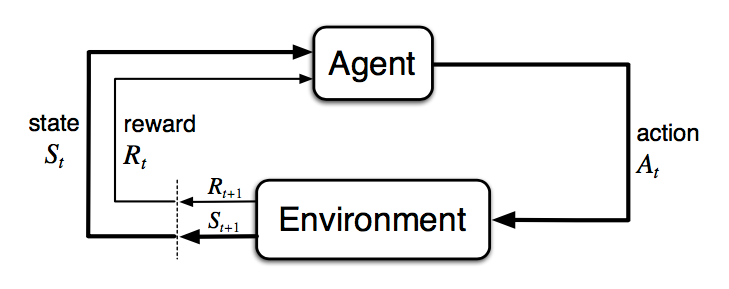
\includegraphics[width=0.6\textwidth]{mdp}
    \caption{Μία τυπική Διαδικασία Απόφασης κατά Markov}
    \label{fig:mdp}
\end{figure}

Όπως είναι προφανές, σκοπός μίας MDP είναι να μεταβούμε σε μία επιθυμητή τελική κατάσταση αρχίζοντας από μία δεδομένη, γνωστή κατάσταση. Εφόσον οι μεταβάσεις μεταξύ των καταστάσεων γίνεται μέσω των διαθέσιμων δράσεων σημαίνει ότι, ιδανικά, θα πρέπει να προσδιορίσουμε μία συνάρτηση:
\begin{align*}
\mathcal{\mu} : \mathcal{S} \rightarrow \mathcal{A}
\end{align*}

Η συνάρτηση $\mathcal{\mu}$ ονομάζεται \textit{πολιτική ή στρατηγική} (policy) και θα είναι στην ουσία ο οδηγός του πράκτορα δια μέσου της MDP, δηλαδή θα είναι ένας κανόνας επιλογής δράσης σε μία δεδομένη κατάσταση. Μπορούμε ίσως να κατανοήσουμε καλύτερα την έννοια της συνάρτησης πολιτικής κάνοντας έναν μικρό παραλληλισμό με το σκάκι. Στις περισσότερες περιπτώσεις τα άτομα που μαθαίνουν σκάκι σε μεγάλο βαθμό και εις βάθος, έρχονται σε επαφή με μεγάλη ποικιλία εκπαιδευτικού υλικού, στο οποίο περιέχονται οι λεγόμενες \textit{βαριάντες}. Μία βαριάντα είναι ένα σύνολο από κινήσεις οι οποίες έχουν αποδειχθεί πολύ χρήσιμες σε κάποιο από τα στάδια του παιχνιδιού. Για παράδειγμα όσον αφορά την αρχή ενός παιχνιδιού, το λεγόμενο \textit{άνοιγμα}, πολύ γνωστές είναι οι βαριάντες "Γαλλική Άμυνα" και η "Βαριάντα Τσιγκορίν". Είναι σύνολα από συγκεκριμένες κινήσεις (ή δράσεις) που οδηγούν σε μία στρατηγικά συμφέρουσα κατάσταση ανοίγματος. Αυτός ακριβώς είναι και ο ρόλος της συνάρτησης πολιτικής ή στρατηγικής στα πλαίσια της ενισχυτικής μάθησης, να παρέχει στον πράκτορα ένα σύνολο από δράσεις, οι οποίες θα τον οδηγήσουν επιτυχώς προς την επιθυμητή τελική κατάσταση (όπως οι βαριάντες οδηγούν τον παίχτη σκακιού στην νίκη). Θα εξετάσουμε αργότερα με ποια κριτήρια θα πρέπει να προσδιορισθεί η συνάρτηση αυτή. Επίσης κρίνεται σκόπιμο να αναφερθεί ότι οι συναρτήσεις πολιτικής διακρίνονται σε \textit{ντετερμινιστικές}, όπως η παραπάνω, και σε \textit{μη-ντετερμινιστικές} \cite{reinflearning}. Στην δεύτερη περίπτωση οι συναρτήσεις πολιτικής ορίζονται ως:
\begin{align*}
\mathcal{\pi} : \mathcal{S} \times \mathcal{A} \rightarrow [0,1]
\end{align*}

Συνήθως στην βιβλιογραφία οι ντετερμινιστικές πολιτικές συμβολίζονται με $\mu$ ενώ οι μη-ντετερμινιστικές με \pi. Αυτόν τον συμβολισμό θα ακολουθήσουμε και εδώ. Οι ντετερμινιστικές συναρτήσεις πολιτικής καθορίζουν πλήρως ποια δράση είναι η καταλληλότερη για την δεδομένη κατάσταση, ενώ οι μη-ντετερμινιστικές συναρτήσεις πολιτικής έχουν στοχαστική λειτουργία και μας δίνουν την πιθανότητα να επιλεγεί μία δράση $\alpha$ όταν ο πράκτορας βρίσκεται σε μία κατάσταση $s$.\\

Τώρα που έχουμε έναν στόχο, δηλαδή τον προσδιορισμό της συνάρτησης $\mathcal{\pi}$ (ή $\mu$), θα πρέπει να σκεφτούμε με τι κριτήρια θα την επιλέξουμε. Για τον σκοπό αυτό χρειαζόμαστε τους εξής ορισμούς \cite{valuefun}:\\

\textbf{Ορισμός} : Το \textit{Αναμενόμενο Κέρδος} (Expected Return) μίας MDP ορίζεται ως:
\begin{align*} 
\displaystyle G_t = \sum_{k=0}^{+\infty} \gamma^k R_{t+k+1}
\end{align*}
όπου $R_t = R(s_t, \alpha, s_{t+1})$. Είναι δηλαδή η τιμή του \textit{προεξοφλημένου} κέρδους (discounted reward) που λαμβάνει ο πράκτορας ξεκινώντας από μία κατάσταση $s_t$ και ακολουθώντας μία συγκεκριμένη δράση. \\

Ο παράγοντας $\gamma$ παίζει διπλό ρόλο. Καταρχάς, το γεγονός ότι είναι μία σταθερή τιμή μικρότερη της μονάδας επιτρέπει στο παραπάνω άπειρο άθροισμα να συγκλίνει ευκολότερα, εφόσον στις περισσότερες περιπτώσεις η συνάρτηση αμοιβής είναι και αυτή μια φραγμένη συνάρτηση. Η φυσική του σημασία είναι η εξής: Καθώς $\gamma \rightarrow 0$ (και κάνοντας τη σύμβαση ότι $0^0 = 1$) παρατηρούμε ότι όλοι οι όροι του αθροίσματος πέραν του $R_{t+1}$ μηδενίζονται. Αυτό σημαίνει ότι ο πράκτορας δρα "μυωπικά", δηλαδή σκοπός του είναι να βρει τρόπο να πάρει το μέγιστο δυνατό κέρδος στο επόμενό του βήμα, χωρίς να έχει μακροπρόθεσμες βλέψεις. Εν αντιθέσει, καθώς $\gamma \rightarrow 1$ ο πράκτορας δίνει όλο και περισσότερο βάρος σε μελλοντικές αμοιβές και δρά έτσι ώστε να έχει μακρυπρόθεσμα το μέγιστο κέρδος.\\

Τέλος δεν είναι δύσκολο να δείξει κανείς ότι:
\begin{align*}
G_t = R_{t+1} + \gamma G_{t+1}
\end{align*}

\textbf{Ορισμός}: (\textit{Συναρτήσεις Αναμενόμενου Κέρδους $V^\pi$ και $Q^\pi$}). Η συνάρτηση $V^\pi$ (V-value function) ορίζεται ως εξής:
\begin{gather*}
V^\pi : \mathcal{S} \rightarrow \mathbb{R}\\
V^\pi (s) = \mathbb{E}\left[G_t | s_t = s, \mathcal{\pi} \right]
\end{gather*}

Η παραπάνω συνάρτηση μας δίνει την αναμενόμενη τιμή του κέρδους του πράκτορα αν, ξεκινώντας από μία κατάσταση $s_t$, ακολουθήσουμε την συνάρτηση πολιτικής $\mathcal{\pi}$. Πρόκεται για μία πραγματική συνάρτηση, δηλαδή για σε κάθε πιθανή κατάσταση αντιστοιχίζει έναν πραγματικό αριθμό. Πέρα από την συνάρτηση $V^\pi$, εξαιρετικής σημασίας και ευρείας εφαρμογής είναι η συνάρτηση $Q^\pi$ (Q-value function) και ορίζεται ως εξής:
\begin{gather*}
Q^\pi : \mathcal{S} \times \mathcal{A} \rightarrow \mathbb{R}\\
Q^\pi (s, \alpha) = \mathbb{E}\left[G_t | s_t = s, \alpha_t = \alpha, \mathcal{\pi} \right]
\end{gather*}

Η συνάρτηση $Q^\pi$ υπολογίζει το αναμενόμενο κέρδος του πράκτορα αν, ξεκινώντας από μία κατάσταση $s_t$, και εκτελώντας μία δράση $\alpha_t$ ακολουθήσουμε την συνάρτηση πολιτικής $\mathcal{\pi}$. Στην πραγματικότητα η συνάρτηση αυτή είναι ένας \textit{πίνακας} διαστάσεων $(dim(\mathcal{S}), dim(\mathcal{A}))$, έχει δηλαδή αριθμό γραμμών ίσο με την διάσταση του χώρου των καταστάσεων και αριθμό στηλών ίσο με την διάσταση του χώρου των δράσεων. Σε όλους τους παραπάνω ορισμούς υποθέσαμε ότι η προς προσδιορισμό συνάρτηση πολιτικής είναι μη-ντετερμινιστική, κάτι που στην πραγματικότητα δεν είναι απαραίτητο να ισχύει. Στην περίπτωση που ψάχνουμε για μία ντετερμινιστική συνάρτηση πολιτικής τότε οι δείκτες και οι εκθέτες $\pi$ αντικαθίστανται από $\mu$.\\

Ο σκοπός του πράκτορα είναι στο τέλος της MDP που ακολουθεί να έχει μαζέψει το μέγιστο δυνατό κέρδος. Για να το κάνει αυτό θα πρέπει να επιλέγει κάθε φορά την εκάστοτε δράση που θα επιφέρει το μεγαλύτερο κέρδος μετάβασης από μία κατάσταση σε μία άλλη. Πρέπει δηλαδή να "μάθει" την συνάρτηση πολιτικής που μεγιστοποιεί το αναμενόμενο κέρδος. Σε μαθηματικούς όρους, συμβολίζουμε με $Q^*(s,\alpha)$ την \textit{βέλτιστη $Q$-συνάρτηση κέρδους} (optimal Q-value function):
\begin{align*}
Q^*(s,\alpha) = \max_{\mathcal{\pi}} Q^\pi(s,\alpha)
\end{align*}
και με $V^{*}(s)$ την \textit{βέλτιστη $V$-συνάρτηση κέρδους} (optimal V-value function):
\begin{align*}
V^{*}(s) =  \max_{\mathcal{\pi}} V^{\pi}(s)
\end{align*}
Για ένα ζεύγος κατάστασης-δράσης $(s, \alpha)$ η συνάρτηση $Q^{*}(s, \alpha)$ δίνει το αναμενόμενο κέρδος όταν, όντας στην κατάσταση $s$ λαμβάνουμε την δράση $\alpha$ και έπειτα ακολουθούμε μία βέλτιστη στρατηγική. Με βάση την σκέψη αυτή μπορούμε να εκφράσουμε την συνάρτηση $Q^{*}$ συναρτήσει της $V^{*}$ ως εξής:
\begin{equation}
Q^{*}(s, \alpha) = \mathbb{E} \left[R_{t+1} + \gamma V^{*}(s_{t+1}) | s_{t} = s, \alpha_{t} = \alpha \right]
\end{equation}

Στόχος μας είναι να προσδιορίσουμε την \textit{βέλτιστη συνάρτηση πολιτικής}, $\pi ^* (s)$, η οποία προφανώς θα ικανοποιεί:
\begin{equation}
\pi^* (s) = \operatorname*{argmin}_{\alpha \in \mathcal{A}} Q^* (s,\alpha)
\end{equation}


Οι παραπάνω συναρτήσεις $Q^\pi$ και $\pi^*$ είναι πρακτικά αδύνατον να υπολογισθούν αναλυτικά, λόγω της μεγάλης πολυπλοκότητάς τους. Συνεπώς θα πρέπει να βρεθεί ένας τρόπος να γίνει μία προσέγγιση αυτών. Όπως θα δούμε παρακάτω, τον ρόλο αυτόν του συναρτησιακού προσεγγιστή θα τον παίξει ένα κατάλληλα σχεδιασμένο νευρωνικό δίκτυο. Θα δημιουργήσουμε δηλαδή δύο ξεχωριστά νευρωνικά δίκτυα, ένα που θα μας υπολογίζει την συνάρτηση $Q^*$ και ένα που θα μας υπολογίζει την συνάρτηση $\pi^*$.\\

\subsection{Εξισώσεις Βελτιστοποίησης Bellman}

Οι εξισώσεις βελτιστοποίησης του Bellman (Bellman Optimality Equations) \cite{sutton} είναι αναδρομικές εξισώσεις που μας δίνουν έναν τρόπο υπολογισμού των βέλτιστων συναρτήσεων κέρδους, $Q^*(s,\alpha)$ και $V^*(s)$ και φαίνονται παρακάτω:  \\

\begin{subequations}
\begin{empheq}[box=\widefbox]{align}
\displaystyle V^*(s) = \max_{\alpha \in \mathcal{A}} \sum_{s' \in \mathcal{S}} \mathcal{P} (s, \alpha, s') \left(\mathcal{R}(s, \alpha, s') + \gamma V^*(s')\right)\\
\displaystyle Q^*(s, \alpha) = \sum_{s' \in \mathcal{S}} \mathcal{P} (s, \alpha, s') \left(\mathcal{R}(s, \alpha, s') + \gamma \max_{\alpha ' \in \mathcal{A}} Q^* (s', \alpha ')\right)
\end{empheq}
\end{subequations}

Οι παραπάνω εξισώσεις στηρίζονται στο γεγονός ότι η τιμή μίας κατάστασης υπό την βέλτιστη στρατηγική, $V^{*}(s)$, θα πρέπει να ισούται με το αναμενόμενο κέρδος για την καλύτερη δράση από αυτήν την κατάσταση, δηλαδή:\\
\begin{align*}
V^{*}(s) = \max_{\alpha \in \mathcal{A}(s)} Q^{\pi^{*}}(s,\alpha)
\end{align*}
Μία σύντομη απόδειξη των αναδρομικών εξισώσεων Bellman παρατίθεται στο παράρτημα.\\

Ένα ενδιαφέρον ερώτημα είναι κατά πόσο οι παραπάνω εξισώσεις μπορούν όντως να δώσουν λύση, δηλαδή αν πράγματι υπάρχει μία βέλτιστη λύση. Θα ασχοληθούμε μόνο με την περίπτωση της συνάρτησης $Q^*(s, \alpha)$ όμως παρόμοιες συλλογιστικές πορείες ισχύουν φυσικά και για την $V^*(s)$. Για να απαντήσουμε στο ερώτημα αυτό θεωρούμε τον \textit{συναρτησιακό τελεστή Bellman} $\mathcal{B}$ \cite{valuefun}, ο οποίος ορίζεται ως εξής: Αν $K: \mathcal{S} \times \mathcal{A} \rightarrow \mathbb{R}$ τότε:
\begin{equation}
\displaystyle (\mathcal{B} K)(s, \alpha) = \sum_{s' \in \mathcal{S}} \mathcal{P}(s, \alpha, s') \left(\mathcal{R}(s, \alpha, s') + \gamma \max_{\alpha ' \in \mathcal{A}} K(s', \alpha ') \right)
\end{equation} 
Η παραπάνω εξίσωση είναι ακριβώς η εξίσωση βελτιστοποίησης του Bellman για μία συνάρτηση $K$. Συνεπώς για να αποδείξουμε την ύπαρξη της βέλτισης λύσης, $Q^*(s,\alpha)$, αρκεί να δείξουμε ότι ο τελεστής Bellman είναι μία \textit{συστολή} (contraction), δηλαδή ικανοποιεί την εξής συνθήκη: Για δύο συναρτήσεις $K_1,K_2 : \mathcal{S} \times \mathcal{A} \rightarrow \mathbb{R}$ ισχύει η ανισότητα:
\begin{align}
||\mathcal{B}(K_1) - \mathcal{B}(K_2)||_{\infty} < ||K_1 - K_2||_{\infty}
\end{align}
Αν καταφέρουμε να δείξουμε ότι ο τελεστής $\mathcal{B}$ είναι συστολή τότε από το \textit{Θεώρημα Σταθερού Σημείου του Banach} θα υπάρχει σταθερό σημείο του τελεστή αυτού και άρα θα υπάρχει μία συνάρτηση που θα ικανοποιεί την εξίσωση βελτιστοποίησης Bellman (η πλήρης διατύπωση του θεωρήματος αυτού καθώς και η απόδειξή του παρατίθενται στο παράρτημα). Σημειώνεται ότι ο λόγος που επιλέγεται η $l ^ {\infty}$ νόρμα στον παραπάνω ορισμό είναι για λόγους ευκολίας πράξεων. Αφού οι χώροι $\mathcal{S}$ και $\mathcal{A}$ είναι πεπερασμένης διάστασης όλες οι νόρμες είναι ισοδύναμες. Έχουμε λοιπόν ότι:\\

$\displaystyle ||\mathcal{B}(K_1) - \mathcal{B}(K_2)||_{\infty}$ =\\ 

$\displaystyle \max_{s, \alpha}  \abs{ \sum_{s' \in \mathcal{S}} \mathcal{P}(s, \alpha, s') (\mathcal{R}(s, \alpha, s') + \gamma \max_{\alpha ' \in \mathcal{A}} K_1 (s', \alpha ') \\
\displaystyle -\sum_{s' \in \mathcal{S}} \mathcal{P}(s, \alpha, s') (\mathcal{R}(s, \alpha, s') + \gamma \max_{\alpha ' \in \mathcal{A}} K_2 (s', \alpha '))} $\\

$\displaystyle= \max_{s, \alpha} \abs{ \sum_{s' \in \mathcal{S}} \mathcal{P} \gamma (\max_{\alpha ' \in \mathcal{A}} K_1 (s', \alpha ') -\max_{\alpha ' \in \mathcal{A}} K_2 (s', \alpha ')) }$\\

$\displaystyle \leq \gamma \max_{s, \alpha}  \sum_{s' \in \mathcal{S}} \abs{ \mathcal{P}} \abs{\max_{\alpha ' \in \mathcal{A}} K_1 (s', \alpha ') -\max_{\alpha ' \in \mathcal{A}} K_2 (s', \alpha ')} \leq \gamma  \max_{s, \alpha}  \sum_{s' \in \mathcal{S}}\abs{\max_{\alpha ' \in \mathcal{A}} K_1 (s', \alpha ') -\max_{\alpha ' \in \mathcal{A}} K_2 (s', \alpha ')}  $\\

Στην τελευταία ανίσωση χρησιμοποιήθηκε το γεγονός ότι η συνάρτηση $\mathcal{P}$ είναι συνάρτηση πιθανότητας και άρα θα ισχύει ότι $\abs{\mathcal{P}} \leq 1$. Συνεχίζουμε παρατηρώντας ότι η ποσότητα μέσα στην απόλυτη τιμή δεν εξαρτάται πλέον από τα $s$ και $\alpha$ :\\

$\displaystyle \gamma  \max_{s, \alpha}  \sum_{s' \in \mathcal{S}}\abs{\max_{\alpha ' \in \mathcal{A}} K_1 (s', \alpha ') -\max_{\alpha ' \in \mathcal{A}} K_2 (s', \alpha ')} = \gamma \sum_{s' \in \mathcal{S}}\abs{\max_{\alpha ' \in \mathcal{A}} K_1 (s', \alpha ') -\max_{\alpha ' \in \mathcal{A}} K_2 (s', \alpha ')} \leq \gamma \max_{s' \in \mathcal{S}} \abs{\max_{\alpha ' \in \mathcal{A}} K_1 (s', \alpha ') -\max_{\alpha ' \in \mathcal{A}} K_2 (s', \alpha ')} = \gamma \max_{s' \in \mathcal{S}, \alpha ' \in \mathcal{A}} \abs{K_1 - K_2} = \gamma ||K_1 - K_2||_{\infty}$\\

Τέλος επειδή $0 \leq \gamma < 1$ παίρνουμε την επιθυμητή ανισότητα. Συνεπώς ο τελεστής Bellman έχει σταθερό σημείο και το πρόβλημα υπάρξης της βέλτιστης λύσης $Q^*(s,\alpha)$ λύθηκε. \\



\subsection{On-Policy και Off-Policy Ενισχυτική Μάθηση}

 Στο σημείο αυτό θα πρέπει να κάνουμε μία μικρή διάκριση στο τί σημαίνει η εκπαίδευση (μέσω ενισχυτικής μάθησης) να είναι on-policy και off-policy. Με απλά λόγια ένας πράκτορας που εκπαιδεύεται με on-policy ενισχυτική μάθηση μαθαίνει για το περιβάλλον ακολουθώντας μία πολιτική $\pi$ και ταυτόχρονα οι παρατηρήσεις του και οι εμπειρίες του στο περιβάλλον αυτό παράγονται με βάση την ίδια αυτή πολιτική $\pi$. Ο πράκτορας δηλαδή μαθαίνει πόσο καλό είναι να κάνει κάτι κάνοντάς το. Εν αντιθέσει, ένας πράκτορας που εκπαιδεύεται με off-policy ενισχυτική μάθηση μαθαίνει το περιβάλλον με την χρήση μίας πολιτικής $\pi_{1}$ αλλά οι εμπειρίες και το κέρδος του πράκτορα παράγονται από μία άλλη πολιτική $\pi_{2}$. Ο πράκτορας δηλαδή μαθαίνει πόσο καλό είναι να κάνει κάτι κάνοντας κάτι άλλο. Η λεγόμενη \textit{Q-εκμάθηση} είναι ένα παράδειγμα off-policy αλγορίθμου \cite{sutton}:\\

\begin{table}[H]
\begin{tabular}{ |p{13cm}}
 \hline
 \multicolumn{1}{|c|}{\textbf{Αλγόριθμος Q-εκμάθησης}} \\
 \hline
 Καθορισμός παραμέτρων αλγορίθμου: βήμα εκπαίδευσης $\tau \in (0,1]$, $\gamma \in (0,1]$ και ένα μικρό $\epsilon > 0$ \\
 Αρχικοποίηση πίνακα $Q(s,\alpha)$ για κάθε $s \in \mathcal{S}$, $\alpha \in \mathcal{A}$, αυθαίρετα εκτός από $Q(final, \cdot) = 0$  \\
 \textbf{For} each episode \textbf{do}:\\
Αρχικοποίηση μίας κατάστασης $s$ \\
\textbf{For} each time step of episode \textbf{do}:  \\
Επιλογή μιας $A \in \mathcal{A}$ από την $s$ μέσω μίας πολιτικής που παράγεται από την Q, έστω $\pi_{1}$\\
Λήψη της δράσης $A$, παρατήρηση των $s'$ και $R$\\
$Q(s, A) \leftarrow Q(s, A) + \tau[R + \gamma \max_{\alpha}Q(s', \alpha) - Q(s, A)]$\\
$s \leftarrow s'$\\
μέχρι την τερματική κατάσταση $s_{T}$\\
\hline
\end{tabular}
\caption{Off-policy Αλγόριθμος Q-εκμάθησης}
\end{table}

Παρατηρούμε ότι στον αλγόριθμο Q-εκμάθησης ο πράκτορας μαθαίνει την βέλτιστη στρατηγική (στρατηγική ή πολιτική επικαιροποίησης, update policy) χρησιμοποιώντας την πολιτική $\pi(s) = \max_{\alpha}Q(s', \alpha)$, η οποία στην βιβλιογραφία αναφέρεται και ως \textit{άπληστη στρατηγική} (greedy policy), όμως συμπεριφέρεται και δρά (επιλέγει δηλαδή την επόμενη κατάσταση) σύμφωνα με την πολιτική $\pi_{1}$ (στρατηγική ή πολιτική συμπεριφοράς, behaviour policy). Ακριβώς επειδή η πολιτική επικαιροποίησης και η πολιτική συμπεριφοράς είναι διαφορετικές ο αλγόριθμος χαρακτηρίζεται ως off-policy. Όταν οι δύο πολιτικές αυτές είναι ίδιες τότε ο αλγόριθμος χαρακτηρίζεται ως on-policy. Ένας τέτοιος αλγόριθμος είναι και ο αλγόριθμος SARSA \cite{sutton}:\\

\begin{table}[H]
\begin{tabular}{ |p{13cm}}
 \hline
 \multicolumn{1}{|c|}{\textbf{Αλγόριθμος SARSA}} \\
 \hline
 Καθορισμός παραμέτρων αλγορίθμου: βήμα εκπαίδευσης $\tau \in (0,1]$, $\gamma \in (0,1]$ και ένα μικρό $\epsilon > 0$ \\
 Αρχικοποίηση πίνακα $Q(s,\alpha)$ για κάθε $s \in \mathcal{S}$, $\alpha \in \mathcal{A}$, αυθαίρετα εκτός από $Q(final, \cdot) = 0$  \\
 \textbf{For} each episode \textbf{do}:\\
Αρχικοποίηση μίας κατάστασης $s$ \\
\textbf{For} each time step of episode \textbf{do}:  \\
Επιλογή μιας $A \in \mathcal{A}$ από την $s$ μέσω μίας πολιτικής που παράγεται από την Q, έστω $\pi_{1}$\\
Λήψη της δράσης $A$, παρατήρηση των $s'$ και $R$\\
Επιλογή μιας $Α' \in \mathcal{A}$ από την $s'$ μέσω της ίδιας πολιτικής $\pi_{1}$\\
$Q(s, A) \leftarrow Q(s, A) + \tau[R + \gamma Q(s', A') - Q(s, A)]$\\
$s \leftarrow s'$ και $Α \leftarrow A'$\\
μέχρι την τερματική κατάσταση $s_{T}$\\
\hline
\end{tabular}
\caption{On-policy Αλγόριθμος SARSA}
\end{table}

Βλέπουμε λοιπόν ότι η ενισχυτική μάθηση είναι στην ουσία ένα "παιχνίδι", στο οποίο ο παίχτης προσπαθεί να φτάσει σε μία τελική κατάσταση (ουσιαστικά στην νίκη του παιχνιδιού) μαζεύοντας κατά το δυνατόν περισσότερο κέρδος. Φυσικά για έναν άνθρωπο, που μαθαίνει με βιολογικό τρόπο, αυτό το κέρδος δεν έχει κάποιο ιδιαίτερο φυσικό νόημα. Το συσσωρευμένο κέρδος είναι ο τρόπος με τον οποίο βοηθάμε τον υπολογιστή μας να καταλάβει κατά πόσο βρίσκεται στην σωστή πορεία μέσα σε αυτό το παιχνίδι (όπως βοηθάμε το ζώο να καταλάβει κατά πόσο είμαστε ικανοποιημένοι με την συμπεριφορά του δίνοντας του κάτι να φάει). Η ενισχυτική μάθηση βρίσκεται στο ζενίθ της σύγχρονης τεχνητής νοημοσύνης καθώς βρίσκει εφαρμογή σε ποικίλες εφαρμογές, όπως για παράδειγμα στην οδήγηση οχημάτων, στη ρομποτική καθώς και σε πολλά πραγματικά παιχνίδια \cite{atari}.  \\

\newpage

\section{Ενισχυτική Μάθηση Βάθους (Deep Reinforcement Learning)}

\subsection{Εισαγωγή και Ιστορική Αναδρομή}

Έχοντας τώρα την θεωρία της εκπαίδευσης των νευρωνικών δικτύων και της ενισχυτικής μάθησης μπορούμε να τις συνδυάσουμε με έναν φυσικό τρόπο για να δημιουργήσουμε την θεωρία της \textit{Ενισχυτικής Μάθησης Βάθους}. Όπως έχει ήδη προαναφερθεί, τα νευρωνικά δίκτυα στην ουσία δρουν ως συναρτησιακοί προσεγγιστές, δηλαδή εκφράζουν μία συνάρτηση ως έναν γραμμικό συνδιασμό σιγμοειδών συναρτήσεων. Επίσης θυμόμαστε από την θεωρία της ενισχυτικής μάθησης ότι ο στόχος μας είναι να προσιορίσουμε τις συναρτήσεις $\mu^{*}(s)$ και $Q^{*}(s, \alpha)$. Η θεωρία της ενισχυτικής μάθησης βάθους συνδυάζει ακριβώς αυτά τα δύο πράγματα. Προσπαθούμε να προσδιορίσουμε τις συναρτήσεις $\mu^{*}(s)$ και $Q^{*}(s, \alpha)$ με νευρωνικά δίκτυα. Ένα νευρωνικό δίκτυο θα προσδιορίζει την συνάρτηση $\mu^{*}(s)$ και θα λέγεται \textit{δράστης} και ένα άλλο νευρωνικό δίκτυο θα προσδιορίζει την συνάρτηση  $Q^{*}(s, \alpha)$ και θα λέγεται \textit{κριτής}. Η οντότητα που αποτελείται από έναν δράστη και έναν κριτή θα λέγεται \textit{πράκτορας} (agent) και θα αποτελεί στην ουσία τον ρυθμιστή της διεργασίας μας. Πρίν όμως συνεχίσουμε με την μαθηματική θεμελίωση της ενισχυτικής μάθησης βάθους θα κάνουμε μία σύντομη ιστορική αναδρομή που σχετίζεται με την εκπληκτική επίδοση της εφαρμογής της εν λόγω θεωρίας.  \\

Θα είναι λογικό να αναμένει κανείς πως ηλεκτρονικά παιχνίδια, όπως αυτά που έχουν φτιαχτεί για την κονσόλα Atari, αλλά και επιτραπέζια παιχνίδια όπως το σκάκι, θα αποτελούν επιλογή και προνόμιο μόνο ενός ανθρώπου, δηλαδή ενός όντος με \textit{συνείδηση}. Το σκεπτικό αυτό καταρρίφθηκε ήδη από τον Μάιο του 1997, όπου το υπερυπολογιστικό σύστημα Deep Blue της IBM κατάφερε να νικήσει τον παγκόσμιο πρωταθλητή σκακιού, Garry Kasparov. Ο τρόπος με τον οποίο κατάφερε ο υπολογιστής αυτός αυτό το επίτευγμα είναι αξιοποιώντας έναν τεράστιο όγκο δεδομένων από παρτίδες σκακιού, έτσι ώστε να "μάθει" το παιχνίδι και στην συνέχεια, με την βοήθεια ορισμένων αλγορίθμων βελτιστοποίησης (που ανήκουν στον κλάδο της μηχανικής μάθησης), μπόρεσε να "καταλάβει" ποιες κινήσεις και στρατηγικές είναι οι καταλληλότερες για να κερδίσει. Αυτό και μόνο είναι εντυπωσιακό. Ένα ακόμη πιο εντυπωσιακό επίτευγμα ήρθε από την Deep Mind το 2013.\\

Οι άνθρωποι της Deep Mind κατάφεραν να φτιάξουν ένα σύστημα τεχνητής νοημοσύνης το οποίο μπορούσε να παίξει (μεταξύ άλλων) το ηλεκτρονικό παιχνίδι \textit{Breakout}. Αυτό στην αρχή μπορεί να φαίνεται σαν ένα τίποτα μπροστά στην νίκη του Deep Blue αφού το παιχνίδι \textit{Breakout} είναι, όπως μπορεί κάποιος να επιβεβαιώσει άμεσα παιζοντάς το στο διαδίκτυο, πολύ απλό και εύκολο σε σχέση με το σκάκι. Δεν απαιτεί ούτε ιδιαίτερη νοημοσύνη ούτε πολλές ικανότητες. Όμως η μέθοδος της Deep Mind δεν έπαιξε απλά το παιχνίδι. Στην πραγματικότητα είχαν δημιουργήσει ένα σύστημα τεχνητής νοημοσύνης που δεν γνώριζε \textit{απολύτως τίποτα} για το παιχνίδι, ούτε καν για \textit{έννοιες} όπως παιχνίδι, ρακέτες, τούβλα ή τοίχος \cite{max} (στοιχεία που υπάρχουν στο \textit{Breakout}). Το μόνο "δεδομένο" που διέθετε το σύστημα τεχνητής νοημοσύνης ήταν η βαθμολογία (score) του παιχνιδιού, την οποία είχε ως στόχο να μεγιστοποιήσει. Έπρεπε δηλαδή να μάθει από την αρχή το παιχνίδι χωρίς οδηγίες, απλά παίζοντάς το. Οι αρχικές του επιδόσεις ήταν άθλιες. Καθώς περνούσε όμως ο χρόνος τα κατάφερνε όλο και καλύτερα μέχρι ωσότου να γίνει κάτι "μαγικό". Το σύστημα αυτό κατάφερε να βρει έναν πανέξυπνο τρόπο για να μεγιστοποιήσει την βαθμολογία του και ο τρόπος αυτός αναδεικνύεται καλύτερα στο βίντεο που βρίσκεται στο τέλος των ηλεκτρονικών παραπομπών. Η μέθοδος που χρησιμοποίησαν δεν ήταν άλλη από την ενισχυτική μάθηση βάθους. Η ίδια μέθοδος έχει διαπρέψει και σε πολλά άλλα ηλεκτρονικά παιχνίδια \cite{atari}. Όμως ακόμη και αυτό δεν είναι τίποτα μπροστά στο επόμενο επίτευγμα.\\

Το επόμενο σύστημα τεχνητής νοημοσύνης της Deep Mind, με όνομα \textit{AlphaGo}, κατάφερε να εκθρονίσει τον παγκόσμιο πρωταθλητή του παιχνιδιού \textit{Go}, Lee Sedol, τον Μάρτιο του 2016 \cite{max}. Το παιχνίδι \textit{Go} είναι ένα παιχνίδι στρατηγικής, όπως το σκάκι, που όμως έχει απίστευτα μεγαλύτερη πολυπλοκότητα. Σε τάξεις μεγέθους, το σκάκι (το οποίο αποτελείται από μία σκακιέρα $8 \times 8$ και έχει συνολικά 32 πιόνια και για τους δύο παίχτες) περιλαμβάνει \textit{μόνο} περίπου $10 ^ {43}$ πιθανούς συνδυασμούς στους οποίους μπορούν να τοποθετηθούν τα πιόνια ακολουθώντας τους κανόνες του παιχνιδιού. Το \textit{Go} (το οποίο παίζεται σε μία σκακιέρα $19 \times 19$) περιλαμβάνει περίπου \textit{$10 ^ {172}$} πιθανούς συνδυασμούς! Για να καταλάβουμε πόσο ασύλληπτα μεγάλος είναι αυτός ο αριθμός, έχει υπολογισθεί ότι ο αριθμός των ατόμων στο παρατηρήσιμο σύμπαν είναι της τάξεως των $10 ^{80}$! Πριν τον κρίσιμο αγώνα, όλοι πίστευαν πως μόνο ένας οργανισμός όπως ο άνθρωπος θα μπορέσει ποτέ να παίξει ένα τόσο σύνθετο παιχνίδι. Όταν όμως ο \textit{AlphaGo} νίκησε \textit{τρεις φορές} τον Lee Sedon τα πράγματα άλλαξαν ριζικά. Οι ικανότητες που είχε προσφέρει η ενισχυτική μάθηση βάθους στην επιστήμη της τεχνητής νοημοσύνης ήταν αδιαμφισβήτητες. Ένας υπολογιστής μπόρεσε στην κυριολεξία να \textit{μάθει} ένα τόσο περίπλοκο παιχνίδι, χωρίς να ξέρει απολύτως τίποτα για αυτό απλά παίζοντάς το πολλές φορές. \\

Κλείνουμε τώρα αυτό το μικρό αλλά πολύ ενδιαφέρον παράθυρο στην ιστορία της τεχνητής νοημοσύνης και συνεχίζουμε με την περιγραφή των μαθηματικών συνιστωσών που συναποτελούν την θεωρία της ενισχυτικής μάθησης βάθους. Καταρχάς ας θυμηθούμε ότι στόχος μας είναι να εκπαιδεύσουμε δύο νευρωνικά δίκτυα που θα προσεγγίζουν τις συναρτήσεις $\mu^{*}(s)$ και $Q^{*}(s, \alpha)$ καθώς και ότι με "εκπαίδευση" νευρωνικών δικτύων εννοούμε τον προσδιορισμό των βέλτιστων βαρών και biases. Θα πρέπει λοιπόν τώρα, αν θέλουμε να προσδιορίσουμε τις παραπάνω συναρτήσεις, να καταφέρουμε να τις κάνουμε συναρτήσεις και των παραμέτρων του αντίστοιχου δικτύου που θα τις παράγει.

\subsection{Αλγόριθμοι Ντετερμινιστικής Βαθμίδας Πολιτικής (Deterministic Policy Gradient Algorithms)}
Οι αλγόριθμοι ντετερμινιστικής βαθμίδας πολιτικής χρησιμοποιούνται κατα κόρον σε προβλήματα ενισχυτικής μάθησης με συνεχή χώρο δράσεων \cite{dpga}. Η βαθμίδα της ντετερμινιστικής πολιτικής είναι η αναμενόμενη τιμή της βαθμίδας της συνάρτησης που παίρνει ως τιμές τις δράσεις. Η βασική δηλαδή ιδέα είναι να αναπαραστίσουμε την ντετερμινιστική συνάρτηση πολιτικής, $\mu_{\theta} : \mathcal{S} \rightarrow \mathcal{A}$, με μία παραμετρική κατανομή πιθανότητας $\pi_{\theta}(\alpha | s) = \mathbb{P}[\alpha | s;\theta]$, η οποία στοχαστικά επιλέγει μία δράση $\alpha$ σε μια κατάσταση s βασιζόμενη στο διάνυσμα των παραμέτρων $\theta$. Οι αλγόριθμοι βαθμίδας πολιτικής παίρνουν δείγματα μέσα από αυτήν την κατανομή και προσαρμόζουν το διάνυσμα των παραμέτρων $\theta$ προς την κατεύθυνση του μεγαλύτερου συσσωρευμένου κέρδους. Για να συνεχίσουμε θα πρέπει να τοποθετηθούμε και πάλι σε μία διαδικασία απόφασης κατά Markov. Υποθέτουμε δηλαδή ότι έχουμε δεδομένο έναν (συνεχή) χώρο καταστάσεων $\mathcal{S}$, έναν (συνεχή) χώρο δράσεων $\mathcal{A}$, μία συνάρτηση μετάβασης $\mathcal{P}$ που ικανοποιεί την Μαρκοβιανή ιδιότητα για κάθε αλυσίδα $s_{1}, \alpha_{1}, s_{2}, \alpha_{2}, \cdots, s_{T}, \alpha_{T}$ στον χώρο των δράσεων, μία συνάρτηση κέρδους $R : \mathcal{S} \times \mathcal{A} \rightarrow \mathbb{R}$ και έναν παράγοντα προεξόφλησης \gamma. $\theta \in \mathbb{R}^{n}$ είναι ένα διάνυσμα $n$ παραμέτρων και $\pi_{\theta}(\alpha_{t}|s_{t})$ είναι η δεσμευμένη πυκνότητα πιθανότητας στην $\alpha_{t}$. Ο πράκτορας χρησιμοποιεί την πολιτική για να αλληλεπιδράσει με το περιβάλλον και δίνει την τροχία $h_{1 \rightarrow T} = s_{1}, \alpha_{1}, R_{1}, s_{2}, \alpha_{2}, R_{2}, \cdots, s_{T}, \alpha_{T}, R_{T}$. Συμβολίζουμε με $\displaystyle R^{\gamma}_{t} = \sum_{k=t}^{\infty} \gamma^{k-t}R(s_{k}, \alpha_{k})$. Οι συναρτήσεις αναμενόμενου κέρδους είναι οι $V^{\mu}(s) = \mathbb{E}[R^{\gamma}_{1}|s_{1} = s;\mu]$ και $Q^{\mu}(s,\alpha) = \mathbb{E}[R^{\gamma}_{1}|s_{1}=s, \alpha_{1}=\alpha;\mu]$. Στόχος του πράκτορα είναι να βρει εκείνη την πολιτική που μεγιστοποιεί το συσσωρευμένο προεξοφλημένο κέρδος, το οποίο συμβολίζουμε με $\mathcal{J}(\mu) = \mathbb{E}[R^{\gamma}_{1}|\mu]$. Επίσης συμβολίζουμε την πυκνότητα πιθανότητας στην κατάσταση $s'$ αφού μεταβούμε για $t$ χρονικά βήματα από την κατάσταση $s$ με $p(s \rightarrow s', t, \pi)$. Τέλος συμβολίζουμε την προεξοφλημένη κατανομή κατάστασης , $\int_{\mathcal{S}} \sum_{t=1}^{\infty} \gamma^{t-1}p_{1}(s)p(s \rightarrow s', t, \mu)ds$, με $\rho^{\mu}(s')$ \cite{dpga2}, όπου $p_{1}(s)$ η πυκνότητα πιθανότητας της αρχικής κατάστασης $s_{1}$. Με όλους τους παραπάνω συμβολισμούς μπορούμε να εκφράσουμε την αντικειμενική συνάρτησης $\mathcal{J}$ ως εξής \cite{dpga}:
\begin{align*}
\mathcal{J}(\mu_{\theta}) = \int_{\mathcal{S}} \rho^{\mu}(s) R(s,\mu_{\theta}(s))ds = \mathbb{E}_{s \sim \rho^{\mu}}[R(s,\mu_{\theta}(s))]
\end{align*}
Τα σύνολα $\mathcal{S}$ και $\mathcal{A}$ θεωρούμε ότι είναι συμπαγή υποσύνολα του ευκλείδιου χώρου. Τώρα είμαστε έτοιμοι να δώσουμε το βασικό θεώρημα των αλγορίθμων ντετερμινιστικής βαθμίδας \cite{dpga}.\\

\textbf{Θεώρημα Βαθμίδας Ντετερμινιστικής Πολιτικής} : Ας υποθέσουμε ότι οι βαθμίδες $\nabla_{\theta}\mu_{\theta}(s)$ και $\nabla_{\alpha}Q^{\mu}(s,\alpha)$ υπάρχουν και είναι συνεχείς συναρτήσεις. Τότε η βαθμίδα της συνάρτησης κόστους ως προς το διάνυσμα των παραμέτρων, $\nabla_{\theta} \mathcal{J}(\mu_{\theta})$, δίνεται από την σχέση:
\begin{equation}
\displaystyle \nabla_{\theta} \mathcal{J}(\mu_{\theta}) = \int_{\mathcal{S}} \rho^{\mu}(s) \nabla_{\theta} \mu_{\theta}(s) \nabla_{\alpha}Q^{\mu}(s, \alpha)|_{\alpha = \mu_{\theta}(s)} ds = \mathbb{E}_{s \sim \rho^{\mu}}[\nabla_{\theta} \mu_{\theta}(s) \nabla_{\alpha} Q^{\mu}(s,\alpha)]
\end{equation}

Στην συνέχεια θα χρησιμοποιήσουμε το παραπάνω θεώρημα για να εξάγουμε τους περίφημους Ντετερμινιστικούς Αλγόριθμους Δράστη-Κριτή. Όπως και στην περίπτωση της απλής ενισχυτικής μάθησης, έτσι και εδώ, οι αλγόριθμοι αυτοί διακρίνονται σε on-policy και off-policy.\\

\subsection{Ντετερμινιστικοί Αλγόριθμοι Δράστη-Κριτή (Deterministic Actor-Critic Algorithms)}

Οι αλγόριθμοι τύπου δράστη-κριτή χρησιμοποιούνται για την βελτιστοποίηση διαδικασιών απόφασης Markov που χαρακτηρίζονται από παραμετρικοποιημένες οικογένειες συναρτήσεων πολιτικής (parametrized policies) \cite{actorcritic}. Είναι δηλαδή αλγόριθμοι στοχαστικής βαθμίδας στον παραμετρικοποιημένο χώρο του δράστη. Στην πραγματικότητα πρόκειται για δύο παράλληλους αλγόριθμους. Στον έναν αλγόριθμο ο κριτής χρησιμοποιεί \textit{Εκμάθηση Χρονικής Διαφοράς} (Temporal Difference Learning ή TD-Learning), μία έννοια που θα παρουσιασθεί αργότερα, με μία αρχιτεκτονική γραμμικής προσέγγισης για να μάθει την συνάρτηση αναμενόμενης τιμής, $Q(s, \alpha)$, και στον άλλο ο δράστης επικαιροποιείται με βάση την κατεύθυνση μίας προσεγγιστικής βαθμίδας βασισμένης σε πληροφορίες που παρέχονται από τον κριτή. \\

\begin{itemize}
\item On-policy Ντετερμινιστικός Αλγόριθμος Δράστη-Κριτή
\end{itemize}
Όπως προαναφέρθηκε, ο αλγόριθμος αυτός έχει δύο συνιστώσες. Ο κριτής υπολογίζει τον πίνακα-συνάρτηση $Q(s, \alpha)$ και ο δράστης χρησιμοποιεί την συνάρτηση αυτή για να υλοποιήσει Gradient Ascent της βαθμίδας της Q. Πιο συγκεκριμένα, ο δράστης προσαρμόζει τις παραμέτρους $\theta$ (οι οποίες άτυπα προς το παρόν μέσα στο μυαλό μας είναι οι παράμετροι των νευρωνικών δικτύων, δηλαδή τα βάρη και τα biases) της ντετερμινιστικής πολιτικής $\mu_{\theta}(s)$ μέσω στοχαστικού Gradient Ascent που περιγράφεται από την εξίσωση (6.2.1.). Η μόνη διαφορά με την εξίσωση αυτή είναι ότι στην θέση της ακριβούς συνάρτησης $Q^{\mu}(s,\alpha)$ μπαίνει μία προσέγγιση αυτής, $Q^{w}(s,\alpha)$ \cite{dpga}. Ο κριτής υπολογίζει προσεγγιστικά την $Q^{w}(s,\alpha) \approx Q^{\mu}(s,\alpha)$ με την χρήση κάποιου αλγορίθμου όπως η SARSA. Τα βήματα ενός τέτοιου αλγορίθμου φαίνονται παρακάτω \cite{sutton}:
\begin{align*}
\delta_{t} = R_{t} + \gamma Q^{w}(s_{t+1},\alpha_{t+1}) - Q^{w}(s_{t},\alpha_{t})\\
w_{t+1} = w_{t} + \tau_{w} \delta_{t} \nabla_{w} Q^{w}(s_{t},\alpha_{t})\\
\theta_{t+1} = \theta_{t} + \tau_{\theta} \nabla_{\theta} \mu_{\theta}(s_{t}) \nabla_{\alpha} Q^{w}(s_{t},\alpha_{t})|_{\alpha = \mu_{\theta}(s)}
\end{align*}

Το διάνυσμα των παραμέτρων $w$ (και όσες παράμετροι φέρουν δείκτη $w$, όπως ο $\tau_{w}$) αναφέρεται στην προσεγγιστική συνάρτηση $Q^{w}(s,\alpha)$. Οι τιμές αυτές χρησιμοποιούνται τέλος για την επικαιροποίηση του διανύσματος των παραμέτρων $\theta$, το οποίο αναφέρεται στην πραγματική επιθυμητή προς προσδιορισμό συνάρτηση $Q^{\mu}(s,\alpha)$. Τέλος σημειώνεται ότι η ποσότητα $\delta_{t}$ ονομάζεται \textit{Χρονική Διαφορά} (Temporal Difference).\\

\begin{itemize}
\item Off-policy Ντετερμινιστικός Αλγόριθμος Δράστη-Κριτή
\end{itemize}
Θα εξετάσουμε τώρα την περίπτωση μίας off-policy μεθόδου που μαθαίνει μία ντετερμινιστική πολιτική $\mu_{\theta}(s)$ (update policy) μέσω μίας αυθαίρετης στοχαστικής πολιτικής $\beta(s,\alpha) \neq \pi_{\theta}(s,\alpha) $ (behaviour policy) \cite{dpga}. Στην περίπτωση αυτή η αντικειμενική συνάρτηση θα έχει την εξής μορφή:
\begin{align*}
\mathcal{J}_{\beta}(\mu_{\theta}) = \int_{\mathcal{S}} \rho^{\beta}(s) Q^{\mu}(s, \mu_{\theta}(s))ds
\end{align*}

Τώρα το Θεώρημα Ντετερμινιστικής Βαθμίδας μας δίνει την εξής προσέγγιση \cite{dpga}:
\begin{equation}
\nabla_{\theta} \mathcal{J}_{\beta}(\mu_{\theta}) \approx \int_{\mathcal{S}} \rho^{\beta}(s) \nabla_{\theta} \mu_{\theta}(\alpha | s) Q^{\mu}(s,\alpha) ds = \mathbb{E}_{s \sim \rho^{\beta}}\left[\nabla_{\theta} \mu_{\theta}(s) \nabla_{\alpha} Q^{\mu}(s,\alpha)|_{\alpha = \mu_{\theta}(s)}\right]
\end{equation}

Η παραπάνω εξίσωση δίνει την off-policy βαθμίδα ντετερμινιστικής πολιτικής. Είμαστε έτοιμοι τώρα να αναπτύξουμε έναν αλγόριθμο δράστη-κριτή που επικαιροποιεί την πολιτική στην κατεύθυνση της off-policy βαθμίδας της ντετερμινιστικής πολιτικής. Ομοίως με προηγουμένως, αντικαθιστούμε την ακριβής λύση $Q^{\mu}(s,\alpha)$ με μία προσέγγιση $Q^{w}(s,\alpha)$. Ο κριτής υπολογίζει την συνάρτηση $Q^{w}(s,\alpha) \approx Q^{\mu}(s,\alpha)$ από τροχιές που παράγονται από την $\beta(s,\alpha)$ χρησιμοποιώντας έναν κατάλληλο αλγόριθμο. Στο παρακάτω αλγόριθμο ο κριτής χρησιμοποιεί Q-εκμάθηση για να υπολογίσει την συνάρτηση $Q^{\mu}$ \cite{sutton}:
\begin{align*}
\delta_{t} = R_{t} + \gamma Q^{w}(s_{t+1},\mu_{\theta}(s_{t+1}) - Q^{w}(s_{t},\alpha_{t})\\
w_{t+1} = w_{t} + \tau_{w} \delta_{t} \nabla_{w} Q^{w}(s_{t},\alpha_{t})\\
\theta_{t+1} = \theta_{t} + \tau_{\theta} \nabla_{\theta} \mu_{\theta}(s_{t}) \nabla_{\alpha} Q^{w}(s_{t},\alpha_{t})|_{\alpha = \mu_{\theta}(s)}
\end{align*}

Στην συνέχεια θα κάνουμε μία μικρή συζήτηση όσον αφορά την προσεγγιστική λύση $Q^{w}(s,\alpha)$. Εν γένει, η αντικατάσταση μίας προσέγγισης $Q^{w}(s,\alpha)$ στην ντετερμινιστική βαθμίδα πολιτικής δεν θα ακολουθήσει απαραίτητα την πραγματική βαθμίδα (και στην πραγματικότητα η πορεία που θα ακολουθήσει μπορεί να μην είναι καν πορεία ανάβασης βαθμίδας). Θα πρέπει δηλαδή η προσέγγιση, $Q^{w}(s,\alpha)$, να πληροί τις απαραίτητες προϋποθέσεις ώστε η βαθμίδα $\nabla_{\alpha}Q^{\mu}(s,\alpha)$ να μπορεί να αντικατασταθεί από την βαθμίδα $\nabla_{\alpha}Q^{w}(s,\alpha)$ χωρίς να επηρεάζεται η βαθμίδα της ντετερμινιστικής πολιτικής.\\ 

Θα λέμε ότι η συναρτησιακή προσέγγιση $Q^{w}(s,\alpha)$ είναι \textit{συμβατή} με την ντετερμινιστική πολιτική \cite{dpga} όταν ισχύει ότι $\nabla_{\theta} \mathcal{J}_{\beta}(\theta) = \mathbb{E}_{s \sim \rho^{\beta}} \left[ \nabla_{\theta} \mu_{\theta}(s) \nabla_{\alpha} Q^{w}(s,\alpha)|_{\alpha = \mu_{\theta}(s)}\right]$, αν πρόκειται για off-policy και $\nabla_{\theta} \mathcal{J}(\theta) = \mathbb{E}_{s \sim \rho^{\mu}} \left[ \nabla_{\theta} \mu_{\theta}(s) \nabla_{\alpha} Q^{w}(s,\alpha)|_{\alpha = \mu_{\theta}(s)}\right]$ αν πρόκειται για on-policy . Τις προϋποθέσεις για να είναι μία συναρτησιακή προσέγγιση συμβατή με μία ντετερμινιστική πολιτική μας τις δίνει το παρακάτω θεώρημα \cite{dpga}:\\

\textbf{Θεώρημα Συμβατότητας Συναρτησιακής Προσέγγισης}: Μία συναρτησιακή προσέγγιση $Q^{w}(s,\alpha)$ είναι συμβατή με μία ντετερμινιστική πολιτική, $\mu_{\theta}(s,\alpha)$ εάν:\\

1) $\nabla_{\alpha} Q^{w}(s,\alpha)|_{\alpha = \mu_{\theta}(s)} = \nabla_{\theta} \mu_{\theta}(s) ^ \intercal w$\\

2) Το διάνυσμα των παραμέτρων w ελαχιστοποιεί το μέσο τετραγωνικό σφάλμα $MSE(\theta, w) = \mathbb{E}\left[\epsilon(s;\theta,w)^\intercal \epsilon(s;\theta, w)\right]$, όπου $\epsilon(s;\theta,w) = \nabla_{\alpha}Q^{w}(s,\alpha)|_{\alpha = \mu_{\theta}(s)} - \nabla_{\alpha}Q^{\mu}(s,\alpha)|_{\alpha = \mu_{\theta}(s)}$\\

Το θεώρημα ισχύει τόσο στην on-policy όσο και στην off-policy περίπτωση. Η απόδειξη είναι απλή και παρατίθεται στο παράρτημα.\\


\subsection{Τα Νευρωνικά Δίκτυα του Δράστη και του Κριτή}
Έχοντας τώρα θεμελιώσει την βασική θεωρία πίσω από τους αλγορίθμους δράστη-κριτή θα πρέπει να βάλουμε στο παιχνίδι και τα νευρωνικά δίκτυα. Ο λόγος που είναι απαραίτητη η εισαγωγή τους είναι επειδή χρειαζόμαστε μία μαθηματική αρχιτεκτονική η οποία θα δράσει ως συναρτησιακός προσεγγιστής τόσο για την ντετερμινιστική συνάρτηση πολιτικής $\mu(s)$ όσο και για την συνάρτηση $Q(s,\alpha)$. Όπως έχει ήδη αναφερθεί στην εισαγωγή αυτού του κεφαλάιου το νευρωνικό δίκτυο που θα υπολογίζει σε κάθε χρονικό βήμα την συνάρτηση πολιτικής θα λέγεται δράστης και το νευρωνικό δίκτυο που θα υπολογίζει την συνάρτηση Q θα λέγεται κριτής. Θα εξετάσουμε τώρα την αρχιτεκτονική του κάθε δικτύου ξεχωριστά.\\

\textbf{Δράστης}: Είσοδος για το νευρωνικό δίκτυο του δράστη (δηλαδή το στρώμα εισόδου) θα αποτελεί η \textit{τρέχουσα κατάσταση} του συστήματος. Η διάσταση του διανύσματος της κατάστασης θα είναι ίση με τον αριθμό των κόμβων ή νευρώνων του στρώματος εισόδου του δικτύου. Στην συνέχεια η πληροφορία αυτή θα \textit{προωθείται} κατά μήκος του δικτύου με βάση την διαδικασία του feed-forward που περιγράφηκε στο κεφάλαιο \textbf{4}. Το διάνυσμα των παραμέτρων του δράστη, δηλαδή τα βάρη και τα biases του θα τα συμβολίσουμε με $\textbf{W}_{α}$. Η πληροφορία φτάνει τελικά στο στρώμα εξόδου του δράστη, η οποία θα δίνει ως αποτέλεσμα την \textit{δράση}, \alpha(t). Η διάσταση του διανύσματος της δράσης θα είναι ίση με τον αριθμό των κόμβων ή νευρώνων του στρώματος εξόδου. Με αυτόν τον τρόπο προκύπτει προφανώς μία συνάρτηση, η δράση, η οποία έχει κληρονομήσει όλες τις παραμέτρους του νευρωνικού δικτύου μέσω της προώθησης. Σχηματίστηκε έτσι δηλαδή μία προσέγγιση της συνάρτηση πολιτικής που περιέχει μέσα της ως παραμέτρους τα βάρη του δράστη, $\mu(s; \textbf{W}_{α})$.\\

\textbf{Κριτής}: Είσοδος για το νευρωνικό δίκτυο του δράστη (δηλαδή το στρώμα εισόδου) θα αποτελεί η τρέχουσα κατάσταση του συστήματος αλλά και η δράση, \alpha(t), που προέκυψε ως έξοδος του νευρωνικού δικτύου του δράστη. Το άθροισμα των διαστάσεων των διανυσμάτων της κατάστασης και της δράσης θα είναι ίσο με τον αριθμό των νευρώνων του στρώματος εισόδου του κριτή. Και εδώ, η πληροφορία προωθείται κατά μήκος του δικτύου μέσω της διαδικασία feed-forward. Το διάνυσμα των παραμέτρων του κριτή, δηλαδή τα βάρη και τα biases του θα τα συμβολίσουμε με $\textbf{W}_{c}$. Η έξοδος του δράστη θα είναι η συνάρτηση τιμών $Q$ και θα έχει διαστάσεις $dim(\mathcal{S}) \times dim(\mathcal{A})$. Το γινόμενο των διαστάσεων αυτών θα είναι ίσο με τον αριθμό των νευρώνων του στρώματος εξόδου του κριτή. Και σε αυτήν την περίπτωση έχει σχηματιστεί μία συνάρτηση η οποία έχει κληρονομήσει όλες τις παραμέτρους του κριτή από την διαδικασία της προώθησης. Η συνάρτηση αυτή είναι η $Q(s,\alpha; \textbf{W}_{c})$.\\

Η σχηματική αναπαραστάση διάδοσης της πληροφορίας δια μέσου των νευρωνικών δικτύων του δράστη και του κριτή μέχρι τον υπολογισμό της συνάρτησης $Q$ φαίνεται στην παρακάτω εικόνα\\

\begin{figure}[H]
    \centering
    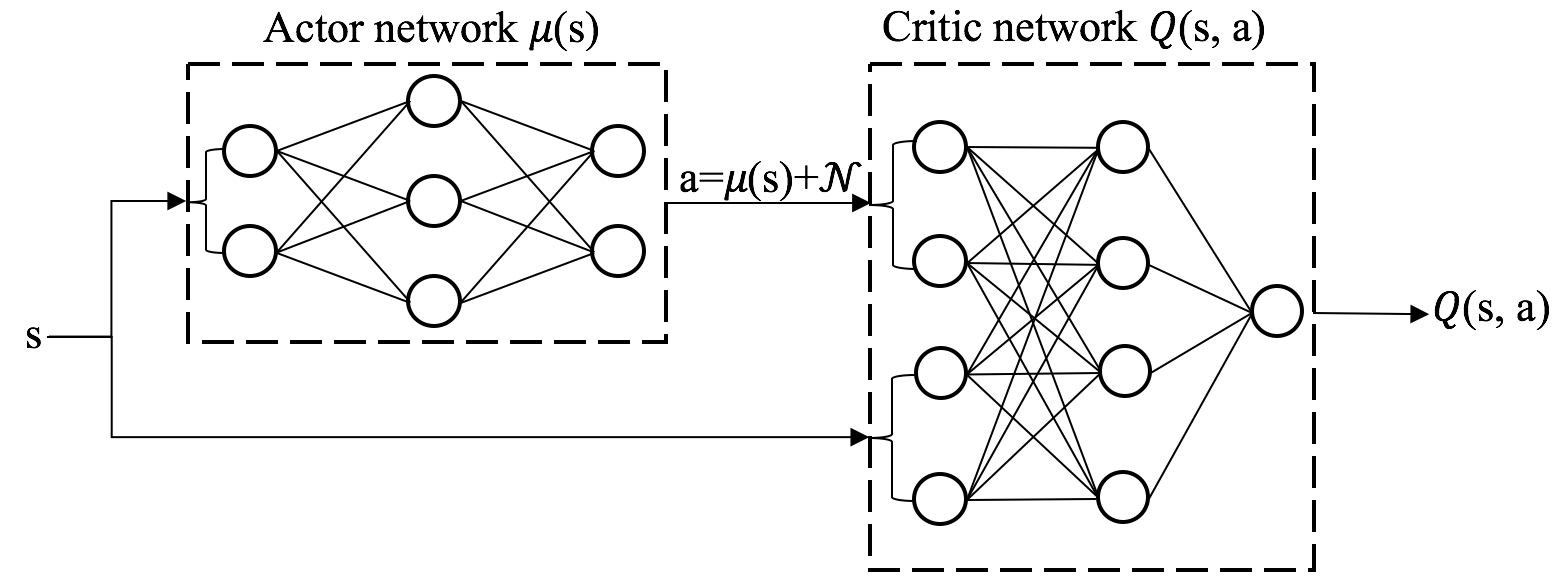
\includegraphics[width=0.8\textwidth]{actor-critic}
    \caption{Σχηματική αναπαράσταση των νευρωνικών δικτύων δράστη και κριτή}
    \label{fig:actor-critic}
\end{figure}

Φυσικά έχοντας αποφασίσει ποια θα είναι η δομή των δικτύων μας θα πρέπει να συνεχίζουμε με την εκπαίδευσή τους, δηλαδή τον προσδιορισμό των βέλτιστων παραμέτρων $\textbf{W}_{α}$ και $\textbf{W}_{c}$. Για τον σκοπό αυτόν θα χρειαστούμε φυσικά ένα κριτήριο βελτιστοποίησης και αυτό θα είναι η \textit{ελαχιστοποίηση μίας αντικειμενικής συνάρτησης} που θα επιβάλλουμε στον κριτή. Οι λεπτομέρειες της συνάρτησης αυτής θα παρουσιασθούν στο επόμενο κεφάλαιο, όπου θα παρουσιασθεί και θα περιγραφεί ο πλήρης αλγόριθμος DDPG. Ο λόγος είναι επειδή η συνάρτηση αυτή δεν περιέχει μονάχα τις παραμέτρους του δράστη και του κριτή αλλά και επιπλέον δύο διανύσματα παραμέτρων που αντιστοιχούν σε άλλα δύο νευρωνικά δίκτυα, τα λεγόμενα \textit{δίκτυα στόχους}.\\

\newpage

\section{Αλγόριθμος Deep Deterministic Policy Gradient}

\subsection{Εισαγωγή και Περιγραφή του Αλγορίθμου}
Έχοντας τώρα την θεωρία της Ενισχυτικής Μάθησης Βάθους θα παρουσιασθεί και θα επεξηγηθεί ο αλγόριθμος \cite{deepmind, stupidpaper, stupidpaper2} που θα επιλύσει το πρόβλημα της ρύθμισης. Ο πλήρης αλγόριθμος φαίνεται στον παρακάτω πίνακα:

\begin{table}[H]
\centering
\begin{tabular}{|p{0.3cm}|p{12cm}|}
\hline
\multicolumn{2}{|c|}{\textbf{Αλγόριθμος Εκμάθησης}} \\
\hline
1 & Αρχικοποίηση Δικτύων Δράστη και Κριτή \\
\hline
2 & Αρχικοποίηση Δικτύων Στόχου Δράστη και Κριτή\\
\hline
3 & Αρχικοποίηση Μνήμης Αναπαραγωγής \\
\hline
4  & \textbf{For episode = 1 to E do}: \\
\hline
5  & Επαναφορά (reset) θορύβου κατά Ornstein-Uhlenbeck $\aleph_t$  \\
\hline
6 & \textbf{For time step = 1 to T do} \\
\hline
7 & Παρατήρηση τρέχουσας κατάστασης $s = [y_t, y_{set}]$ \\
\hline
8 & Εκτέλεση Δράσης $α = u_t = \mu(s, W_α) + \aleph_t $\\
\hline
9 & Παρατήρηση επόμενης κατάστασης $s' = [y_{t+1}, y_{set}]$\\
\hline
10 & Λήψη αμοιβής $r_t$\\
\hline
11 & Αποθήκευση της τετράδας $[s, α, s', r]$ στην Μνήμη Αναπαραγωγής\\
\hline
12 & Λήψη τυχαίας παρτίδας $n$ τετράδων από την Μνήμη Αναπαραγωγής\\
\hline
13 & \textbf{For minibatch = 1 to $N$ do}: \\
\hline
14 & Υπολογισμός της ποσότητας $\phi_i = r_i + \gamma Q_t ^ i$ για κάθε τετράδα της παρτίδας\\
\hline
15 & Επικαιροποίηση του Κριτή : $W_c \leftarrow W_c - \alpha \nabla_{\textbf{W}_c} L(\textbf{W}_{c})$\\
\hline
16 & Υπολογισμός του $\nabla _p ^ i = \pdv{Q(s^i, α^i, W_c)}{α^i}$\\
\hline
17 & Αντιστροφή της βαθμίδας $\nabla _p ^ i$\\
\hline
18 & Επικαιροποίηση του Δράστη : $W_α \leftarrow W_α + \alpha \nabla_{\textbf{W}_α} \mathcal{J} (\textbf{W}_{α})$\\
\hline
19 & Επικαιροποίηση Δικτύου Στόχου Κριτή: $W_c ^ t \leftarrow \tau W_c + (1-\tau)W_c ^t$\\
\hline
20 & Επικαιροποίηση Δικτύου Στόχου Δράστη:  $W_α ^ t \leftarrow \tau W_α + (1-\tau)W_α ^t$\\
\hline
21 & \textbf{endfor}\\
\hline
22 & \textbf{endfor}\\
\hline
23 & \textbf{endfor}\\
\hline
\end{tabular}
\caption{Αλγόριθμος εκμάθησης μεθοδολογίας DDPG}
\label{table:1}
\end{table}

Θα προσπαθήσουμε τώρα να εξηγήσουμε βήμα-βήμα τον παραπάνω αλγόριθμο.\\

Πρώτο βήμα είναι η αρχικοποίηση των νευρωνικών δικτύων του δράστη, του κριτή και των αντίστοιχων δικτύων στόχων (τα δίκτυα στόχοι θα περιγραφούν παρακάτω) με τυχαία βάρη. Τα βάρη αυτά αρχικοποιούνται συνήθως σε μία περιοχή κοντά στο μηδέν για να αποφευχθούν τυχόν προβλήματα υπερχείλησης στα αρχικά στάδια της εκπαίδευσης. Σε αυτό επίσης βοηθά και η τεχνική της κανονικοποίησης κόστους (ενότητα \textbf{4.7}). Τα νευρωνικά δίκτυα αυτά θα δράσουν ώς συναρτησιακοί προσεγγιστές, όπως θα δούμε και στην συνέχεια. Επίσης αρχικοποιείται η μνήμη αναπαραγωγής. Αυτό σημαίνει ότι δημιουργούμε μία άδεια λίστα δεδομένης χωρητικότητας μέσα στην οποία θα αποθηκεύουμε τα αποτελέσματα της εκπαίδευσης.\\

Έχοντας τώρα έτοιμα τα νευρωνικά δίκτυα και την μνήμη αναπαραγωγής είμαστε έτοιμοι να εξηγήσουμε τις τρεις επαναληπτικές διαδικασίες (for-loops) του αλγορίθμου. Παρατηρούμε ότι η πρώτη επαναληπτική διαδικασία αφορά τα λεγόμενα \textit{επισόδεια}. Το κάθε επισόδειο αποτελείται από \textit{χρονικά βήματα}. Σε κάθε χρονικό βήμα εκτελούνται τα βήματα \textbf{7} έως \textbf{20} που φαίνονται στον πίνακα. Ο αριθμός των χρονικών βημάτων από τα οποία θα αποτελείται ένα επισόδειο ορίζεται από εμάς, όπως ακριβώς και ο αριθμός των επισοδείων που θα διαρκέσει η εκπαίδευση. Μόλις ο αριθμός των επισοδείων εξαντληθεί ο αλγόριθμος σταματά. Εναλλακτικά ο χρήστης μπορεί να τερματίσει τον αλγόριθμο όταν κρίνει ότι το πρόβλημα της βελτιστοποίησης έχει ολοκληρωθεί. Θα δούμε τώρα τα βήματα του αλγορίθμου που συντελούν ένα επισόδειο.\\

Αρχικά σχηματίζουμε το διάνυσμα της κατάστασης του συστήματος, \textbf{s}. Στον πίνακα φαίνεται ότι αυτό το διάνυσμα αποτελείται από δύο στοιχεία όμως σε μία πραγματική εφαρμογή το διάνυσμα αυτό μπορεί να αποτελείται από μέχρι και δεκάδες στοιχεία. Όσο πιο σύνθετος είναι ο χώρος των πιθανών καταστάσεων (δηλαδή όσο μεγαλύτερη διάσταση έχει) από τόσο περισσότερα στοιχεία θα αποτελείται και το διάνυσμα της κατάστασης. Στην συνέχεια εκτελούμε μία από τις πιθανές δράσεις, \textbf{\alpha} και μεταβαίνουμε στην επόμενη κατάσταση, η οποία αναπαριστάται από ένα διάνυσμα \textbf{s}' ίδιας διάστασης με την κατάσταση από την οποία προήλθε. Ταυτόχρονα ο πράκτορας λαμβάνει και μία αμοιβή, \textbf{r}, η οποία ορίζεται από την συνάρτηση κέρδους που έχει ορίσει ο χρήστης. Μέχρι το σημείο αυτό τα βήματα του αλγορίθμου συντελούν μία διαδικασία απόφασης κατά Markov. Στην συνέχεια τα δεδομένα (\textbf{s}, \textbf{\alpha}, \textbf{s}', \textbf{r}) αποθηκεύονται σε μία κενή θέση της μνήμης αναπαραγωγής. Στο σημείο αυτό κρίνεται σκόπιμο να αναφερθεί ότι μία από τις πιο σημαντικές παραμέτρους του αλγορίθμου είναι η συνάρτηση κέρδους $\textbf{r}(s, \alpha, s')$. Η επιλογή μίας τέτοιας συνάρτησης είναι πολύ λεπτό ζήτημα και μπορεί να κάνει την διαφορά στην εκπαίδευση. Μία συνάρτηση κέρδους μπορεί να οδηγεί σε ταχύτατη και αποδοτική εκπαίδευση ενώ κάποια άλλη ενδέχεται να αποτρέπει τον πράκτορα από το να προσεγγίζει την επιθυμητή κατάσταση.\\

Στην συνέχεια επιλέγουμε μία τυχαία παρτίδα δεδομένου μεγέθους από διανύσματα της μορφής (\textbf{s}, \textbf{\alpha}, \textbf{s}', \textbf{r}) από την μνήμη αναπαραγωγής. Εισερχόμαστε τώρα στην τρίτη και τελευταία επαναληπτική διαδικασία του αλγορίθμου. Για κάθε ένα από αυτά τα διανύσματα που πήραμε από την μνήμη αναπαραγωγής υπολογίζουμε την ποσότητα $\phi_{i} = r_{i} + \gamma Q^{i}_{t}$. Η ποσότητα αυτή μοιάζει πάρα πολύ με το εσωτερικό του αθροίσματος της εξίσωσης Bellman για την συνάρτηση $Q^{*}$ και όντως από εκεί πηγάζει η έμπνευση αυτή. Ονομάζεται \textit{στόχος} για λόγους που θα εξηγηθούν στην συνέχεια. Η ποσότητα $ Q^{i}_{t}$ είναι ένας πίνακας ακριβώς ίδιων διαστάσεων με τον γνωστό από την ενισχυτική μάθηση πίνακα $Q(s,\alpha)$. Παρόλα αυτά ο πίνακας αυτός δεν αποτελεί δεδομένο εξόδου του νευρωνικού δικτύου του κριτή. Αποτελεί έξοδο ενός επιπλέον νευρωνικού δικτύου, του \textit{Κριτή-Στόχου} (Target-Critic). Στο σημείο αυτό θα πρέπει να κάνουμε αλλαγή πορείας και να κάνουμε μία μικρή συζήτηση περί των δικτύων στόχων \cite{deepmind} που εμφανίζονται στα βήματα \textbf{2}, \textbf{19} και \textbf{20}.\\


\textbf{Δίκτυα-Στόχοι (Target Networks)}: Τα δίκτυα στόχοι έχουν ακριβώς ίδια δομή με αντίστοιχα δίκτυα δράστη και κριτή. Η κρίσιμη διαφορά είναι ότι έχουν διαφορετικές παραμέτρους, δηλαδή διαφορετικά βάρη και biases. Συμβολίζουμε με $\textbf{W}_{α}^{t}$ το διάνυσμα των παραμέτρων του νευρωνικού δικτύου του δράστη-στόχου και με $\textbf{W}_{c}^{t}$ το διάνυσμα των παραμέτρων του κριτή-στόχου. Η εισαγωγή των δικτύων-στόχων στον αλγόριθμο DDPG έχει μία θετική συνέπεια. Κατ'αρχάς καθιστά τον αλγόριθμο \textit{off-policy} \cite{deepmind}. Αυτό γιατί χρησιμοποιούνται διαφορετικά σετ παραμέτρων, τα $\textbf{W}_{α}$ και $\textbf{W}_{c}$, για τον υπολογισμό των συναρτήσεων $\mu(s)$ και $Q(s,\alpha)$ και διαφορετικά, τα $\textbf{W}_{α}^{t}$ και $\textbf{W}_{c}^{t}$, για την επικαιροποίηση των δικτύων του δράστη και του κριτή. Ο διαχωρισμός αυτός έχει δείξει εμπειρικά ότι καθιστά την εκμάθηση πολύ πιο σταθερή \cite{atari}. Ας υποθέσουμε ότι δεν υπήρχαν τα δίκτυα στόχοι. Τότε σε κάθε χρονικό βήμα οι παράμετροι του κριτή, $\textbf{W}_{c}$, θα χρησιμοποιούνταν για να αλλάξουν το ίδιο το δίκτυο (και άρα και τις παραμέτρους) του κριτή. Αυτού του είδους επικαιροποίηση μπορεί να προκαλέσει πολύ εύκολα αποκλίσεις, δηλαδή πολύ μεγάλου μέτρου βαθμίδες, κάτι που μπορεί να οδηγήσει σε αποσταθεροποίηση των δικτύων μας. Για τον λόγο αυτόν εισάγουμε τα δίκτυα στόχους. Παρόλα αυτά, ακριβώς επειδή δεν θέλουμε οι παράμετροί τους να ταυτίζονται με τις παραμέτρους των κανονικών δικτύων, η επικαιροποίησή τους γίνεται με πολύ πιο αργό ρυθμό. Για να υλοποιήσουμε αυτήν την χρονική υστέρηση των παραμέτρων των δικτύων-στόχων εισάγουμε άλλη μία παράμετρο η οποία ονομάζεται \textit{ρυθμός εκμάθησης των δικτύων-στόχων} και την συμβολίζουμε με $\tau$. Ο κανόνας επικαιροποίησης των παραμέτρων-στόχων είναι ο εξής:\\
\begin{gather}
\textbf{W}_c ^ t \leftarrow \tau \textbf{W}_c + (1-\tau)\textbf{W}_c ^t\\
\textbf{W}_α ^ t \leftarrow \tau \textbf{W}_α + (1-\tau) \textbf{W}_α ^t
\end{gather}

Φυσικά $0 < \tau \ll 1$. Θα δούμε τώρα πώς αυτές οι παράμετροι-στόχοι χρησιμοποιούνται για να επικαιροποιήσουν τις παραμέτρους του δράστη και του κριτή. Συνεχίζουμε με την περιγραφή του αλγορίθμου.\\

Τα επόμενα βήματα \textbf{15}-\textbf{18} είναι στην ουσία η καρδιά του προβήματος και του αλγορίθμου και αφορούν την επικαιροποίηση των παραμέτρων (βάρη και biases) του κριτή και του δράστη. Όπως είχε αναφερθεί στο κεφάλαιο \textbf{7} στους αλγορίθμους τύπου Δράστη-Κριτή ο κριτής ανανεώνει τις παραμέτρους του χρησιμοποιώντας κάποιον αλγόριθμο βελτιστοποίησης, όπως gradient descent, έτσι ώστε να ελαχιστοποιήσει την συνάρτηση κόστους που του έχουμε επιβάλλει και στην συνέχεια ο δράστης χρησιμοποιεί τις καινούριες αυτές παραμέτρους του κριτή έτσι ώστε να ανανεώσει τις δικές του παραμέτρους σύμφωνα με την βαθμίδα της συνάρτησης Q, αυτήν την φορά με gradient ascent, εφόσον στόχος μας είναι η μεγιστοποίηση της συνάρτησης αυτής. Η αντικειμενική συνάρτηση του κριτή είναι η εξής \cite{deepmind, stupidpaper2}\\
\begin{align*}
\displaystyle L(\textbf{W}_{c}) = \mathbb{E} \left[r + \gamma Q_{t}  - Q \right] ^ {2} =  \frac{1}{N} \sum_{i=1}^{N} \left(\phi_{i} - Q(s_{i}, \alpha_{i}; \textbf{W}_c) \right) ^ {2} 
\end{align*}
ή\\
\begin{equation}
\displaystyle L(\textbf{W}_{c}) = \frac{1}{N} \sum_{i=1}^{N} \left( r_{i}(s, \alpha, s') + \gamma Q(s_{i}', \mu(s_{i}', \textbf{W}_α ^ t); \textbf{W}_c ^ t) - Q(s_{i}, \alpha_{i}; \textbf{W}_{c}) \right) ^ {2}
\end{equation}
όπου $s'$ αναφέρεται στην κατάσταση του συστήματος που βρέθηκε ο πράκτορας μετά την λήψη της δράσης \alpha. Αν παρατηρήσουμε τον όρο που βρίσκεται μέσα στο άθροισμα της παραπάνω εξίσωσης θα διαπιστώσουμε ότι πρόκειται για \textit{χρονική διαφορά} (temporal difference), που παρουσιάσθηκε στην ενότητα \textbf{6.3}. Η συνάρτηση $\mu(s', \textbf{W}_α ^ t)$ είναι η ντετερμινιστική συνάρτηση πολιτικής-στόχος η οποία έχει προκύψει από το νευρωνικό δίκτυο του δράστη-στόχου. Η μόνη διαφορά με το κανονικό δίκτυο του δράστη είναι ότι σαν είσοδος αυτήν την φορά είναι η κατάσταση $s'$ και όχι η κατάσταση $s$. $N$ είναι το μέγεθος της παρτίδας που λάβαμε από την μνήμη αναπαραγωγής. Ο στόχος $\phi_{i}$ είναι σχεδόν ίδιος με το εσωτερικό του αθροίσματος της εξίσωσης Bellman για την συνάρτηση Q. Η κρίσιμη διαφορά είναι ότι εδώ δεν παίρνουμε κάποιο μέγιστο ως προς τις δράσεις. Αυτό συμβαίνει επειδή στα προβλήματα ρύθμισης ο χώρος των δράσεων είναι \textit{συνεχής} οπότε το μέγιστο δεν έχει ιδιαίτερο νόημα \cite{stupidpaper2}. Αντί αυτού σε κάθε χρονικό βήμα του αλγορίθμου κάνουμε μία βελτιστοποίηση ελαχιστοποιώντας την διαφορά μεταξύ της τρέχουσας συνάρτησης $Q(s,\alpha)$ που προέκυψε από τον κριτή και του στόχου, δηλαδή της βέλτιστης λύσης που θα μας έδινε η εξίσωση Bellman αν ο χώρος ήταν διακριτός. Η βαθμίδα της παραπάνω συνάρτησης ως προς τις παραμέτρους του δικτύου είναι η
\begin{equation}
\nabla_{\textbf{W}_c} L(\textbf{W}_{c}) = \mathbb{E} \left[(r + \gamma Q_{t} - Q(s,\alpha; \textbf{W}_c)) \nabla_{\textbf{W}_c} Q(s,\alpha, \textbf{W}_c) \right]
\end{equation}

Έπειτα κάνουμε επικαιροποίηση των παραμέτρων (βαρών) του νευρωνικού δικτύου του κριτή με βάση τον αλγόριθμο mini-batch Gradient Descent με την χρήση ενός βελτιστοποιητή (optimizer) του Tensorflow, όπως φαίνεται στο βήμα \textbf{15} του αλγορίθμου. Σημειώνεται εδώ ότι ο συμβολισμός $\nabla_{\textbf{W}_c} L(\textbf{W}_{c})$ σημαίνει μερική παραγώγιση ως προς όλες τις παραμέτρους του δικτύου (βάρη και biases). Συνέχεια έχει η επικαιροποίηση των παραμέτρων του δράστη. Όπως περιγράφηκε στο κεφάλαιο \textbf{6} χρησιμοποιούμε τις επικαιροποιημένες παραμέτρους του κριτή έτσι ώστε να υπολογίσουμε την βαθμίδα που δίνεται από την εξίσωση (6.2.1). Αν δηλαδή συμβολίσουμε με $\mathcal{J}(\textbf{W}_α) = \mathbb{E}\left[Q(s,\alpha; \textbf{W}_α) \right]$ την αντικειμενική συνάρτηση του δράστη τότε από το Θεώρημα Βαθμίδας Ντετερμινιστικής Πολιτικής \cite{dpga} παίρνουμε
\begin{equation}
\nabla_{\textbf{W}_α} \mathcal{J}(\textbf{W}_α) = \mathbb{E} \left[ \nabla_{\textbf{W}_α} \mu(s, \textbf{W}_α) \nabla_{α} Q(s,\alpha; \textbf{W}_α) |_{α = \mu(s)} \right]
\end{equation}

Στην συνέχεια, όπως φαίνεται στο βήμα \textbf{18} του αλγορίθμου, οι παράμετροι του δράστη επικαιροποιούνται με βάση τον αλγόριθμο mini-batch gradient ascent, προκειμένου να μεγιστοποιηθεί η συνάρτηση $\mathbb{E}[Q]$, η οποία όπως ξέρουμε από το κεφάλαιο της ενισχυτικής μάθησης είναι άμεσα συνδεδεμένη με το κέρδος του πράκτορα. Τα τελευταία δύο βήματα του αλγορίθμου, \textbf{19} και \textbf{20}, αποτελούν την επικαιροποίηση των δίκτυων-στόχων. Κλείσαμε έτσι ένα χρονικό βήμα του αλγορίθμου. Η διαδικασία αυτή επαναλαμβάνεται για όσα χρονικά βήματα έχουμε θέσει να διαρκεί ένα επισόδειο και για όσα επισόδεια έχουμε θέσει να διαρκέσει ο αλγόριθμος. Φυσικά ο αλγόριθμος σταματά όταν έχουν εξαντληθεί όλα τα επισόδεια ή όταν ο χρήστης σταματήσει χειροκίνητα τον αλγόριθμο, όταν κρίνει ότι μόνιμη κατάσταση έχει επιτευχθεί και ότι ο αλγόριθμος έχει συγκλίνει.\\

Στην συνέχεια θα εξετάσουμε λίγο πιο λεπτομερώς κάποια πιο τεχνικά σημεία του αλγορίθμου, δηλαδή την λειτουργία της μνήμης αναπαραγωγής, τον θόρυβο κατά Ornstein-Uhlenbeck που φαίνεται στα βήματα \textbf{5} και \textbf{8}, την τεχνική της \textit{κανονικοποίησης παρτίδας}, μίας τεχνικής που χρησιμοποιείται κατά κόρον σε προβλήματα με μεγάλο αριθμό δεδομένων αλλά και σε πολλές εφαρμογές νευρωνικών δικτύων, και την τεχνική της \textit{αντιστροφής βαθμίδας}, δηλαδή το βήμα \textbf{17} του αλγορίθμου για το οποίο δεν έγινε καμία αναφορά.\\

\subsection{Μνήμη Αναπαραγωγής (Replay Memory)}

Όπως φαίνεται στον πίνακα του αλγορίθμου, σε κάθε time step ενός επισοδείου αποθηκεύουμε την πληροφορία που πήραμε από την λήψη της δράσης στο συγκεκριμένο βήμα στην λεγόμενη \textit{μνήμη αναπαραγωγής} (replay memory). Η πληροφορία αυτή αποτελείται από το τετράνυσμα $(s_t, \alpha_t, s_{t + 1}, r_t)$, δηλαδή από την κατάσταση στην οποία βρισκόμαστε στο συγκεκριμένο time step, $s_t$, την δράση που έλαβε ο δράστης, $\alpha_t$, την κατάσταση στην οποία βρέθηκε ο πράκτορας μετά την λήψη της δράσης, $s_{t + 1}$, και την αμοιβή που έλαβε ο πράκτορας, $r_t$. Το τετράνυσμα αυτό καλείται μία \textit{εμπειρία} (experience). Η εμπειρία αυτή που σχηματίζεται σε κάθε time step αποθηκεύεται σε μία εικονική λίστα δεδομένης χωρητικότητας, η οποία στην αρχή του αλγορίθμου αρχικοποιείται άδεια. Όσο η λίστα αυτή γεμίζει με εμπειρίες η εκπαίδευση των νευρωνικών μας δικτύων (δηλαδή τα βήματα του αλγορίθμου που ακολουθούν) διεκπεραιώνεται με βάση αυτές τις υπάρχουσες εμπειρίες.  Πιο συγκεκριμένα, σε κάθε time step επιλέγουμε μία τυχαία παρτίδα (mini-batch) συγκεκριμένου μεγέθους εμπειριών από την μνήμη αναπαραγωγής και τις χρησιμοποιούμε για να εκπαιδεύσουμε τα δίκτυά μας. Η τεχνική αυτή έχει ένα μεγάλο πλεονέκτημα σε σύγκριση με το αν χρησιμοποιούσαμε διαδοχικές εμπειρίες (για παράδειγμα τις τελευταίες 64 εμπειρίες) του πράκτορα. Επιλέγοντας τυχαίες εμπειρίες της μνήμης πετυχαίνουμε την \textit{άρση της αυτοσυσχέτισης} μεταξύ διαδοχικών δειγμάτων \cite{replaymemory}. Αν τα δίκτυα εκπαιδεύονταν από δείγματα διαδοχικών εμπειριών που προέκυπταν από την εξερεύνηση του περιβάλλοντος τότε τα δείγματα αυτά θα συσχετίζονταν μεταξύ τους όλο και πιο πολύ όσο συνεχιζόταν η εκπαίδευση. Η τυχαιότητα των δειγμάτων σπάει ακριβώς αυτήν την συσχέτιση.\\

Στο σήμειο αυτό θα πρέπει να αναφερθούν δύο σημαντικές λεπτομέρειες της εν λόγω τεχνικής. Καταρχάς αναφέρθηκε πως σε κάθε time step επιλέγουμε μία τυχαία παρτίδα εμπειριών δεδομένου μεγέθους. Παρόλα αυτά η μνήμη αρχικοποιείται άδεια που σημαίνει ότι στα αρχικά στάδια της εκπαίδευσης δεν υπάρχουν αρκετές εμπειρίες για να πάρουμε δείγμα. Το πρόβλημα αυτό λύνεται εισάγοντας τον λεγόμενο \textit{χρόνο προθέρμανσης} (warm-up time) \cite{warmuptime}. Κατά την διάρκεια του χρόνου αυτού \textit{δεν} εκπαιδεύουμε τα νευρωνικά μας δίκτυα αλλά το μόνο που κάνουμε είναι να γεμίζουμε την μνήμη αναπαραγωγής με τυχαίες εμπειρίες. Για να τοποθετηθούμε λίγο καλύτερα στο πρόβλημα, κατά τον χρόνο προθέρμανσης τρέχουμε τον αλγόριθμό μας μέχρι το βήμα \textbf{11}, δηλαδή μέχρι ακριβώς πριν την έναρξη της εκπαίδευσης των νευρωνικών δικτύων. Ο χρόνος προθέρμανσης μπορεί να διαρκεί έως και αρκετά επισόδεια και συνήθως τελειώνει μόλις γεμίσει πλήρως η μνήμη αναπαραγωγής. Με την μνήμη μας γεμάτη εμπειρίες μπορεί να αρχίσει η εκπαίδευσης. Τώρα όμως έχει δημιουργηθεί ένα δεύτερο πρόβλημα που καλούμαστε να λύσουμε. Εφόσον η μνήμη έχει γεμίσει με εμπειρίες τυχαίες, οι οποίες δεν έχουν προκύψει από κάποια λογική συνέχεια ή εξερεύνηση του χώρου (και άρα θα είναι πρακτικά άχρηστες για την εκπαίδευση) και οι παρτίδες που θα επιλέγουμε θα αποτελούνται καθαρά και μόνο από αυτές τις ανούσιες εμπειρίες, αναμένουμε πως η εκπαίδευση θα είναι ανεπιτυχής. Για τον λόγο αυτόν κάνουμε το εξής κόλπο: μόλις γεμίσει πλήρως η μνήμη αναπαραγωγής τότε προκειμένου να βάλουμε την επόμενη εμπειρία στην μνήμη \textit{αφαιρούμε} το πρώτο στοιχείο της μνήμης (αυτό δηλαδή που βρίσκεται στην θέση 0, στο αριστερό άκρο της μνήμης). Με αυτόν τον τρόπο και έχοντας αρχίσει η εκπαίδευση των νευρωνικών δικτύων η μνήμη θα γεμίζει με όλο και καλύτερες εμπειρίες ενώ παράλληλα θα αφαιρούνται οι τυχαίες και άχρηστες εμπειρίες των αρχικών σταδίων του χρόνου προθέρμανσης.


\subsection{Θόρυβος Ornstein - Uhlenbeck}
Όπως φαίνεται στον κεντρικό αλγόριθμο της μεθοδολογίας DDPG, η δράση $\alpha_t$ αποτελείται από δύο κομμάτια. Το ένα κομμάτι είναι η προς προσδιορισμό συνάρτηση πολιτικής, $\pi$. Το δεύτερο κομμάτι αποτελεί τον αποκαλούμενο \textit{Θόρυβο κατά Ornstein - Uhlenbeck}. Για να καταλάβουμε ακριβώς περι τίνος πρόκειται και για ποιόν λόγο χρησιμοποιείται στον αλγόριθμό μας θα πρέπει να εισάγουμε την έννοια της \textit{διαδικασίας κατά Wiener} ή της λεγόμενης \textit{κίνησης κατά Brown}.\\

\textbf{Ορισμός}: Μία \textit{(μονοδιάστατη) διαδικασία κατά Wiener} (γνωστή και ως \textit{κίνηση κατά Brown}) είναι μία στοχαστική διαδικασία $\{W_t\}_{t \geq 0+}$ με δείκτες τους μη-αρνητικούς πραγματικούς αριθμούς $t$ με τις εξής ιδιότητες:
\begin{itemize}
  \item $W_0 = 0$
  \item Η συνάρτηση που ορίζεται από την απεικόνιση $t$ $\rightarrow$ $W_t$ είναι συνεχής ως προς την μεταβλητή $t$ με πιθανότητα 1, με την έννοια ότι $\displaystyle \mathbb{P}\left(\limsup\limits_{\epsilon \rightarrow 0} \sup_{0 \leq s < t \leq 1, t - s \leq \epsilon} \frac{\abs{W(s) - W(t)}}{\sqrt{2 \epsilon \log \log (1/\epsilon)}} = 1\right) = 1$
  \item Η διαδικασία $\{W_t\}_{t \geq 0+}$ έχει ανεξάρτητες από το παρελθόν προσαυξήσεις. Αυτό σημαίνει ότι για κάθε $t > 0$ οι διαφορές $W_{t + u} - W_t$, με $u > 0$ είναι ανεξάρτητες των παλαιότερων τιμών $W_s$ με $s < t$.
  \item $W_{t + u} - W_t$ $\sim$ $\mathcal{N}$(0,u). 
\end{itemize}

Η συνάρτηση $W_t$ έχει δύο (μεταξύ άλλων) πολύ ενδιαφέρουσες ιδιότητες. Καταρχάς πρόκειται για μια συνάρτηση που παρόλο που είναι παντού συνεχής δεν είναι πουθενά παραγωγίσιμη. Επιπλέον, αν υποθέσουμε ότι η $\{X_i\}$ είναι μία οικογένεια ανεξάρτητων και ομοίως κατανεμημένων τυχαίων μεταβλητών με μέση τιμή 0 και διασπορά 1, μπορούμε τότε για  κάθε $n$ να ορίσουμε την συνεχή στοχαστική διαδικασία:\\
\begin{align*}
W_n (t) = \frac{1}{\sqrt{n}} \sum_{1 \leq k \leq \left \lfloor{nt}\right \rfloor } X_i, \hspace{1cm} t \in [0, 1]
\end{align*}

Η παραπάνω διαδικασία είναι γνωστή και ως \textit{τυχαίος περίπατος}. Εφόσον οι τυχαίες μεταβλητές $X_i$ είναι ανεξάρτητες και οι προσαυξήσεις της $W_n$ θα είναι ανεξάρτητες. Από το κεντρικό οριακό θεώρημα, καθώς $n \rightarrow \infty$ έχουμε ότι $W_n (t) - W_n (s)$ $\sim$ $\mathcal{N}$(0, t - s). Επίσης από το θεώρημα του Donsker καθώς $n \rightarrow \infty$ η $W_n$ προσεγγίζει μία διαδικασία κατά Wiener. \\

Έχοντας την έννοια και την μορφή μίας συνάρτησης τυχαίου περιπάτου είμαστε έτοιμη να δώσουμε την στοχαστική διαφορική εξίσωση που περιγράφει την διαδικασία Ornstein-Uhlenbeck, $X_t$ \cite{ounoise}. Αυτή είναι η παρακάτω:\\
\begin{equation}
dX_t = -\theta(\mu - X_t)dt + \sigma dW_t
\end{equation}

Πρόκειται δηλαδή για μία στοχαστική διαδικασία η οποία καθορίζεται τελικά από έναν τυχαίο περίπατο (κίνηση κατά Brown). Οι παράμετροι $\theta$, $\mu$ και $\sigma$ περιγράφουν το είδος του τυχαίου περιπάτου. Η παράμετρος $\theta$ είναι ενδεικτική του πόσο ισχυρά το σύστημά μας αντιδρά σε διαταραχές, η παράμετρος $\sigma$ δείχνει την διασπορά ή το μέγεθος του θορύβου και η παράμετρος $\mu$ είναι ο ασυμπτωτικός μέσος όρος. Η παραπάνω διαφορική εξίσωση λύνεται και παίρνουμε την εξής λύση: \\
\begin{equation}
X_t = \alpha + (x_0 - \alpha) e^{-\beta t} + \sigma \int_{0}^{t} e^{-\beta (t - s)} dW_s
\end{equation}

Ο λόγος που προστίθεται ο όρος αυτού του τυχαίου περιπάτου στην δράση $\alpha_t$ είναι επειδή επιτρέπει στον πράκτορα να εξερευνήσει τον (συνεχές) χώρο καταστάσεων με μεγαλύτερη ταχύτητα και απόδοση ακριβώς λόγω της τυχαιότητας που κληρονομεί η δράση από τον θόρυβο αυτόν. Εμπειρικά η εισαγωγή αυτού του είδος θορύβου στην μεθοδολογία του DDPG έχει δείξει ότι αυξάνει τους ρυθμούς εκπαίδευσης του πράκτορα \cite{deepmind}.\\

\subsection{Κανονικοποίηση Παρτίδων (Batch Normalization)}

Ένα ακόμη τέχνασμα που έχει εμπειρικά δείξει ότι αυξάνει σημαντικά την απόδοση και την ταχύτητα της εκπαίδευσης νευρωνικών δικτύων βάθους είναι αυτό της \textit{κανονικοποίησης παρτίδων}. Για να καταλάβουμε περί τίνος πρόκειται και πώς υλοποιείται θα πρέπει πρώτα να καταλάβουμε ποιο είναι εκείνο το πρόβλημα που καλείται να επιλύσει. Εν γένει η εκπαίδευση νευρωνικών δικτύων με πολλαπλά κρυφά στρώματα παρουσιάζει την εξής δυσκολία: κατά την διάρκεια της εκπαίδευσης οι παράμετροι (δηλαδή τα βάρη και τα biases) αλλάζουν συνεχώς. Αυτό έχει ως αποτέλεσμα η κατανομή των δεδομένων που εισέρχονται σε μία βαθμίδα να αλλάζει και αυτή καθ'όλη την διάρκεια της εκπαίδευσης. Αυτή η συνεχής αλλαγή οδηγεί σε πολύ μικρούς ρυθμούς εκπαίδευσης, εφόσον το κάθε στρώμα θα πρέπει κάθε φορά να προσαρμόζεται σε μία νέα κατανομή και απαιτεί πολύ προσεχτική αρχικοποίηση των παραμέτρων. Το φαινόμενο αυτό καλείται \textit{εσωτερική μεταβλητή μετατόπιση} (internal covariate shift) \cite{batchnorm}. Για να λυθεί το συγκεκριμένο πρόβλημα χρησιμοποιούμε έναν αλγόριθμο κανονικοποίησης των δεδομένων ο οποίος μας εγγυάται ότι τα δεδομένα εισόδου σε κάθε κρυφό στρώμα θα έχουν συνεχώς μία σταθερή κατανομή και συνεπώς θα μειωθεί σημαντικά η εσωτερική μεταβλητή μετατόπιση. Πιο συγκεκριμένα φροντίζουμε έτσι ώστε τα δεδομένα που εισέρχονται σε ένα κρυφό στρώμα να έχουν μέση τιμή 0 και διασπορά 1. Ο μετασχηματισμός που θα πετύχει αυτές τις συνθήκες είναι ο εξής: Αν $x$ είναι η είσοδος ενός νευρώνα ενός κρυφού στρώματος τότε η \textit{κανονικοποιημένη είσοδος}, έστω $\hat{x}$ θα δίνεται από την σχέση:\\
\begin{align*}
\hat{x} = \frac{x - \mathbb{E}(x)}{Var(x)}
\end{align*}

Όπως θα δείξουμε σε λίγο οι μετασχηματισμένες αυτές ποσότητες έχουν όντως μέση τιμή ίση με το 0 και διασπορά 1. Επίσης να παρατηρήσουμε ότι αν η είσοδος του στρώματος αποτελείται από ένα $n$-διάστατο διάνυσμα $x = \left(x_1, x_2, \dots, x_n \right)$, τότε απλώς κανονικοποιούμε την κάθε διάσταση ξεχωριστά:
\begin{align*}
\hat{x}^i  = \frac{x^i - \mathbb{E}(x^i)}{Var(x^i)}
\end{align*}

Στο σημείο αυτό θα πρέπει να παρατηρήσουμε ότι ένας τέτοιος μετασχηματισμός μπορεί να προκαλέσει ένα όχι και τόσο προφανές πρόβλημα. Αν μία κανονικοποιημένη τιμή εισόδου εισέλθει σε μία σιγμοειδή καμπύλη προς επεξεργασία τότε αυτή ωθείται προς την γραμμική περιοχή (σε περιοχές κοντά στο 0), κάτι το οποίο δεν θέλουμε καθώς όπως έχει εξηγηθεί ήδη οι γραμμικές συναρτήσεις δεν είναι κατάλληλες για εκπαίδευση νευρωνικών δικτύων. Για να αντιμετωπίσουμε το πρόβλημα αυτό σε κάθε μεταβλητή $x^i$ αντιστοιχίζουμε ένα ζεύγος παραμέτρων $\gamma^i$ και $\beta^i$ και εφαρμόζουμε έναν ακόμα μετασχηματισμό:
\begin{align*}
\hat{x}^i \rightarrow \gamma^i \hat{x}^i + \beta^i = \hat{y}^i
\end{align*} 

Οι παράμετροι $\gamma^i$ και $\beta^i$ προσδιορίζονται και αυτοί κατά την διάρκεια της εκπαίδευσης, όπως ακριβώς και τα βάρη και τα biases του νευρωνικού δικτύου.\\

Ας υποθέσουμε τώρα ότι κατά την διάρκεια της εκπαίδευσης χρησιμοποιούμε παρτίδες (mini-batches) δεδομένων που ενδεχομένως να αντλούνται από κάποια μνήμη αναπαραγωγής. Έστω ότι οι παρτίδες αυτές έχουν μέγεθος $m$. Συνεπώς για έναν νευρώνα ενός κρυφού στρώματος (έστω ότι πρόκειται για τον νευρώνα $i$)  θα έχουμε μία παρτίδα $m$ δεδομένων εισόδου $ \mathcal{B} = \{x_k^i\}_{k=1}^m$. Κάθε τέτοια παρτίδα θα έχει μία μέση τιμή, $\mu_{\mathcal{B}}$ και μία διασπορά $\sigma_{\mathcal{B}}$ που θα δίνονται από την σχέση:
\begin{align*}
\mu_{\mathcal{B}} = \frac{1}{m} \sum_{k=1}^{m} x_k^i\\
\sigma_{\mathcal{B}} = \frac{1}{m} \sum_{k=1}^{m} (x_k^i -\mu_{\mathcal{B}} )^2
\end{align*}

Έχοντας τις παραπάνω τιμές της μέσης τιμής και της διασποράς της παρτίδας εφαρμόζουμε διαδοχικά τους παρακάτω ματασχηματισμούς:
\begin{align*}
x_k^i \rightarrow \frac{x_k^i - \mu_{\mathcal{B}}}{\sqrt{\sigma_{\mathcal{B}} + \epsilon}} = \hat{x}_k^i\\
\hat{x}_k^i \rightarrow \gamma_k^i \hat{x}_k^i + \beta_k^i = \hat{y}_k^i
\end{align*}

Ο αριθμός $\epsilon$ είναι μία πολύ μικρή παράμετρος ($0 < \epsilon << 1$) και την εισάγουμε μόνο για λόγους αριθμητικής ευστάθειας. Το μόνο που θα πρέπει να δείξουμε τώρα είναι πως πράγματι η μέση τιμή και η διασπορά των μετασχηματισμένων εισόδων $\hat{x}_k^i$ παίρνουν τις επιθυμητές τιμές, δηλαδή 0 και 1 αντίστοιχα. Αρχίζουμε με την μέση τιμή:
\begin{align*}
\mathbb{E}(\hat{x}_k^i) = \mathbb{E}\left( \frac{x_k^i - \mu_{\mathcal{B}}}{\sqrt{\sigma_{\mathcal{B}} + \epsilon}}\right) = \frac{1}{\sqrt{\sigma_{\mathcal{B}} + \epsilon}} \mathbb{E} (x_k^i - \mu_{\mathcal{B}}) = \frac{1}{\sqrt{\sigma_{\mathcal{B}} + \epsilon}} (\mathbb{E}(x_k^i) - \mathbb{E}(\mu_{\mathcal{B}})) =  \\
\frac{1}{\sqrt{\sigma_{\mathcal{B}} + \epsilon}} (\mu_{\mathcal{B}} - \mu_{\mathcal{B}}) = 0\\
\end{align*}

\begin{align*}
\sigma(\hat{x}_k^i) =   \mathbb{E}[(\hat{x}_k^i)^2] - (\mathbb{E}[\hat{x}_k^i])^2  =  \mathbb{E}[(\hat{x}_k^i)^2] = \mathbb{E}\left( \frac{(x_k^i)^2 + (\mu_{\mathcal{B}})^2 - 2x_k^i \mu_{\mathcal{B}}}{\sigma_{\mathcal{B}} + \epsilon}\right) =\\
 \frac{1}{\sigma_{\mathcal{B}} + \epsilon} \left(\mathbb{E}[(x_k^i)^2] + \mathbb{E}((\mu_{\mathcal{B}})^2) - 2\mu_{\mathcal{B}} \mathbb{E}[x_k^i]\right) =  \frac{1}{\sigma_{\mathcal{B}} + \epsilon} \left(\mathbb{E}[(x_k^i)^2] + (\mu_{\mathcal{B}})^2 - 2(\mu_{\mathcal{B}})^2\right) = \\
\frac{1}{\sigma_{\mathcal{B}} + \epsilon} \left(\mathbb{E}[(x_k^i)^2] - (\mu_{\mathcal{B}})^2\right) = \\
\frac{\sigma_{\mathcal{B}}}{\sigma_{\mathcal{B}} + \epsilon}
\end{align*}

Έχοντας στο μυαλό μας ότι η παράμετρος $\epsilon$ είναι πάρα πολύ μικρή (και για πρακτικούς λόγους μπορεί να αγνοηθεί) παίρνουμε το ζητούμενο.

\subsection{Αντιστροφή Βαθμίδας (Gradient Inverter)}

Στις περισσότερες περιπτώσεις ρύθμισης μίας διεργασίας ο χώρος των δράσεων είναι ένα φραγμένο σύνολο αφού η κάθε δράση αντιστοιχεί σε μία ενέργεια που βεβαίως έχει μία φυσική σημασία (π.χ. ροή, θερμοκρασία κ.α.). Κατά την διάρκεια της εκπαίδευσης των νευρωνικών δικτύων, ένα αυστηρά μη-κυρτό πρόβλημα βελτιστοποίησης, οι βαθμίδες που υπολογίζονται μπορούν εύκολα να πάρουν πολύ μεγάλες τιμές και συνεπώς οι υπολογιζόμενες δράσεις να βγαίνουν αρκετά εκτός των επιτρεπόμενων ορίων. Για τον λόγο αυτό εισάγεται στον αλγόριθμο το βήμα \textbf{17}. Πρόκεται για τον εξής μετασχηματισμό \cite{gradinv}:

\begin{gather*}
\nabla_{p}
\rightarrow
\nabla_{p}
\left\{
\begin{array}{ll}
      \frac{p_{max}-p}{p_{max}-p_{min}} & αν \hspace{0.2cm} \nabla_{p} > 0 \\
      \frac{p-p_{min}}{p_{max}-p_{min}} & αλλιως \\
\end{array} 
\right.
\end{gather*}

Πρόκεται για έναν μετασχηματισμό κανονικοποίησης της δράσης. Όσο οι τιμές των δράσεων τείνουν προς τα άκρα του εκάστοτε διαστήματος στο οποίο ορίζονται οι βαθμίδες υποβαθμίζονται και αντιστρέφονται αν οι τιμές αυτές βγούν εκτός των άκρων αυτών. Η μέθοδος της αντιστροφής βαθμίδας δουλεύει με μεγαλύτερη επιτυχία σε μοντέλα όπου οι συναρτήσεις που περιλαμβάνονται είναι λείες (συνεχείς με άπειρης τάξης συνεχείς παραγώγους) και οι κλίσεις που εμφανίζονται δεν είναι ιδιαίτερα μεγάλες. Επίσης κρίνεται σκόπιμο να αναφερθεί ότι το βήμα αυτό του αλγορίθμου είναι προαιρετικό. Ο αρχικός αλγόριθμος της DeepMind που δημιουργήθηκε για να λύσει προβλήματα ρύθμισης δεν περιείχε αυτό το βήμα. Πρόκειται για μία τροποποίηση του αλγορίθμου που μας βοηθά να περιορίσουμε το εύρος των δράσεων.


\newpage

\section{Εφαρμογές και αποτελέσματα}

\subsection{Εφαρμογή της μεθοδολογίας DDPG σε γραμμικό μοντέλο μίας εισόδου και μίας εξόδου}
Ως πρώτο βήμα θα εφαρμόσουμε το προτεινόμενο μοντέλο ρύθμισης σε ένα γραμμικό σύστημα $1 \times 1$ το οποίο δανειστήκαμε από την βιβλιογραφία \cite{linearmodel}. Η συνάρτηση μεταφοράς που περιγράφει το σύστημα είναι η εξής :
\begin{equation}
G(s) = \frac{0.05}{s ^ 4 - 0.6  s ^ 3}
\end{equation}

Ο αντίστοιχος χώρος φάσεων περιγράφεται από τις γραμμικές εξισώσεις:
\begin{gather*}
\textbf{$\dot{x}$}
=
\begin{bmatrix} 0 & 1 & 0 & 0 \\ 0 & 0 & 1 & 0 \\ 0 & 0 & 0 & 1 \\ 0 & 0 & 0 & 0.6 \end{bmatrix}
\textbf{x}
+
\begin{bmatrix} 0 \\ 0 \\ 0 \\ 1 \end{bmatrix}
\textbf{u}
\end{gather*}
\begin{gather*}
\textbf{y}
=
\begin{bmatrix} 0.05 & 0 & 0 & 0 \end{bmatrix}
\textbf{x}
\end{gather*}
Το φυσικό σύστημα που περιγράφεται από τις παραπάνω εξισώσεις είναι μία διεργασία παραγωγής χαρτιού \cite{linearmodel}. Η έξοδος του συστήματος, \textbf{y}(t), είναι η ποσότητα υγρασίας στο χαρτί. Η είσοδος, \textbf{u}, είναι η ροή του ατμού που χρησιμοποιείται για να υγράνει το χαρτί. Σε γλώσσα ενισχυτικής μάθησης ορίζουμε σαν \textit{κατάσταση} (state) του συστήματος να είναι το διάνυσμα:
\begin{align*}
\textbf{s}(t) = (\textbf{y}(t), \textbf{y}_{set})
\end{align*}
δηλαδή το διάνυσμα που αποτελείται από την τρέχουσα έξοδο του συστήματος και το set point. Ο λόγος που η κατάσταση ορίζεται με αυτόν τον τρόπο είναι επειδή ο πράκτορας (στην ουσία ο ρυθμιστής) πρέπει σε κάθε χρονικό βήμα να γνωρίζει τόσο την τρέχουσα έξοδο του συστήματος όσο και τον τελικό στόχο του (set point) έτσι ώστε να μπορέσει να λάβει την κατάλληλη δράση. Την κατάσταση του συστήματος $\textbf{y}(t)$ την υπολογίζουμε λύνοντας σε κάθε χρονικό βήμα το παραπάνω γραμμικό σύστημα εξισώσεων με την χρήση της βιβλιοθήκης control της Python. \\

Η μεταβλητή εισόδου \textbf{u}(t) είναι η \textit{δράση} (action) που θα λαμβάνει ο πράκτορας σε κάθε χρονικό βήμα. Ακριβέστερα, με βάση την μεθοδολογία DDPG, η δράση θα ισούται με:
\begin{align*}
\textbf{\alpha}(t) = \textbf{u}(t) + \mathcal{N}(t) = \mu(t) + \mathcal{N}(t)
\end{align*}

όπου $ \mu(t)$ η ντετερμινιστική συνάρτηση πολιτικής και $\mathcal{N}(t)$ είναι ο θόρυβος κατά Ornstein-Uhlenbeck. Η λήψη μίας δράσης έχει ως αποτέλεσμα την μετάβαση του πράκτορα από την τρέχουσα κατάσταση στην επόμενη, την οποία θα συμβολίσουμε ως:

\begin{align*}
\textbf{s}'(t) = (\textbf{y}(t+1), \textbf{y}_{set})
\end{align*}

Στόχος μας είναι, ξεκινώντας από μηδενική τιμή υγρασίας να προσδιορίσουμε εκείνο το προφίλ της ροής του ατμού που θα φέρει το χαρτί μας σε μία κατάσταση επιθυμητής υγρασίας. Το μοντέλο αυτό το δανειστήκαμε από σχετική βιβλιογραφία. Δυστυχώς όμως στην βιβλιογραφία δεν παρατίθενται οι μονάδες μέτρησης τόσο της υγρασίας του χαρτιού όσο και της ροής του ατμού. Για τον λόγο αυτό θα φερθούμε στο σύστημα αυτό ως ένα αμιγώς μαθηματικό μοντέλο που θα αποτελέσει μία αρχική δοκιμασία της προτεινόμενης μεθοδολογίας. \\

Παρακάτω παρουσιάζονται διάφοροι παράμετροι του αλγορίθμου που επιλέχθηκαν για την προσομοίωση:\\

Η προσομοίωση υλοποιήθηκε σε γλώσσα προγραμματισμού Python, με την βοήθεια (μεταξύ άλλων) της βιβλιοθήκης Tensorflow. Ο κώδικας που χρησιμοποιήθηκε είναι στο ίδιο στυλ με αυτόν που υπάρχει στην πρώτη ηλεκτρονική παραπομπή στο τέλος του κειμένου. Όσον αφορά τα νευρωνικά δίκτυα του δράστη, του κριτή αλλά και τα αντίστοιχα δίκτυα-στόχους και τα τέσσερα αποτελούνται από δύο κρυφά στρώματα. Το πρώτα κρυφό στρώμα έχει 400 κόμβους (νευρώνες) και το δεύτερο 300. Όλες οι συναρτήσεις ενεργοποίησης επιλέχθηκαν να είναι της μορφής ReLU. Ο ρυθμός εκμάθησης είναι κοινός για όλα τα δίκτυα και είναι ίσος με $5 \cdot 10^{-4}$. Τα δίκτυα-στόχοι ανανεώνονται με βάση τα βήματα \textbf{19} και \textbf{20} με $\tau = 10^{-3}$. Σε όλες τις παραμέτρους του νευρωνικού δικτύου του κριτή επιβάλλουμαι και ένα επιπλέον $\mathcal{L}^2$-κόστος (με πολλαπλασιαστική σταθερά ίση με 0.5). Στην δράση προστέθηκε και θόρυβος κατά Ornstein-Uhlenbeck με σταθερές $\mu = 0, \theta = 0.15, \sigma = 0.2$. Ο παράγοντας προεξόφλησης $\gamma$ τίθεται ίσος με 0.99.  Στην μνήμη αναπαραγωγής δόθηκε χωρητικότητα ίση με $10^4$. Ο χρόνος προθέρμανσης είναι ίσος με $10^4$ χρονικά βήματα (όπου το κάθε χρονικό βήμα ισούται με μία μονάδα χρόνου), δηλαδή τόσο όσο χρειάζεται για να γεμίσει η μνήμη αναπαραγωγής. Το μέγεθος των παρτίδων είναι ίσο με 64. Τα κρυφά στρώματα είναι κανονικοποιημένα, με βάση την διαδικασία που περιγράφηκε στην ενότητα \textbf{7.4}. Σαν βελτιστοποιητής που θα επιχειρήσει να βρεί ελάχιστο της αντικειμενικής συνάρτησης χρησιμοποιήθηκε ο GradientDescentOptimizer του Tensorflow.  \\

Ένα επισόδειο τίθεται να διαρκεί 300 χρονικά βήματα (time steps). Ένα επισόδειο τελειώνει όταν πληρείται μία από τις εξής προϋποθέσεις:
\begin{itemize}
  \item Το επισόδειο έχει ολοκληρωθεί, δηλαδή ο αλγόριθμος έχει τρέξει για 300 χρονικά βήματα
  \item Ο ρυθμιστής έχει καταφέρει να εντοπίσει το set point και έχει καταφέρει να παραμείνει ικανοποιητικά κοντά σε αυτό για 5 χρονικά βήματα, δηλαδή $\abs{s' - s_{set}} < eps$, για κάποιο eps που του ορίζουμε εμείς. Εδώ έχουμε θέσει $eps = 0.01$.
\end{itemize}

Επίσης σημειώνεται ότι στην αρχή του κάθε επισοδείου θα πρέπει να επαναφέρουμε το σύστημά μας στην αρχική του κατάσταση (στην αρχική υγρασία) έτσι ώστε ο ρυθμιστής να αρχίσει εκ νέου την προσπάθειά του να ρυθμίσει το σύστημα.\\

Στο πρόβλημα αυτό της ρύθμισης συστήματος μίας εξόδου και μίας εισόδου θα ελέγξουμε κατά πόσο ο ρυθμιστής μας μπορεί να προσεγγίσει διαφορετικά set points και πώς επηρεάζει την εκπαίδευση η συνάρτηση κέρδους (reward function) που ορίζουμε. Πιο συγκεκριμένα, στην παρούσα προσομοίωση θα χρησιμοποιήσουμε δύο διαφορετικές συναρτήσεις κέρδους που φαίνονται παρακάτω:

\[ 
\ \mathcal{R} = \left\{
\begin{array}{ll}
      \frac{0.001}{\abs{s' - s_{set}}} & , \abs{s' - s_{set}} < \abs{s - s_{set}} \\
      -10 & , \abs{s'- s_{set}} \geq \abs{s - s_{set}} \\
\end{array} 
\right. 
\]

\[ 
\ \mathcal{R}' = \left\{
\begin{array}{ll}
      \frac{0.001}{\abs{s' - s_{set}}} & , \abs{s' - s_{set}} < \abs{s - s_{set}} \\
      -10 & , \abs{s'- s_{set}} \geq \abs{s - s_{set}} \\
	100 & \abs{s' - s_{set}} < 0.01
\end{array} 
\right. 
\]

Αρχίζουμε τώρα με την παρουσίαση των αποτελεσμάτων των προσομοιώσεων.\\

\begin{itemize}
 \item Set Point = 0.8 και χρήση της $\mathcal{R}$ συνάρτησης κέρδους
\end{itemize}
Όπως είναι προφανές από τον ορισμό της συνάρτησης κέρδους $\mathcal{R}$, ο πράκτορας λαμβάνει κέρδος ίσο με την μονάδα όταν και μόνο όταν η λήψη της εκάστοτε δράσης έχει ως αποτέλεσμα η κατάσταση στην οποία καταφθάνει ο πράκτορας να απέχει μικρότερη απόσταση από το set point σε σχέση με πριν ληφθεί η δράση. Αν δεν ισχύει αυτό, δηλαδή η δράση οδηγεί τον πράκτορα πιο μακριά από το από το set point σε σχέση με πριν τότε ο πράκτορας χάνει κέρδος ίσο με 10 (δηλαδή η αμοιβή είναι ίση με -10). Η εκπαίδευση διεξήχθη με την χρήση των προαναφερόμενων παραμέτρων και τα αποτελέσματα τόσο για την έξοδο όσο και για την δράση είναι τα εξής:

\begin{figure}[H]
    \centering
    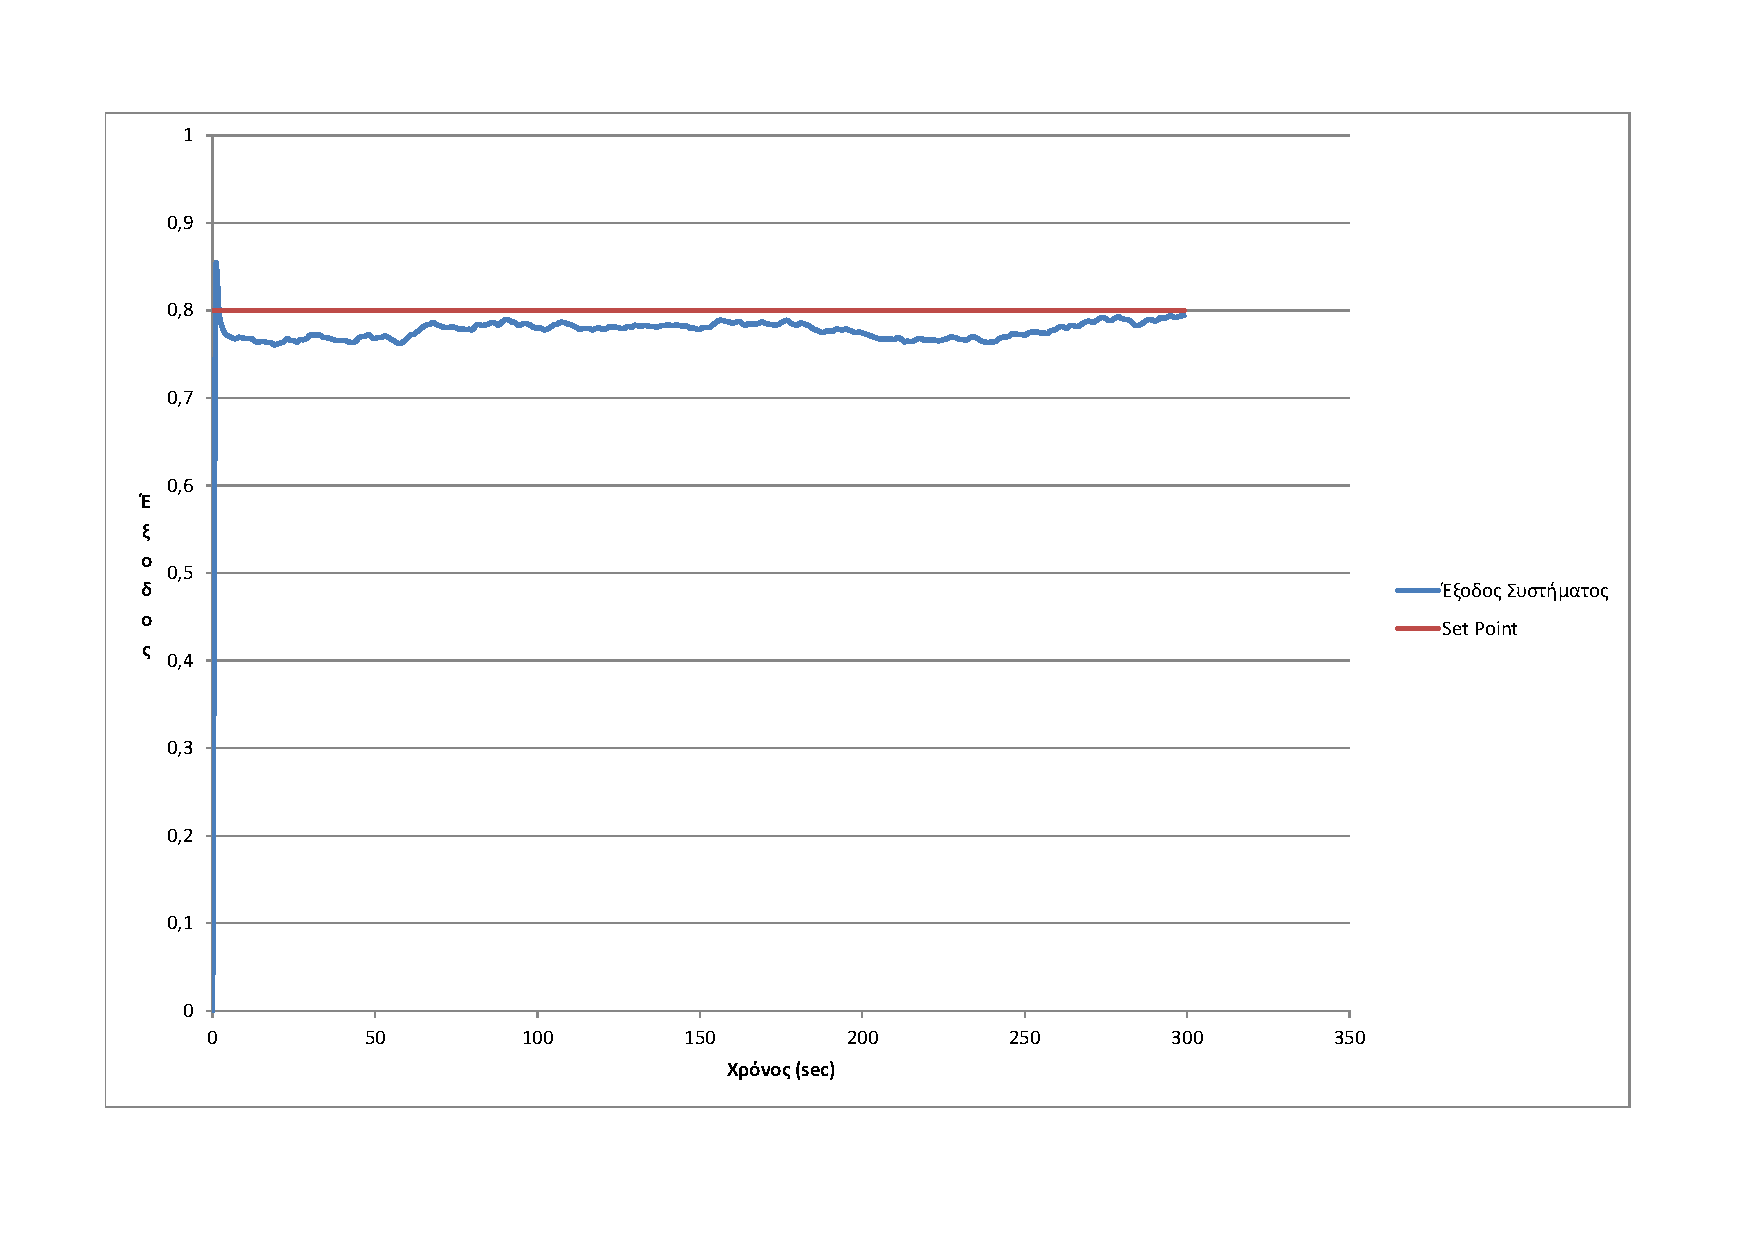
\includegraphics[width=0.9\textwidth]{siso_output_2_rewards.pdf}
    \caption{Προφίλ της εξόδου του συστήματος συναρτήσει του χρόνου με την χρήση της $\mathcal{R}$ συνάρτησης κέρδους}
    \label{fig:siso_output_2_rewards}
\end{figure}

\begin{figure}[H]
    \centering
    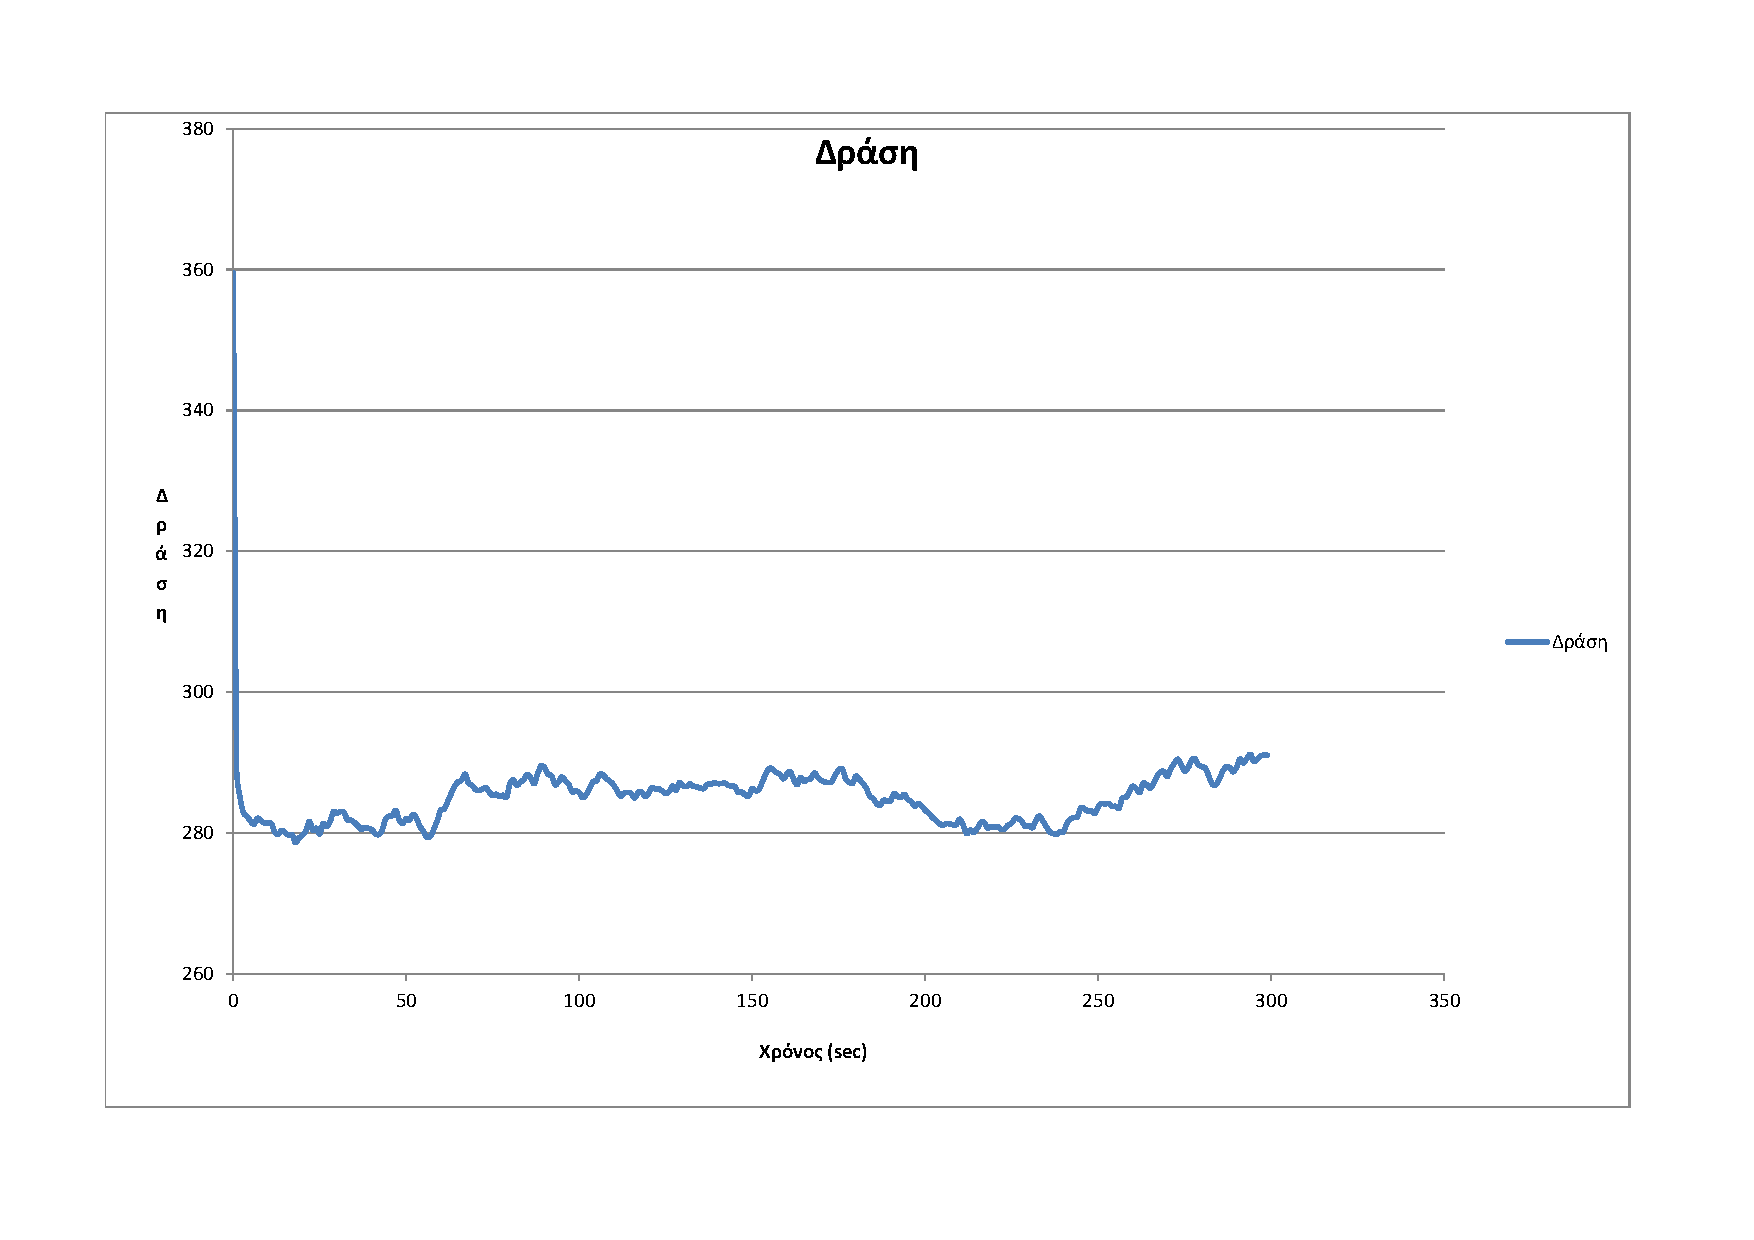
\includegraphics[width=0.9\textwidth]{action_output_2_reward.pdf}
    \caption{Προφίλ της δράσης του συστήματος συναρτήσει του χρόνου με την χρήση της $\mathcal{R}$ συνάρτησης κέρδους}
    \label{fig:action_output_2_rewards}
\end{figure}
 
Σε ό,τι αφορά την έξοδο του συστήματος παρατηρούμε ότι σε πολύ μικρό χρονικό διάστημα (σε μόλις ένα χρονικό βήμα) ο πράκτορας καταφέρνει και φτάνει στο set point, το ξεπερνά όμως κάνοντας μία μικρή υπέρβαση. Εν συνεχεία, πέφτει κάτω από το set point και συνεχίζει να το προσεγγίζει με ικανοποιητική ακρίβεια μέχρι το τέλος του επισοδείου οπού και φαίνεται να συγκλίνει σε αυτό. Το προφίλ της εξόδου είναι αρκετά θορυβώδες σε συμπεριφορά και αυτό οφείλεται στο προφίλ της δράσης του πράκτορα. Όπως φαίνεται στο παραπάνω διάγραμμα της δράσης, στα πολύ αρχικά στάδια του επισοδείου, ο πράκτορας δίνει μία αρκετά μεγάλου μεγέθους δράση, η οποία πέφτει με πολύ μεγάλο ρυθμό. Αυτή η αρχική δράση είναι υπεύθυνη για την μικρή υπέρβαση της εξόδου. Αφού η έξοδος υπερβεί το set point, ο πράκτορας ξέρει ότι πρέπει να επιφέρει ραγδαία μέιωση της δράσης για να πέσει κάτω από το set point και ύστερα να την προσαρμόσει κατάλληλα για να παραμείνει όσο το δυνατόν πιο κοντά σε αυτό. Και πράγματι μετά την αρχή του επισοδείου (όταν πλέον ο πράκτορας έχει πέσει κάτω από το set point) παρατηρούμε ότι το προφίλ της εξόδου και της δράσης είναι παρόμοια. Στις χρονικές στιγμές που η έξοδος φαίνεται να πλησιάζει το set point η δράση αυξάνεται, ενώ όταν η έξοδος φαίνεται να απομακρύνεται από το set point η δράση μειώνεται. Τελικά συμπεραίνουμε ότι η μόνιμη κατάσταση δεν επιτυγχάνεται κατά την διάρκεια του επισοδείου παρά μόνο ίσως στα τελικά στάδιά του όπου ο πράκτορας φαίνεται να έχει πλησιάσει πολύ κοντά στο set point.\\

Στην συνέχεια θα εξετάσουμε άλλα δύο διαφορετικά set points με την χρήση όμως αυτήν την φορά της συνάρτησης κέρδους $\mathcal{R}'$.

\begin{itemize}
\item Set Point = 0.9 και χρήση της $\mathcal{R}'$ συνάρτησης κέρδους
\end{itemize}
Στην περίπτωση αυτή η συνάρτηση κέρδους $\mathcal{R}'$ έχει μία βασική διαφορά σε σχέση με την $\mathcal{R}$. Η $\mathcal{R}'$ δίνει στον πράκτορα μία πολύ μεγάλη αμοιβή όταν καταφέρνει να είναι αρκετά ικανοποιητικά κοντά στο set point. Εδώ έχουμε θέσει ότι για να λάβει αυτή την μεγάλη αμοιβή θα πρέπει να είναι λιγότερο από 0.01 μακριά από το set point. Η λογική της συνάρτησης αυτής είναι ότι κατα πάσα πιθανότητα θα ωθήσει τον πράκτορα πιο κοντά στο set point και για περισσότερο χρόνο, αφού ο πρωταρχικός σκοπός του είναι να μαζέψει, μέχρι το τέλος του επισοδείου, το μεγαλύτερο δυνατό κέρδος. Τα αποτελέσματα είναι τα εξής:

\begin{figure}[H]
    \centering
    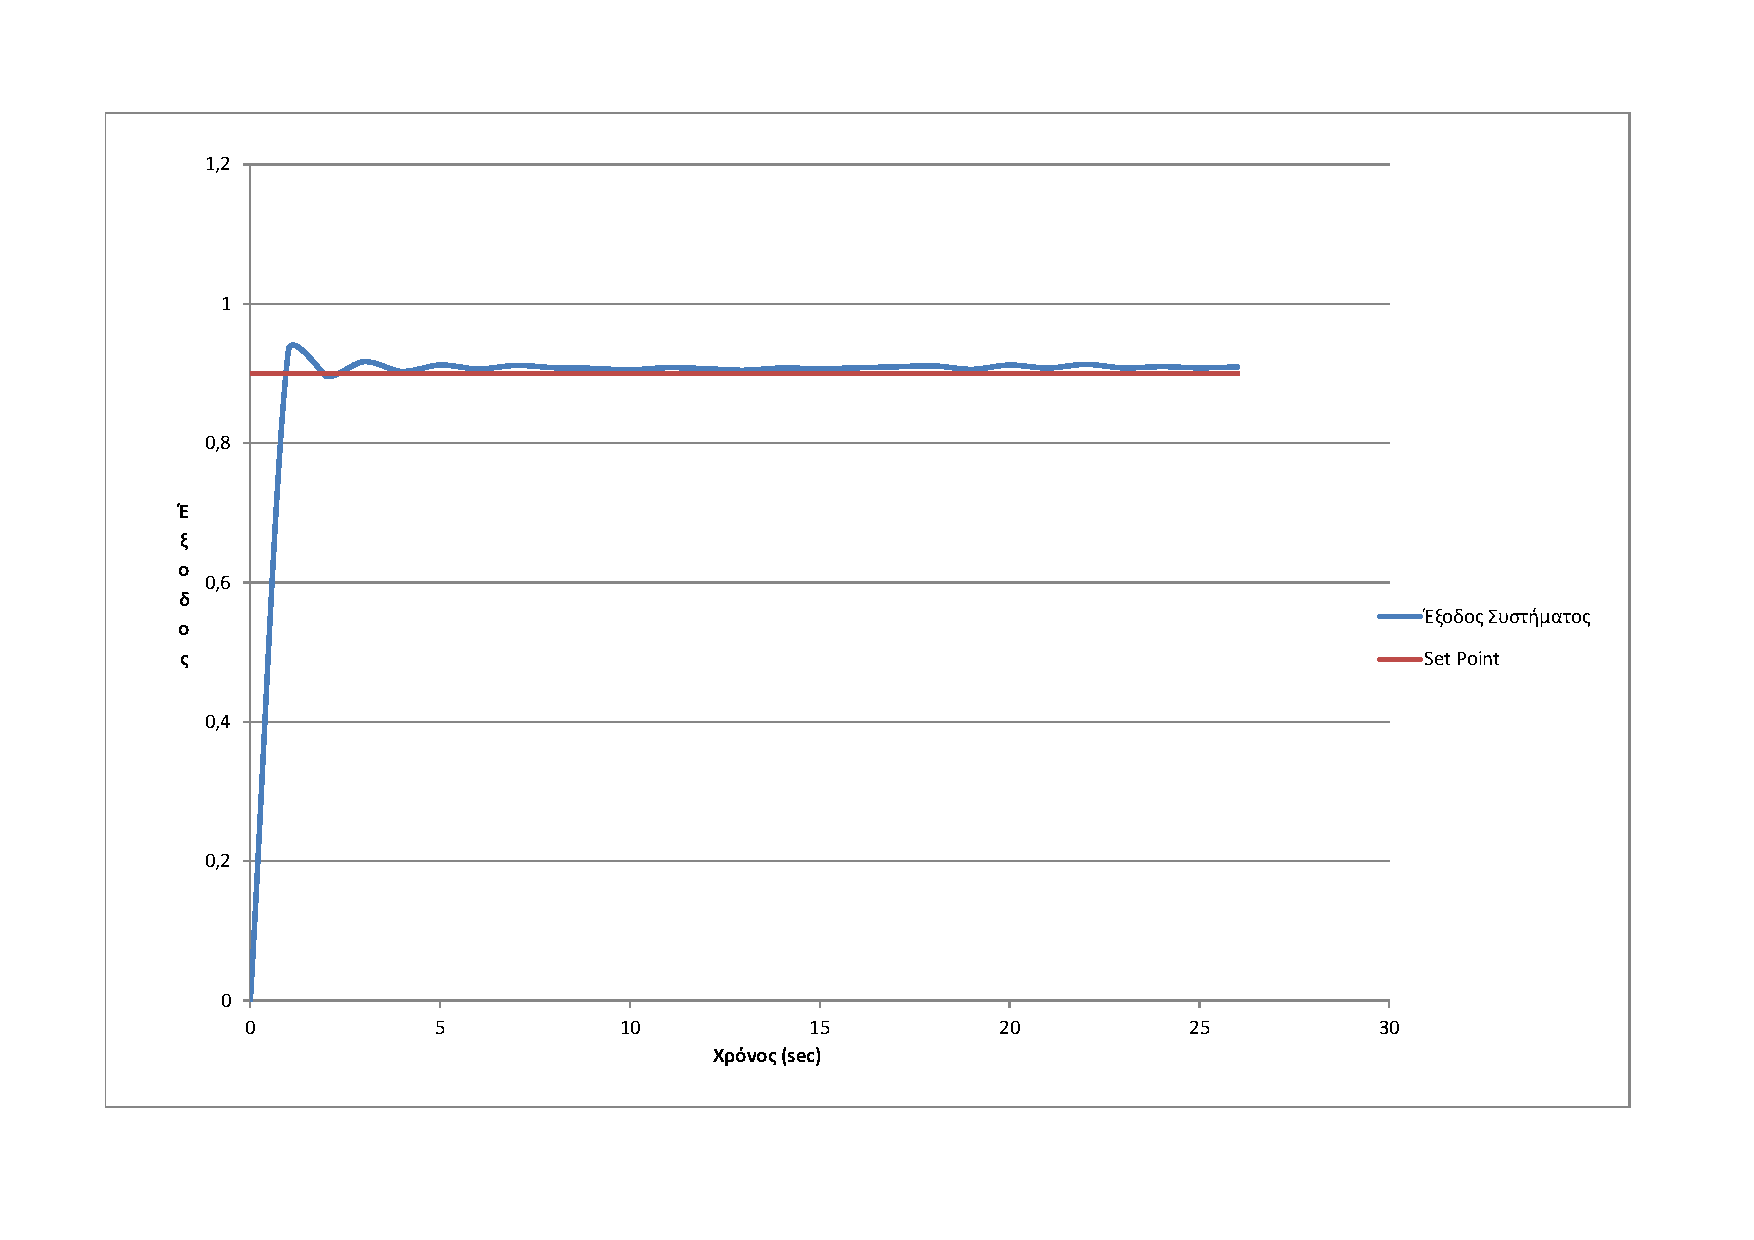
\includegraphics[width=0.9\textwidth]{siso_output_3_reward_09.pdf}
    \caption{Προφίλ της εξόδου του συστήματος συναρτήσει του χρόνου με την χρήση της $\mathcal{R}'$ συνάρτησης κέρδους}
    \label{fig:siso_output_3_rewards}
\end{figure}

\begin{figure}[H]
    \centering
    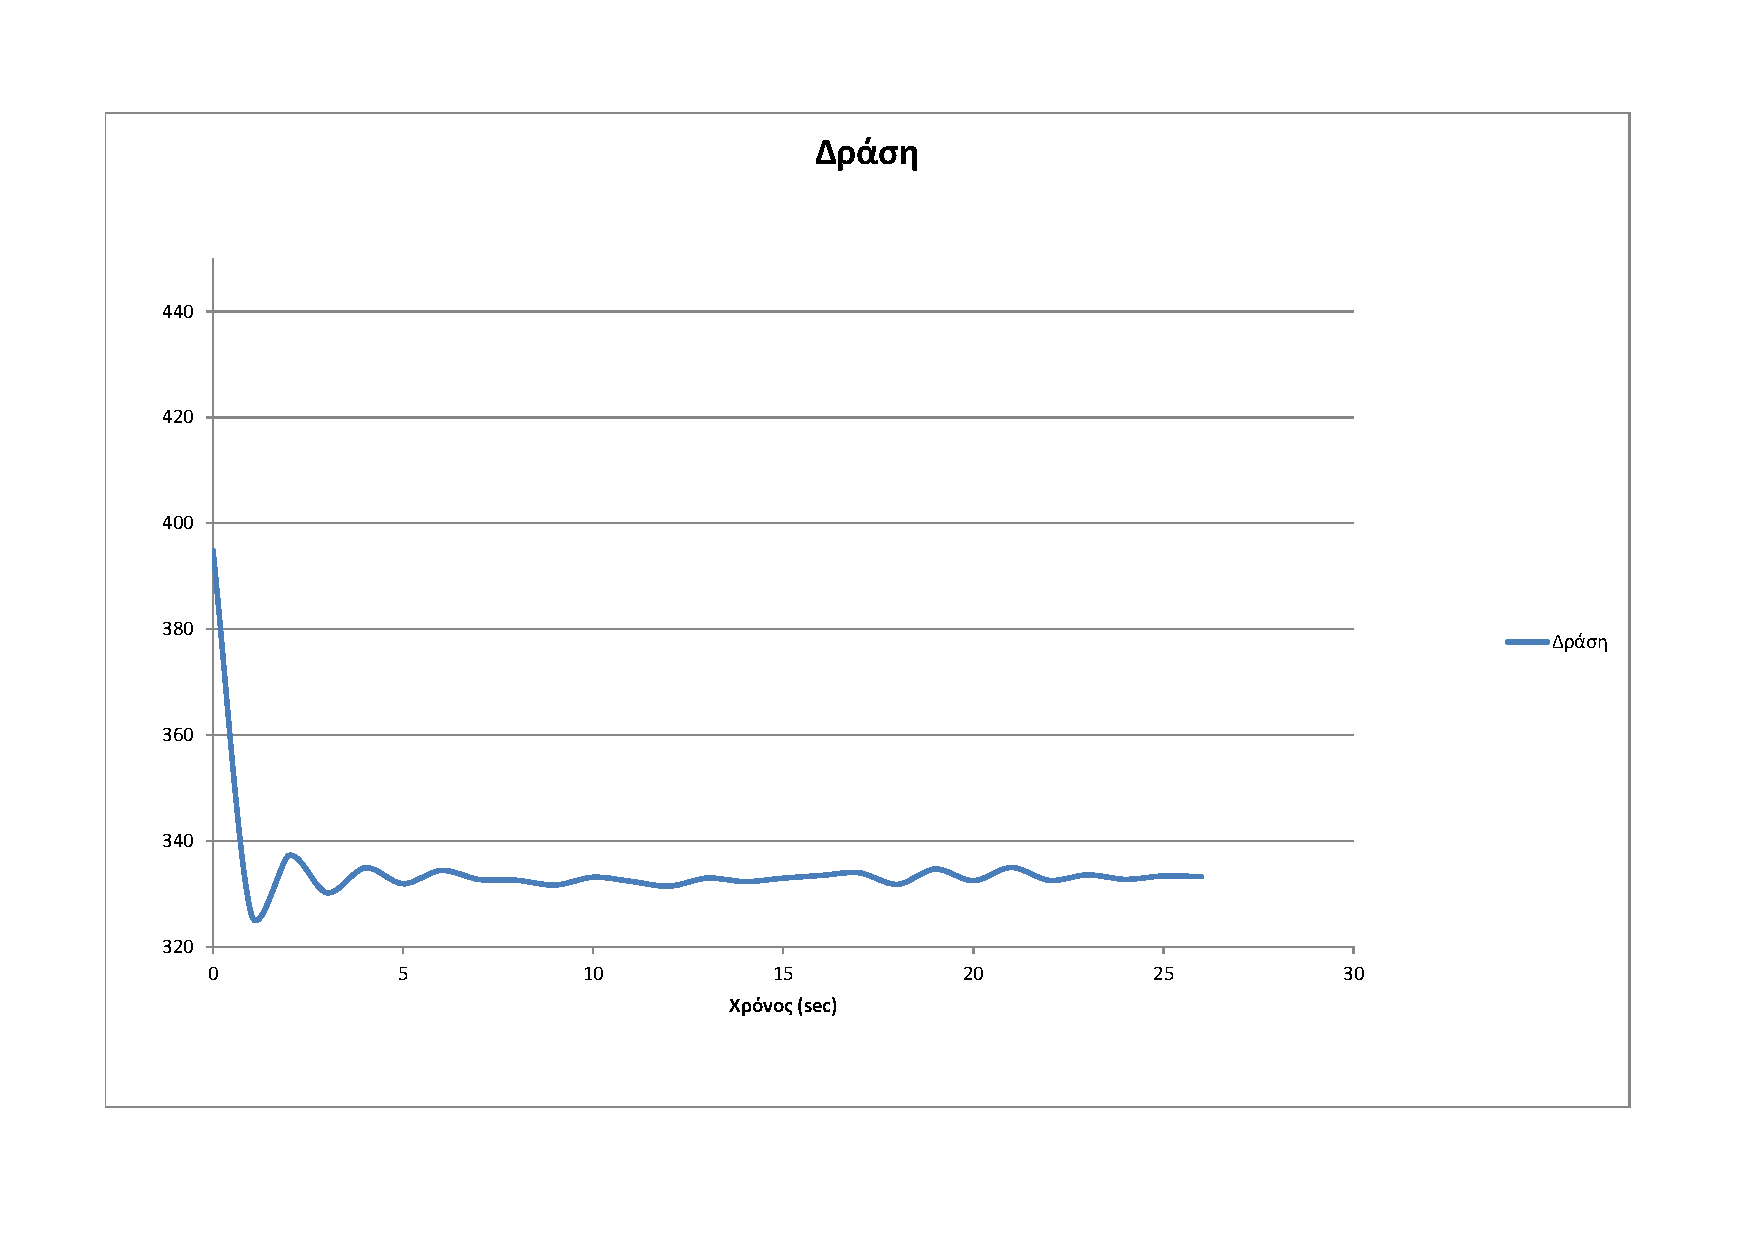
\includegraphics[width=0.9\textwidth]{siso_action_3_reward_09.pdf}
    \caption{Προφίλ της δράσης του συστήματος συναρτήσει του χρόνου με την χρήση της $\mathcal{R}'$ συνάρτησης κέρδους}
    \label{fig:siso_action_3_rewards}
\end{figure}

Όπως είναι προφανές τα αποτελέσματα σε αυτήν την περίπτωση είναι αρκετά διαφορετικά και μάλιστα πολύ καλύτερα. Στην αρχή του επισοδείου ο ρυθμιστής επιλέγει να δώσει μία αρκετά μεγάλη δράση η οποία, όπως και στην προηγούμενη περίπτωση, οδηγεί σε μία μικρή υπέρβαση της εξόδου (περίπου της ίδιας τάξεως). Στην συνέχεια η δράση πέφτει με αρκετά μικρότερη κλίση, έτσι ώστε ο πράκτορας να πλησιάσει το set point. Από εκεί και πέρα παρατηρούμε ένα σχετικά ομαλό προφίλ δράσης το οποίο φυσικά συνεπάγεται ένα πολύ ομαλό προφίλ εξόδου. Πιο συγκεκριμένα η έξοδος του συστήματος φαίνεται να ταλαντεύεται πολύ κοντά γύρω από το set point μέχρι το όγδοο χρονικό βήμα και μετά πρακτικά συγκλίνει σε αυτό. Η νέα επιβαλλόμενη συνάρτηση κέρδους όντως ωθεί τον πράκτορα πολύ κοντά στο set point και διατηρεί πολύ κοντινές αποστάσεις γύρω από αυτό. Με αυτόν τον τρόπο ο πράκτορας μπορεί, μέχρι το τέλος του επισοδείου, να μαζέψει αρκετά μεγάλο κέρδος. Η μόνιμη κατάσταση φαίνεται να επιτυγχάνεται με μεγάλη ακρίβεια μετά το δέκατο χρονικό βήμα.\\

Ως τελευταία εφαρμογή της μεθοδολογίας DDPG σε γραμμικό σύστημα δοκιμάζουμε την ίδια συνάρτηση κέρδους, $\mathcal{R}'$ σε ένα διαφορετικό set point.\\

\begin{itemize}
\item Set Point = 0.5 και χρήση της $\mathcal{R}'$ συνάρτησης κέρδους
\end{itemize}
Η προσομοίωση αυτή γίνεται πιο πολύ για να δοκιμασθεί η ευρωστία της συνάρτηση κέρδους $\mathcal{R}'$, δηλαδή για να δούμε αν μπορεί να δώσει τα ίδια επιτυχημένα αποτελέσματα για ένα διαφορετικό set point. Όλες οι υπόλοιπες παράμετροι της προσομοίωσης παραμένουν ίδιες. Παίρνουμε τα εξής αποτελέσματα:

\begin{figure}[H]
    \centering
    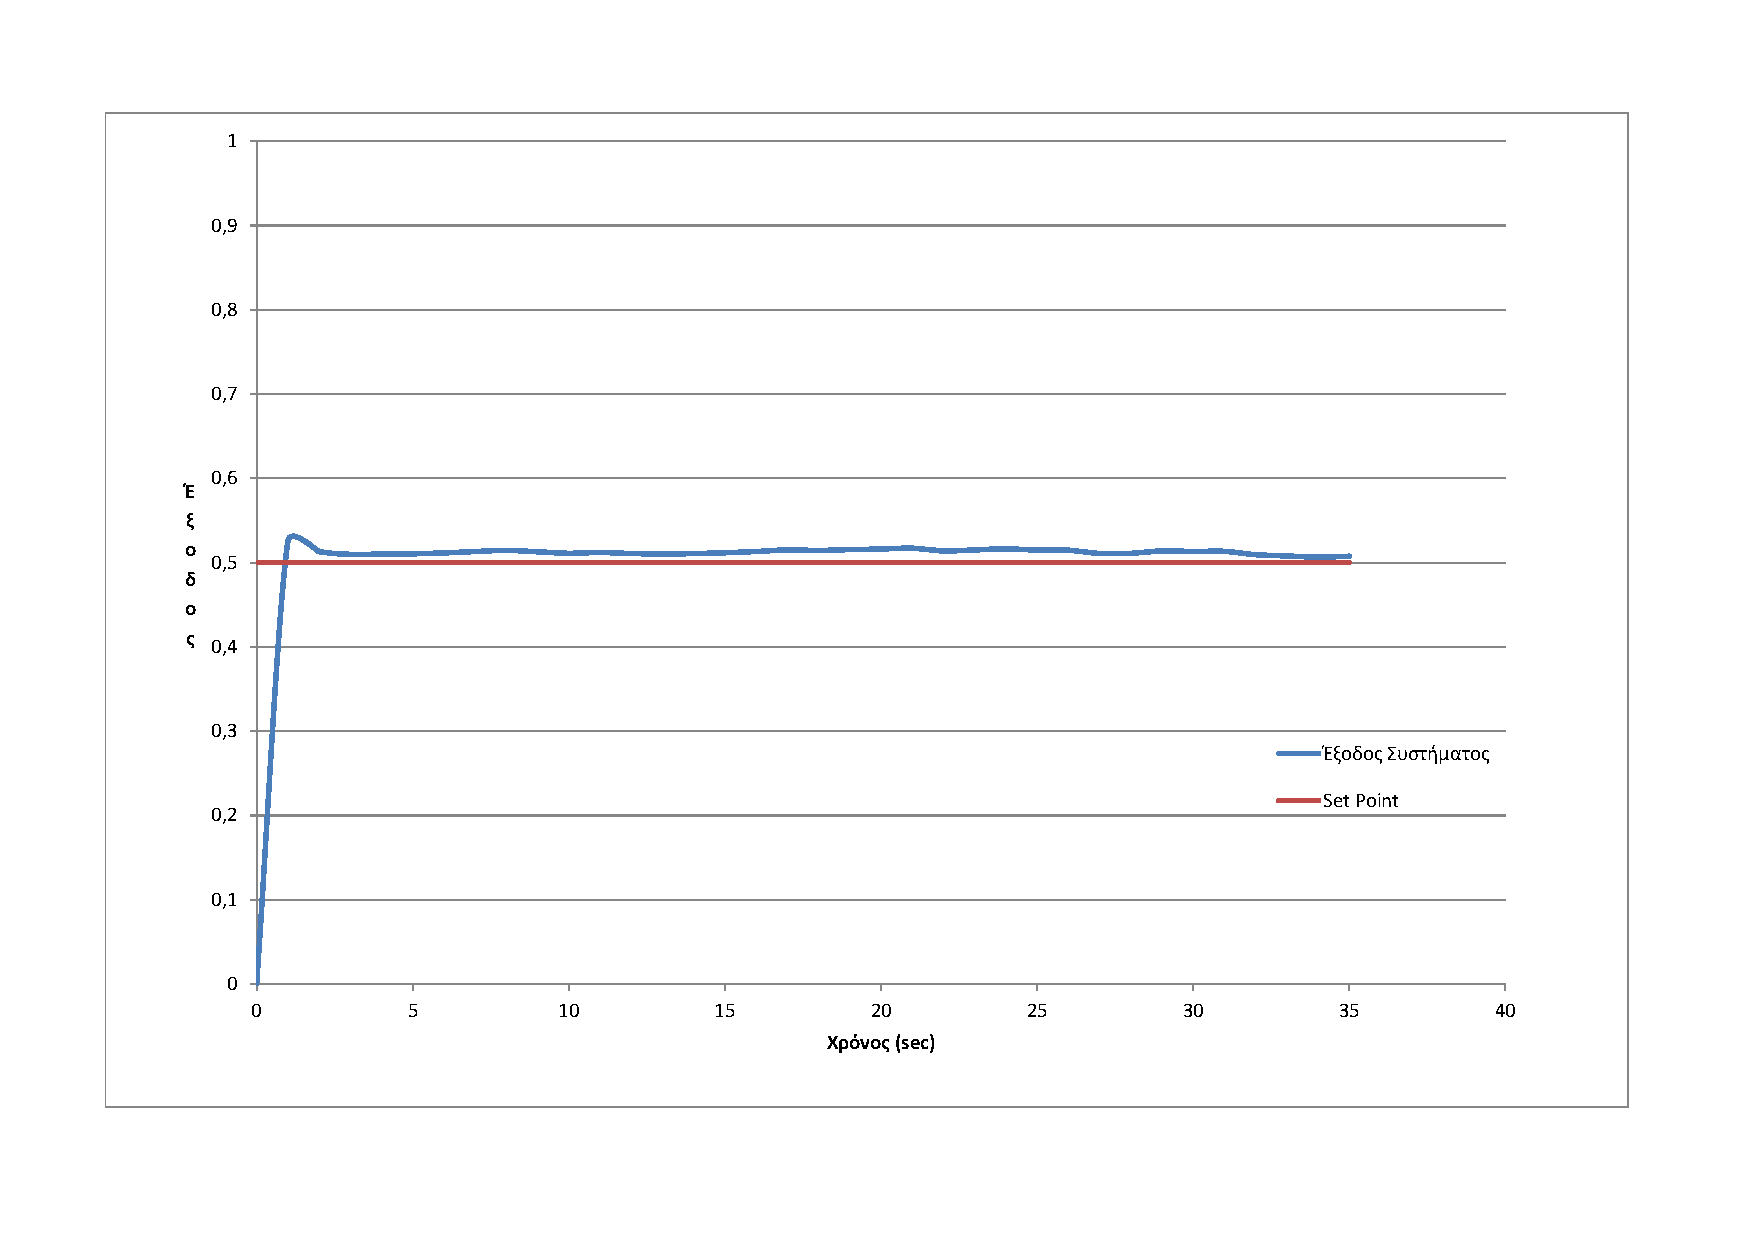
\includegraphics[width=0.8\textwidth]{siso_output_3_reward_05.pdf}
    \caption{Προφίλ της εξόδου του συστήματος συναρτήσει του χρόνου με την χρήση της $\mathcal{R}'$ συνάρτησης κέρδους}
    \label{fig:siso_output_3_rewards_05}
\end{figure}

\begin{figure}[H]
    \centering
    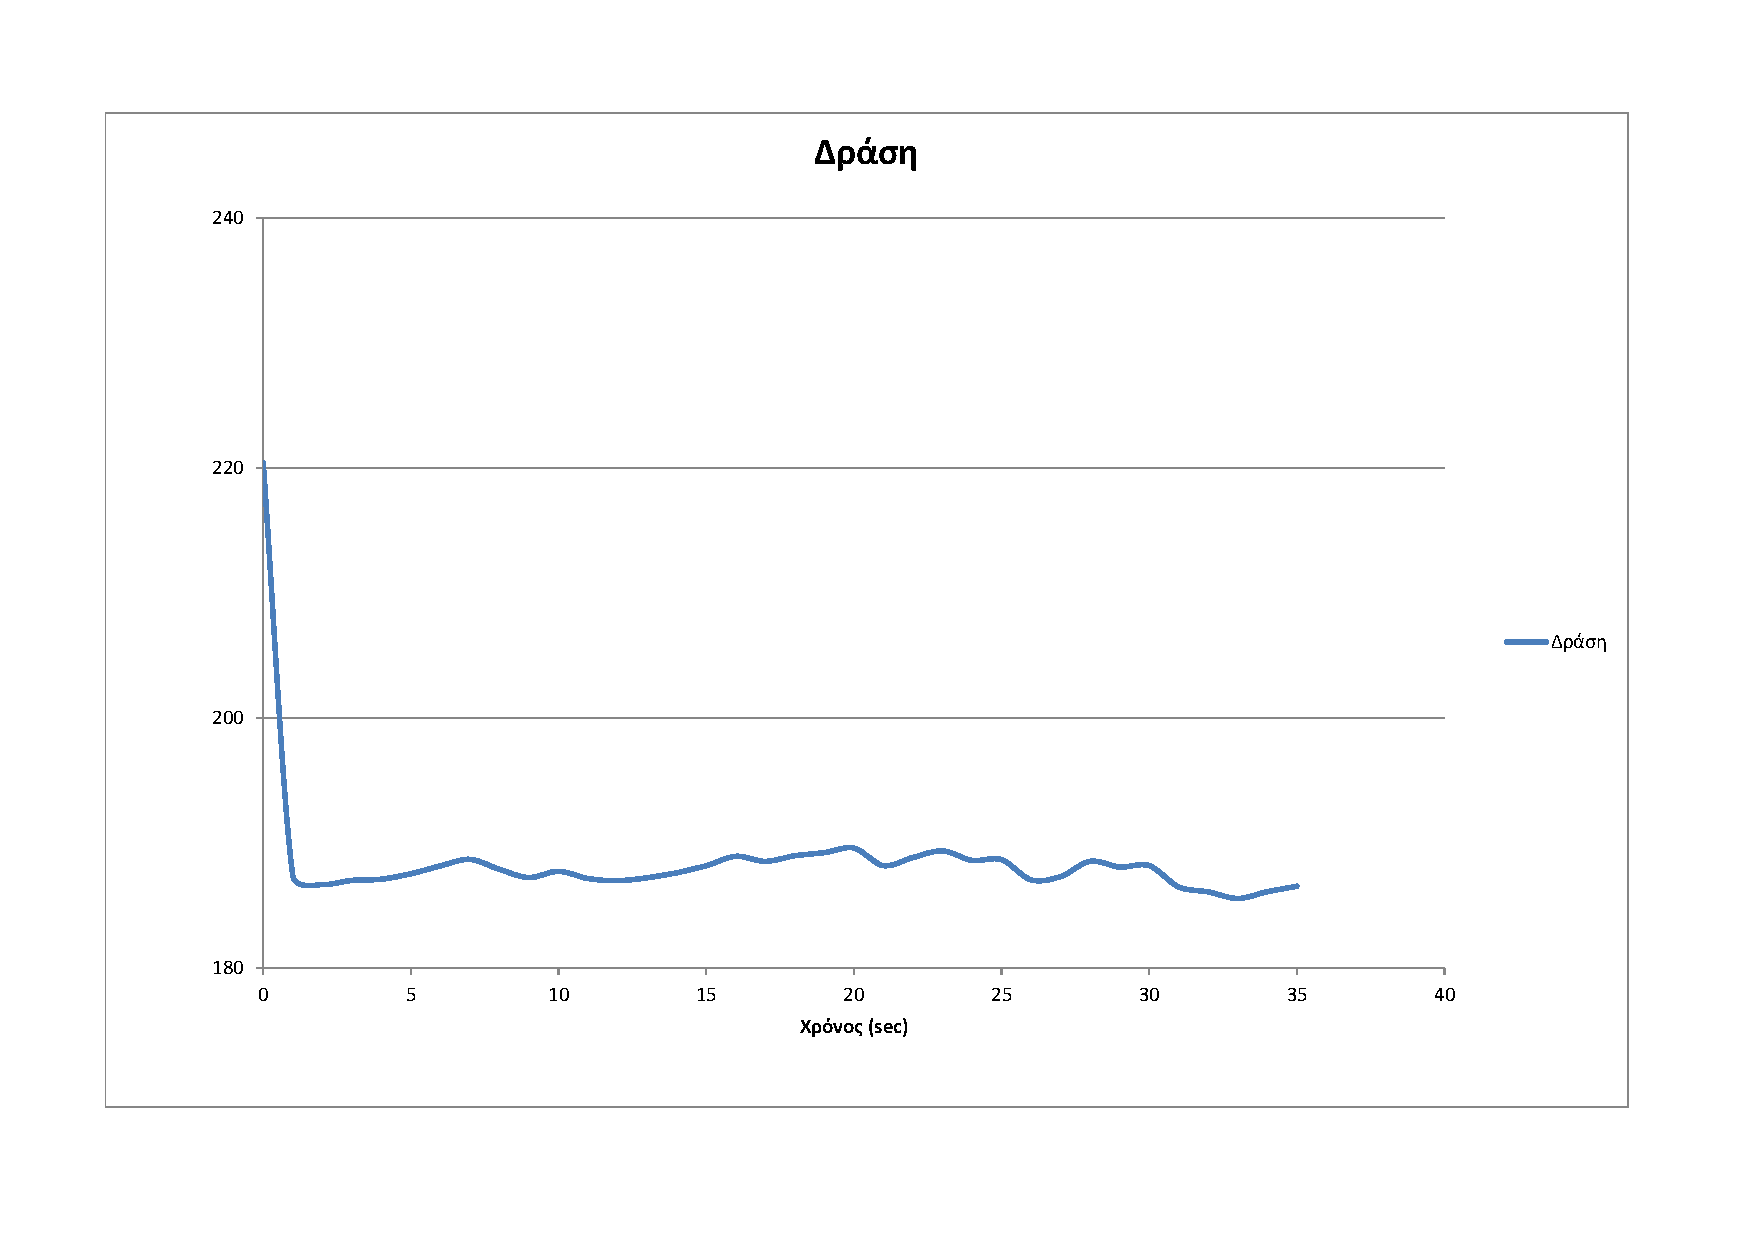
\includegraphics[width=0.8\textwidth]{siso_action_3_reward_05.pdf}
    \caption{Προφίλ της δράσης του συστήματος συναρτήσει του χρόνου με την χρήση της $\mathcal{R}'$ συνάρτησης κέρδους}
    \label{fig:siso_action_3_rewards_05}
\end{figure}

Όπως φαίνεται η συμπεριφορά του συστήματος υπό την επίδραση της ίδιας συνάρτησης κέρδους είναι πολύ παρόμοια. Υπάρχει μία μικρή υπέρβαση στα αρχικά στάδια του επισοδείου και έπειτα ο πράκτορας πλησιάζει το set point και παραμένει πολύ κοντά σε αυτό, επιτυγχάνοντας έτσι μόνιμη κατάσταση. Το προφίλ της δράσης είναι προφανώς πολύ παρόμοιο με αυτό που αντιστοιχούσε στο set point 0.9 και είναι αυτό ουσιασικά που καθορίζει και την εξίσου παρόμοια με πριν συμπεριφορά της εξόδου. Συμπεραίνουμε λοιπόν ότι η προτεινόμενη συνάρτηση κέρδους $\mathcal{R}'$ είναι καταλληλότερη για την εκπαίδευση του εν λόγω συστήματος.\\

Στην συνέχεια θα εξετάσουμε κατά πόσο η μεθοδολογία DDPG μπορεί να αντιμετωπίσει ένα αρκετά πιο δύσκολο πρόβλημα ρύθμισης.

\subsection{Εφαρμογή της μεθοδολογίας DDPG σε μη-γραμμικό μοντέλο δύο εισόδων και δύο εξόδων}
Το επόμενο βήμα είναι η δοκιμασία της προτεινόμενης μεθοδολογίας ρύθμισης σε ένα μη-γραμμικό μοντέλο, το οποίο δανειστήκαμε από την βιβλιογραφία \cite{cstr}. Το μοντέλο αυτό δίνεται από τις παρακάτω εξισώσεις:
\begin{equation}
\begin{split}
\frac{dC_{A}}{dt} = \frac{F}{V}(C_{A,in} - C_{A}) - 2k_{0} \exp\left(-\frac{E}{RT}\right)C_{A}^2 \\
\frac{dT}{dt} = \frac{F}{V}(T_{in} - T) - 2\frac{(-ΔΗ_{R})}{ρc_{p}}k_{0} \exp\left(-\frac{E}{RT}\right)C_{A}^2 - \frac{UA}{Vρc_{p}}(T - T_{j})
\end{split}
\end{equation}

Πρόκειται δηλαδή για τις εξισώσεις λειτουργίας (ισοζύγιο μάζας και ενέργειας) ενός \textit{μη-ισοθερμοκρασιακού αντιδραστήρα CSTR} στον οποίο λαμβάνει χώρα η εξώθερμη αντίδραση $Α \rightarrow B$ στην υγρή φάση. $Ε$ είναι η ενέργεια ενεργοποίησης της αντίδρασης, $k_{0}$ η σταθερά Arrhenius, $R$ η παγκόσμια σταθερά των αερίων, $ΔΗ_{R}$ ο θερμοτονισμός της αντίδρασης, $\rho$ η πυκνότητα της υγρής φάσης που εισέρχεται στον αντιδραστήρα, $V$ o όγκος του αντιδραστήρα, $c_{p}$ η θερμοχωρητικότητα του ψυκτικού μέσου, $U$ ο συντελεστής μεταφοράς θερμότητας του ψυκτικού και $Α$ η επιφάνεια εναλλαγής θερμότητας.\\

Στο πρόβλημα αυτό θεωρούμε ως μεταβλητές εισόδου την ροή εισόδου στον αντιδραστήρα, $F$ και την θερμοκρασία του ψυκτικού μέσου, $Τ_{j}$, και ως μεταβλητές εξόδου την συγκέντρωση του αντιδρώντος Α, $C_{A}$ και την θερμοκρασία του αντιδραστήρα $Τ$. Στόχος του ρυθμιστή δηλαδή είναι να βρει το χρονικό προφίλ της ροής εισόδου και της θερμοκρασίας του ψυκτικού μέσου ώστε το σύστημα μας να φτάσει στην επιθυμητή κατάσταση $(C_{A,set},T_{set})$. Στην περίπτωση αυτή το ψυκτικό μέσο είναι απαραίτητο γιατί η αντίδραση που λαμβάνει χώρα είναι ισχυρά εξώθερμη οπότε η θερμοκρασία του αντιδραστήρα μπορεί να ανέβει σε πολύ υψηλά επίπεδα χωρίς την βοήθεια ψυκτικού. Οι τιμές των διαφόρων παραμέτρων του συστήματος δίνονται στον παρακάτω πίνακα.\\
\begin{table}[H]
\centering
\begin{tabular}{ |p{3cm}|p{3cm}|p{3cm}| }
\hline
Παράμετρος Διεργασίας& Αριθμητική Τιμή& Μονάδα Μέτρησης \\
\hline
V  & 100 &[lt] \\
UA & 20000   & [J/min K] \\
ρ  &1000 & [g/lt] \\

$c_{p}$   &4.2 & [J/g K] \\
$-(ΔΗ_{R})$ & 596619 & [J/mol] \\
$k_{0}$ & 6.85E+11 & [lt/min mol]   \\
E & 76534.704 & [J/mol] \\
R & 8.314 & [J/mol K]\\
$T_{in}$ & 275 & [K]\\
$C_{A,in}$ & 1 & [mol/lt]\\
\hline
\end{tabular}
\caption{Πίνακας παραμέτρων της διεργασίας}
\label{table:10}
\end{table}

Θα πρέπει τώρα και πάλι να μετφράσουμε τα δεδομένα μας σε γλώσσα ενισχυτικής μάθησης. Ως κατάσταση του συστήματος θεωρούμε το τετράνυσμα:
\begin{align*}
\textbf{s}(t) = (C_{A}(t), C_{A_{set}}, T(t), T_{set})
\end{align*}

Ο λόγος που η κατάσταση ορίζεται με αυτόν τον τρόπο είναι παρόμοιος με το σύστημα μίας εξόδου και εισόδου που μελετήσαμε. Ο ρυθμιστής προκειμένου να λάβει μία δράση θα πρέπει να ξέρει τόσο την συγκέντρωση του Α όσο και την θερμοκρασία του αντιδραστήρα αλλά και τις επιθυμητές προδιαγραφές μας, δηλαδή τα set points. Στο συγκεκριμένο πρόβλημα προσδιορίζουμε την  κατάσταση του συστήματος (δηλαδή υπολογίζουμε τις τιμές $C_{A}(t)$ και $T(t)$ σε κάθε χρονικό βήμα ενός επισοδείου λύνοντας το παραπάνω σύστημα μη-γραμμικών διαφορικών εξισώσεων με την ρουτίνα odeint της βιβλιοθήκης scipy της Python\\

Η συνάρτηση πολιτικής μας τώρα είναι η διανυσματική συνάρτηση:
\begin{align*}
\textbf{\mu}(t) = (F(t), T_{j}(t))
\end{align*}

και ομοίως με πριν ορίζουμε ως δράση την διανυσματική συνάρτηση:
\begin{align*}
 \textbf{\alpha}(t) = \textbf{\mu}(t) + \mathcal{N}(t) = (F(t) + \mathcal{N}_{0}(t), T_{j}(t) + \mathcal{N}_{1}(t))
\end{align*}

όπου και πάλι $\mathcal{N}(t) = (\mathcal{N}_{1}(t), \mathcal{N}_{2}(t))$ ο θόρυβος κατά Ornstein-Uhlenbeck. Εφόσον στο πρόβλημά μας τώρα ο χώρος των δράσεων είναι δύο διαστάσεων χρειαζόμαστε δύο τυχαίους περιπάτους προς εξερεύνηση του χώρου, έναν για κάθε δράση. Ομοίως με πριν, η δράση κάνει τον πράκτορα να μεταβεί από την τρέχουσα κατάσταση στην επόμενη, την οποία θα συμβολίσουμε ως:
\begin{align*}
\textbf{s}'(t) = (C_{A}(t+1), C_{A_{set}}, T(t+1), T_{set})
\end{align*}

Η συνάρτηση κέρδους, $r(s, \alpha, s')$, ορίζεται τώρα ως:
\[ 
\ r(s, \alpha, s') = \left\{
\begin{array}{ll}
      1 & , \abs{C_{A}(t+1) - C_{A_{set}}} < \abs{C_{A}(t) - C_{A_{set}}} και \abs{T(t+1) - T_{set}} < \abs{ T(t) - T_{set}} \\
      200 & , \abs{C_{A_{t+1}} - C_{A_{set}}} < 0.003 \hspace{0.3cm} και \hspace{0.3cm} \abs{ T(t+1), T_{set}} < 1 \\
	-100 & , T_{j}(t) + \mathcal{N}_{1}(t) > 300\\
	-10, αλλιως
\end{array} 
\right. 
\]

Η λογική της παραπάνω συνάρτησης κέρδους είναι η εξής: Δίνουμε στον πράκτορα μία μικρή αμοιβή (+1) κάθε φορά που τόσο η συγκέντρωση του Α όσο και η θερμοκρασία του αντιδραστήρα πλησιάζουν κατ'απόλυτη τιμή τα επιθυμητά set points. Δίνουμε μία πολύ μεγάλη θετική αμοιβή (+200) όταν το σύστημά μας είναι ικανοποιητικά κοντά στα set points, έτσι ώστε να ωθήσουμε τον πράκτορα να παραμείνει κοντά τους για μεγαλύτερο χρονικό διάστημα. Επίσης δίνουμε στον πράκτορα μεγάλη αρνητική αμοιβή (-100) κάθε φορά που η δράση της θερμοκρασίας του ψυκτικού είναι πάνω από 300K. Αυτό γίνεται έτσι ώστε να αποφευχθούν για όσο το δυνατόν πιο πολλά χρονικά βήματα θερμοκρασίες ψυκτικού που είναι πάνω από 300K. Προσπαθούμε δηλαδή να περιορίσουμε την θερμοκρασία του ψυκτικού σε όσο στενότερα όρια γίνεται μέσω της συνάρτησης κέρδους. Τέλος αν καμία από αυτές τις συνθήκες δεν πληρείται δίνουμε στον πράκτορα μία αρνητική αμοιβή (-10). Ο λόγος που δίνουμε αρνητική αμοιβή μεγαλύτερη κατ'απόλυτη τιμή από +1 (η αμοιβή του πρώτου κλάδου της συνάρτησης) είναι για να ωθήσουμε τον πράκτορα να πλησιάσει πιο γρήγορα και πιο αποδοτικά τα set points, εφόσον ο στόχος του είναι να μαζέψει κατά το δυνατόν μεγαλύτερο κέρδος στο τέλος ενός επισοδείου.\\

Τώρα θα παρουσιάσουμε τις παραμέτρους της μεθοδολογίας που χρησιμοποιήθηκαν για την προσομοίωση:\\

Τα νευρωνικά δίκτυα του δράστη, του κριτή αλλά και τα αντίστοιχα δίκτυα-στόχοι έχουν το καθένα από δύο κρυφά στρώματα. Το πρώτο κρυφό στρώμα έχει 450 νευρώνες και το δεύτερο έχει 400 νευρώνες. Όλες οι συναρτήσεις ενεργοποίησης επιλέχθηκαν και εδώ ως τύπου ReLU. Ο ρυθμός εκμάθησης για όλα τα δίκτυα είναι ίσος με $5 \cdot 10^{-4}$ και, ομοίως με πρίν $\tau = 10^{-3}$. Αυτήν την φορά δεν έχουμε επιβάλλει κάποιου είδους κανονικοποίησης κόστους. Ο παράγοντας προεξόφλησης είναι ίσος με 0.99. Χωρητικότητα μνήμης αναπαραγωγής ίση με $10^{4}$, ίση και με τον χρόνο προθέρμανσης. Το μέγεθος των παρτίδων τώρα είναι ίσο με 128. Τα κρυφά στρώματα είναι κανονικοποιημένα. Σαν βελτιστοποιητής χρησιμοποιήθηκε και πάλι ο GradientDescentOptimizer. Στο σημείο αυτό κρίνεται σκόπιμο να αναφερθεί ότι στις αρχικές προσομοιώσεις του εν λόγω συστήματος είχε χρησιμοποιηθεί ο Adam Optimizer \cite{adam} του Tensorflow. Παρόλα αυτά ακόμη και μετά από αρκετές ώρες μέσα στην προσομοίωσης ο αλγόριθμος δεν κατάφερε να συγκλίνει. Για τον σκοπό αυτό δοκιμάσθηκε ο GradientDescentOptimizer και τα αποτελέσματα που θα παρουσιασθούν λήφθηκαν μετά από περίπου μίαμιση ώρα μέσα στην προσομοίωση.\\

Και εδώ ένα επισόδειο διαρκεί για 300 χρονικά βήματα. Ομοίως με την προηγούμενη περίπτωση ένα επισόδειο τελειώνει όταν:
\begin{itemize}
  \item Το επισόδειο έχει ολοκληρωθεί, δηλαδή ο αλγόριθμος έχει τρέξει για 300 χρονικά βήματα
  \item Ο ρυθμιστής έχει καταφέρει να εντοπίσει το set point και έχει καταφέρει να παραμείνει ικανοποιητικά κοντά σε αυτό για 5 χρονικά βήματα, δηλαδή ικανοποιούνται οι ανισώσεις $\abs{C_{A_{t+1}} - C_{A_{set}}} < 0.003$ και $\abs{T(t+1), T_{set}} < 1$ για πέντε χρονικά βήματα
\end{itemize}

Και στην περίπτωση αυτή στην αρχή του κάθε επισοδείου θα πρέπει να επαναφέρουμε το σύστημα στην αρχική του κατάσταση , δηλαδή σε συγκέντρωση Α ίση με την συγκέντρωση εισόδου και θερμοκρασία ίση με την θερμοκρασία εισόδου.\\

Στις παραπάνω παραμέτρους δεν έχουν συμπεριληφθεί οι παράμετροι του θορύβου Ornstein-Uhlenbeck, δηλαδή του τυχαίου περιπάτου. Ο λόγος είναι επειδή στο συγκεκριμένο σύστημα έχουμε εξετάσει πώς ο θόρυβος αυτός επηρεάζει την προσομοίωση και την συμπεριφορά του συστήματος. Έχουν γίνει δηλαδή δύο προσομοιώσεις -για το ίδιο set point- μία χωρίς θόρυβο και μία με θόρυβο, οι παράμετροι των οποίων θα αναφερθούν παρακάτω.\\

Το διάνυσμα του set point που θα θέσουμε για τις προσομοιώσεις που θα ακολουθήσουν είναι το εξής
\begin{align*}
s_{set} = (C_{A_{set}}, T_{set}) = (0.07, 375)
\end{align*}
Τα set points αυτά δεν επιλέχθηκαν τυχαία. Συγκεκριμένα, το σημείο $s_{eq} = (C_{A_{eq}}, T_{eq}) = (0.0754, 376.3)$ αποτελεί \textit{ευσταθές σημείο ισορροπίας} του δυναμικού συστήματος (9.2.1). Πράγματι αν στο σύστημα αυτό μηδενίσουμε τις παραγώγους, αντικαταστήσουμε τις παραμέτρους του πίνακα 6 αλλά και τις εξής τιμές της ροής εισόδου και της θερμοκρασίας του ψυκτικού
\begin{align*}
F_{eq} = 20 \frac{lt}{min}\\
T_{j, eq} = 250 K
\end{align*}
και λύσουμε το $2 \times 2$ σύστημα μη-γραμμικών εξισώσεων που προκύπτει τότε θα πάρουμε ως λύση το σημείο $s_{eq}$. Ο τρόπος με τον οποίο αποφανθήκαμε ότι το παραπάνω σημείο ισορροπίας είναι ευσταθές ήταν με την μέθοδο της  \textit{απειροστής μεταβολής των παραμέτρων}.  Η μέθοδος αυτή συνίσταται στην εισαγωγή μίας μικρής διαταραχής στις παραπάνω μεταβλητές ισορροπίας $F_{eq}$ και $T_{j, eq}$
\begin{align*}
F_{eq, pert} = F_{eq} + dF\\
T_{j,eq,pert} = T_{j, eq} + dT_{j}\\
\end{align*}
όπου οι μικρές αυτές διαταραχές είναι της τάξεως του $10^{-2}$. Αν επιβάλλοντας αυτές τις διαταραχές παρατηρήσουμε ότι το σύστημα δίνει μία τελείως διαφορετική λύση, πολύ μακριά από το σημείο ισορροπίας, τότε το σημείο ισορροπίας χαρακτηρίζεται ως \textit{ασταθές}. Αν αντιθέτως η λύση είναι κοντά στο σημείο ισορροπίας τότε χαρακτηρίζεται ως \textit{ευσταθές}. Με την παραπάνω μέθοδο συμπεραίνουμε ότι το εν λόγω σημείο ισορροπίας $s_{eq}$ είναι ευσταθές.\\

Συνεπώς το επιθυμητό set point της προσομοίωσης βρίσκεται σε μία γειτονιά του ευσταθούς σημείου ισορροπίας. \\


Ξεκινάμε τώρα με την παρουσίαση των αποτελεσμάτων:\\
\begin{itemize}
\item $C_{A_{set}} = 0.07$ , $Τ_{set} = 375$ με την χρήση θορύβου κατά Ornstein-Uhlenbeck
\end{itemize}
Οι παράμετροι του θορύβου που χρησιμοποιήθηκαν είναι $\mu = 0, \theta = 0.15, \sigma = 0.2$. Τα αποτελέσματα φαίνονται στα παρακάτω διαγράμματα:
\begin{figure}[H]
    \centering
    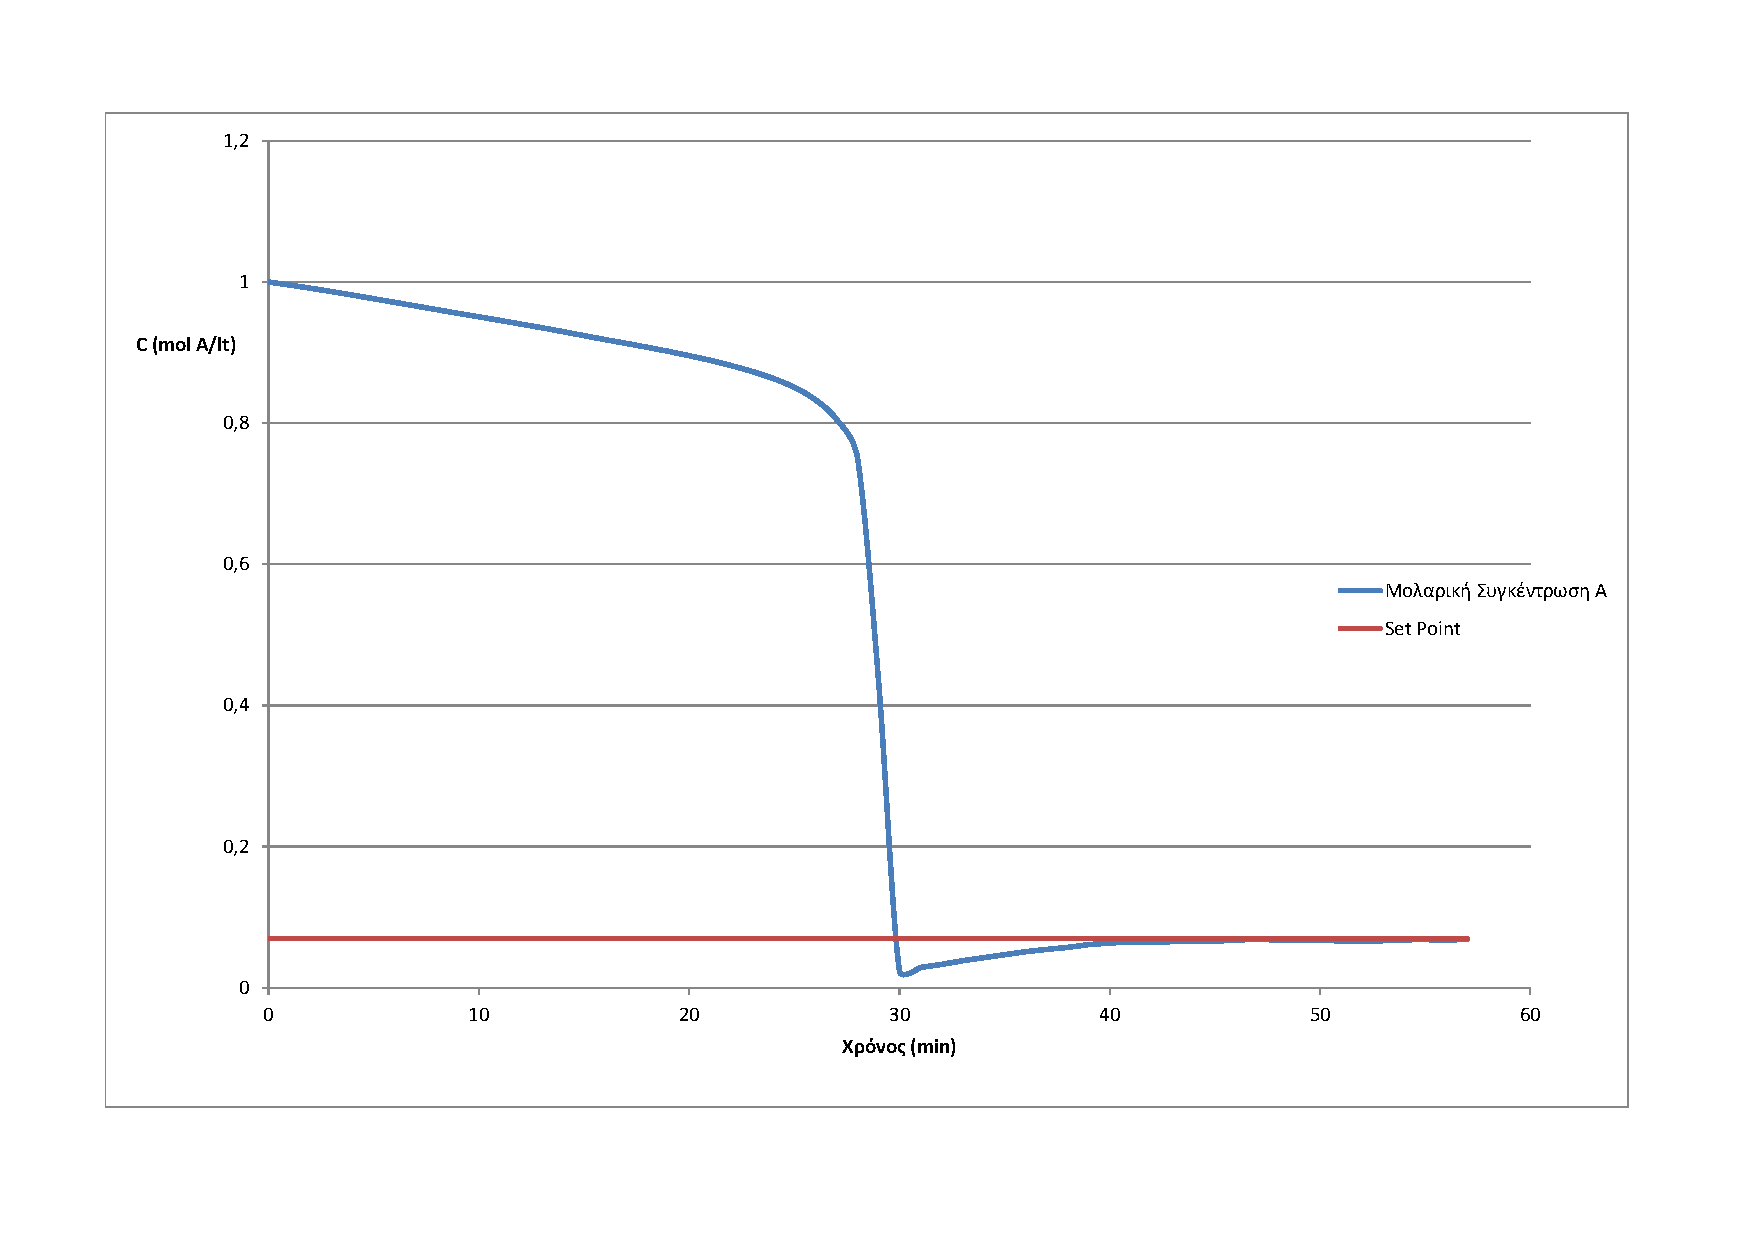
\includegraphics[width=0.8\textwidth]{noise_ca.pdf}
    \caption{Προφίλ της συγκέντρωσης του Α συναρτήσει του χρόνου με την χρήση θορύβου}
    \label{fig:noise_ca}
\end{figure}

\begin{figure}[H]
    \centering
    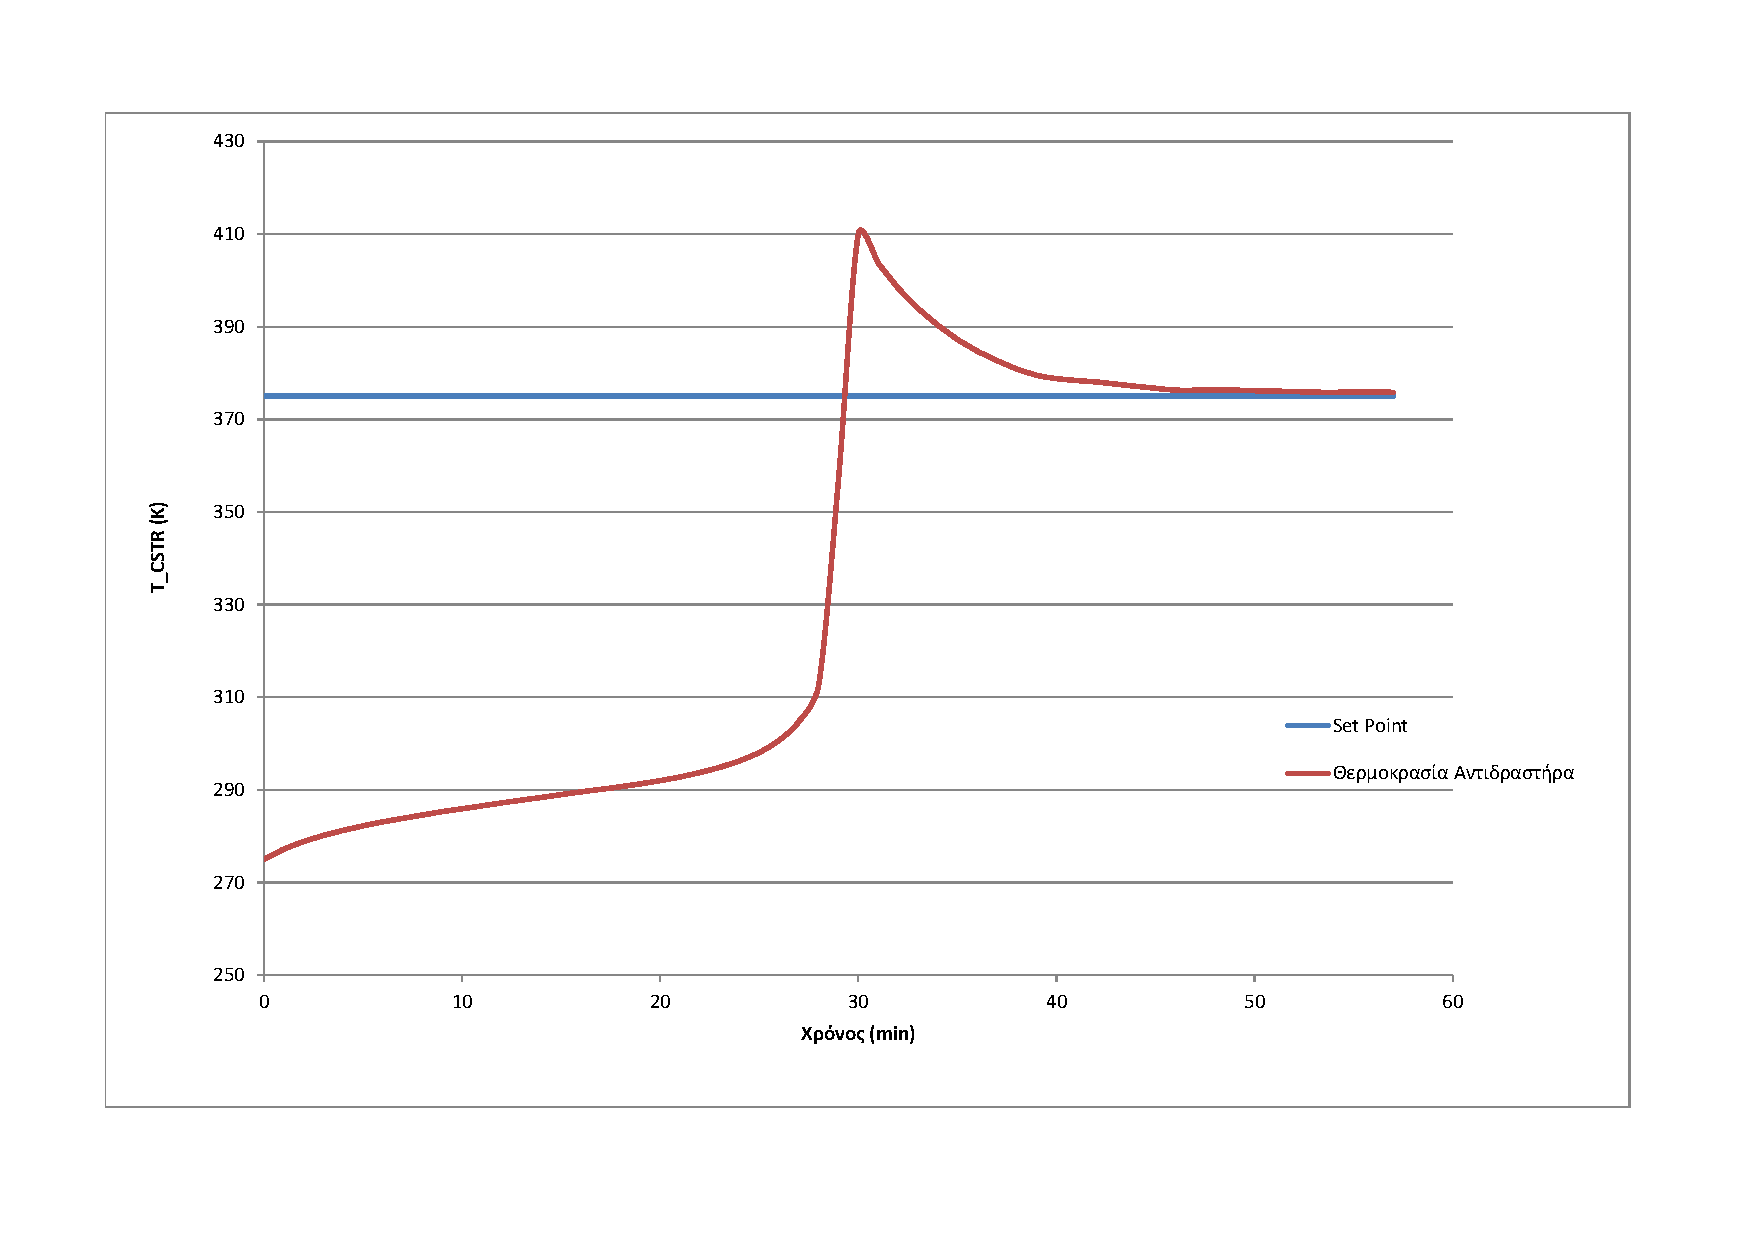
\includegraphics[width=0.8\textwidth]{noise_t.pdf}
    \caption{Προφίλ της θερμοκρασίας του αντιδραστήρα συναρτήσει του χρόνου με την χρήση θορύβου}
    \label{fig:noise_t}
\end{figure}

\begin{figure}[H]
    \centering
    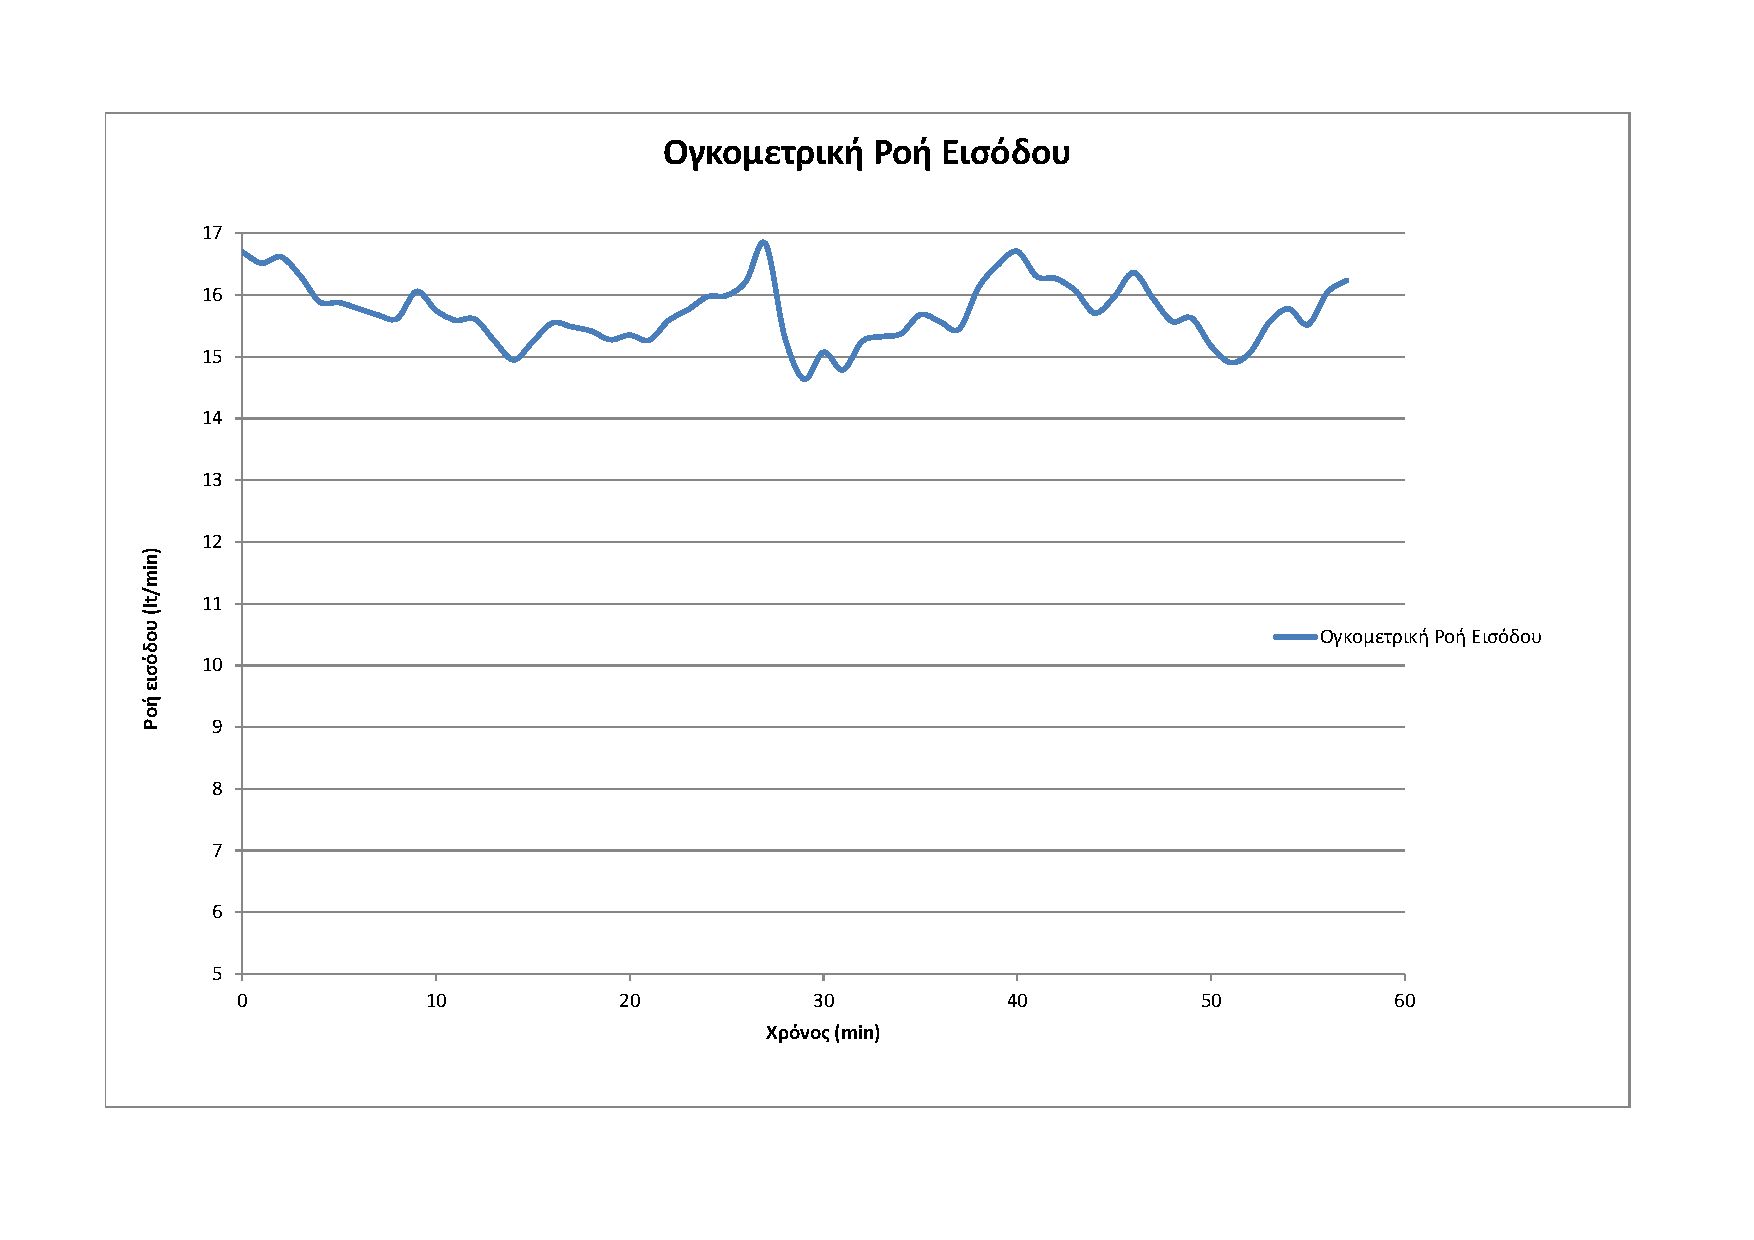
\includegraphics[width=0.8\textwidth]{noise_f.pdf}
    \caption{Προφίλ της ροής εισόδου συναρτήσει του χρόνου με την χρήση θορύβου}
    \label{fig:noise_f}
\end{figure}

\begin{figure}[H]
    \centering
    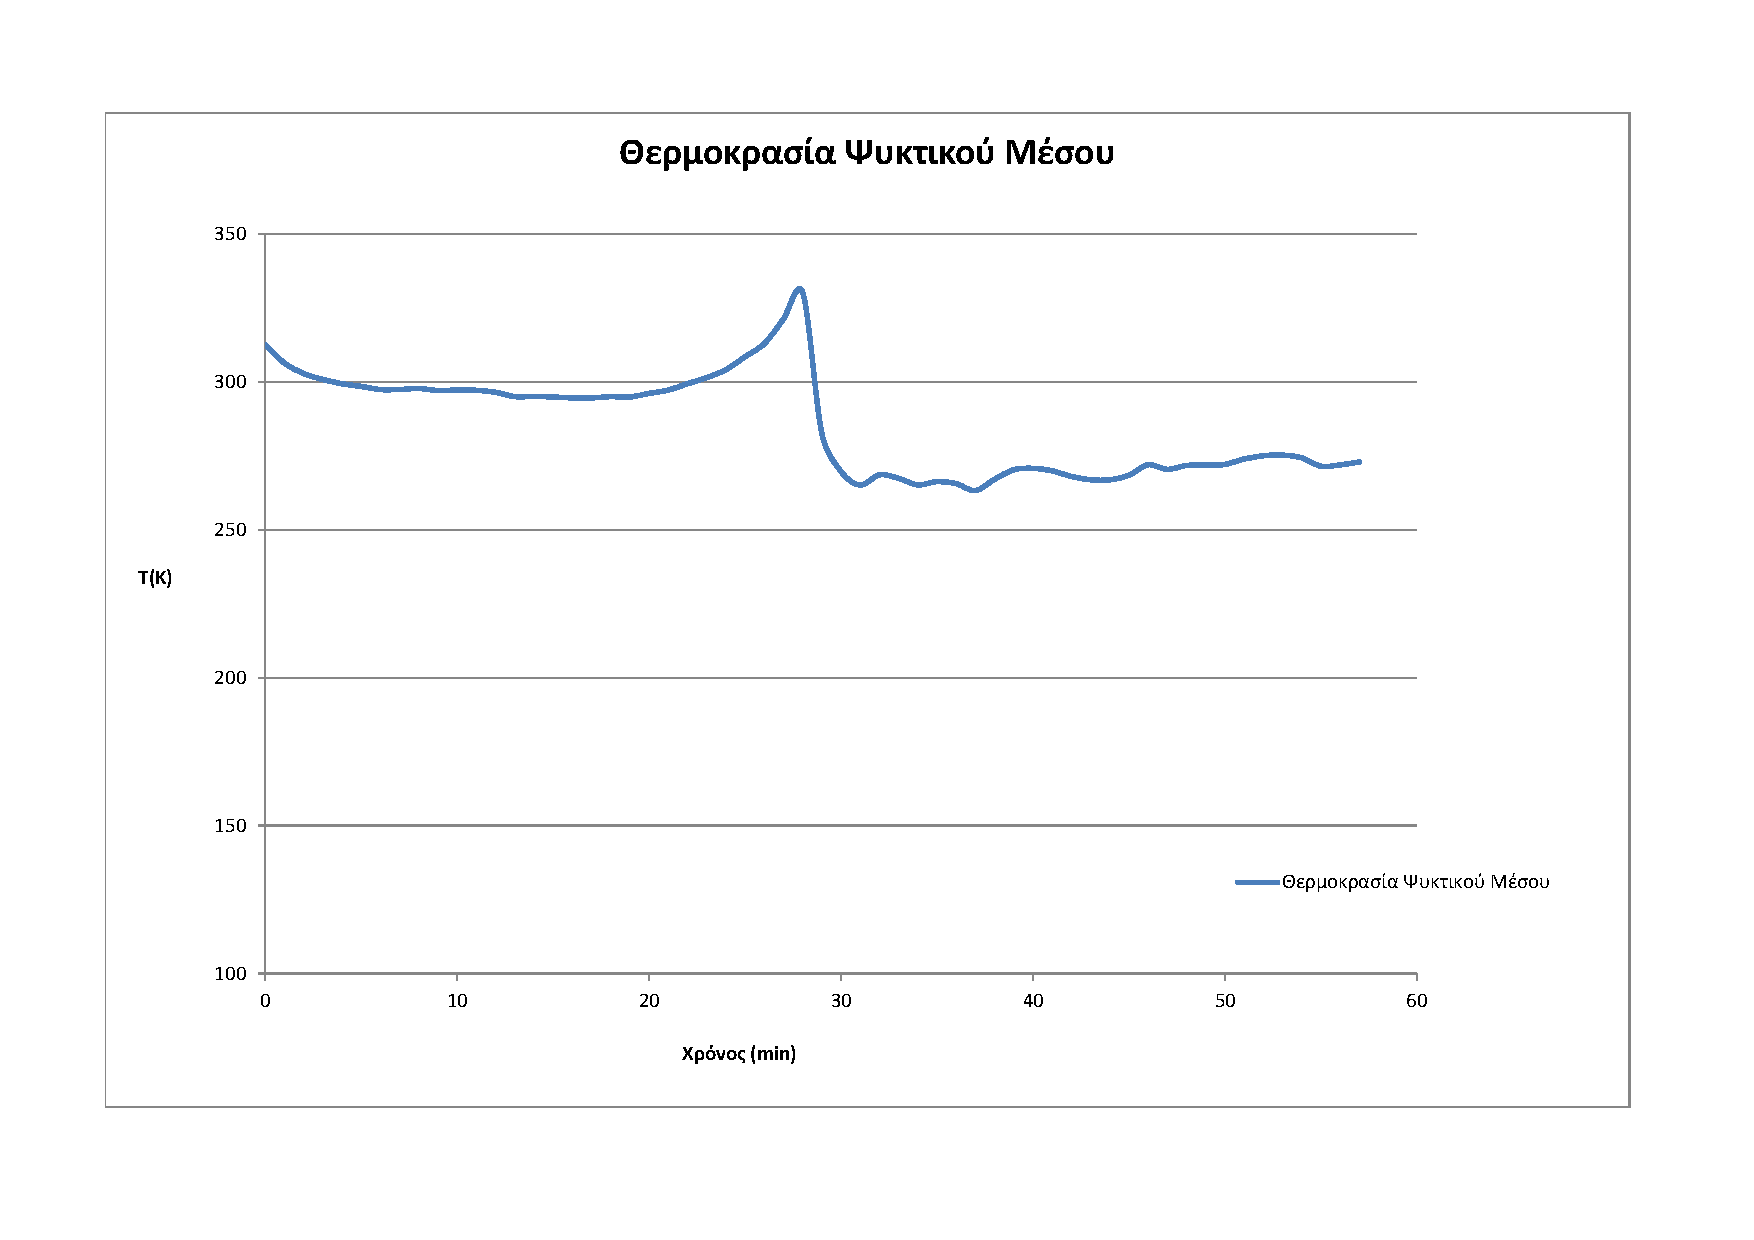
\includegraphics[width=0.8\textwidth]{noise_t_cool.pdf}
    \caption{Προφίλ της θερμοκρασίας του ψυκτικού μέσου συναρτήσει του χρόνου με την χρήση θορύβου}
    \label{fig:noise_t_cool}
\end{figure}

Ας παρατηρήσουμε για αρχή το τελικό αποτέλεσμα της εκπαίδευσης, δηλαδή τα διαγράμματα της συγκέντρωσης και της θερμοκρασίας του αντιδραστήρα. Βλέπουμε ότι περίπου μέχρι και το χρονικό βήμα 28 η συγκέντρωση του Α πέφτει με ομαλό και αργό ρυθμό και συνεπώς, εφόσον η αντίδραση είναι εξώθερμη, η θερμοκρασία του αντιδραστήρα ανεβαίνει και αυτή με έναν ομαλό ρυθμό. Στα χρονικά βήματα 29 και 30 όμως παρατηρείται μία πολύ απότομη κλίση στο διάγραμμα της συγκέντρωσης, όπου και φαίνεται ότι ο ρυθμός της αντίδρασης είναι μέγιστος. Στα ίδια χρονικά βήματα βλέπουμε ότι και η θερμοκρασία παρουσιάζει μία απότομη κλίση, ως αποτέλεσμα της απότομης μείωσης της συγκέντρωσης. Μάλιστα παρατηρείται και μία υπέρβαση τόσο στην συγκέντρωση όσο και στην θερμοκρασία. Μετά από την υπέρβαση αυτή η συγκέντρωση ανεβαίνει και πάλι, προσεγγίζει το επιθυμητό set point με πολύ μεγάλη ακρίβεια και παραμένει πολύ κοντά σε αυτό (εφόσον η αντίδραση είναι μονόδρομη δεν μπορεί να παράγεται Α μέσω της αντίδρασης οπότε το γιατί έχουμε αύξηση της συγκέντρωσής του Α θα το εξηγήσουμε με βάση τα διαγράμματα των δράσεων). Μάλιστα φαίνεται ότι το επισόδειο τελειώνει λίγο πριν το χρονικό βήμα 60, που σημαίνει ότι πληρείται η δεύτερη προϋπόθεση τερματισμού ενός επισοδείου. Ίδιες παρατηρήσεις κάνουμε και για την θερμοκρασία του αντιδραστήρα. Μετά την υπέρβαση, η οποία φαίνεται να φτάνει μέχρι τους 410Κ, η θερμοκρασία πέφτει, προσεγγίζει το set point και παραμένει πολύ κοντά σε αυτό. Συνεπώς φαίνεται ότι έχει επιτευχθεί μόνιμη κατάσταση, όπως και επιθυμούσαμε. Η μόνιμη αυτή κατάσταση μας εγγυάται μετατροπή του Α ίση με 93\% και θερμοκρασία εξόδου του αντιδραστήρα ίση με 375K.\\

Συνεχίζουμε με τα διαγράμματα των δράσεων. Παρατηρούμε ότι ο ρυθμιστής μας δίνει ένα αρκετά θορυβώδες προφίλ για την ροή εισόδου στον αντιδραστήρα. Το προφίλ αυτό δεν φαίνεται να παρουσιάζει κάποιο μοτίβο. Η μόνη παρατήρηση που μπορούμε να κάνουμε είναι ότι στα ίδια χρονικά βήματα που παρατηρείται η απότομη κλίση στο διάγραμμα της συγκέντρωσης και της θερμοκρασίας ο ρυθμιστής δίνει την εντολή για μία αυξημένη ροή εισόδου. Σε αυτήν την αυξημένη ροή οφείλεται και η αύξηση της συγκέντρωσης του Α αμέσως μετά την υπέρβαση. Εφόσον η αντίδραση είναι μονόδρομη, δεν μπορεί να παράγεται Α από την αντίδραση. Παρόλα αυτά η αυξημένη ροή εισόδου έχει ως αποτέλεσμα να εισέρχεται στον αντιδραστήρα μεγαλύτερη ποσότητα Α από αυτήν που παράγεται και εξέρχεται. Μέτα από το σημείο αυτό πάλι φαίνεται πως η ροή εισόδου δεν παρουσιάζει κάποιο συγκεκριμένο μοτίβο. Όσον αφορά την δράση της θερμοκρασίας του ψυκτικού φαίνεται ότι στα αρχικά στάδια του επισοδείου παραμένει σχεδόν σταθερή (αρχίζοντας από τους 310K και στην συνέχεια πέφτοντας γύρω στους 300K). Και σε αυτήν την περίπτωση στα χρονικά βήματα της απότομης κλίσης της συγκέντρωσης και της θερμοκασίας ο ρυθμιστής μας δίνει την εντολή για μία απότομη αλλαγή στην θερμοκρασία του ψυκτικού, η οποία παρουσιάζει ιδιαίτερο ενδιαφέρον. Σκοπός του ψυκτικού είναι να ρυθμίσει τις αυξήσεις της θερμοκρασίας του αντιδραστήρα λόγω του εξώθερμου της αντίδρασης. Παρόλα αυτά φαίνεται ότι εδώ ο ρυθμιστής δίνει εντολή για αύξηση θερμοκρασίας του ψυκτικού, παρά της αύξηση της θερμοκρασίας λόγω της πορείας της αντίδρασης. Σε αυτήν την δράση οφείλεται και η υπέρβαση στην θερμοκρασία του αντιδραστήρα και στην συγκέντρωση του Α. Φυσικά πρέπει να θυμόμαστε ότι ο ρυθμιστής δεν έχει καμία ενσωματωμένη έννοια του τί σημαίνει το να είναι μία αντίδραση εξώθερμη, ενδόθερμη ή της φυσικής σημασίας του συστήματος. Ο μοναδικός στόχος του ρυθμιστή είναι να κάνει ό,τι είναι απαραίτητο για να φτάσει το σύστημα μας στο επιθυμητό set point. Το μόνο που μπορούμε να κάνουμε είναι να τον καθοδηγήσουμε όσο πιο επιτυχημένα μπρορούμε στα set points αυτά με κατάλληλες συναρτήσεις κέρδους και άλλες παραμέτρους της μεθόδου. Μετά από την αύξηση αυτή της θερμοκρασίας του ψυκτικού ο ρυθμιστής δίνει την εντολή για απότομη μείωση της θερμοκρασίας, μιας και ανιχνεύει ήδη μία πολύ μεγάλη (σε σχέση με την επιθυμητή) θερμοκρασία του αντιδραστήρα. Μετά από την μείωση αυτή η θερμοκρασία του ψυκτικού φαίνεται να σταθεροποιείται σε μία θερμοκρασία κοντά στην περιοχή των 275Κ, όπου και επιτυγχάνεται η μόνιμη κατάσταση.\\

Το συμπέρασμα που εξάγουμε είναι ότι σε καθαρά θεωρητικό επίπεδο η ρύθμιση του συστήματος με ρυθμιστή βασισμένο στην προτεινόμενη μεθοδολογία είναι επιτυχής αφού η μόνιμη κατάσταση των μεταβλητών εξόδου επιτυγχάνεται με πολύ μεγάλη ακρίβεια. Παρόλα αυτά κρίνεται σκόπιμο να αναφερθεί ότι σε πρακτικό επίπεδο τα πράγματα ίσως να μην είναι τόσο εύκολα. Για αρχή θα πρέπει να είμαστε σίγουροι ότι ο αντιδραστήρας μας θα μπορεί να αντέξει αυτές τις υπερβάσεις της θερμοκρασίας. Επίσης θα πρέπει η βιομηχανία να μπορεί να διαθέσει ψυκτικό που να φτάνει τις θερμοκρασίες που δίνει ο ρυθμιστής. Τέλος θα πρέπει να ελεγθεί κατά πόσο είναι εφικτό αυτό το θορυβώδες προφίλ της ροής εισόδου στον αντιδραστήρα να επιτευχθεί στην πράξη. \\

Συνεχίζουμε με τα αποτελέσματα που προκύπτουν χωρίς την εισαγωγή του θορύβου κατά Ornstein-Uhlenbeck:\\

\begin{itemize}
\item $C_{A_{set}} = 0.07$ , $Τ_{set} = 375$ χωρίς την χρήση θορύβου κατά Ornstein-Uhlenbeck
\end{itemize}
Όλες οι υπόλοιπες παράμετροι της προσομοίωσης παραμένουν οι ίδιες. Η μόνη αλλαγή που κάνουμε είναι να αφαιρέσουμε την συνιστώσα του θορύβου Ornstein-Uhlenbeck από την δράση. Τα καινούρια αποτελέσματα φαίνονται στα παρακάτω διαγράμματα:
\begin{figure}[H]
    \centering
    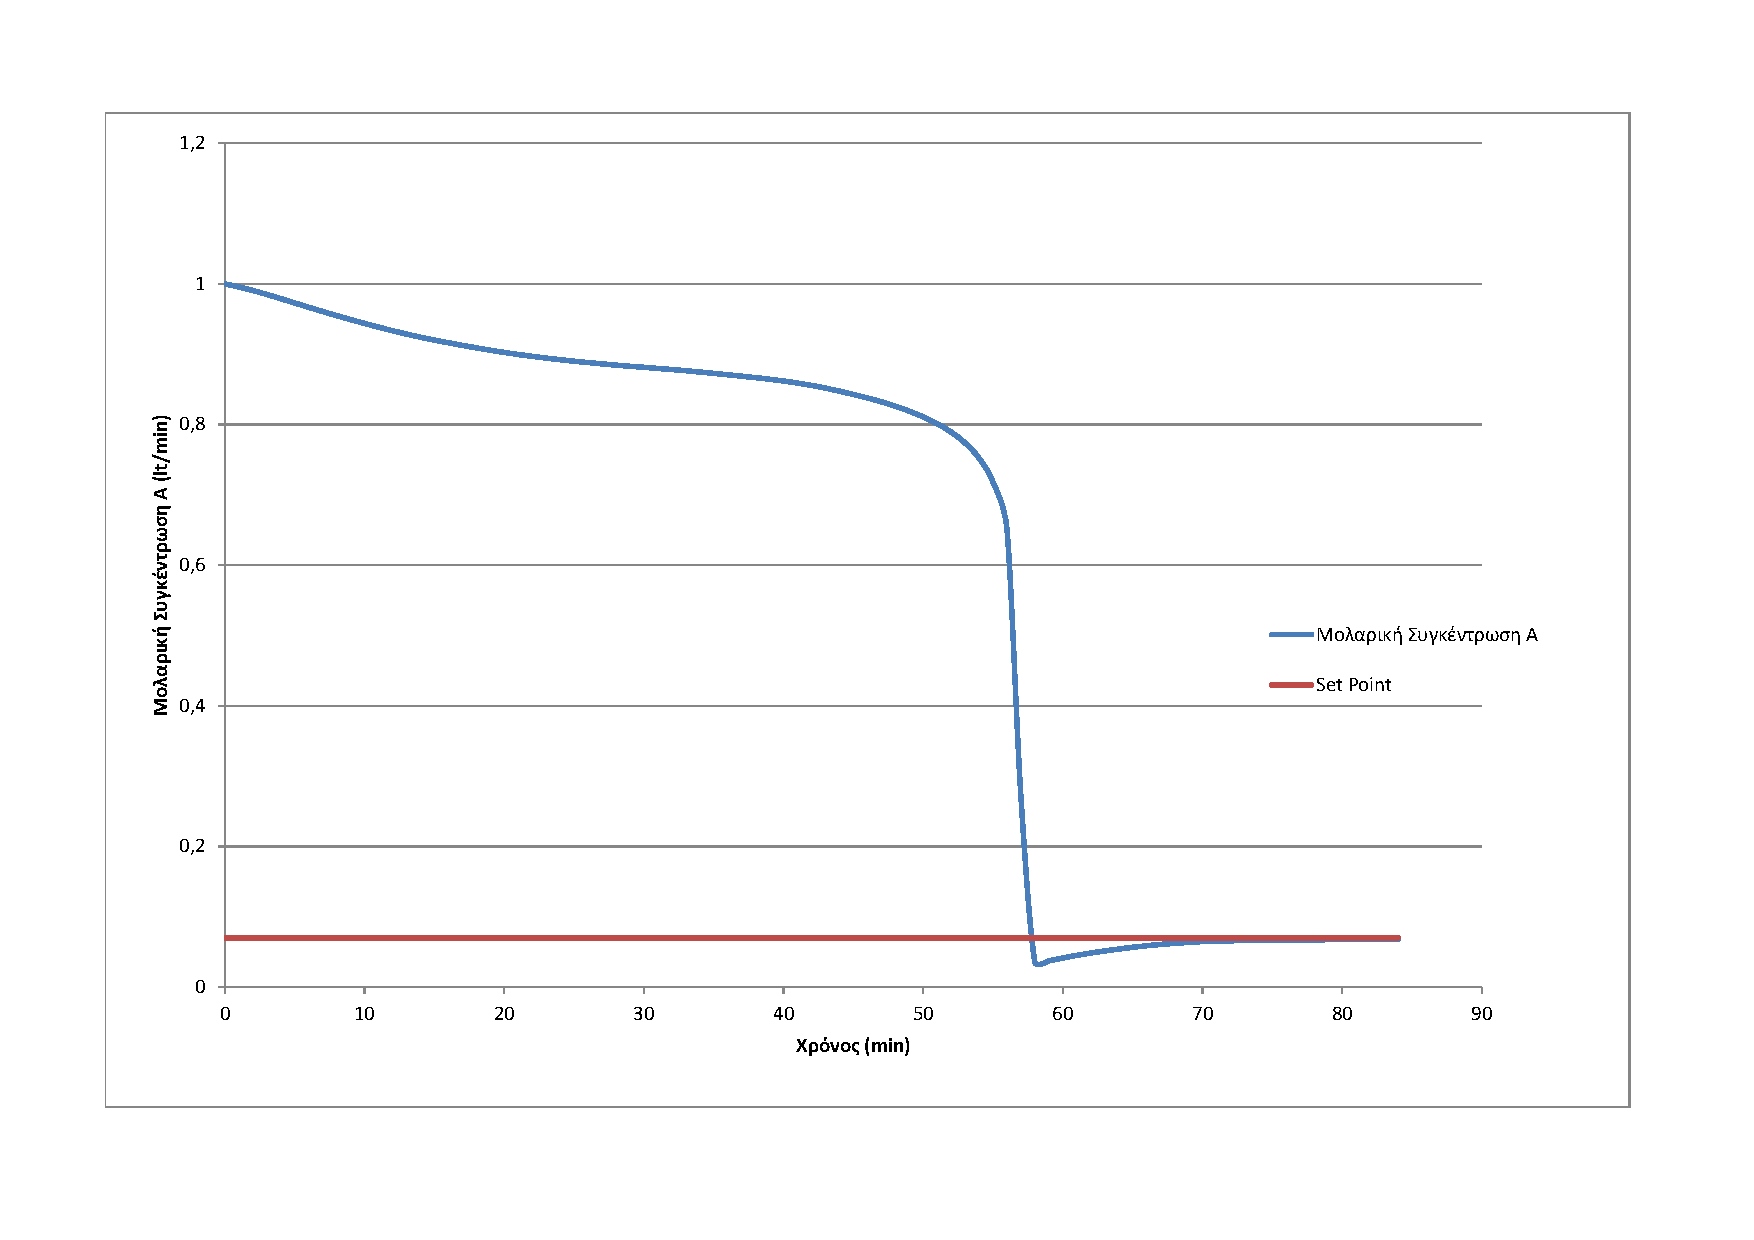
\includegraphics[width=0.8\textwidth]{no_noise_ca.pdf}
    \caption{Προφίλ της συγκέντρωσης του Α συναρτήσει του χρόνου χωρίς την χρήση θορύβου}
    \label{fig:no_noise_ca}
\end{figure}

\begin{figure}[H]
    \centering
    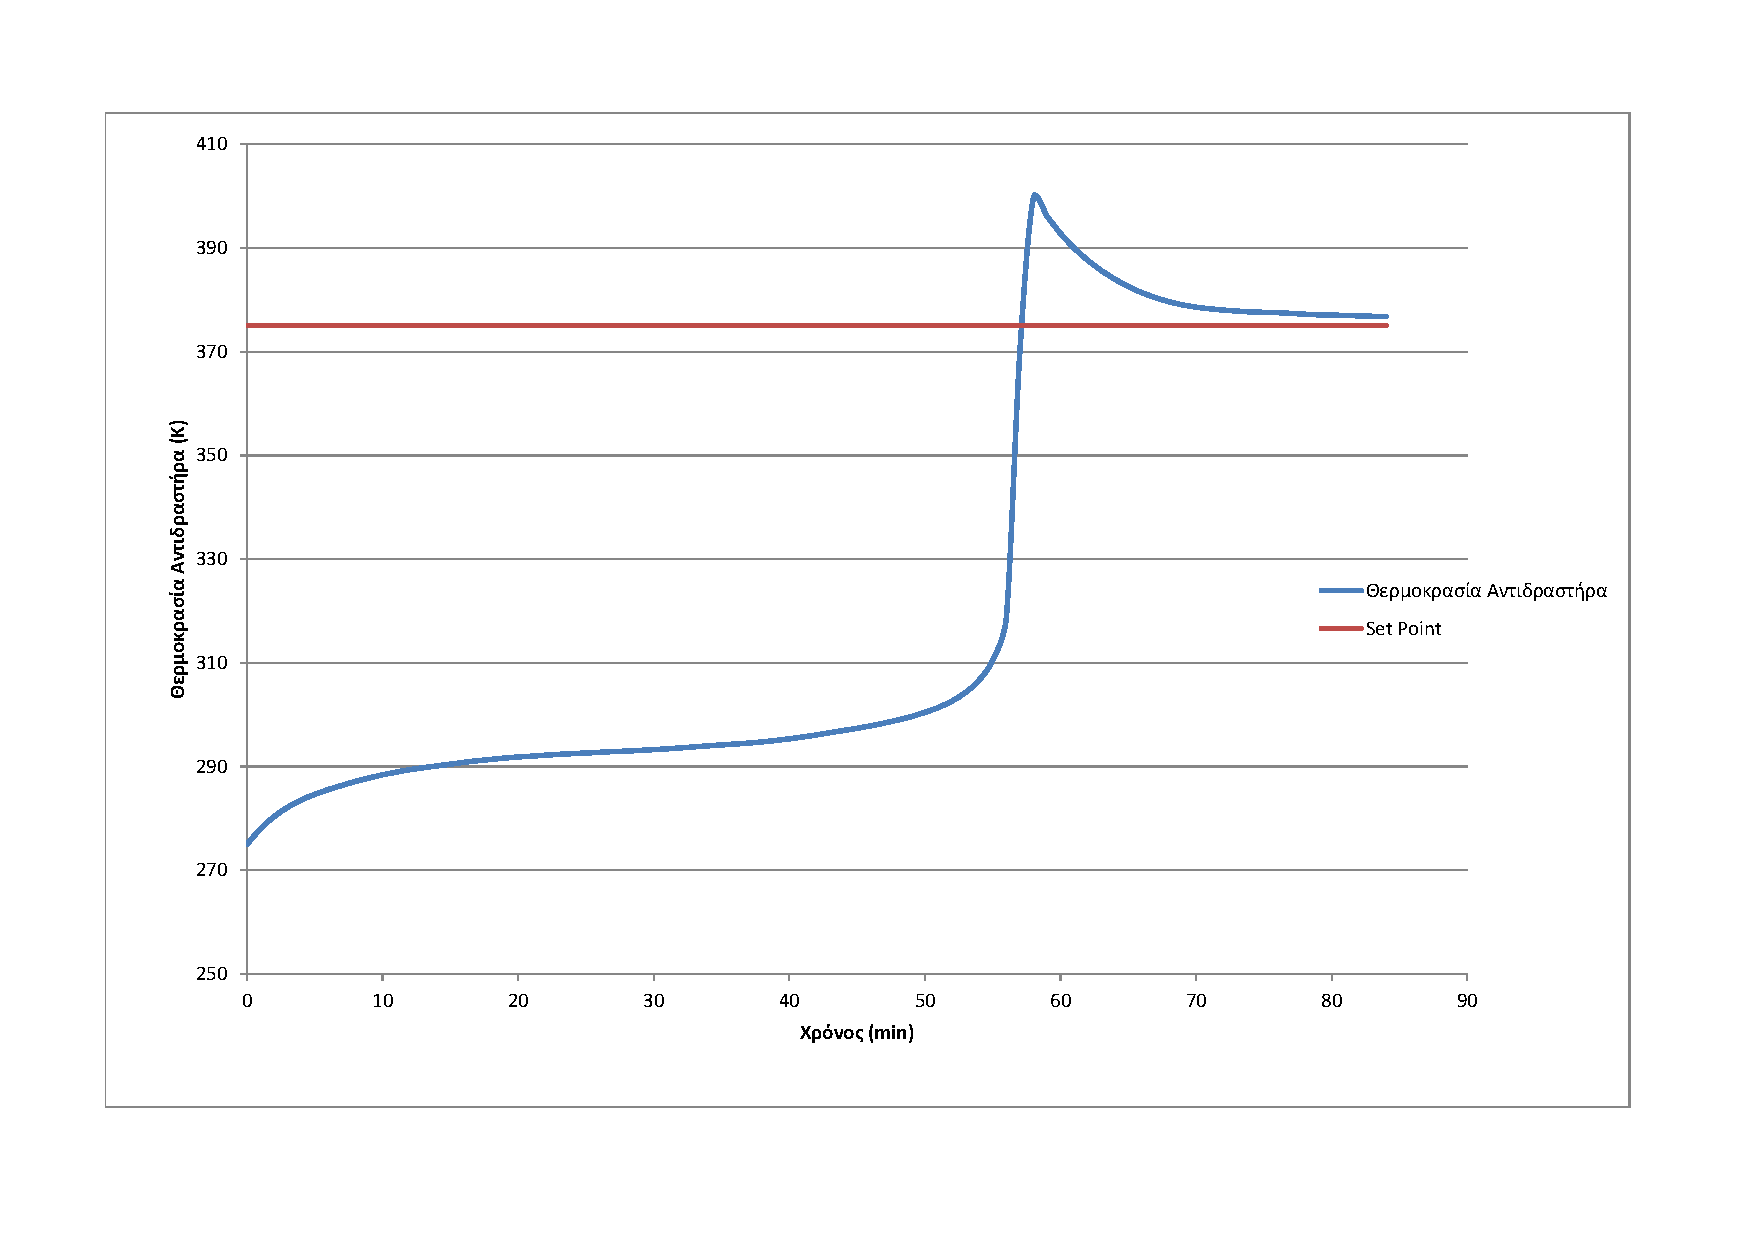
\includegraphics[width=0.8\textwidth]{no_noise_t.pdf}
    \caption{Προφίλ της θερμοκρασίας του αντιδραστήρα συναρτήσει του χρόνου χωρίς την χρήση θορύβου}
    \label{fig:no_noise_t}
\end{figure}

\begin{figure}[H]
    \centering
    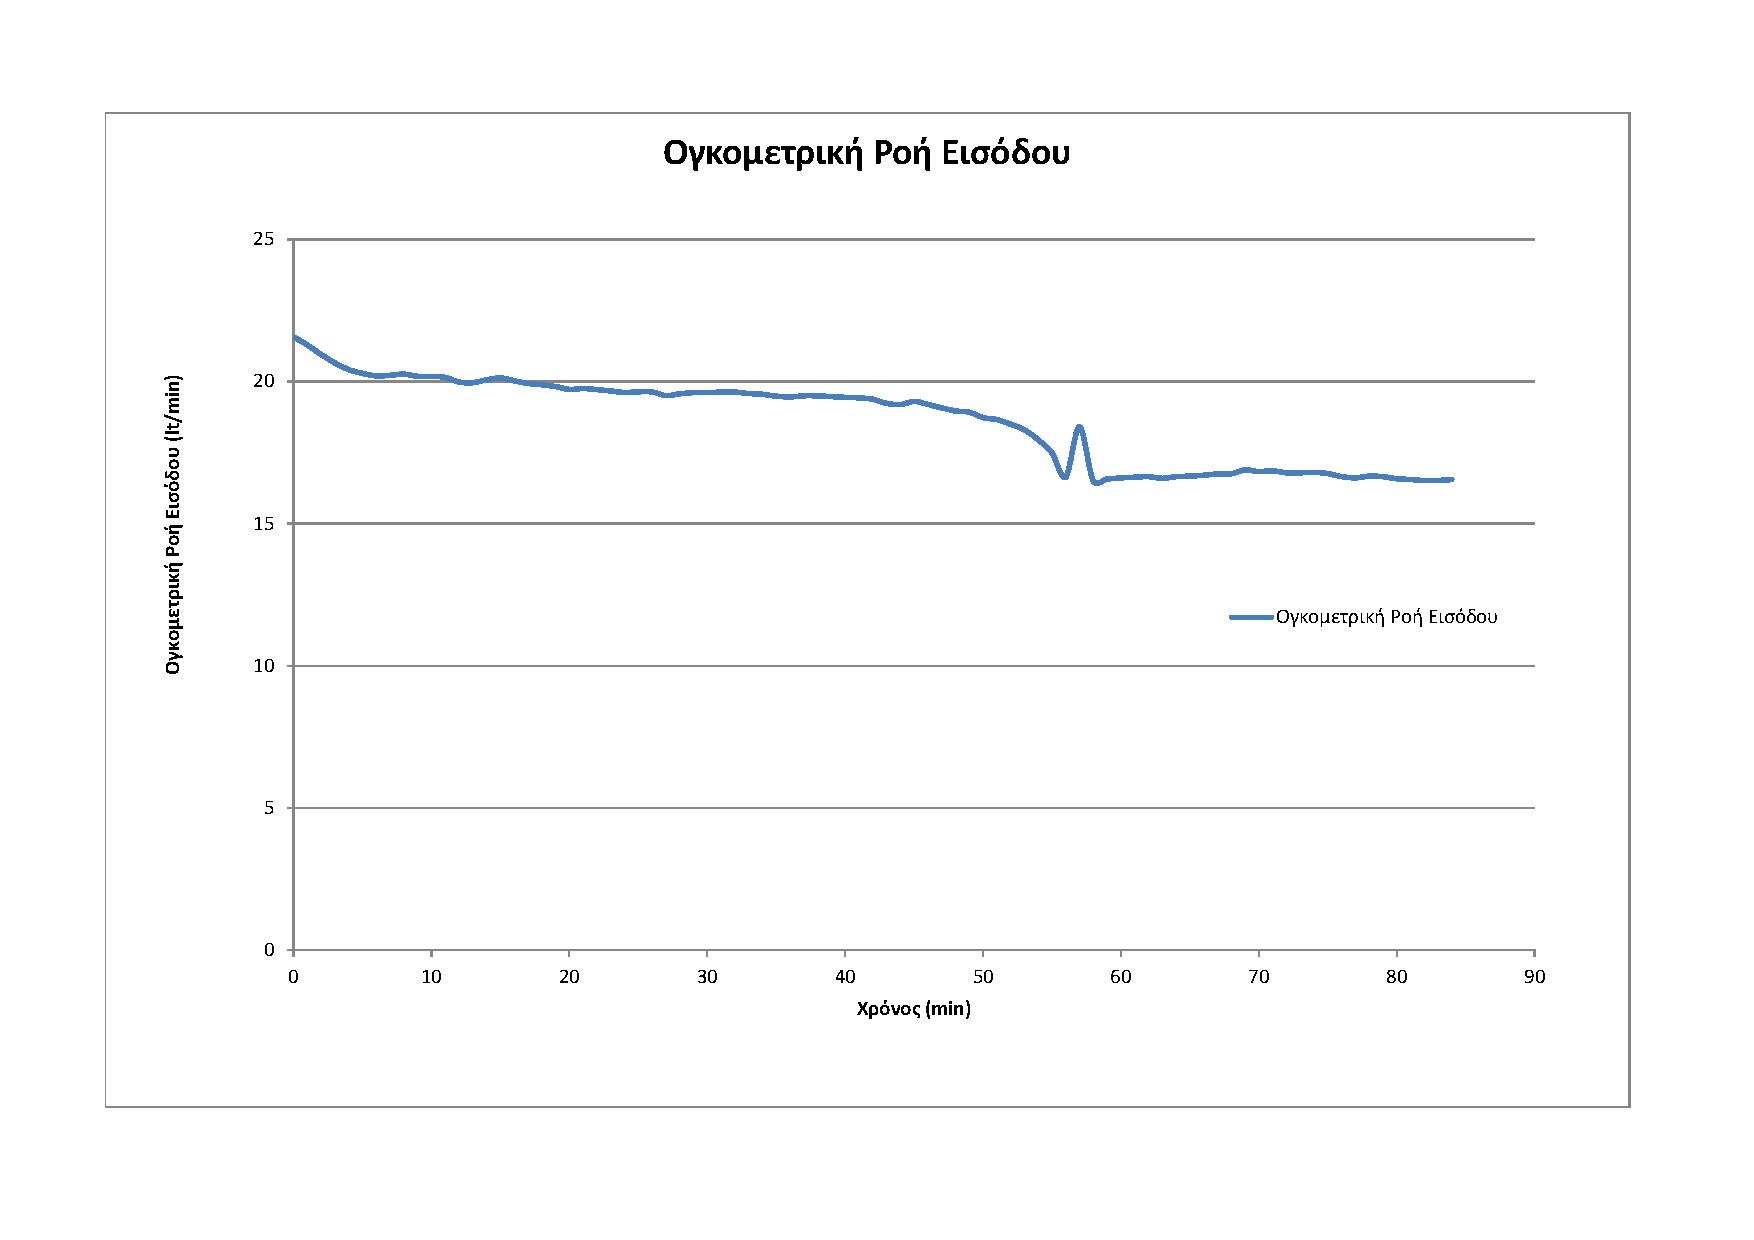
\includegraphics[width=0.8\textwidth]{no_noise_f.pdf}
    \caption{Προφίλ της ροής εισόδου συναρτήσει του χρόνου χωρίς την χρήση θορύβου}
    \label{fig:no_noise_f}
\end{figure}

\begin{figure}[H]
    \centering
    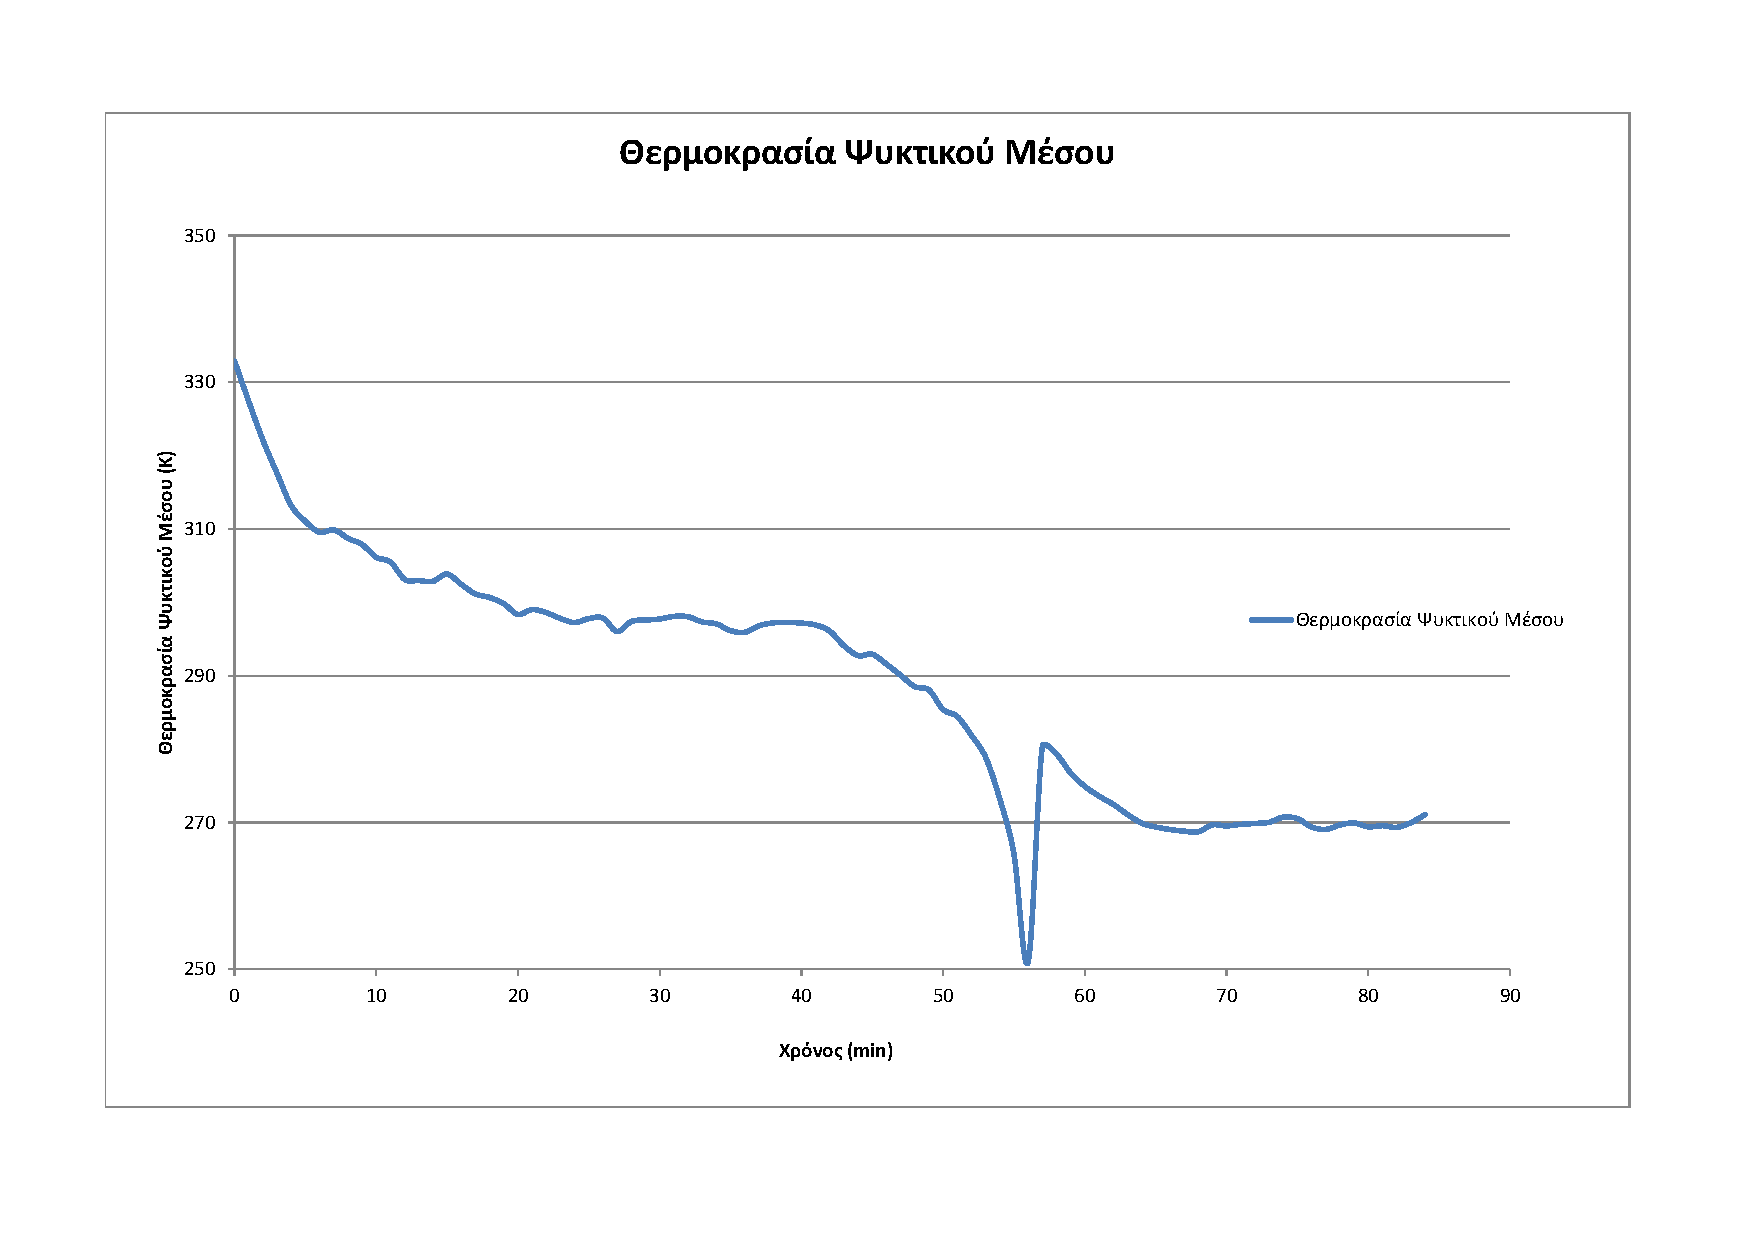
\includegraphics[width=0.8\textwidth]{no_noise_t_cool.pdf}
    \caption{Προφίλ της θερμοκρασίας του ψυκτικού συναρτήσει του χρόνου χωρίς την χρήση θορύβου}
    \label{fig:noise_ca}
\end{figure}

Με μία γρήγορη ματιά στα παραπάνω διαγράμματα τα αποτελέσματα είναι πολύ πιο αισιόδοξα, κυρίως όσον αφορά το προφίλ των δράσεων, σε σχέση με αυτά που προέκυψαν με την εισαγωγή της συνιστώσας του θορύβου Ornstein-Uhlenbeck. Ας αρχίσουμε όμως για αρχή να παρατηρούμε τα διαγράμματα των μεταβλητών εξόδου.\\

Παρατηρούμε ότι η συμπεριφορά τόσο της συγκέντρωσης του Α όσο και της θερμοκρασίας του αντιδραστήρα είναι πολύ παρόμοια με αυτήν που προέκυψε από την χρήση του θορύβου. Υπάρχει όμως μία ουσιώδης διαφορά. Η περιοχή της απότομης μεταβολής της συγκέντρωσης και της θερμοκρασίας βρίσκεται τώρα κοντά στο χρονικό βήμα 58 και 59, σε αντίθεση με την προηγούμενη περίπτωση όπου παρατηρούσαμε αυτήν την απότομη αλλαγή περίπου στο χρονικό βήμα 29. Αυτή η χρονική καθυστέρηση έχει μία θετική συνέπεια στην εκπαίδευση και την ρύθμιση του συστήματος. Αν συγκρίνουμε, για παράδειγμα, τα διαγράμματα της συγκέντρωσης του Α με και χωρίς την χρήση θορύβου θα παρατηρήσουμε ότι στο σημείο που αρχίζει η απότομη κλίση του διαγράμματος στην περίπτωση της μη-χρήσης του θορύβου είναι μικρότερη σε σχέση με την συγκέντρωση στην περίπτωση του θορύβου. Αυτό συμβαίνει γιατί, λόγω της χρονικής αυτής υστέρησης στην δεύτερη περίπτωση, η αντίδραση προλαβαίνει να προχωρήσει λίγο παραπάνω, ρίχνοντας έτσι περισσότερο την συγκέντρωση του Α. Η θετική συνέπεια αυτής της παρατήρησης είναι το γεγονός ότι η υπέρβαση που παρατηρείται, τόσο στην συγκέντρωση όσο και στην θερμοκρασία, είναι μικρότερη σε σχέση με την υπέρβαση που παρατηρούσαμε όταν ήταν παρών και ο θόρυβος. Στην περίπτωση της θερμοκρασίας του αντιδραστήρα, για παράδειγμα, ο θόρυβος οδηγούσε σε μία υπέρβαση που έφτανε τους 410Κ ενώ η εξαγωγή του θορύβου μείωσε την υπέρβαση αυτή κατά 10 περίπου βαθμούς. Φυσικά και σε αυτήν την περίπτωση θα πρέπει να σιγουρευτούμε ότι ο αντιδραστήρας μας θα μπορεί να αντέξει τις υψηλές αυτές θερμοκρασίες. Μετά από αυτές τις υπερβάσεις, η συγκέντρωση και η θερμοκρασία επανέρχονται με ομαλό τρόπο στα set points και συγκλίνουν σε αυτά. Συνεπώς και σε αυτήν την περίπτωση πετύχαμε μόνιμη κατάσταση και η ρύθμιση ήταν επιτυχής, σε θεωρητικό επίπεδο προς το παρόν. Μέχρι τώρα εξετάσαμε το αποτέλεσμα του ρυθμιστή μας. Συνεχίζουμε τώρα με τα διαγράμματα των δράσεων, δηλαδή τις εντολές του ίδιου του ρυθμιστή.\\

Για αρχή δεν μπορεί κανέις παρά να παρατηρήσει την τεράστια διαφορά του προφίλ της ροής εισόδου του αντιδραστήρα. Στην τρέχουσα περίπτωση η ροή εισόδου παρουσιάζει μία πολύ πιο ομαλή συμπεριφορά η οποία έχει πάψει να χαρακτηρίζεται από το θορυβώδες προφίλ της περίπτωσης του θορύβου. Στην αρχή του επισοδείου, όπου παρατηρείται και η ομαλή μεταβολή της συγκέντρωσης, η ροή εισόδου φαίνεται να έχει μία πτωτική -σχεδόν σταθερή- συμπεριφορά. Η μόνη παρατήρηση που μπορούμε να κάνουμε είναι η εντολή της πτώσης της ροής και της μικρής κορυφής που δίνει ο ρυθμιστής ακριβώς στην περιοχή της απότομης μεταβολής των μεταβλητών εξόδου. Είναι και ο λόγος που μετά την μικρή υπέρβαση η συγκέντρωση του Α ανεβαίνει. Μετά την κορυφή αυτή η ροή εισόδου φτάνει και αυτή σε μόνιμη κατάσταση και σταθεροποιείται περίπου στα $16.5 \frac{lt}{min}$. \\

Όσον αφορά την θερμοκρασία του ψυκτικού φαίνεται να παρουσιάζει σχεδόν εξ'ολοκλήρου μία πτωτική συμπεριφορά. Όταν η συγκέντρωση του Α μεταβάλλεται πολύ απότομα (κοντά στο χρονικό βήμα 58) ο ρυθμιστής δίνει την εντολή για μία ραγδαία πτώση της θερμοκρασία του ψυκτικού. Η συμπεριφορά αυτή είναι πιο κοντά στην διαίσθησή μας.  Εφόσον η αντίδραση είναι εξώθερμη, στις περιοχές απότομης μείωσης της συγκέντρωσης (δηλαδή σε περιοχές μεγάλου ρυθμού αντίδρασης) αναμένουμε και μεγάλες αυξήσεις στην θερμοκρασία (όπως επιβεβαιώνεται και από το διάγραμμα της θερμοκρασίας του αντιδραστήρα). Συνεπώς εκείνο είναι το σημείο όπου ο ρυθμιστής πρέπει να λάβει δράση για να μειώσει την θερμοκρασία του αντιδραστήρα όσο πιο γρήγορα μπορεί. Εμφανίζεται λοιπόν αυτή η μικρή κορυφή στην θερμοκρασία του ψυκτικού, η οποία διαρκεί για μόλις δύο χρονικά βήματα. Αυτή είναι και η μεγαλύτερη διαφορά που μπορούμε να διακρίνουμε όταν συγκρίνουμε τα διαγράμματα της συμπεριφοράς της θερμοκρασίας του ψυκτικού. Στην περίπτωση του θορύβου ο ρυθμιστής δίνει εντολή για μία \textit{αύξηση} της θερμοκρασίας του ψυκτικού, κάτι που όντως προκαλεί έκπληξη στην αρχή. Αυτή η αύξηση της θερμοκρασίας είναι και ο λόγος που η υπέρβαση στην περίπτωση του θορύβου είναι μεγαλύτερη από την υπέρβαση της θερμοκρασίας όταν δεν έχουμε θόρυβο, όπου ο ρυθμιστής δίνει εντολή για μείωση της θερμοκρασίας του ψυκτικού στην περιοχή υψηλού ρυθμού αντίδρασης. Μετά από την κορυφή αυτή, ο ρυθμιστής αυξάνει και πάλι την θερμοκρασία του ψυκτικού και στην συνέχεια την ρίχνει με ομαλό ρυθμό, όπου και συγκλινει κοντά στους 270K.\\

Αυτό που μπορούμε να συμπεράνουμε είναι ότι η εξαγωγή της συνιστώσας του θορύβου κατά Ornstein-Uhlenbeck έχει αρκετά πλεονεκτήματα και ένα μειονέκτημα. Το βασικό μειονέκτημα είναι ότι η ρύθμιση του συστήματος παρουσιάζει μία χρονική υστέρηση της τάξεως των 20 χρονικών βημάτων, που στην συγκεκριμένη περίπτωση σημαίνει χρονική υστέρηση 20 λεπτών. Τα 20 λεπτά αυτά μπορεί να είναι κρίσιμα για την διεργασία ή/και για το χρονοδιάγραμμα της βιομηχανίας που χρησιμοποιεί τον προτεινόμενο ρυθμιστή. Στα πλεονεκτήματα φυσικά ανήκουν οι μικρότερες υπερβάσεις των μεταβλητών εξόδου καθώς και τα πολύ πιο ομαλά προφίλ των μεταβλητών εισόδου (ροή και θερμοκρασία ψυκτικού). Το δεύτερο είναι αρκετά πιο σημαντικό καθώς τώρα μπορεί να μπει και στο παιχνίδι η πιθανή πρακτική εφαρμογή ενός τέτοιου ρυθμιστή. \\

Είναι δύσκολο να εξηγηθεί με πλήρη μαθηματική ακρίβεια \textit{γιατί} τα αποτελέσματα που παίρνουμε όταν βγάζουμε τον θόρυβο κατά Ornstein-Uhlenbeck είναι διαφορετικά (και στην συγκεκριμένη περίπτωση καλύτερα). Η ουσία είναι ότι με την χρήση του θορύβου ο πράκτορας-ρυθμιστής \textit{εξερευνεί} τον χώρο με διαφορετικό τρόπο σε σχέση με την περίπτωση απουσίας του. Η διαφορετική αυτή εξερεύνηση ενδέχεται να δίνει στον πράκτορα έναν διαφορετικό τρόπο βελτιστοποίησης και ρύθμισης του συστήματος, ο οποίος να επιφέρει \textit{μεγαλύτερο κέρδος στο τέλος του επισοδείου}. Θα πρέπει εν τέλει να θυμόμαστε ότι ο πράκτορας δεν έχει καμία έννοια του τι σημαίνει φυσικό σύστημα, φυσική σημασία κ.τ.λ. Πρόκειται για ένα πρόγραμμα στον υπολογιστή το οποίο είναι προγραμματισμένο να μαζέψει κατά το δυνατόν περισσότερο κέρδος ελαχιστοποιώντας τις συναρτήσεις κόστους. Κατά πάσα πιθανότητα ο πράκτορας μαζεύει περισσότερο κέρδος στην περίπτωση του θορύβου όταν εξερευνεί τον χώρο με τον τρόπο που είδαμε. Φυσικά ο τρόπος αυτός έχει ως αποτέλεσμα ένα χειρότερο σύστημα ρύθμισης, από πρακτικής μεριάς.\\

\section{Συμπεράσματα και σχολιασμοί}
Ως πρώτο σχόλιο θα πρέπει να αναφερθεί ότι τα παραπάνω αποτελέσματα κατά πάσα πιθανότητα δεν είναι τα βέλτιστα δυνατά. Όπως έγινε εμφανές από τις παραπάνω προσομοιώσεις, η προτεινόμενη μεθοδολογία DDPG είναι αρκετά ευαίσθητη σε πολλές από τις παραμέτρους που εμφανίζονται. Είδαμε πως μία μικρή αλλαγή στην συνάρτηση κέρδους και η εξαγωγή του τυχαίου περιπάτου Ornstein-Uhlenbeck αλλάζει αρκετά τα αποτελέσματα της προσομοίωσης. Ο αλγόριθμος αυτός είναι ακόμη καινούριος (της τελευταίας πενταετίας) και δεν είναι απίθανο στο μέλλον να βρεθούν τροποποιήσεις και βελτιώσεις. Επίσης θα πρέπει να αναφερθεί ότι ο αλγόριθμος αυτός δεν αποτελεί πανάκεια των σύγχρονων συστημάτων ρύθμισης. Προς το παρόν έχει δοκιμασθεί κυρίως σε γραμμικά μοντέλα και πάντα σε θεωρητικό επίπεδο. Απέχουμε ίσως και αρκετά χρόνια μέχρι οι ρυθμιστές βασισμένοι σε τεχνιτή νοημοσύνη να βρουν επίσημη θέση στη βιομηχανία. Παρακάτω παρουσιάζονται συγκεντρωτικά τα συμπεράσματα που βγήκαν από την μελέτη που προηγήθηκε:\\
\begin{itemize}
\item Η συνάρτηση κέρδους $r(s, \alpha, s')$ είναι μία πολύ ευαίσθητη παράμετρος του αλγορίθμου και πολλές φορές μπορεί να χρειαστεί αρκετή σκέψη και δοκιμές μέχρι να βρεθεί η κατάλληλη. Δεν αποκλείεται να υπάρχουν συναρτήσεις κέρδους που να δίνουν καλύτερα αποτελέσματα σε σχέση με αυτά που παρουσιάσθηκαν σε αυτήν την εργασία\\
\item Η εισαγωγή του θορύβου κατά Ornstein-Uhlenbeck δεν συνεπάγεται απαραίτητα καλύτερη εκπαίδευση με την πρακτική έννοια της ρύθμισης του συστήματος. Παρόλο που μπορεί να προσφέρει αποδοτικότερη και ταχύτερη εξερεύνηση του χώρου στον οποίο ζει η διεργασία δεν σημαίνει ότι απο πρακτικής σκοπιάς θα είναι και η προτιμέστερη επιλογή\\
\item Οι υπολογιστικοί χρόνοι είναι πολύ μεγαλύτεροι προφανώς σε πολυμεταβλητά και μη-γραμμικά συστήματα. Ενδεικτικά, στην εν λόγω εργασία, στο μονομεταβλητό $1 \times 1$ σύστημα ο αλγόριθμος μπόρεσε να συγκλίνει και να επιτύχει μόνιμη κατάσταση εντός περίπου μισής ώρας (ίσως και λίγο λιγότερο). Στο πολυμεταβλητό σύστημα ο αλγόριθμος χρειάστηκε πολύ περισσότερο χρόνο για να δώσει τα παραπάνω αποτελέσματα, περίπου μιάμιση ώρα. Παρατηρήθηκε επίσης ότι η εισαγωγή του θορύβου μείωσε για πολύ λίγο τον υπολογιστικό χρόνο\\
\item Δεν είναι όλοι οι βελτιστοποιητές κατάλληλοι για όλα τα συστήματα που επιχειρούμε να ρυθμίσουμε. Για παράδειγμα ο Adam Optimizer έδειξε πολύ κακή συμπεριφορά στο πολυμεταβλητό σύστημα ενώ τελικά την δουλειά την έκανε ο GradientDescentOptimizer. Το ποιος βελτιστοποιητής είναι ο καταλληλότερος είναι θέμα εμπειρίας και δοκιμής και σφάλματος  
\item Σε όλες τις υπο εξέταση περιπτώσεις παρατηρείται μία υπέρβαση πάνω ή κάτω από το επιθυμητό set point. Το επόμενο βήμα λοιπόν είναι η λεπτομερέστερη διερεύνηση των παραμέτρων του αλγορίθμου για να διαπιστωθεί ποια είναι αυτή που οδηγεί σε αυτές τις υπερβάσεις με σκοπό φυσικά την μείωση (ή ακόμα και την εξάλειψη) του μέτρου των υπερβάσεων αυτών. Μία πρώτη σκέψη είναι να ελέγξουμε ποια είναι η κοινή παράμετρος ή οι κοινές παράμετροι που δεν άλλαξαν κατά την διάρκεια των προσομοιώσεων και να δοκιμάσουμε να αλλάξουμε αυτές. Στην προκειμένη περίπτωση σε όλες τις προσομοιώσεις χρησιμοποιήθηκε η ίδια συνάρτηση κόστους (συνάρτηση μέσου τετραγωνικού σφάλματος), ο ίδιος βελτιστοποιητής (GradientDescentOptimizer) και ο ίδιος ρυθμός εκμάθησης (η παράμετρος \tau) των νευρωνικών δικτύων. Συνεπώς προτείνεται ο πειραματισμός και περαιτέρω προσομοιώσεις με την μεταβολή μίας κάθε φορά από τις παραπάνω παραμέτρους (και σε επόμενο στάδιο συνδυασμός αυτών ή και περισσότερων παραμέτρων).
\end{itemize}

\newpage
 
\section{Παράρτημα}

\subsection{Θεώρημα Σταθερού Σημείου του Banach}
Για να διατυπώσουμε αλλά και να αποδείξουμε το Θεώρημα Σταθερού Σημείου του Banach θα πρέπει να δώσουμε κάποιους ορισμούς αλλά και να αποδείξουμε δύο μικρά λήμματα.\\

\textbf{Ορισμός}: Έστω $(\textbf{X}, d)$ ένας μετρικός χώρος. Μία απεικόνιση $\textbf{T}: \textbf{X} \rightarrow \textbf{X}$ καλείται \textit{συστολή} στον \textbf{X} αν υπάρχει $c \in [0, 1)$ τέτοιος ώστε:
\begin{align*}
d(\textbf{T}(x), \textbf{T}(y)) \leq c d(x, y), \hspace{1cm} \forall  x,y \in \textbf{X}
\end{align*}

\textbf{Λήμμα 1}: Έστω $(\textbf{X}, d)$ ένας μετρικός χώρος, \textbf{T} μία συστολή στον \textbf{X} και $x_{0} \in \textbf{X}$. Ορίζουμε ακολουθία $\{x_n\}$ στον \textbf{X} ως $x_{n} = \textbf{T}(x_{n-1})$. Τότε ισχύει ότι
\begin{equation}
d(x_{n+1}, x_{n}) \leq c^{n} d(x_{1}, x_{0}) \hspace{1cm} \forall n \in \mathbb{N}
\end{equation}
\textbf{Απόδειξη}:\\
Η απόδειξη θα γίνει με επαγωγή στο $n$. \\
\begin{itemize}
\item $n = 0$
\end{itemize}
\begin{align*}
d(x_{2}, x_{1})  = d(\textbf{T}(x_{1}), \textbf{T}(x_{2})) \leq c^{1} d(x_{1}, x_{0})
\end{align*}

Έστω τώρα ότι ισχύει για τυχαίο $n \in \mathbb{N}$, δηλαδή έχουμε σαν δεδομένο ότι $d(x_{n+1}, x_{n}) \leq c^{n} d(x_{1}, x_{0})$ (επαγωγική υπόθεση). Θα δείξουμε ότι ισχύει για $n+1$. Πράγματι
\begin{align*}
d(x_{n+2}, x_{n+1}) = d(\textbf{T}(x_{n+1}), \textbf{T}(x_{n})) \leq c d(x_{n+1}, x_{n}) \leq c^{n+1} d(x_{1}, x_{1})
\end{align*}
και η απόδειξη του λήμματος ολοκληρώθηκε.\\

\textbf{Ορισμός (Ακολουθία Cauchy)}: Έστω $(\textbf{X}, d)$ ένας μετρικός χώρος και $\{x_n\}$ ακολουθία ορισμένη στον \textbf{X}. Θα λέμε ότι η $\{x_n\}$ είναι \textit{ακολουθία Cauchy} αν $\forall \epsilon > 0$ $\exists n_{0}$ ώστε $\forall m > n > n_{0}$ να ισχύει $d(x_{m}, x_{n}) < \epsilon$.\\

\textbf{Λήμμα 2}:  Έστω $(\textbf{X}, d)$ ένας μετρικός χώρος, \textbf{T} μία συστολή στον \textbf{X} και $x_{0} \in \textbf{X}$. Η ακολουθία  $\{x_n\}$ που ορίζεται ως $x_{n} = \textbf{T}(x_{n-1})$ είναι ακολουθία Cauchy.\\
\textbf{Απόδειξη}:\\
Έστω $m,n,n_{0} \in \mathbb{N}$ με $m > n > n_{0}$. Με την βοήθεια του προηγούμενου λήμματος και την τριγωνικής ανισότητας παίρνουμε
\begin{align*}
d(x_{m}, x_{n}) \leq d(x_{m-1}, x_{m-1}) + d(x_{m-1}, x_{m-2}) + \cdots + d(x_{n+1}, x_{n})\\
\leq c^{m-1} d(x_{1}, x_{0}) + c^{m-2} d(x_{1}, x_{0}) + \cdots + c^{n} d(x_{1}, x_{0})\\
\displaystyle = c^{n} d(x_{1}, x_{0}) \sum{k=0}^{m-n-1} c^{k} \leq c^{n} d(x_{1}, x_{0}) \sum_{k=0}^{\infty} c^{k}\\
= c^{n} d(x_{1}, x_{0}) \left(\frac{1}{1-c}\right)
\end{align*}

Έστω τώρα τυχαίο $\epsilon > 0$. Επιλέγουμε τώρα $n_{0} \in \mathbb{N}$ ώστε να ισχύει
\begin{align*}
c^{n_{0}} < \frac{\epsilon(1-c)}{d(x_{1}, x_{0})}
\end{align*}
Τέλος επιλέγουμε τα $m,n$ να είναι μεγαλύτερα του $n_{0}$ και λαμβάνουμε
\begin{align*}
d(x_{m}, x_{n}) \leq c^{n}d(x_{1}, x_{0})\left(\frac{1}{1-c}\right) < \frac{\epsilon(1-c)}{d(x_{1}, x_{0})}d(x_{1}, x_{0})\left(\frac{1}{1-c}\right) = \epsilon
\end{align*}
Άρα πράγματι η ακολουθία  $\{x_n\}$ είναι Cauchy και η απόδειξη ολοκληρώθηκε.\\

Ο λόγος που χρειαζόμαστε η παραπάνω ακολουθία να είναι Cauchy είναι επειδή το Θεώρημα Σταθερού Σημείου του Banach μιλάει για μετρικούς χώρους οι οποίοι είναι \textit{πλήρεις}. Δίνουμε τον ορισμό:\\

\textbf{Ορισμός}: Ένας μετρικός χώρος $(\textbf{X}, d)$ θα λέγεται \textit{πλήρης} αν και μόνον αν κάθε ακολουθία Cauchy είναι συγκλίνουσα. Δηλαδή κάθε ακολουθία Cauchy είναι συγκλίνουσα και αντιστρόφως. Παραδείγματα πλήρων μετρικών χώρων είναι τα σύνολα $\mathbb{R}^{n}$ και $\mathbb{C}^{n}$ εφοδιασμένα με την μετρική της απόλυτης τιμής.\\

Έχουμε τώρα όλα όσα χρειαζόμαστε για να διατυπώσουμε και να αποδείξουμε το Θεώρημα Σταθερού Σημείου του Banach.\\

\textbf{Θεώρημα Σταθερού Σημείου του Banach}: Έστω $(\textbf{X}, d)$ ένας μη-κενός πλήρης μετρικός χώρος και $\textbf{T}: \textbf{X} \rightarrow \textbf{X}$ μία συστολή ορισμένη στον \textbf{X}. Τότε η \textbf{T} έχει μοναδικό σταθερό σημείο, δηλαδή υπάρχει μοναδικό $x^* \in \textbf{X}$ τέτοιο ώστε $\textbf{T}(x^{*}) = x^{*}$. Μάλιστα ισχύει το εξής: επιλέγουμε τυχαία ένα σημείο $x_0 \in \textbf{X}$ και ορίζουμε μία ακολουθία $\{x_n\}$ ως $x_{n} = \textbf{T}(x_{n - 1})$. Τότε ισχύει ότι $x_n \rightarrow x^{*}$.\\

\textbf{Απόδειξη}: \\
Εφόσον ο μετρικός χώρος $(\textbf{X}, d)$ είναι πλήρης και από το Λήμμα 2 γνωρίζουμε ότι η ακολουθία $x_n = \textbf{T}(x_{n - 1})$ είναι Cauchy συμπεραίνουμε ότι η $\{x_n\}$ θα είναι και συγκλίνουσα στον \textbf{X}. Έστω $x^{*} \in \textbf{X}$ το όριό της. Θα δείξουμε ότι αυτό αποτελεί σταθερό σημείο της συστολής \textbf{T}. Πράγματι
\begin{align*}
x^{*} = \lim_{n\rightarrow \infty} x_{n} = \lim_{n\rightarrow \infty} \textbf{T}(x_{n-1}) = \textbf{T} (\lim_{n\rightarrow \infty} x_{n-1}) = \textbf{T}(x^{*})
\end{align*}

όπου το όριο επιτρέπεται να μπει μέσα στην συνάρτηση \textbf{T} εφόσον αυτή είναι συστολή και άρα ομοιόμορφα συνεχής και άρα συνεχής. Το μόνο που μένει τώρα είναι να δείξουμε την μοναδικότητα. Έστω ότι η συστολή \textbf{T} έχει δύο σταθερά σημεία, τα $x_{1}^{*}$ και $x_{2}^{*}$. Τότε
\begin{align*}
d(\textbf{T}(x_{1}^{*}), \textbf{T}(x_{2}^{*})) = d((x_{1}^{*}), (x_{2}^{*}))
\end{align*}
όμως γνωρίζουμε ότι η \textbf{T} είναι συστολή και άρα εφόσον η σταθερά που πολλαπλασιάζει το $d((x_{1}^{*}), (x_{2}^{*}))$ είναι η μονάδα $1 \notin [0,1)$ καταλήγουμε σε άτοπο. Άρα το σταθερό σημείο της \textbf{T} είναι μοναδικό και η απόδειξη έχει ολοκληρωθεί.




\subsection{Απόδειξη των αναδρομικών εξισώσεων βελτιστοποίησης Bellman}
Η βάση της απόδειξης των εξισώσεων του Bellman είναι η σχέση:
\begin{align*}
V^{*}(s) = \max_{\alpha \in \mathcal{A}(s)} Q^{\pi^{*}}(s,\alpha)
\end{align*}
Γνωρίζουμε όμως ότι, εξ'ορισμού της συνάρτησης $Q^{\pi}$, ισχύει $Q^{\pi^{*}}(s, \alpha) = \mathbb{E}_{\pi^{*}}\left[G_{t} | s_{t} =s, \alpha_{t} = \alpha \right]$. Συνεπώς\\

$\displaystyle V^{*}(s) = \max_{\alpha \in \mathcal{A}(s)} \mathbb{E}_{\pi^{*}}\left[G_{t} | s_{t} =s, \alpha_{t} = \alpha \right] = \displaystyle  \max_{\alpha \in \mathcal{A}(s)} \mathbb{E}_{\pi^{*}}\left[ \sum_{k=0}^{\infty} \gamma^{k} R_{t+k+1} | s_{t} =s, \alpha_{t} = \alpha \right] =$ \\
$\displaystyle \max_{\alpha \in \mathcal{A}(s)} \mathbb{E}_{\pi^{*}}\left[R_{t+1} + \gamma \sum_{k=0}^{\infty} \gamma^{k} R_{t+k+2}  | s_{t} =s, \alpha_{t} = \alpha \right] = \max_{\alpha \in \mathcal{A}(s)} \mathbb{E}_{\pi^{*}}\left[R_{t+1} + \gamma V^{*}(s_{t+1}) | s_{t} =s, \alpha_{t} = \alpha \right] =$\\
$\displaystyle \max_{\alpha \in \mathcal{A}(s)} \sum_{s'} \mathcal{P}(s, \alpha, s')\left(\mathcal{R}(s, \alpha, s') + \gamma V^{*}(s')\right)$\\

Με παρόμοιους συλλογισμούς και με την βοήθεια της σχέσης (5.1.1) έχουμε για την $Q^{*}(s, \alpha)$:\\

$\displaystyle Q^{*}(s, \alpha) = \mathbb{E} \left[R_{t+1} + \gamma V^{*}(s_{t+1}) | s_{t} = s, \alpha_{t} = \alpha \right] = \mathbb{E} \left[R_{t+1} + \gamma \max_{\alpha' \in \mathcal{A}(s)} Q^{*}(s_{t+1}, \alpha') | s_{t} = s, \alpha_{t} = \alpha \right]$\\
$\displaystyle = \sum_{s'} \mathcal{P}(s, \alpha, s') \left(\mathcal{R}(s, \alpha, s') + \gamma \max_{\alpha' \in \mathcal{A}(s)} Q^{*}(s', \alpha')\right)$\\

και η απόδειξη έχει ολοκληρωθεί.




\subsection{Απόδειξη του Θεωρήματος Συμβατότητας Συναρτησιακής Προσέγγισης}

Εφόσον το διάνυσμα $w$ ελαχιστοποιεί το μέσο τετραγωνικό σφάλμα, MSE, θα ισχύει ότι $\nabla_{w} MSE(\theta,w) = 0$. Από τον ορισμό του μέσου τετραγωνικού σφάλματος, ισχύει ότι $\nabla_{w} \epsilon^{2} = 0$. Επίσης από την πρώτη συνθήκη του θεωρήματος προκύπτει ότι $\nabla_{w} \epsilon(s; \theta, w) = \nabla_{\theta} \mu_{\theta}(s)$. Συνεπώς έχουμε\\
\begin{align*}
\nabla_{w} MSE(\theta, w) = 0 \Rightarrow 
\end{align*}
\begin{align*}
\mathbb{E} [\nabla_{\theta} \mu_{\theta}(s) \epsilon(s;\theta,w)] = 0 \Rightarrow 
\end{align*}
\begin{align*}
\mathbb{E} \left[\nabla_{\theta} \mu_{\theta}(s) \nabla_{\alpha} Q^{w}(s, \alpha)|_{\alpha = \mu_{\theta}(s)}\right] = \mathbb{E} \left[\nabla_{\theta} \mu_{\theta}(s) \nabla_{\alpha} Q^{\mu}(s, \alpha)|_{\alpha = \mu_{\theta}(s)}\right] = \\
\nabla_{\theta} \mathcal{J}_{\beta}(\mu_{\theta}) 
\end{align*}
ή\\
\begin{align*}
\mathbb{E} \left[\nabla_{\theta} \mu_{\theta}(s) \nabla_{\alpha} Q^{\mu}(s, \alpha)|_{\alpha = \mu_{\theta}(s)}\right] =\nabla_{\theta} \mathcal{J}(\mu_{\theta})
\end{align*}

και η απόδειξη έχει ολοκληρωθεί.\\


\subsection{Απόδειξη των εξισώσεων του αλγορίθμου Back-Propagation}
\begin{itemize}
\item Απόδειξη της σχέσης $\delta^{L} = \nabla_{\alpha} C \odot \sigma' (z^{L})$
\end{itemize}
Η εξίσωση αυτή στην ουσία έχει αποδειχθεί με βάση την συζήτηση που έγινε στο αντίστοιχο κεφάλαιο. Υπενθυμίζουμε λοιπόν ότι 
\begin{align*}
\delta_{j}^{L} = \pdv{C}{z_{j}^{L}} = \pdv{C}{\alpha_{j}^{L}} \pdv{\alpha_{j}^{L}}{z_{j}^{L}} = \pdv{C}{\alpha_{j}^{L}} \sigma' (z_{j}^{L})
\end{align*}

εφόσον $\alpha_{j}^{L} = \sigma (z_{j}^{L})$

\begin{itemize}
\item Απόδειξη της σχέσης $\delta^{l} = \left[(w^{l+1})^\intercal \delta^{l+1}\right] \odot \sigma'(z^{l})$
\end{itemize}
Αρχίζουμε με τον γνωστό ορισμό $\delta_{j}^{l} = \pdv{C}{z_{j}^{l}}$\\

\begin{align*}
\displaystyle \delta_{j}^{l} = \pdv{C}{z_{j}^{l}} = \sum_{k} \pdv{C}{z_{k}^{l+1}} \pdv{z_{k}^{l+1}}{z_{j}^{l}} = \sum_{k} \delta_{k}^{l+1} \pdv{z_{k}^{l+1}}{z_{j}^{l}}
\end{align*}

Γνωρίζουμε όμως ότι 
\begin{align*}
\displaystyle z_{k}^{l+1} = \sum_{j} w_{kj}^{l+1} \alpha_{j}^{l} + b_{k}^{l+1} = \sum_{j} w_{kj}^{l+1} \sigma (z_{j}^{l}) + b_{k}^{l+1}
\end{align*}

Παραγωγίζοντας την παραπάνω σχέση ως προς $z_{j}^{l}$ παίρνουμε 
\begin{align*}
\pdv{z_{k}^{l+1}}{z_{j}^{l}} = w_{kj}^{l+1} \sigma' (z_{j}^{l})
\end{align*}

Ο όρος που περιλαμβάνει το bias $b_{k}^{l+1}$ εξαφανίζεται γιατί δεν εξαρτάται από την μεταβλητή $z_{j}^{l}$. Αντικαθιστούμε την έκφραση της μερικής παραγώγου $\pdv{z_{k}^{l+1}}{z_{j}^{l}}$ στην σχέση που δίνει το σφάλμα $\delta_{j}^{l}$ και λαμβάνουμε
\begin{align*}
\displaystyle \delta_{j}^{l} = \sum_{k} w_{kj}^{l+1} \delta_{k}^{l+1} \sigma' (z_{j}^{l})
\end{align*}

η οποία είναι ακριβώς η εξίσωση $\delta^{l} = \left[(w^{l+1})^\intercal \delta^{l+1}\right] \odot \sigma'(z^{l})$ γραμμένη σε μορφή συνιστωσών.

\begin{itemize}
\item Απόδειξη της σχέσης $\pdv{C}{b_{j}^{l}} = \delta_{j}^{l}$
\end{itemize}
\begin{align*}
\pdv{C}{b_{j}^{l}} = \pdv{C}{z_{j}^{l}} \pdv{z_{j}^{l}}{b_{j}^{l}} = \delta_{j}^{l} \pdv{z_{j}^{l}}{b_{j}^{l}}
\end{align*}

όμως 
\begin{align*}
\displaystyle \pdv{}{b_{j}^{l}} z_{j}^{l} = \pdv{}{b_{j}^{l}} \left( \sum_{k} w_{jk}^{l} \alpha_{k}^{l-1} + b_{j}^{l}\right) = \sum_{k} \pdv{w_{jk}^{l} \alpha_{k}^{l-1}}{b_{j}^{l}} + \pdv{ b_{j}^{l}}{ b_{j}^{l}} = 1
\end{align*}

εφόσον η ποσότητα $w_{jk}^{l} \alpha_{k}^{l-1}$ δεν εξαρτάται από το bias $b_{j}^{l}$. Συνεπώς παίρνουμε την επιθυμητή εξίσωση.

\begin{itemize}
\item Απόδειξη της σχέσης $\pdv{C}{w_{jk}^{l}} = \alpha_{k}^{l-1} \delta_{j}^{l}$
\end{itemize}
\begin{align*}
\pdv{C}{w_{jk}^{l}} = \pdv{C}{z_{j}^{l}} \pdv{z_{j}^{l}}{w_{jk}^{l}} = \delta_{j}^{l} \pdv{z_{j}^{l}}{w_{jk}^{l}}
\end{align*}

όμως
\begin{align*}
\displaystyle \pdv{z_{j}^{l}}{w_{jk}^{l}} = \pdv{}{w_{jk}^{l}} \left( \sum_{k} w_{jk}^{l} \alpha_{k}^{l-1} + b_{j}^{l}\right) = \sum_{k} \pdv{w_{jk}^{l} \alpha_{k}^{l-1}}{w_{jk}^{l}} + \pdv{ b_{j}^{l}}{w_{jk}^{l}} = \alpha_{k}^{l-1}
\end{align*}

εφόσον το bias $ b_{j}^{l}$ δεν εξαρτάται από την μεταβλητή $w_{jk}^{l}$. Συνεπώς παίρνουμε την επιθυμητή εξίσωση και πλέον έχουμε αποδείξει όλες τις εξισώσεις που περιλαμβάνονται στον αλγόριθμο του back-propagation.\\


\newpage

\begin{thebibliography}{9}

\bibitem{deepmind}
Timothy P. Lillicrap, Jonathan H. Hunt, Alexander Pritzel, Nicolas Heess, Tom Erez, Yuval Tassa, David Silver and Daan Wierstra. \textit{Continuous Control with Deep Reinforcement Learning}, 2016.

\bibitem{machinelearning1}
Nils J. Nilsson. \textit{Introduction to Machine Learning}, Robotics Laboratory, Department of Computer Science, Stanford University available at \url{https://book.huihoo.com/pdf/introduction-to-machine-learning/}, pp. 1, 1998.

\bibitem{machinelearning2}
\textit{Introduction to Machine Learning: The Wikipedia Guide}, available at \url{http://www.datascienceassn.org/sites/default/files/Introduction%20to%20Machine%20Learning.pdf}, pp. 1-4.

\bibitem{reinflearning}
Vincent Francois-Lavet, Riashat Islam, Joelle Pineau, Peter Henderson and Marc G. Bellemare. \textit{An Introduction to Deep Reinforcement learning}, Foundations and Trends in Machine Learning Vol. 11, No 3-4, pp. 15-19, 24-25 2018.

\bibitem{daoutidhs}
Νταουτίδης Πρόδρομος, Μαστρογεωργόπουλος Σπύρος and Παπαδοπούλου Σημίρα. \textit{Έλεγχος Διεργασιών}, Εκδόσεις ΤΖΙΟΛΑ, pp.1-6, 97-98, 2013.

\bibitem{controlbez}
N. Κουμούτσος, Β. Λυγερού and Γ. Μπάφας. \textit{Δυναμική Συστημάτων και Ρύθμιση Διεργασιών}, Εκδόσεις ΕΜΠ, pp. 57-60, 1990.

\bibitem{neuralnets}
Kevin Gurney. \textit{An introduction to neural networks}, UCL Press, pp.12-16, 1997.

\bibitem{neuralnets2}
David Kriesel. \textit{A brief introduction to neural networks}, available at \url{http://www.dkriesel.com}, 2007.

\bibitem{neuralnets3}
Michael A. Nielsen. \textit{Neural Networks and Deep Learning}, available at \url{http://neuralnetworksanddeeplearning.com/}, Determination Press, pp. 42-49 2015.

\bibitem{costreg}
Ian Goodfellow, Yoshua Bengio and Aaron Courville. \textit{Deep Learning}, MIT Press, available at \url{http://www.deeplearningbook.org}, pp. 226-231, 2016.

\bibitem{linearmodel}
Steven Spielberg Pon Kumar.\textit{Deep Reinforcement Learning Approaches for Process Control}, Master Thesis, pp.14-15, 77, 2017.

\bibitem{graddes}
Yaron Singer. \textit{AM 221: Advanced Optimization, Lecture 9}, pp. 3-5, 2016.

\bibitem{graddes2}
Stephen Boyd and Lieven Vandenberghe. \textit{Convex Optimization}, Cambridge University Press, pp. 459-461, 2004.

\bibitem{uat}
Bal\'{a}zs Csan\'{a}d Cs\'{a}ji. \textit{Approximation with Artificial Neural Networks}. MSc Thesis, pp. 11, 2001.

\bibitem{valuefun}
Csaba Szepesv\'{a}ri. \textit{Algorithms for Reinforcement Learning}, Morgan and Claypool, pp. 12-15, 2009.

\bibitem{sutton}
Richard S. Sutton and Andrew G. Barto. \textit{Reinforcement Learning: An Introduction, second edition}, MIT Press, pp. 50-51, 2017.

\bibitem{atari}
Volodymyr Mnih, Koray Kavukcuoglu, David Silver, Alex Graves, Ioannis Antonoglou, Daan, Wierstra and Martin Riedmiller. \textit{Playing Atari with Deep Reinforcement Learning}, Deep Mind Technologies, 2013.

\bibitem{max}
Max Tegmark. \textit{Τι σημαίνει να είσαι άνθρωπος στην εποχή της τεχνητής νοημοσύνης;}, Εκδοτικός Οίκος ΤΡΑΥΛΟΣ, 2018.

\bibitem{dpga}
David Silver, Guy Lever, Nicolas Heess, Thomas Degris, Daan Wierstra and Martin Riedmiller. \textit{Deterministic Policy Gradient Algorithms}, 2014.

\bibitem{dpga2}
Xiaoqin Zhang and Huimin Ma. \textit{Pretraining Deep Actor-Critic Reinforcement Learning Algorithms With Expert Demonstrations}, 2018.

\bibitem{actorcritic}
Vijay R. Konda and John N. Tsitsiklis. \textit{Actor-Critic Algorithms}, Laboratory for Information and Decision Systems, Massachusetts Institute of Technology, 2000.

\bibitem{stupidpaper}
S.P.K. Spielberg, R.B. Gopaluni and P.D. Loewen. \textit{Deep Reinforcement Learning Approaches for Process Control}, 2016.

\bibitem{stupidpaper2}
Steven Spielberg Pon Kumar, Bhushan Gopaluni and Philip Loewen. \textit{Process Control using Deep Reinforcement Learning}, 2017

\bibitem{replaymemory}
Tom Schaul, John Quan, Ioannis Antonoglou and David Silver. \textit{Prioritized Experience Replay}, 2016.

\bibitem{warmuptime}
Simon Ramstedt. \textit{Deep Reinforcement Learning for Continuous Control}, Bachelor-Thesis, 2016.

\bibitem{ounoise}
Uhlenbeck, George E and Ornstein, Leonard S. \textit{On the theory of the brownian motion}. Physical review, 36(5):823, 1930.

\bibitem{batchnorm}
Sergey Ioffe and Christian Szegedy. \textit{Batch Normalization: Accelerating Deep Network Training by Reducing Internal Covariance Shift}, 2015.

\bibitem{gradinv}
Matthew Hausknecht and Peter Stone. \textit{Deep Reinforcement Learning in Parametrized Action Space}, 2016.

\bibitem{cstr}
Haralambos Sarimveis and George Bafas. \textit{Fuzzy model predictive control of non-linear processes using genetic algorithms}, 2002.

\bibitem{adam}
Diederik P. Kingma and Jimmy Lei Ba. \textit{Adam: A Method for Stochastic Optimization}, 2015.

\end{thebibliography}

\newpage

\textbf{Ηλεκτρονικοί Σύνδεσμοι}\\

\url{https://github.com/stevenpjg/ddpg-aigym}\\

\url{http://mcneela.github.io/machine_learning/2017/03/21/Universal-Approximation-Theorem.html}\\

\url{https://ml-cheatsheet.readthedocs.io/en/latest/loss_functions.html#kullback-leibler}\\

\url{https://en.wikipedia.org/wiki/Loss_function}\\

\url{https://en.wikipedia.org/wiki/Hadamard_product_(matrices)}\\

\url{https://xingyuzhou.org/blog/notes/strong-convexity}\\

\url{https://en.wikipedia.org/wiki/Convex_function}\\

\url{https://medium.com/the-theory-of-everything/understanding-activation-functions-in-neural-networks-9491262884e0}\\

\url{https://deeplizard.com/learn/video/Bcuj2fTH4_4}\\

\url{https://pemami4911.github.io/blog/2016/08/21/ddpg-rl.html}\\

\url{https://lilianweng.github.io/lil-log/2018/04/08/policy-gradient-algorithms.html}\\

\url{https://towardsdatascience.com/batch-normalization-theory-and-how-to-use-it-with-tensorflow-1892ca0173ad}\\

\url{https://en.wikipedia.org/wiki/L%C3%A9vy%27s_modulus_of_continuity_theorem}\\

\url{http://web.math.ku.dk/~susanne/StatDiff/Overheads1b}\\

\url{https://galton.uchicago.edu/~lalley/Courses/313/BrownianMotionCurrent.pdf}\\

\url{https://en.wikipedia.org/wiki/Ornstein–Uhlenbeck_process}\\

\url{https://www.math.utah.edu/~davar/ps-pdf-files/donsker.pdf}\\

\url{https://en.wikipedia.org/wiki/Stochastic_gradient_descent}\\

\url{https://towardsdatascience.com/difference-between-batch-gradient-descent-and-stochastic-gradient-descent-1187f1291aa1}\\

\url{https://ai-mrkogao.github.io/reinforcement%20learning/ActorCriticTensorflow/}\\

\url{https://spinningup.openai.com/en/latest/algorithms/ddpg.html}\\

\url{https://www.youtube.com/watch?v=n9K3zJNf75Q}









\end{document}
